\documentclass[twoside]{book}

% Packages required by doxygen
\usepackage{calc}
\usepackage{doxygen}
\usepackage{graphicx}
\usepackage[utf8]{inputenc}
\usepackage{makeidx}
\usepackage{multicol}
\usepackage{multirow}
\usepackage{textcomp}
\usepackage[table]{xcolor}

% Font selection
\usepackage[T1]{fontenc}
\usepackage{mathptmx}
\usepackage[scaled=.90]{helvet}
\usepackage{courier}
\usepackage{amssymb}
\usepackage{sectsty}
\renewcommand{\familydefault}{\sfdefault}
\allsectionsfont{%
  \fontseries{bc}\selectfont%
  \color{darkgray}%
}
\renewcommand{\DoxyLabelFont}{%
  \fontseries{bc}\selectfont%
  \color{darkgray}%
}

% Page & text layout
\usepackage{geometry}
\geometry{%
  a4paper,%
  top=2.5cm,%
  bottom=2.5cm,%
  left=2.5cm,%
  right=2.5cm%
}
\tolerance=750
\hfuzz=15pt
\hbadness=750
\setlength{\emergencystretch}{15pt}
\setlength{\parindent}{0cm}
\setlength{\parskip}{0.2cm}
\makeatletter
\renewcommand{\paragraph}{%
  \@startsection{paragraph}{4}{0ex}{-1.0ex}{1.0ex}{%
    \normalfont\normalsize\bfseries\SS@parafont%
  }%
}
\renewcommand{\subparagraph}{%
  \@startsection{subparagraph}{5}{0ex}{-1.0ex}{1.0ex}{%
    \normalfont\normalsize\bfseries\SS@subparafont%
  }%
}
\makeatother

% Headers & footers
\usepackage{fancyhdr}
\pagestyle{fancyplain}
\fancyhead[LE]{\fancyplain{}{\bfseries\thepage}}
\fancyhead[CE]{\fancyplain{}{}}
\fancyhead[RE]{\fancyplain{}{\bfseries\leftmark}}
\fancyhead[LO]{\fancyplain{}{\bfseries\rightmark}}
\fancyhead[CO]{\fancyplain{}{}}
\fancyhead[RO]{\fancyplain{}{\bfseries\thepage}}
\fancyfoot[LE]{\fancyplain{}{}}
\fancyfoot[CE]{\fancyplain{}{}}
\fancyfoot[RE]{\fancyplain{}{\bfseries\scriptsize Generated on Mon Nov 23 2015 16\-:28\-:22 for e\-Vent-\/driven by Doxygen }}
\fancyfoot[LO]{\fancyplain{}{\bfseries\scriptsize Generated on Mon Nov 23 2015 16\-:28\-:22 for e\-Vent-\/driven by Doxygen }}
\fancyfoot[CO]{\fancyplain{}{}}
\fancyfoot[RO]{\fancyplain{}{}}
\renewcommand{\footrulewidth}{0.4pt}
\renewcommand{\chaptermark}[1]{%
  \markboth{#1}{}%
}
\renewcommand{\sectionmark}[1]{%
  \markright{\thesection\ #1}%
}

% Indices & bibliography
\usepackage{natbib}
\usepackage[titles]{tocloft}
\setcounter{tocdepth}{3}
\setcounter{secnumdepth}{5}
\makeindex

% Hyperlinks (required, but should be loaded last)
\usepackage{ifpdf}
\ifpdf
  \usepackage[pdftex,pagebackref=true]{hyperref}
\else
  \usepackage[ps2pdf,pagebackref=true]{hyperref}
\fi
\hypersetup{%
  colorlinks=true,%
  linkcolor=blue,%
  citecolor=blue,%
  unicode%
}

% Custom commands
\newcommand{\clearemptydoublepage}{%
  \newpage{\pagestyle{empty}\cleardoublepage}%
}


%===== C O N T E N T S =====

\begin{document}

% Titlepage & ToC
\hypersetup{pageanchor=false}
\pagenumbering{roman}
\begin{titlepage}
\vspace*{7cm}
\begin{center}%
{\Large e\-Vent-\/driven }\\
\vspace*{1cm}
{\large Generated by Doxygen 1.8.6}\\
\vspace*{0.5cm}
{\small Mon Nov 23 2015 16:28:22}\\
\end{center}
\end{titlepage}
\clearemptydoublepage
\tableofcontents
\clearemptydoublepage
\pagenumbering{arabic}
\hypersetup{pageanchor=true}

%--- Begin generated contents ---
\chapter{Module Index}
\section{Modules}
Here is a list of all modules\-:\begin{DoxyCompactList}
\item \contentsline{section}{emorph\-Lib}{\pageref{group__emorphLib}}{}
\begin{DoxyCompactList}
\item \contentsline{section}{v\-Bottle}{\pageref{group__vBottle}}{}
\item \contentsline{section}{v\-Codec}{\pageref{group__vCodec}}{}
\item \contentsline{section}{v\-Queue}{\pageref{group__vQueue}}{}
\item \contentsline{section}{v\-Surface}{\pageref{group__vSurface}}{}
\item \contentsline{section}{vts\-Helper}{\pageref{group__vtsHelper}}{}
\item \contentsline{section}{v\-Window}{\pageref{group__vWindow}}{}
\end{DoxyCompactList}
\item \contentsline{section}{Hardware\-I\-O}{\pageref{group__HardwareIO}}{}
\begin{DoxyCompactList}
\item \contentsline{section}{aex\-Grabber}{\pageref{group__aexGrabber}}{}
\item \contentsline{section}{zynq\-Grabber}{\pageref{group__zynqGrabber}}{}
\end{DoxyCompactList}
\item \contentsline{section}{Robot Behaviour}{\pageref{group__robotBehaviour}}{}
\begin{DoxyCompactList}
\item \contentsline{section}{auto\-Saccade}{\pageref{group__autoSaccade}}{}
\item \contentsline{section}{v\-Track\-To\-Robot}{\pageref{group__vTrackToRobot}}{}
\end{DoxyCompactList}
\item \contentsline{section}{Processing}{\pageref{group__processing}}{}
\begin{DoxyCompactList}
\item \contentsline{section}{v\-Circle}{\pageref{group__vCircle}}{}
\item \contentsline{section}{v\-Cluster}{\pageref{group__vCluster}}{}
\item \contentsline{section}{v\-Flow}{\pageref{group__vFlow}}{}
\item \contentsline{section}{v\-Pepper}{\pageref{group__vPepper}}{}
\item \contentsline{section}{v\-Undistort\-Cam}{\pageref{group__vUndistortCam}}{}
\end{DoxyCompactList}
\item \contentsline{section}{Visualisation}{\pageref{group__visualisation}}{}
\begin{DoxyCompactList}
\item \contentsline{section}{v\-Framer}{\pageref{group__vFramer}}{}
\end{DoxyCompactList}
\end{DoxyCompactList}

\chapter{Hierarchical Index}
\section{Class Hierarchy}
This inheritance list is sorted roughly, but not completely, alphabetically\-:\begin{DoxyCompactList}
\item \contentsline{section}{emorph\-:\-:activity\-Mat}{\pageref{classemorph_1_1activityMat}}{}
\item \contentsline{section}{aer}{\pageref{structaer}}{}
\item \contentsline{section}{atom}{\pageref{structatom}}{}
\item \contentsline{section}{Blob\-Tracker}{\pageref{classBlobTracker}}{}
\item Bottle\begin{DoxyCompactList}
\item \contentsline{section}{emorph\-:\-:v\-Bottle}{\pageref{classemorph_1_1vBottle}}{}
\end{DoxyCompactList}
\item Buffered\-Port\begin{DoxyCompactList}
\item \contentsline{section}{d\-Pepper\-I\-O}{\pageref{classdPepperIO}}{}
\item \contentsline{section}{emorph\-:\-:v\-Read\-And\-Split}{\pageref{classemorph_1_1vReadAndSplit}}{}
\item \contentsline{section}{Event\-Bottle\-Manager}{\pageref{classEventBottleManager}}{}
\item \contentsline{section}{Event\-Bottle\-Manager}{\pageref{classEventBottleManager}}{}
\item \contentsline{section}{Event\-Bottle\-Manager}{\pageref{classEventBottleManager}}{}
\item \contentsline{section}{Event\-Bottle\-Manager}{\pageref{classEventBottleManager}}{}
\item \contentsline{section}{event\-Statistics\-Dumper}{\pageref{classeventStatisticsDumper}}{}
\item \contentsline{section}{v\-Circle\-Reader}{\pageref{classvCircleReader}}{}
\item \contentsline{section}{v\-Flow\-Manager}{\pageref{classvFlowManager}}{}
\item \contentsline{section}{v\-Track\-To\-Robot\-Manager}{\pageref{classvTrackToRobotManager}}{}
\item \contentsline{section}{yarp2device}{\pageref{classyarp2device}}{}
\end{DoxyCompactList}
\item deque\begin{DoxyCompactList}
\item \contentsline{section}{emorph\-:\-:v\-Queue}{\pageref{classemorph_1_1vQueue}}{}
\end{DoxyCompactList}
\item \contentsline{section}{emorph\-:\-:event\-Processor}{\pageref{classemorph_1_1eventProcessor}}{}
\item \contentsline{section}{fpga\-Status}{\pageref{structfpgaStatus}}{}
\item Portable\begin{DoxyCompactList}
\item \contentsline{section}{emorph\-:\-:ebuffer\-:\-:event\-Buffer}{\pageref{classemorph_1_1ebuffer_1_1eventBuffer}}{}
\item \contentsline{section}{emorph\-:\-:v\-Bottle\-Mimic}{\pageref{classemorph_1_1vBottleMimic}}{}
\item \contentsline{section}{event\-Bottle}{\pageref{classeventBottle}}{}
\item \contentsline{section}{sending\-Buffer}{\pageref{classsendingBuffer}}{}
\end{DoxyCompactList}
\item Rate\-Thread\begin{DoxyCompactList}
\item \contentsline{section}{device2yarp}{\pageref{classdevice2yarp}}{}
\item \contentsline{section}{device2yarp}{\pageref{classdevice2yarp}}{}
\end{DoxyCompactList}
\item R\-F\-Module\begin{DoxyCompactList}
\item \contentsline{section}{aex\-Grabber\-Module}{\pageref{classaexGrabberModule}}{}
\item \contentsline{section}{d\-Pepper\-Module}{\pageref{classdPepperModule}}{}
\item \contentsline{section}{emorph\-:\-:v\-Framer\-Module}{\pageref{classemorph_1_1vFramerModule}}{}
\item \contentsline{section}{Event\-Clustering}{\pageref{classEventClustering}}{}
\item \contentsline{section}{event\-Statistics\-Module}{\pageref{classeventStatisticsModule}}{}
\item \contentsline{section}{saccade\-Module}{\pageref{classsaccadeModule}}{}
\item \contentsline{section}{v\-Circle\-Module}{\pageref{classvCircleModule}}{}
\item \contentsline{section}{v\-Flow\-Module}{\pageref{classvFlowModule}}{}
\item \contentsline{section}{v\-Template\-Module}{\pageref{classvTemplateModule}}{}
\item \contentsline{section}{v\-Track\-To\-Robot\-Module}{\pageref{classvTrackToRobotModule}}{}
\item \contentsline{section}{v\-Undistort\-Module}{\pageref{classvUndistortModule}}{}
\item \contentsline{section}{zynq\-Grabber\-Module}{\pageref{classzynqGrabberModule}}{}
\end{DoxyCompactList}
\item \contentsline{section}{sp2neu\-\_\-gen\-\_\-reg}{\pageref{structsp2neu__gen__reg}}{}
\item Thread\begin{DoxyCompactList}
\item \contentsline{section}{device\-Manager}{\pageref{classdeviceManager}}{}
\begin{DoxyCompactList}
\item \contentsline{section}{aer\-Dev\-Manager}{\pageref{classaerDevManager}}{}
\item \contentsline{section}{aerfx2\-\_\-0\-Dev\-Manager}{\pageref{classaerfx2__0DevManager}}{}
\item \contentsline{section}{vsctrl\-Dev\-Manager}{\pageref{classvsctrlDevManager}}{}
\end{DoxyCompactList}
\item \contentsline{section}{v\-Circle\-Thread}{\pageref{classvCircleThread}}{}
\end{DoxyCompactList}
\item \contentsline{section}{Tracker\-Pool}{\pageref{classTrackerPool}}{}
\item \contentsline{section}{v\-Circle\-Multi\-Size}{\pageref{classvCircleMultiSize}}{}
\item \contentsline{section}{v\-Circle\-Tracker}{\pageref{classvCircleTracker}}{}
\item \contentsline{section}{emorph\-:\-:v\-Draw}{\pageref{classemorph_1_1vDraw}}{}
\begin{DoxyCompactList}
\item \contentsline{section}{emorph\-:\-:address\-Draw}{\pageref{classemorph_1_1addressDraw}}{}
\item \contentsline{section}{emorph\-:\-:blob\-Draw}{\pageref{classemorph_1_1blobDraw}}{}
\item \contentsline{section}{emorph\-:\-:circle\-Draw}{\pageref{classemorph_1_1circleDraw}}{}
\item \contentsline{section}{emorph\-:\-:cluster\-Draw}{\pageref{classemorph_1_1clusterDraw}}{}
\item \contentsline{section}{emorph\-:\-:fflow\-Draw}{\pageref{classemorph_1_1fflowDraw}}{}
\item \contentsline{section}{emorph\-:\-:fixed\-Draw}{\pageref{classemorph_1_1fixedDraw}}{}
\item \contentsline{section}{emorph\-:\-:flow\-Draw}{\pageref{classemorph_1_1flowDraw}}{}
\item \contentsline{section}{emorph\-:\-:integral\-Draw}{\pageref{classemorph_1_1integralDraw}}{}
\item \contentsline{section}{emorph\-:\-:iso\-Draw}{\pageref{classemorph_1_1isoDraw}}{}
\item \contentsline{section}{emorph\-:\-:life\-Draw}{\pageref{classemorph_1_1lifeDraw}}{}
\item \contentsline{section}{emorph\-:\-:surf\-Draw}{\pageref{classemorph_1_1surfDraw}}{}
\end{DoxyCompactList}
\item \contentsline{section}{emorph\-:\-:v\-Event}{\pageref{classemorph_1_1vEvent}}{}
\begin{DoxyCompactList}
\item \contentsline{section}{emorph\-:\-:Address\-Event}{\pageref{classemorph_1_1AddressEvent}}{}
\begin{DoxyCompactList}
\item \contentsline{section}{emorph\-:\-:Address\-Event\-Clustered}{\pageref{classemorph_1_1AddressEventClustered}}{}
\item \contentsline{section}{emorph\-:\-:Flow\-Event}{\pageref{classemorph_1_1FlowEvent}}{}
\end{DoxyCompactList}
\item \contentsline{section}{emorph\-:\-:Cluster\-Event}{\pageref{classemorph_1_1ClusterEvent}}{}
\begin{DoxyCompactList}
\item \contentsline{section}{emorph\-:\-:Cluster\-Event\-Gauss}{\pageref{classemorph_1_1ClusterEventGauss}}{}
\end{DoxyCompactList}
\item \contentsline{section}{emorph\-:\-:Collision\-Event}{\pageref{classemorph_1_1CollisionEvent}}{}
\end{DoxyCompactList}
\item \contentsline{section}{vsctrl\-\_\-ioctl\-\_\-arg\-\_\-t}{\pageref{unionvsctrl__ioctl__arg__t}}{}
\item \contentsline{section}{emorph\-:\-:v\-Surface}{\pageref{classemorph_1_1vSurface}}{}
\item \contentsline{section}{emorph\-:\-:vts\-Helper}{\pageref{classemorph_1_1vtsHelper}}{}
\item \contentsline{section}{emorph\-:\-:v\-Window}{\pageref{classemorph_1_1vWindow}}{}
\end{DoxyCompactList}

\chapter{Class Index}
\section{Class List}
Here are the classes, structs, unions and interfaces with brief descriptions\-:\begin{DoxyCompactList}
\item\contentsline{section}{\hyperlink{classemorph_1_1activityMat}{emorph\-::activity\-Mat} }{\pageref{classemorph_1_1activityMat}}{}
\item\contentsline{section}{\hyperlink{classemorph_1_1addressDraw}{emorph\-::address\-Draw} \\*Standard instance of a v\-Drawer that draws simple address events. The \hyperlink{classemorph_1_1addressDraw}{address\-Draw} will completely overwrite any images previously drawn beforehand and thus should always be first in the argument list }{\pageref{classemorph_1_1addressDraw}}{}
\item\contentsline{section}{\hyperlink{classemorph_1_1AddressEvent}{emorph\-::\-Address\-Event} }{\pageref{classemorph_1_1AddressEvent}}{}
\item\contentsline{section}{\hyperlink{classemorph_1_1AddressEventClustered}{emorph\-::\-Address\-Event\-Clustered} }{\pageref{classemorph_1_1AddressEventClustered}}{}
\item\contentsline{section}{\hyperlink{structaer}{aer} }{\pageref{structaer}}{}
\item\contentsline{section}{\hyperlink{classaerDevManager}{aer\-Dev\-Manager} }{\pageref{classaerDevManager}}{}
\item\contentsline{section}{\hyperlink{classaerfx2__0DevManager}{aerfx2\-\_\-0\-Dev\-Manager} }{\pageref{classaerfx2__0DevManager}}{}
\item\contentsline{section}{\hyperlink{classaexGrabberModule}{aex\-Grabber\-Module} }{\pageref{classaexGrabberModule}}{}
\item\contentsline{section}{\hyperlink{structatom}{atom} }{\pageref{structatom}}{}
\item\contentsline{section}{\hyperlink{classemorph_1_1blobDraw}{emorph\-::blob\-Draw} }{\pageref{classemorph_1_1blobDraw}}{}
\item\contentsline{section}{\hyperlink{classBlobTracker}{Blob\-Tracker} }{\pageref{classBlobTracker}}{}
\item\contentsline{section}{\hyperlink{classemorph_1_1circleDraw}{emorph\-::circle\-Draw} }{\pageref{classemorph_1_1circleDraw}}{}
\item\contentsline{section}{\hyperlink{classemorph_1_1clusterDraw}{emorph\-::cluster\-Draw} \\*The cluster\-Drawer overlays the image with visualisation of event clusters }{\pageref{classemorph_1_1clusterDraw}}{}
\item\contentsline{section}{\hyperlink{classemorph_1_1ClusterEvent}{emorph\-::\-Cluster\-Event} }{\pageref{classemorph_1_1ClusterEvent}}{}
\item\contentsline{section}{\hyperlink{classemorph_1_1ClusterEventGauss}{emorph\-::\-Cluster\-Event\-Gauss} }{\pageref{classemorph_1_1ClusterEventGauss}}{}
\item\contentsline{section}{\hyperlink{classemorph_1_1CollisionEvent}{emorph\-::\-Collision\-Event} }{\pageref{classemorph_1_1CollisionEvent}}{}
\item\contentsline{section}{\hyperlink{classdevice2yarp}{device2yarp} }{\pageref{classdevice2yarp}}{}
\item\contentsline{section}{\hyperlink{classdeviceManager}{device\-Manager} \\*Opens the device and implements a constant read }{\pageref{classdeviceManager}}{}
\item\contentsline{section}{\hyperlink{classdPepperIO}{d\-Pepper\-I\-O} }{\pageref{classdPepperIO}}{}
\item\contentsline{section}{\hyperlink{classdPepperModule}{d\-Pepper\-Module} }{\pageref{classdPepperModule}}{}
\item\contentsline{section}{\hyperlink{classeventBottle}{event\-Bottle} }{\pageref{classeventBottle}}{}
\item\contentsline{section}{\hyperlink{classEventBottleManager}{Event\-Bottle\-Manager} }{\pageref{classEventBottleManager}}{}
\item\contentsline{section}{\hyperlink{classemorph_1_1ebuffer_1_1eventBuffer}{emorph\-::ebuffer\-::event\-Buffer} }{\pageref{classemorph_1_1ebuffer_1_1eventBuffer}}{}
\item\contentsline{section}{\hyperlink{classEventClustering}{Event\-Clustering} }{\pageref{classEventClustering}}{}
\item\contentsline{section}{\hyperlink{classemorph_1_1eventProcessor}{emorph\-::event\-Processor} }{\pageref{classemorph_1_1eventProcessor}}{}
\item\contentsline{section}{\hyperlink{classeventStatisticsDumper}{event\-Statistics\-Dumper} }{\pageref{classeventStatisticsDumper}}{}
\item\contentsline{section}{\hyperlink{classeventStatisticsModule}{event\-Statistics\-Module} }{\pageref{classeventStatisticsModule}}{}
\item\contentsline{section}{\hyperlink{classemorph_1_1fflowDraw}{emorph\-::fflow\-Draw} }{\pageref{classemorph_1_1fflowDraw}}{}
\item\contentsline{section}{\hyperlink{classemorph_1_1fixedDraw}{emorph\-::fixed\-Draw} }{\pageref{classemorph_1_1fixedDraw}}{}
\item\contentsline{section}{\hyperlink{classemorph_1_1flowDraw}{emorph\-::flow\-Draw} }{\pageref{classemorph_1_1flowDraw}}{}
\item\contentsline{section}{\hyperlink{classemorph_1_1FlowEvent}{emorph\-::\-Flow\-Event} }{\pageref{classemorph_1_1FlowEvent}}{}
\item\contentsline{section}{\hyperlink{structfpgaStatus}{fpga\-Status} }{\pageref{structfpgaStatus}}{}
\item\contentsline{section}{\hyperlink{classemorph_1_1integralDraw}{emorph\-::integral\-Draw} }{\pageref{classemorph_1_1integralDraw}}{}
\item\contentsline{section}{\hyperlink{classemorph_1_1isoDraw}{emorph\-::iso\-Draw} }{\pageref{classemorph_1_1isoDraw}}{}
\item\contentsline{section}{\hyperlink{classemorph_1_1lifeDraw}{emorph\-::life\-Draw} }{\pageref{classemorph_1_1lifeDraw}}{}
\item\contentsline{section}{\hyperlink{classsaccadeModule}{saccade\-Module} }{\pageref{classsaccadeModule}}{}
\item\contentsline{section}{\hyperlink{classsendingBuffer}{sending\-Buffer} }{\pageref{classsendingBuffer}}{}
\item\contentsline{section}{\hyperlink{structsp2neu__gen__reg}{sp2neu\-\_\-gen\-\_\-reg} }{\pageref{structsp2neu__gen__reg}}{}
\item\contentsline{section}{\hyperlink{classemorph_1_1surfDraw}{emorph\-::surf\-Draw} }{\pageref{classemorph_1_1surfDraw}}{}
\item\contentsline{section}{\hyperlink{classTrackerPool}{Tracker\-Pool} }{\pageref{classTrackerPool}}{}
\item\contentsline{section}{\hyperlink{classemorph_1_1vBottle}{emorph\-::v\-Bottle} }{\pageref{classemorph_1_1vBottle}}{}
\item\contentsline{section}{\hyperlink{classemorph_1_1vBottleMimic}{emorph\-::v\-Bottle\-Mimic} }{\pageref{classemorph_1_1vBottleMimic}}{}
\item\contentsline{section}{\hyperlink{classvCircleModule}{v\-Circle\-Module} }{\pageref{classvCircleModule}}{}
\item\contentsline{section}{\hyperlink{classvCircleMultiSize}{v\-Circle\-Multi\-Size} }{\pageref{classvCircleMultiSize}}{}
\item\contentsline{section}{\hyperlink{classvCircleReader}{v\-Circle\-Reader} }{\pageref{classvCircleReader}}{}
\item\contentsline{section}{\hyperlink{classvCircleThread}{v\-Circle\-Thread} \\*Performs a circular Hough transform }{\pageref{classvCircleThread}}{}
\item\contentsline{section}{\hyperlink{classvCircleTracker}{v\-Circle\-Tracker} }{\pageref{classvCircleTracker}}{}
\item\contentsline{section}{\hyperlink{classemorph_1_1vDraw}{emorph\-::v\-Draw} \\*Base class from which all v\-Drawers should inherit. It contains the draw and get\-Tag functions which must be overloaded, and the sensor size for reference }{\pageref{classemorph_1_1vDraw}}{}
\item\contentsline{section}{\hyperlink{classemorph_1_1vEvent}{emorph\-::v\-Event} }{\pageref{classemorph_1_1vEvent}}{}
\item\contentsline{section}{\hyperlink{classvFlowManager}{v\-Flow\-Manager} \\*Performs event-\/based optical flow }{\pageref{classvFlowManager}}{}
\item\contentsline{section}{\hyperlink{classvFlowModule}{v\-Flow\-Module} }{\pageref{classvFlowModule}}{}
\item\contentsline{section}{\hyperlink{classemorph_1_1vFramerModule}{emorph\-::v\-Framer\-Module} \\*Runs the event reading and channel splitting, the drawing modules, and the yarp image output buffers. Images are created at a rate equal to the rate of this thread }{\pageref{classemorph_1_1vFramerModule}}{}
\item\contentsline{section}{\hyperlink{classemorph_1_1vQueue}{emorph\-::v\-Queue} }{\pageref{classemorph_1_1vQueue}}{}
\item\contentsline{section}{\hyperlink{classemorph_1_1vReadAndSplit}{emorph\-::v\-Read\-And\-Split} \\*Splits events into different v\-Windows based on the channel parameter. At any point in time a snapshot of all windows can be performed, after which the resulting v\-Queues can be accessed }{\pageref{classemorph_1_1vReadAndSplit}}{}
\item\contentsline{section}{\hyperlink{unionvsctrl__ioctl__arg__t}{vsctrl\-\_\-ioctl\-\_\-arg\-\_\-t} }{\pageref{unionvsctrl__ioctl__arg__t}}{}
\item\contentsline{section}{\hyperlink{classvsctrlDevManager}{vsctrl\-Dev\-Manager} }{\pageref{classvsctrlDevManager}}{}
\item\contentsline{section}{\hyperlink{classemorph_1_1vSurface}{emorph\-::v\-Surface} \\*The \hyperlink{classemorph_1_1vWindow}{v\-Window} class holds a list of events for a period of time as specified. Event expiry is checked each time new events are added and expired events are removed. At any point in time a copy of the current list of events can be requested }{\pageref{classemorph_1_1vSurface}}{}
\item\contentsline{section}{\hyperlink{classvTemplateModule}{v\-Template\-Module} }{\pageref{classvTemplateModule}}{}
\item\contentsline{section}{\hyperlink{classvTrackToRobotManager}{v\-Track\-To\-Robot\-Manager} }{\pageref{classvTrackToRobotManager}}{}
\item\contentsline{section}{\hyperlink{classvTrackToRobotModule}{v\-Track\-To\-Robot\-Module} }{\pageref{classvTrackToRobotModule}}{}
\item\contentsline{section}{\hyperlink{classemorph_1_1vtsHelper}{emorph\-::vts\-Helper} }{\pageref{classemorph_1_1vtsHelper}}{}
\item\contentsline{section}{\hyperlink{classvUndistortModule}{v\-Undistort\-Module} }{\pageref{classvUndistortModule}}{}
\item\contentsline{section}{\hyperlink{classemorph_1_1vWindow}{emorph\-::v\-Window} \\*Holds a list of events for a period of time as specified. Event expiry is checked each time new events are added and expired events are removed. At any point in time a copy of the current list of events can be requested }{\pageref{classemorph_1_1vWindow}}{}
\item\contentsline{section}{\hyperlink{classyarp2device}{yarp2device} }{\pageref{classyarp2device}}{}
\item\contentsline{section}{\hyperlink{classzynqGrabberModule}{zynq\-Grabber\-Module} }{\pageref{classzynqGrabberModule}}{}
\end{DoxyCompactList}

\chapter{File Index}
\section{File List}
Here is a list of all documented files with brief descriptions\-:\begin{DoxyCompactList}
\item\contentsline{section}{/home/aglover/workspace/projects/event\-Driven/emorph\-\_\-lib/include/i\-Cub/emorph/{\bfseries activity\-Mat.\-h} }{\pageref{activityMat_8h}}{}
\item\contentsline{section}{/home/aglover/workspace/projects/event\-Driven/emorph\-\_\-lib/include/i\-Cub/emorph/{\bfseries all.\-h} }{\pageref{all_8h}}{}
\item\contentsline{section}{/home/aglover/workspace/projects/event\-Driven/emorph\-\_\-lib/include/i\-Cub/emorph/{\bfseries event\-Bottle.\-h} }{\pageref{eventBottle_8h}}{}
\item\contentsline{section}{/home/aglover/workspace/projects/event\-Driven/emorph\-\_\-lib/include/i\-Cub/emorph/{\bfseries event\-Buffer.\-h} }{\pageref{eventBuffer_8h}}{}
\item\contentsline{section}{/home/aglover/workspace/projects/event\-Driven/emorph\-\_\-lib/include/i\-Cub/emorph/{\bfseries v\-Bottle.\-h} }{\pageref{vBottle_8h}}{}
\item\contentsline{section}{/home/aglover/workspace/projects/event\-Driven/emorph\-\_\-lib/include/i\-Cub/emorph/{\bfseries v\-Codec.\-h} }{\pageref{vCodec_8h}}{}
\item\contentsline{section}{/home/aglover/workspace/projects/event\-Driven/emorph\-\_\-lib/include/i\-Cub/emorph/{\bfseries v\-Queue.\-h} }{\pageref{vQueue_8h}}{}
\item\contentsline{section}{/home/aglover/workspace/projects/event\-Driven/emorph\-\_\-lib/include/i\-Cub/emorph/{\bfseries v\-Surface.\-h} }{\pageref{vSurface_8h}}{}
\item\contentsline{section}{/home/aglover/workspace/projects/event\-Driven/emorph\-\_\-lib/include/i\-Cub/emorph/{\bfseries vts\-Helper.\-h} }{\pageref{vtsHelper_8h}}{}
\item\contentsline{section}{/home/aglover/workspace/projects/event\-Driven/emorph\-\_\-lib/include/i\-Cub/emorph/{\bfseries v\-Window.\-h} }{\pageref{vWindow_8h}}{}
\item\contentsline{section}{/home/aglover/workspace/projects/event\-Driven/src/grabbers/aex\-Grabber/include/i\-Cub/{\bfseries aex\-Grabber\-Module.\-h} }{\pageref{aexGrabberModule_8h}}{}
\item\contentsline{section}{/home/aglover/workspace/projects/event\-Driven/src/grabbers/aex\-Grabber/include/i\-Cub/\hyperlink{config_8h}{config.\-h} \\*Simple header file for configuration. Intentionally separated for estetic purposes }{\pageref{config_8h}}{}
\item\contentsline{section}{/home/aglover/workspace/projects/event\-Driven/src/grabbers/aex\-Grabber/include/i\-Cub/{\bfseries device2yarp.\-h} }{\pageref{aexGrabber_2include_2iCub_2device2yarp_8h}}{}
\item\contentsline{section}{/home/aglover/workspace/projects/event\-Driven/src/grabbers/aex\-Grabber/include/i\-Cub/\hyperlink{sending__buffer_8h}{sending\-\_\-buffer.\-h} \\*Sends the buffer (readings of cameras) on a Y\-A\-R\-P port }{\pageref{sending__buffer_8h}}{}
\item\contentsline{section}{/home/aglover/workspace/projects/event\-Driven/src/grabbers/aex\-Grabber/src/\hyperlink{aexGrabberModule_8cpp}{aex\-Grabber\-Module.\-cpp} \\*Implementation of the \hyperlink{classaexGrabberModule}{aex\-Grabber\-Module} (see header file) }{\pageref{aexGrabberModule_8cpp}}{}
\item\contentsline{section}{/home/aglover/workspace/projects/event\-Driven/src/grabbers/zynq\-Grabber/include/i\-Cub/{\bfseries device2yarp.\-h} }{\pageref{zynqGrabber_2include_2iCub_2device2yarp_8h}}{}
\item\contentsline{section}{/home/aglover/workspace/projects/event\-Driven/src/grabbers/zynq\-Grabber/include/i\-Cub/{\bfseries device\-Manager.\-h} }{\pageref{deviceManager_8h}}{}
\item\contentsline{section}{/home/aglover/workspace/projects/event\-Driven/src/grabbers/zynq\-Grabber/include/i\-Cub/{\bfseries vs\-Ctrl.\-h} }{\pageref{vsCtrl_8h}}{}
\item\contentsline{section}{/home/aglover/workspace/projects/event\-Driven/src/grabbers/zynq\-Grabber/include/i\-Cub/{\bfseries yarp2device.\-h} }{\pageref{yarp2device_8h}}{}
\item\contentsline{section}{/home/aglover/workspace/projects/event\-Driven/src/grabbers/zynq\-Grabber/include/i\-Cub/{\bfseries zynq\-Grabber\-Module.\-h} }{\pageref{zynqGrabberModule_8h}}{}
\item\contentsline{section}{/home/aglover/workspace/projects/event\-Driven/src/grabbers/zynq\-Grabber/src/\hyperlink{zynqGrabberModule_8cpp}{zynq\-Grabber\-Module.\-cpp} \\*Implementation of the \hyperlink{classzynqGrabberModule}{zynq\-Grabber\-Module} (see header file) }{\pageref{zynqGrabberModule_8cpp}}{}
\item\contentsline{section}{/home/aglover/workspace/projects/event\-Driven/src/movement/autosaccade/include/{\bfseries auto\-Saccade.\-h} }{\pageref{autoSaccade_8h}}{}
\item\contentsline{section}{/home/aglover/workspace/projects/event\-Driven/src/movement/v\-Track\-To\-Robot/include/{\bfseries v\-Track\-To\-Robot.\-h} }{\pageref{vTrackToRobot_8h}}{}
\item\contentsline{section}{/home/aglover/workspace/projects/event\-Driven/src/processing/template/include/{\bfseries v\-Template.\-h} }{\pageref{vTemplate_8h}}{}
\item\contentsline{section}{/home/aglover/workspace/projects/event\-Driven/src/processing/template/include/{\bfseries v\-Template\-Process.\-h} }{\pageref{vTemplateProcess_8h}}{}
\item\contentsline{section}{/home/aglover/workspace/projects/event\-Driven/src/processing/v\-Analysis/include/{\bfseries event\-Analysis.\-h} }{\pageref{eventAnalysis_8h}}{}
\item\contentsline{section}{/home/aglover/workspace/projects/event\-Driven/src/processing/v\-Circle/include/{\bfseries v\-Circle\-Module.\-h} }{\pageref{vCircleModule_8h}}{}
\item\contentsline{section}{/home/aglover/workspace/projects/event\-Driven/src/processing/v\-Circle/include/{\bfseries v\-Circle\-Observer.\-h} }{\pageref{vCircleObserver_8h}}{}
\item\contentsline{section}{/home/aglover/workspace/projects/event\-Driven/src/processing/v\-Cluster/include/{\bfseries blob\-Tracker.\-h} }{\pageref{blobTracker_8h}}{}
\item\contentsline{section}{/home/aglover/workspace/projects/event\-Driven/src/processing/v\-Cluster/include/{\bfseries event\-Clustering.\-h} }{\pageref{eventClustering_8h}}{}
\item\contentsline{section}{/home/aglover/workspace/projects/event\-Driven/src/processing/v\-Cluster/include/{\bfseries tracker\-Pool.\-h} }{\pageref{trackerPool_8h}}{}
\item\contentsline{section}{/home/aglover/workspace/projects/event\-Driven/src/processing/v\-Flow/include/\hyperlink{vFlow_8h}{v\-Flow.\-h} }{\pageref{vFlow_8h}}{}
\item\contentsline{section}{/home/aglover/workspace/projects/event\-Driven/src/processing/v\-Pepper/include/{\bfseries d\-Pepper.\-h} }{\pageref{dPepper_8h}}{}
\item\contentsline{section}{/home/aglover/workspace/projects/event\-Driven/src/processing/v\-Undistort\-Cam/include/{\bfseries v\-Undistort\-Cam.\-h} }{\pageref{vUndistortCam_8h}}{}
\item\contentsline{section}{/home/aglover/workspace/projects/event\-Driven/src/visualization/v\-Framer/include/i\-Cub/{\bfseries v\-Draw.\-h} }{\pageref{vDraw_8h}}{}
\item\contentsline{section}{/home/aglover/workspace/projects/event\-Driven/src/visualization/v\-Framer/include/i\-Cub/{\bfseries v\-Framer.\-h} }{\pageref{vFramer_8h}}{}
\end{DoxyCompactList}

\chapter{Module Documentation}
\hypertarget{group__emorphLib}{\section{emorph\-Lib}
\label{group__emorphLib}\index{emorph\-Lib@{emorph\-Lib}}
}
\subsection*{Modules}
\begin{DoxyCompactItemize}
\item 
\hyperlink{group__vBottle}{v\-Bottle}
\begin{DoxyCompactList}\small\item\em yarp\-::os\-::\-Bottle wrapper for sending events through the yarp system with particular attention to using data dumper and data players \end{DoxyCompactList}\item 
\hyperlink{group__vCodec}{v\-Codec}
\begin{DoxyCompactList}\small\item\em class hierarchy for different types of \hyperlink{classemorph_1_1vEvent}{emorph\-::v\-Event} \end{DoxyCompactList}\item 
\hyperlink{group__vQueue}{v\-Queue}
\begin{DoxyCompactList}\small\item\em A wrapper for a dequeue of event pointers with functionality for memory management of events. \end{DoxyCompactList}\item 
\hyperlink{group__vSurface}{v\-Surface}
\begin{DoxyCompactList}\small\item\em A data representation which stores only the most recent event at each pixel location. \end{DoxyCompactList}\item 
\hyperlink{group__vtsHelper}{vts\-Helper}
\begin{DoxyCompactList}\small\item\em a helper class for unwrapping timestamps into long ints when overflow occurs \end{DoxyCompactList}\item 
\hyperlink{group__vWindow}{v\-Window}
\begin{DoxyCompactList}\small\item\em A storage class which automatically discards events after a given timeperiod. \end{DoxyCompactList}\end{DoxyCompactItemize}


\subsection{Detailed Description}

\hypertarget{group__vBottle}{\section{v\-Bottle}
\label{group__vBottle}\index{v\-Bottle@{v\-Bottle}}
}


yarp\-::os\-::\-Bottle wrapper for sending events through the yarp system with particular attention to using data dumper and data players  


yarp\-::os\-::\-Bottle wrapper for sending events through the yarp system with particular attention to using data dumper and data players 
\hypertarget{group__vCodec}{\section{v\-Codec}
\label{group__vCodec}\index{v\-Codec@{v\-Codec}}
}


class hierarchy for different types of \hyperlink{classemorph_1_1vEvent}{emorph\-::v\-Event}  


class hierarchy for different types of \hyperlink{classemorph_1_1vEvent}{emorph\-::v\-Event} \subsection*{Event Coding }

Events are serialised and coded in a standardised format for sending and receiving between modules. In addition a packet containing multiple different types of events is segmented by event-\/type such that a search can quickly retrieve events of only a specific type. The packet is formed as such\-: \begin{DoxyVerb}EVENTTYPE-1-TAG ( serialised and concatinated events of type 1) EVENTTYPE-2-TAG ( serialised and concatinated events of type 2) ...
\end{DoxyVerb}


Each event class defines the T\-A\-G used to identify itself and also the method with which the event data is serialised. Managing the serialisation and de-\/serialisation of the event data is then simply a case of using the event class to write/read its T\-A\-G and then call its encode/decode functions on the serialised data. The \hyperlink{classemorph_1_1vBottle}{emorph\-::v\-Bottle} class handles the coding of packets in the event-\/driven project.

Events are defined in a class hierarchy, with each child class calling its parent encode/decode function before its own. Adding a new event therefore only requires defining the serialisation method for any new data that the event-\/class contains (e.\-g. the Flow event only defines how the velocities are encoded and calls its parent class, the Adress\-Event, to encode other information, such as position and timestamp).

 \subsubsection*{Event Coding Definitions }

The {\bfseries v\-Event} uses 4 bytes to encode a timestamp ({\itshape T}) \begin{DoxyVerb}[10000000 TTTTTTT TTTTTTTT TTTTTTTT]
\end{DoxyVerb}


An {\bfseries Address\-Event} uses 4 bytes to encode position ({\itshape X}, {\itshape Y}), polarity ({\itshape P}) and channel ({\itshape C}). Importantly as Address\-Event is of type v\-Event the timestamp information of this event is always encoded as well. \begin{DoxyVerb}[00000000 00000000 CYYYYYYY XXXXXXXP]
\end{DoxyVerb}


A {\bfseries Flow\-Event} uses 8 bytes to encode velocity (ẋ, ẏ), each 4 bytes represent a {\itshape float}. Similarly as Flow\-Event is of time Address\-Event the Flow\-Event also encodes all the position and timestamp information above. \begin{DoxyVerb}[ẋẋẋẋẋẋẋẋ ẋẋẋẋẋẋẋẋ ẏẏẏẏẏẏẏẏ ẏẏẏẏẏẏẏẏ]
\end{DoxyVerb}


An {\bfseries Address\-Event\-Clustered} is labelled as belonging to a group I\-D ({\itshape I}) using a 4 byte {\itshape int}. \begin{DoxyVerb}[IIIIIIIII IIIIIIIII IIIIIIIII IIIIIIIII]
\end{DoxyVerb}


A {\bfseries Cluster\-Event} is encodes the central position ({\itshape X}, {\itshape Y}) of a labelled cluster ({\itshape I}) and also has a polarity ({\itshape P}) and channel ({\itshape C}) \begin{DoxyVerb}[IIIIIIII IIIIIIII CYYYYYYY XXXXXXXP]
\end{DoxyVerb}


{\itshape N\-O\-T\-E\-: Cluster Event and Address\-Event\-Clustered could be consolidated in some way}

A {\bfseries Cluster\-Event\-Gauss} extends a cluster event with a 2 dimensional Gaussian distribution parameterised by ({\itshape sx}, {\itshape sy}, {\itshape sxy}) a count of events falling in this distribution ({\itshape n}) and its velocity (ẋ, ẏ) using a total of 12 bytes. \begin{DoxyVerb}[sxysxysxysxysxysxysxysxy sxysxysxysxysxysxysxysxy nnnnnnnn nnnnnnnn
 sxsxsxsxsxsxsxsx sxsxsxsxsxsxsxsx sysysysysysysysy sysysysysysysysy
 ẋẋẋẋẋẋẋẋ ẋẋẋẋẋẋẋẋ ẏẏẏẏẏẏẏẏ ẏẏẏẏẏẏẏẏ]
\end{DoxyVerb}


A {\bfseries Collision\-Event} uses 1 byte to encode collision position ({\itshape X}, {\itshape Y}), the channel ({\itshape C}) and the two cluster I\-Ds that collided ({\itshape I1}, {\itshape I2}) \begin{DoxyVerb}[I1I1I1I1I1I1I1I1 I2I2I2I2I2I2I2I2 CXXXXXXX 0YYYYYYY]
\end{DoxyVerb}


\subsubsection*{Coding in Y\-A\-R\-P }

The \hyperlink{classemorph_1_1vBottle}{emorph\-::v\-Bottle} class wraps the encoding and decoding operations into a yarp\-::os\-::\-Bottle such that an example v\-Bottle will appear as\-: \begin{DoxyVerb}AE (-2140812352 15133 -2140811609 13118) FLOW (-2140812301 13865 -1056003417 -1055801578)
\end{DoxyVerb}


{\itshape N\-O\-T\-E\-: The actual data sent by Y\-A\-R\-P for a bottle includes signifiers for data type and data length, adding extra data to the bottle as above.} \begin{DoxyVerb}256 4 4 2 'A' 'E' 257 4 -2140812352 15133 -2140811609 13118 4 4 'F' 'L' 'O' 'W' 257 4 -2140812301 13865 -1056003417 -1055801578
\end{DoxyVerb}


\subsubsection*{Coding in R\-O\-S }

Here explain how the coding would/will be performed for R\-O\-S. How does the Y\-A\-R\-P/\-R\-O\-S interface consolidate the above two formats. 
\hypertarget{group__vQueue}{\section{v\-Queue}
\label{group__vQueue}\index{v\-Queue@{v\-Queue}}
}


A wrapper for a dequeue of event pointers with functionality for memory management of events.  


A wrapper for a dequeue of event pointers with functionality for memory management of events. 
\hypertarget{group__vSurface}{\section{v\-Surface}
\label{group__vSurface}\index{v\-Surface@{v\-Surface}}
}


A data representation which stores only the most recent event at each pixel location.  


A data representation which stores only the most recent event at each pixel location. 
\hypertarget{group__vtsHelper}{\section{vts\-Helper}
\label{group__vtsHelper}\index{vts\-Helper@{vts\-Helper}}
}


a helper class for unwrapping timestamps into long ints when overflow occurs  


a helper class for unwrapping timestamps into long ints when overflow occurs 
\hypertarget{group__vWindow}{\section{v\-Window}
\label{group__vWindow}\index{v\-Window@{v\-Window}}
}


A storage class which automatically discards events after a given timeperiod.  


A storage class which automatically discards events after a given timeperiod. 
\hypertarget{group__HardwareIO}{\section{Hardware\-I\-O}
\label{group__HardwareIO}\index{Hardware\-I\-O@{Hardware\-I\-O}}
}
\subsection*{Modules}
\begin{DoxyCompactItemize}
\item 
\hyperlink{group__aexGrabber}{aex\-Grabber}
\begin{DoxyCompactList}\small\item\em This is a module that extracts independent event-\/driven response to changes in the luminance sensed. \end{DoxyCompactList}\item 
\hyperlink{group__zynqGrabber}{zynq\-Grabber}
\begin{DoxyCompactList}\small\item\em flexible I\-O designed for zboard/zturn \end{DoxyCompactList}\end{DoxyCompactItemize}


\subsection{Detailed Description}

\hypertarget{group__aexGrabber}{\section{aex\-Grabber}
\label{group__aexGrabber}\index{aex\-Grabber@{aex\-Grabber}}
}


This is a module that extracts independent event-\/driven response to changes in the luminance sensed.  


This is a module that extracts independent event-\/driven response to changes in the luminance sensed. Event driven asynchronous sensors transmit the local pixel-\/level changes caused by movement in a scene at the time they occur. The result is a stream of events at microsecond time resolution with very low redundancy that drastically reduces power, data storage and computational requirements.\hypertarget{group__aexGrabber_reference}{}\subsection{reference}\label{group__aexGrabber_reference}
The address-\/event representation communication protocol A\-E\-R 0.\-02, Caltech, Pasadena, C\-A, Internal Memo, Feb. 1993 \mbox{[}Online\mbox{]}. Available\-: \href{http://www.ini.uzh.ch/~amw/scx/std002.pdf}{\tt http\-://www.\-ini.\-uzh.\-ch/$\sim$amw/scx/std002.\-pdf}

S. R. Deiss, T. Delbr�ck, R. J. Douglas, M. Fischer, M. Mahowald, T. Matthews, and A. M. Whatley, Address-\/event asynchronous local broadcast protocol, Inst. Neuroinform., Zurich, Switzerland, 1994 \mbox{[}Online\mbox{]}. Available\-: \href{http://www.ini.uzh.ch/~amw/scx/aeprotocol.html}{\tt http\-://www.\-ini.\-uzh.\-ch/$\sim$amw/scx/aeprotocol.\-html}

A. M. Whatley, P\-C\-I-\/\-A\-E\-R Board Driver, Library \& Documentation, Inst. Neuroinform., Zurich, Switzerland, 2007 \mbox{[}Online\mbox{]}. Available\-: \href{http://www.ini.uzh.ch/~amw/pciaer/}{\tt http\-://www.\-ini.\-uzh.\-ch/$\sim$amw/pciaer/}

S. R. Deiss, R. J. Douglas, and A. M. Whatley, \char`\"{}\-A pulse-\/coded communications infrastructure for neuromorphic systems\char`\"{}, in Pulsed Neural Networks, W. Maass and C. M. Bishop, Eds. Cambridge, M\-A\-: M\-I\-T Press, 1998, ch. 6, pp. 157�178.

V. Dante, P. Del Giudice, and A. M. Whatley, �\-P\-C\-I-\/\-A\-E\-R�hardware and software for interfacing to address-\/event based neuromorphic systems,� The Neuromorphic Engineer vol. 2, no. 1, pp. 5�6, 2005 \mbox{[}Online\mbox{]}. Available\-: \href{http://ine-web.org/research/newsletters/index.html}{\tt http\-://ine-\/web.\-org/research/newsletters/index.\-html}\hypertarget{group__aexGrabber_Description}{}\subsection{Description}\label{group__aexGrabber_Description}
\hypertarget{group__aexGrabber_lib_sec}{}\subsection{Libraries}\label{group__aexGrabber_lib_sec}
Y\-A\-R\-P.\hypertarget{group__aexGrabber_parameters_sec}{}\subsection{Parameters}\label{group__aexGrabber_parameters_sec}
{\bfseries Command-\/line Parameters}

The following key-\/value pairs can be specified as command-\/line parameters by prefixing {\ttfamily --} to the key (e.\-g. {\ttfamily --from} file.\-ini. The value part can be changed to suit your needs; the default values are shown below.


\begin{DoxyItemize}
\item {\ttfamily from} {\ttfamily aex\-Grabber.\-ini} \par
 specifies the configuration file
\item {\ttfamily context} {\ttfamily aex\-Grabber/conf} \par
 specifies the sub-\/path from {\ttfamily \$\-I\-C\-U\-B\-\_\-\-R\-O\-O\-T/icub/app} to the configuration file
\item {\ttfamily name} {\ttfamily aex\-Grabber} \par
 specifies the name of the module (used to form the stem of module port names)
\item {\ttfamily robot} {\ttfamily icub} \par
 specifies the name of the robot (used to form the root of robot port names)
\end{DoxyItemize}

{\bfseries Configuration File Parameters}

The following key-\/value pairs can be specified as parameters in the configuration file (they can also be specified as command-\/line parameters if you so wish). The value part can be changed to suit your needs; the default values are shown below.\hypertarget{group__aexGrabber_portsa_sec}{}\subsection{Ports Accessed}\label{group__aexGrabber_portsa_sec}

\begin{DoxyItemize}
\item None
\end{DoxyItemize}\hypertarget{group__aexGrabber_portsc_sec}{}\subsection{Ports Created}\label{group__aexGrabber_portsc_sec}
{\bfseries Input ports}


\begin{DoxyItemize}
\item {\ttfamily /aex\-Grabber} \par
 This port is used to change the parameters of the module at run time or stop the module. \par
 The following commands are available
\item {\ttfamily help} \par

\item {\ttfamily quit} \par
 Note that the name of this port mirrors whatever is provided by the {\ttfamily --name} parameter value The port is attached to the terminal so that you can type in commands and receive replies. The port can be used by other modules but also interactively by a user through the yarp rpc directive, viz.\-: {\ttfamily yarp} {\ttfamily rpc} {\ttfamily /visual\-Filter} This opens a connection from a terminal to the port and allows the user to then type in commands and receive replies.
\item {\ttfamily /aex\-Grabber/image}\-:i \par
 {\bfseries Output ports}
\item {\ttfamily /aex\-Grabber} \par
 see above
\item {\ttfamily /aex\-Grabber/image}\-:o \par
 {\bfseries Port types}
\end{DoxyItemize}\hypertarget{group__aexGrabber_in_files_sec}{}\subsection{Input Data Files}\label{group__aexGrabber_in_files_sec}
None\hypertarget{group__aexGrabber_out_data_sec}{}\subsection{Output Data Files}\label{group__aexGrabber_out_data_sec}
None\hypertarget{group__aexGrabber_conf_file_sec}{}\subsection{Configuration Files}\label{group__aexGrabber_conf_file_sec}
{\ttfamily aex\-Grabber.\-ini} in {\ttfamily \$\-I\-C\-U\-B\-\_\-\-R\-O\-O\-T/app/aex\-Grabber/conf} \par
 \hypertarget{group__aexGrabber_tested_os_sec}{}\subsection{Tested O\-S}\label{group__aexGrabber_tested_os_sec}
Windows, Linux\hypertarget{group__aexGrabber_example_sec}{}\subsection{Example Instantiation of the Module}\label{group__aexGrabber_example_sec}
{\ttfamily aex\-Grabber --name aex\-Grabber --context aex\-Grabber/conf --from aex\-Grabber.\-ini --robot icub}

\begin{DoxyAuthor}{Author}
Rea Francesco
\end{DoxyAuthor}
Copyright (C) 2010 Robot\-Cub Consortium\par
Copy\-Policy\-: Released under the terms of the G\-N\-U G\-P\-L v2.\-0.\par
This file can be edited at {\ttfamily \$\-I\-C\-U\-B\-\_\-\-R\-O\-O\-T/contrib/src/e\-Morph/aex\-Grabber/include/i\-Cub/aex\-Grabber\-Module}.h 
\hypertarget{group__zynqGrabber}{\section{zynq\-Grabber}
\label{group__zynqGrabber}\index{zynq\-Grabber@{zynq\-Grabber}}
}


flexible I\-O designed for zboard/zturn  


flexible I\-O designed for zboard/zturn 
\hypertarget{group__robotBehaviour}{\section{Robot Behaviour}
\label{group__robotBehaviour}\index{Robot Behaviour@{Robot Behaviour}}
}
\subsection*{Modules}
\begin{DoxyCompactItemize}
\item 
\hyperlink{group__autoSaccade}{auto\-Saccade}
\begin{DoxyCompactList}\small\item\em automatically elicit i\-Cub eye movement when event rate is low \end{DoxyCompactList}\item 
\hyperlink{group__vTrackToRobot}{v\-Track\-To\-Robot}
\begin{DoxyCompactList}\small\item\em perform gaze control given cluster track events \end{DoxyCompactList}\end{DoxyCompactItemize}


\subsection{Detailed Description}

\hypertarget{group__autoSaccade}{\section{auto\-Saccade}
\label{group__autoSaccade}\index{auto\-Saccade@{auto\-Saccade}}
}


automatically elicit i\-Cub eye movement when event rate is low  


automatically elicit i\-Cub eye movement when event rate is low 
\hypertarget{group__vTrackToRobot}{\section{v\-Track\-To\-Robot}
\label{group__vTrackToRobot}\index{v\-Track\-To\-Robot@{v\-Track\-To\-Robot}}
}


perform gaze control given cluster track events  


perform gaze control given cluster track events 
\hypertarget{group__processing}{\section{Processing}
\label{group__processing}\index{Processing@{Processing}}
}
\subsection*{Modules}
\begin{DoxyCompactItemize}
\item 
\hyperlink{group__vCircle}{v\-Circle}
\begin{DoxyCompactList}\small\item\em track circular shapes in event stream \end{DoxyCompactList}\item 
\hyperlink{group__vCluster}{v\-Cluster}
\begin{DoxyCompactList}\small\item\em track gaussian clusters in the event stream \end{DoxyCompactList}\item 
\hyperlink{group__vFlow}{v\-Flow}
\begin{DoxyCompactList}\small\item\em calculate optical flow using plane fitting technique (\hyperlink{classvFlowManager}{v\-Flow\-Manager}) \end{DoxyCompactList}\item 
\hyperlink{group__vPepper}{v\-Pepper}
\begin{DoxyCompactList}\small\item\em remove salt and pepper noise \end{DoxyCompactList}\item 
\hyperlink{group__vUndistortCam}{v\-Undistort\-Cam}
\begin{DoxyCompactList}\small\item\em undistort the D\-V\-S camera using camera calibration parameters \end{DoxyCompactList}\end{DoxyCompactItemize}


\subsection{Detailed Description}

\hypertarget{group__vCircle}{\section{v\-Circle}
\label{group__vCircle}\index{v\-Circle@{v\-Circle}}
}


track circular shapes in event stream  


track circular shapes in event stream \hypertarget{group__vCircle_parameters}{}\subsection{Parameters}\label{group__vCircle_parameters}

\begin{DoxyItemize}
\item {\ttfamily name} {\ttfamily v\-Circle} \par
set the root string for port naming e.\-g. /v\-Circle/v\-Bottle\-:i 
\end{DoxyItemize}
\hypertarget{group__vCluster}{\section{v\-Cluster}
\label{group__vCluster}\index{v\-Cluster@{v\-Cluster}}
}


track gaussian clusters in the event stream  


track gaussian clusters in the event stream 
\hypertarget{group__vFlow}{\section{v\-Flow}
\label{group__vFlow}\index{v\-Flow@{v\-Flow}}
}


calculate optical flow using plane fitting technique (\hyperlink{classvFlowManager}{v\-Flow\-Manager})  


calculate optical flow using plane fitting technique (\hyperlink{classvFlowManager}{v\-Flow\-Manager}) 
\hypertarget{group__vPepper}{\section{v\-Pepper}
\label{group__vPepper}\index{v\-Pepper@{v\-Pepper}}
}


remove salt and pepper noise  


remove salt and pepper noise 
\hypertarget{group__vUndistortCam}{\section{v\-Undistort\-Cam}
\label{group__vUndistortCam}\index{v\-Undistort\-Cam@{v\-Undistort\-Cam}}
}


undistort the D\-V\-S camera using camera calibration parameters  


undistort the D\-V\-S camera using camera calibration parameters 
\hypertarget{group__visualisation}{\section{Visualisation}
\label{group__visualisation}\index{Visualisation@{Visualisation}}
}
\subsection*{Modules}
\begin{DoxyCompactItemize}
\item 
\hyperlink{group__vFramer}{v\-Framer}
\begin{DoxyCompactList}\small\item\em frame events in a temporal window which are drawn with a \hyperlink{classemorph_1_1vDraw}{emorph\-::v\-Draw} \end{DoxyCompactList}\end{DoxyCompactItemize}


\subsection{Detailed Description}

\hypertarget{group__vFramer}{\section{v\-Framer}
\label{group__vFramer}\index{v\-Framer@{v\-Framer}}
}


frame events in a temporal window which are drawn with a \hyperlink{classemorph_1_1vDraw}{emorph\-::v\-Draw}  


frame events in a temporal window which are drawn with a \hyperlink{classemorph_1_1vDraw}{emorph\-::v\-Draw} 
\chapter{Class Documentation}
\hypertarget{classemorph_1_1activityMat}{\section{emorph\-:\-:activity\-Mat Class Reference}
\label{classemorph_1_1activityMat}\index{emorph\-::activity\-Mat@{emorph\-::activity\-Mat}}
}
\subsection*{Public Member Functions}
\begin{DoxyCompactItemize}
\item 
\hypertarget{classemorph_1_1activityMat_aa691fac5518d0aebbf478ca608c0eea5}{{\bfseries activity\-Mat} (int height=128, int width=128, double decay\-Rate=1000, double injection\-Amount=1, int injection\-Radius=0)}\label{classemorph_1_1activityMat_aa691fac5518d0aebbf478ca608c0eea5}

\item 
\hypertarget{classemorph_1_1activityMat_a6d9bad36055b34b570b9e95ba7db3e8d}{double {\bfseries add\-Event} (\hyperlink{classemorph_1_1AddressEvent}{emorph\-::\-Address\-Event} \&event)}\label{classemorph_1_1activityMat_a6d9bad36055b34b570b9e95ba7db3e8d}

\item 
\hypertarget{classemorph_1_1activityMat_a017a37a8eaba4b23acbc7e8a8f5de528}{double {\bfseries query\-Activity} (int x, int y)}\label{classemorph_1_1activityMat_a017a37a8eaba4b23acbc7e8a8f5de528}

\item 
\hypertarget{classemorph_1_1activityMat_a8bd6d788a299ebaf8da6dd0ccfb5ddb3}{yarp\-::sig\-::\-Matrix {\bfseries copy\-All\-Activity} ()}\label{classemorph_1_1activityMat_a8bd6d788a299ebaf8da6dd0ccfb5ddb3}

\end{DoxyCompactItemize}


The documentation for this class was generated from the following files\-:\begin{DoxyCompactItemize}
\item 
/home/aglover/workspace/projects/event\-Driven/emorph\-\_\-lib/include/i\-Cub/emorph/activity\-Mat.\-h\item 
/home/aglover/workspace/projects/event\-Driven/emorph\-\_\-lib/src/activity\-Mat.\-cpp\end{DoxyCompactItemize}

\hypertarget{classemorph_1_1addressDraw}{\section{emorph\-:\-:address\-Draw Class Reference}
\label{classemorph_1_1addressDraw}\index{emorph\-::address\-Draw@{emorph\-::address\-Draw}}
}


The \hyperlink{classemorph_1_1addressDraw}{address\-Draw} class is the standard instance of a v\-Drawer that draws simple address events. The \hyperlink{classemorph_1_1addressDraw}{address\-Draw} will completely overwrite any images previously drawn beforehand and thus should always be first in the argument list.  




{\ttfamily \#include $<$v\-Draw.\-h$>$}

Inheritance diagram for emorph\-:\-:address\-Draw\-:\begin{figure}[H]
\begin{center}
\leavevmode
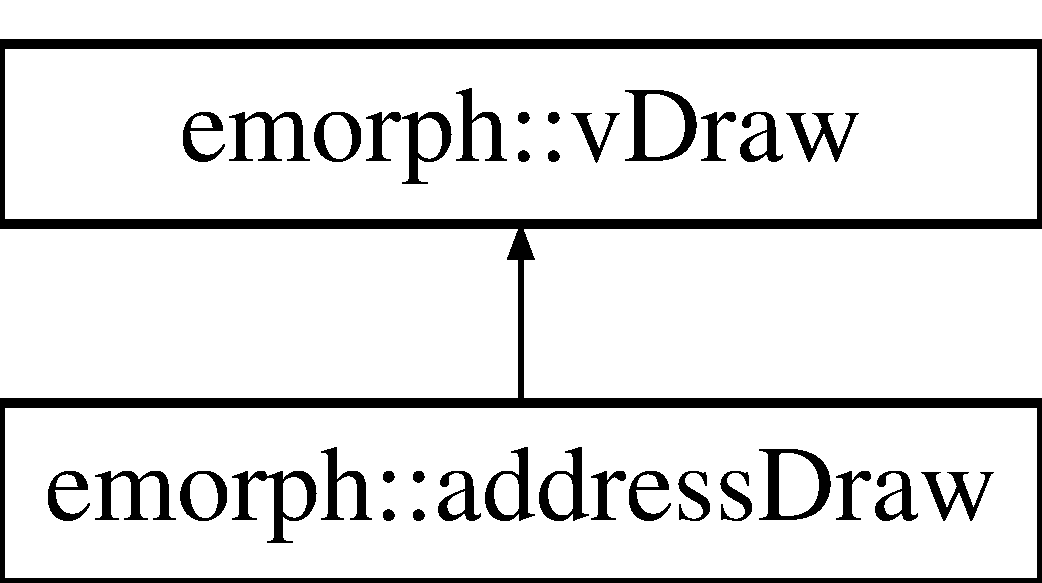
\includegraphics[height=2.000000cm]{classemorph_1_1addressDraw}
\end{center}
\end{figure}
\subsection*{Public Member Functions}
\begin{DoxyCompactItemize}
\item 
\hypertarget{classemorph_1_1addressDraw_a31228f7f61455afb4b7b1536e601c854}{virtual void \hyperlink{classemorph_1_1addressDraw_a31228f7f61455afb4b7b1536e601c854}{draw} (cv\-::\-Mat \&image, const \hyperlink{classemorph_1_1vQueue}{emorph\-::v\-Queue} \&e\-Set)}\label{classemorph_1_1addressDraw_a31228f7f61455afb4b7b1536e601c854}

\begin{DoxyCompactList}\small\item\em see \hyperlink{classemorph_1_1vDraw}{v\-Draw} \end{DoxyCompactList}\item 
\hypertarget{classemorph_1_1addressDraw_a82a6050de6d2950cb6598b0f64cada24}{virtual std\-::string \hyperlink{classemorph_1_1addressDraw_a82a6050de6d2950cb6598b0f64cada24}{get\-Tag} ()}\label{classemorph_1_1addressDraw_a82a6050de6d2950cb6598b0f64cada24}

\begin{DoxyCompactList}\small\item\em see \hyperlink{classemorph_1_1vDraw}{v\-Draw} \end{DoxyCompactList}\end{DoxyCompactItemize}
\subsection*{Additional Inherited Members}


\subsection{Detailed Description}
The \hyperlink{classemorph_1_1addressDraw}{address\-Draw} class is the standard instance of a v\-Drawer that draws simple address events. The \hyperlink{classemorph_1_1addressDraw}{address\-Draw} will completely overwrite any images previously drawn beforehand and thus should always be first in the argument list. 

The documentation for this class was generated from the following files\-:\begin{DoxyCompactItemize}
\item 
/home/aglover/workspace/projects/event\-Driven/src/visualization/v\-Framer/include/i\-Cub/v\-Draw.\-h\item 
/home/aglover/workspace/projects/event\-Driven/src/visualization/v\-Framer/src/v\-Draw.\-cpp\end{DoxyCompactItemize}

\hypertarget{classemorph_1_1AddressEvent}{\section{emorph\-:\-:Address\-Event Class Reference}
\label{classemorph_1_1AddressEvent}\index{emorph\-::\-Address\-Event@{emorph\-::\-Address\-Event}}
}
Inheritance diagram for emorph\-:\-:Address\-Event\-:\begin{figure}[H]
\begin{center}
\leavevmode
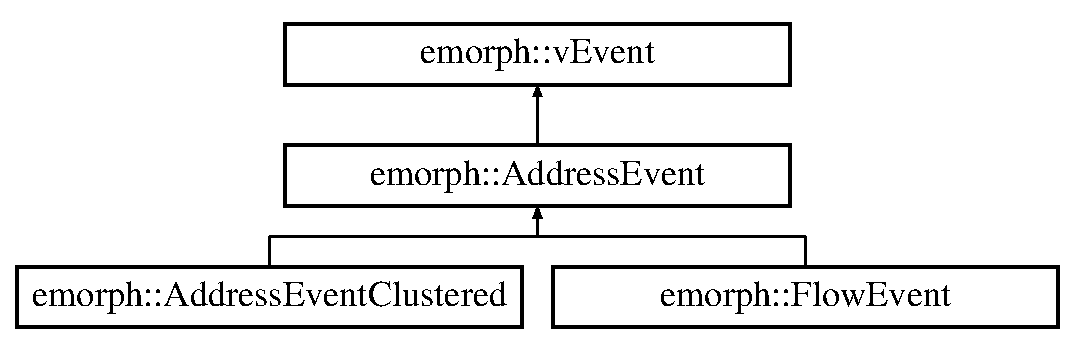
\includegraphics[height=3.000000cm]{classemorph_1_1AddressEvent}
\end{center}
\end{figure}
\subsection*{Public Member Functions}
\begin{DoxyCompactItemize}
\item 
\hypertarget{classemorph_1_1AddressEvent_a9c414ce7baa55a47b12cfe3ef1868526}{virtual std\-::string {\bfseries get\-Type} () const }\label{classemorph_1_1AddressEvent_a9c414ce7baa55a47b12cfe3ef1868526}

\item 
\hypertarget{classemorph_1_1AddressEvent_a231fb70889293b3d4b875bbd56af34a0}{int {\bfseries get\-Channel} () const }\label{classemorph_1_1AddressEvent_a231fb70889293b3d4b875bbd56af34a0}

\item 
\hypertarget{classemorph_1_1AddressEvent_a0e84ab5bf9533555c3950c0121d5ede2}{int {\bfseries get\-Polarity} () const }\label{classemorph_1_1AddressEvent_a0e84ab5bf9533555c3950c0121d5ede2}

\item 
\hypertarget{classemorph_1_1AddressEvent_a9cb757a57b7636d3df4e97be81fb9ce1}{unsigned char {\bfseries get\-X} () const }\label{classemorph_1_1AddressEvent_a9cb757a57b7636d3df4e97be81fb9ce1}

\item 
\hypertarget{classemorph_1_1AddressEvent_a45a4341c3664f57f400816a37d3b9d61}{unsigned char {\bfseries get\-Y} () const }\label{classemorph_1_1AddressEvent_a45a4341c3664f57f400816a37d3b9d61}

\item 
\hypertarget{classemorph_1_1AddressEvent_a6f824e27c0ad466672a50dc32c757f22}{void {\bfseries set\-Channel} (const unsigned char channel)}\label{classemorph_1_1AddressEvent_a6f824e27c0ad466672a50dc32c757f22}

\item 
\hypertarget{classemorph_1_1AddressEvent_ada20d447ba331f85c1960b82c5e0b914}{void {\bfseries set\-Polarity} (const unsigned char polarity)}\label{classemorph_1_1AddressEvent_ada20d447ba331f85c1960b82c5e0b914}

\item 
\hypertarget{classemorph_1_1AddressEvent_a95b9eb0cb8fa36f8eda38843d64d6208}{void {\bfseries set\-X} (const unsigned char x)}\label{classemorph_1_1AddressEvent_a95b9eb0cb8fa36f8eda38843d64d6208}

\item 
\hypertarget{classemorph_1_1AddressEvent_a7044b37fd43e276051478d33399f6c24}{void {\bfseries set\-Y} (const unsigned char y)}\label{classemorph_1_1AddressEvent_a7044b37fd43e276051478d33399f6c24}

\item 
\hypertarget{classemorph_1_1AddressEvent_a2d66de1ff1337f85dbeea02a8dd3593a}{{\bfseries Address\-Event} (const \hyperlink{classemorph_1_1vEvent}{v\-Event} \&event)}\label{classemorph_1_1AddressEvent_a2d66de1ff1337f85dbeea02a8dd3593a}

\item 
\hypertarget{classemorph_1_1AddressEvent_a60eaa995ddad3ee214374c9d85fe504b}{\hyperlink{classemorph_1_1vEvent}{v\-Event} \& {\bfseries operator=} (const \hyperlink{classemorph_1_1vEvent}{v\-Event} \&event)}\label{classemorph_1_1AddressEvent_a60eaa995ddad3ee214374c9d85fe504b}

\item 
\hypertarget{classemorph_1_1AddressEvent_a667127ea5d12dca95037dc1763998b95}{virtual \hyperlink{classemorph_1_1vEvent}{v\-Event} $\ast$ {\bfseries clone} ()}\label{classemorph_1_1AddressEvent_a667127ea5d12dca95037dc1763998b95}

\item 
\hypertarget{classemorph_1_1AddressEvent_a6fc6fbf9415b4551eee250a843f64312}{bool {\bfseries operator==} (const \hyperlink{classemorph_1_1AddressEvent}{Address\-Event} \&event)}\label{classemorph_1_1AddressEvent_a6fc6fbf9415b4551eee250a843f64312}

\item 
\hypertarget{classemorph_1_1AddressEvent_a2bd2c1efef5bdb293577886d1c84da16}{bool {\bfseries operator==} (const \hyperlink{classemorph_1_1vEvent}{v\-Event} \&event)}\label{classemorph_1_1AddressEvent_a2bd2c1efef5bdb293577886d1c84da16}

\item 
\hypertarget{classemorph_1_1AddressEvent_aa8e6e3a1eade9d3607c24dfcce5612b1}{virtual void {\bfseries encode} (yarp\-::os\-::\-Bottle \&b) const }\label{classemorph_1_1AddressEvent_aa8e6e3a1eade9d3607c24dfcce5612b1}

\item 
\hypertarget{classemorph_1_1AddressEvent_a275846fcc224290de0f3bbb567ced038}{yarp\-::os\-::\-Property {\bfseries get\-Content} () const }\label{classemorph_1_1AddressEvent_a275846fcc224290de0f3bbb567ced038}

\item 
\hypertarget{classemorph_1_1AddressEvent_aa725d514b1f3f7ae5609ec2f5b240520}{virtual bool {\bfseries decode} (const yarp\-::os\-::\-Bottle \&packet, int \&pos)}\label{classemorph_1_1AddressEvent_aa725d514b1f3f7ae5609ec2f5b240520}

\item 
\hypertarget{classemorph_1_1AddressEvent_ac7957d7d29a2290d9b572c088a9995dd}{virtual int {\bfseries n\-Bytes\-Coded} () const }\label{classemorph_1_1AddressEvent_ac7957d7d29a2290d9b572c088a9995dd}

\end{DoxyCompactItemize}
\subsection*{Protected Attributes}
\begin{DoxyCompactItemize}
\item 
\hypertarget{classemorph_1_1AddressEvent_a425374ba06cfee6d2b44a6f94ff9b2e3}{char {\bfseries channel}}\label{classemorph_1_1AddressEvent_a425374ba06cfee6d2b44a6f94ff9b2e3}

\item 
\hypertarget{classemorph_1_1AddressEvent_ac362a62aa417cee5e40caad8465299d3}{unsigned char {\bfseries polarity}}\label{classemorph_1_1AddressEvent_ac362a62aa417cee5e40caad8465299d3}

\item 
\hypertarget{classemorph_1_1AddressEvent_a4bdcf2b526b12d92a08586dae5efdd80}{unsigned char {\bfseries x}}\label{classemorph_1_1AddressEvent_a4bdcf2b526b12d92a08586dae5efdd80}

\item 
\hypertarget{classemorph_1_1AddressEvent_a1ad1697a4c2460385bd6a266304feec1}{unsigned char {\bfseries y}}\label{classemorph_1_1AddressEvent_a1ad1697a4c2460385bd6a266304feec1}

\end{DoxyCompactItemize}
\subsection*{Additional Inherited Members}


The documentation for this class was generated from the following files\-:\begin{DoxyCompactItemize}
\item 
/home/aglover/workspace/projects/event\-Driven/emorph\-\_\-lib/include/i\-Cub/emorph/v\-Codec.\-h\item 
/home/aglover/workspace/projects/event\-Driven/emorph\-\_\-lib/src/v\-Codec.\-cpp\end{DoxyCompactItemize}

\hypertarget{classemorph_1_1AddressEventClustered}{\section{emorph\-:\-:Address\-Event\-Clustered Class Reference}
\label{classemorph_1_1AddressEventClustered}\index{emorph\-::\-Address\-Event\-Clustered@{emorph\-::\-Address\-Event\-Clustered}}
}
Inheritance diagram for emorph\-:\-:Address\-Event\-Clustered\-:\begin{figure}[H]
\begin{center}
\leavevmode
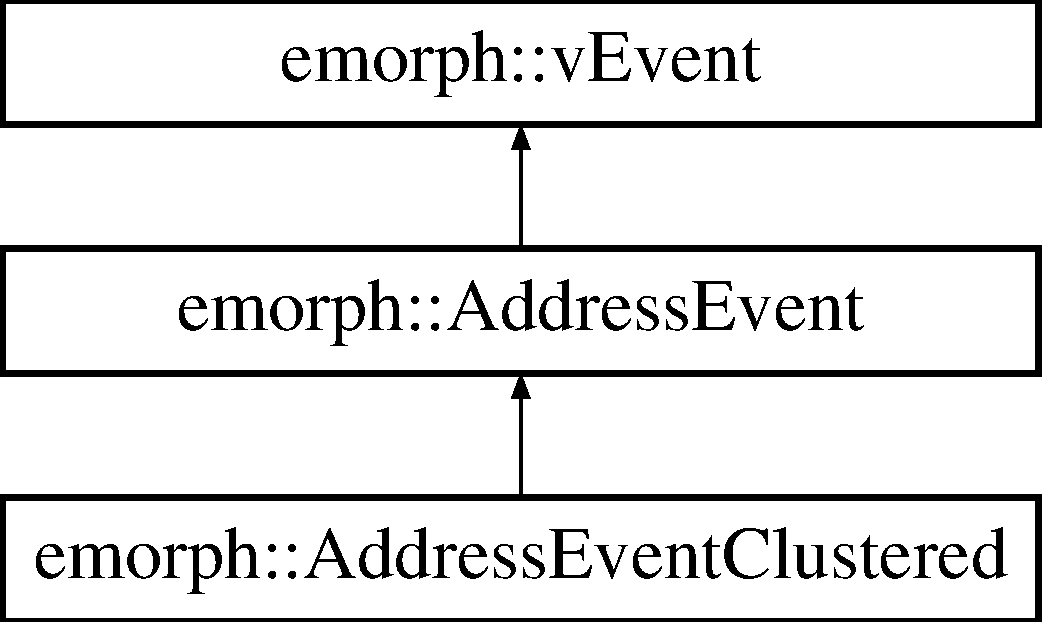
\includegraphics[height=3.000000cm]{classemorph_1_1AddressEventClustered}
\end{center}
\end{figure}
\subsection*{Public Member Functions}
\begin{DoxyCompactItemize}
\item 
\hypertarget{classemorph_1_1AddressEventClustered_ab15c5a4a15575e5e501561f30024e6a9}{virtual std\-::string {\bfseries get\-Type} () const }\label{classemorph_1_1AddressEventClustered_ab15c5a4a15575e5e501561f30024e6a9}

\item 
\hypertarget{classemorph_1_1AddressEventClustered_a5c41b9fb439e9426df7c0905524613bb}{int {\bfseries get\-I\-D} () const }\label{classemorph_1_1AddressEventClustered_a5c41b9fb439e9426df7c0905524613bb}

\item 
\hypertarget{classemorph_1_1AddressEventClustered_aa0e78c11077e59e72c668240af137736}{void {\bfseries set\-I\-D} (const int cl\-I\-D)}\label{classemorph_1_1AddressEventClustered_aa0e78c11077e59e72c668240af137736}

\item 
\hypertarget{classemorph_1_1AddressEventClustered_a5b7af943ce1438eb599534ef34fa7cd5}{{\bfseries Address\-Event\-Clustered} (const \hyperlink{classemorph_1_1vEvent}{v\-Event} \&event)}\label{classemorph_1_1AddressEventClustered_a5b7af943ce1438eb599534ef34fa7cd5}

\item 
\hypertarget{classemorph_1_1AddressEventClustered_af62943d8c4759b5525a11d03fd1048ab}{\hyperlink{classemorph_1_1vEvent}{v\-Event} \& {\bfseries operator=} (const \hyperlink{classemorph_1_1vEvent}{v\-Event} \&event)}\label{classemorph_1_1AddressEventClustered_af62943d8c4759b5525a11d03fd1048ab}

\item 
\hypertarget{classemorph_1_1AddressEventClustered_a07cbe4c77027546a0b62d827c9993827}{virtual \hyperlink{classemorph_1_1vEvent}{v\-Event} $\ast$ {\bfseries clone} ()}\label{classemorph_1_1AddressEventClustered_a07cbe4c77027546a0b62d827c9993827}

\item 
\hypertarget{classemorph_1_1AddressEventClustered_ab79d067ee13c48910150364998572632}{bool {\bfseries operator==} (const \hyperlink{classemorph_1_1AddressEventClustered}{Address\-Event\-Clustered} \&event)}\label{classemorph_1_1AddressEventClustered_ab79d067ee13c48910150364998572632}

\item 
\hypertarget{classemorph_1_1AddressEventClustered_a14885a84ec35ac6ac3b7b012fa89b9f8}{bool {\bfseries operator==} (const \hyperlink{classemorph_1_1vEvent}{v\-Event} \&event)}\label{classemorph_1_1AddressEventClustered_a14885a84ec35ac6ac3b7b012fa89b9f8}

\item 
\hypertarget{classemorph_1_1AddressEventClustered_ae818cd56d2c40e94f47df51890f24fb7}{virtual void {\bfseries encode} (yarp\-::os\-::\-Bottle \&b) const }\label{classemorph_1_1AddressEventClustered_ae818cd56d2c40e94f47df51890f24fb7}

\item 
\hypertarget{classemorph_1_1AddressEventClustered_ab1727071825261bfd230c224ce083433}{yarp\-::os\-::\-Property {\bfseries get\-Content} () const }\label{classemorph_1_1AddressEventClustered_ab1727071825261bfd230c224ce083433}

\item 
\hypertarget{classemorph_1_1AddressEventClustered_a84755ba69f9e2c4b5dcfc847fab04d88}{virtual bool {\bfseries decode} (const yarp\-::os\-::\-Bottle \&packet, int \&pos)}\label{classemorph_1_1AddressEventClustered_a84755ba69f9e2c4b5dcfc847fab04d88}

\item 
\hypertarget{classemorph_1_1AddressEventClustered_a02b5c1553f0b70fbf3207bc3924f626b}{virtual int {\bfseries n\-Bytes\-Coded} () const }\label{classemorph_1_1AddressEventClustered_a02b5c1553f0b70fbf3207bc3924f626b}

\end{DoxyCompactItemize}
\subsection*{Protected Attributes}
\begin{DoxyCompactItemize}
\item 
\hypertarget{classemorph_1_1AddressEventClustered_a9a4298a0e0e0390650289179cb52c24b}{int {\bfseries cl\-I\-D}}\label{classemorph_1_1AddressEventClustered_a9a4298a0e0e0390650289179cb52c24b}

\end{DoxyCompactItemize}
\subsection*{Additional Inherited Members}


The documentation for this class was generated from the following files\-:\begin{DoxyCompactItemize}
\item 
/home/aglover/workspace/projects/event\-Driven/emorph\-\_\-lib/include/i\-Cub/emorph/v\-Codec.\-h\item 
/home/aglover/workspace/projects/event\-Driven/emorph\-\_\-lib/src/v\-Codec.\-cpp\end{DoxyCompactItemize}

\hypertarget{structaer}{\section{aer Struct Reference}
\label{structaer}\index{aer@{aer}}
}
\subsection*{Public Attributes}
\begin{DoxyCompactItemize}
\item 
\hypertarget{structaer_a74e35f1258f6c79df0b88f2544c36b7d}{u32 {\bfseries timestamp}}\label{structaer_a74e35f1258f6c79df0b88f2544c36b7d}

\item 
\hypertarget{structaer_a427837e13cd5ba64e6e70552b6e3e78f}{u32 {\bfseries address}}\label{structaer_a427837e13cd5ba64e6e70552b6e3e78f}

\end{DoxyCompactItemize}


The documentation for this struct was generated from the following file\-:\begin{DoxyCompactItemize}
\item 
/home/aglover/workspace/projects/event\-Driven/src/grabbers/aex\-Grabber/include/i\-Cub/device2yarp.\-h\end{DoxyCompactItemize}

\hypertarget{classaerDevManager}{\section{aer\-Dev\-Manager Class Reference}
\label{classaerDevManager}\index{aer\-Dev\-Manager@{aer\-Dev\-Manager}}
}
Inheritance diagram for aer\-Dev\-Manager\-:\begin{figure}[H]
\begin{center}
\leavevmode
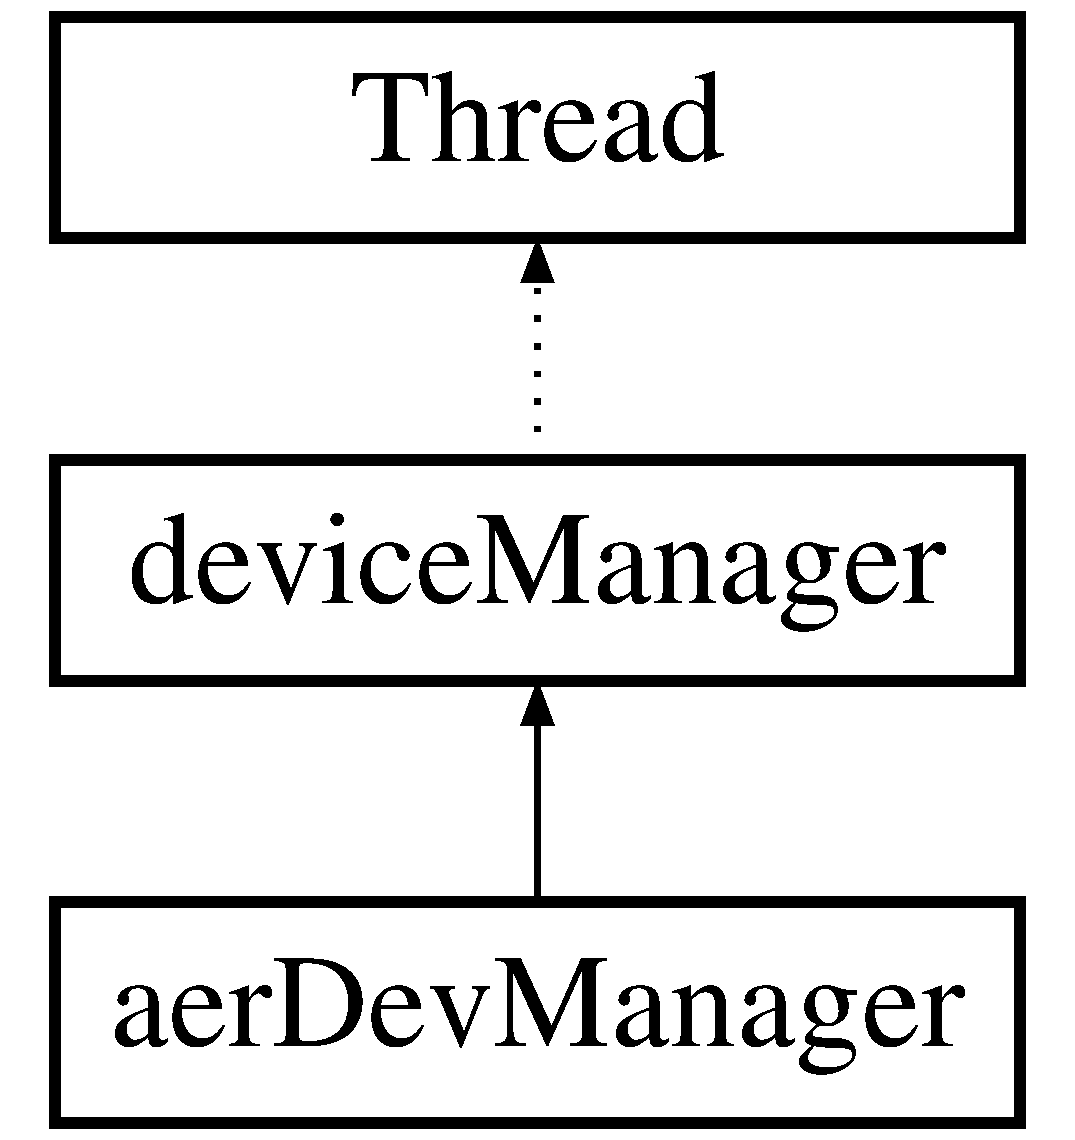
\includegraphics[height=3.000000cm]{classaerDevManager}
\end{center}
\end{figure}
\subsection*{Public Member Functions}
\begin{DoxyCompactItemize}
\item 
\hypertarget{classaerDevManager_a3114113a72907c80d397959c1306e8d6}{{\bfseries aer\-Dev\-Manager} (std\-::string dev)}\label{classaerDevManager_a3114113a72907c80d397959c1306e8d6}

\item 
\hypertarget{classaerDevManager_ab6382b0978b9c7db2efde105c27cac5a}{virtual bool {\bfseries open\-Device} ()}\label{classaerDevManager_ab6382b0978b9c7db2efde105c27cac5a}

\item 
\hypertarget{classaerDevManager_ad5b901f414b292b2a18289abdd0486b1}{virtual void {\bfseries close\-Device} ()}\label{classaerDevManager_ad5b901f414b292b2a18289abdd0486b1}

\item 
\hypertarget{classaerDevManager_a3c73a8e16c315157801c9bf75e70fc53}{void {\bfseries write\-\_\-generic\-\_\-sp2neu\-\_\-reg} (int dev\-Desc, unsigned int offset, unsigned int data)}\label{classaerDevManager_a3c73a8e16c315157801c9bf75e70fc53}

\item 
\hypertarget{classaerDevManager_a22005a9f33a1c2ae5e8594b9b42293b9}{unsigned int {\bfseries read\-\_\-generic\-\_\-sp2neu\-\_\-reg} (int dev\-Desc, unsigned int offset)}\label{classaerDevManager_a22005a9f33a1c2ae5e8594b9b42293b9}

\item 
\hypertarget{classaerDevManager_ae31bd6618aeb35b6559d1dc0d405b8c3}{void {\bfseries usage} (void)}\label{classaerDevManager_ae31bd6618aeb35b6559d1dc0d405b8c3}

\item 
\hypertarget{classaerDevManager_a995c294f2358ceba18af3a92d4667bd0}{bool {\bfseries read\-Fifo\-Full} ()}\label{classaerDevManager_a995c294f2358ceba18af3a92d4667bd0}

\item 
\hypertarget{classaerDevManager_a814e9fc1f2f2b9be6e35af2e9e4556c2}{bool {\bfseries read\-Fifo\-Empty} ()}\label{classaerDevManager_a814e9fc1f2f2b9be6e35af2e9e4556c2}

\item 
\hypertarget{classaerDevManager_a2bcc580c4902eae1083e84576fe3fe2c}{bool {\bfseries write\-Fifo\-A\-Full} ()}\label{classaerDevManager_a2bcc580c4902eae1083e84576fe3fe2c}

\item 
\hypertarget{classaerDevManager_a43bf479627c366e50909fb3b1d7de785}{bool {\bfseries write\-Fifo\-Full} ()}\label{classaerDevManager_a43bf479627c366e50909fb3b1d7de785}

\item 
\hypertarget{classaerDevManager_a9dcf809a01b3a3ab93f9a0a73113a8a0}{bool {\bfseries write\-Fifo\-Empty} ()}\label{classaerDevManager_a9dcf809a01b3a3ab93f9a0a73113a8a0}

\item 
\hypertarget{classaerDevManager_a3e3361083ce17907c2c190fac753c2ef}{int {\bfseries time\-Wrap\-Count} ()}\label{classaerDevManager_a3e3361083ce17907c2c190fac753c2ef}

\end{DoxyCompactItemize}
\subsection*{Additional Inherited Members}


The documentation for this class was generated from the following files\-:\begin{DoxyCompactItemize}
\item 
/home/aglover/workspace/projects/event\-Driven/src/grabbers/zynq\-Grabber/include/i\-Cub/device\-Manager.\-h\item 
/home/aglover/workspace/projects/event\-Driven/src/grabbers/zynq\-Grabber/src/device\-Manager.\-cpp\end{DoxyCompactItemize}

\hypertarget{classaerfx2__0DevManager}{\section{aerfx2\-\_\-0\-Dev\-Manager Class Reference}
\label{classaerfx2__0DevManager}\index{aerfx2\-\_\-0\-Dev\-Manager@{aerfx2\-\_\-0\-Dev\-Manager}}
}
Inheritance diagram for aerfx2\-\_\-0\-Dev\-Manager\-:\begin{figure}[H]
\begin{center}
\leavevmode
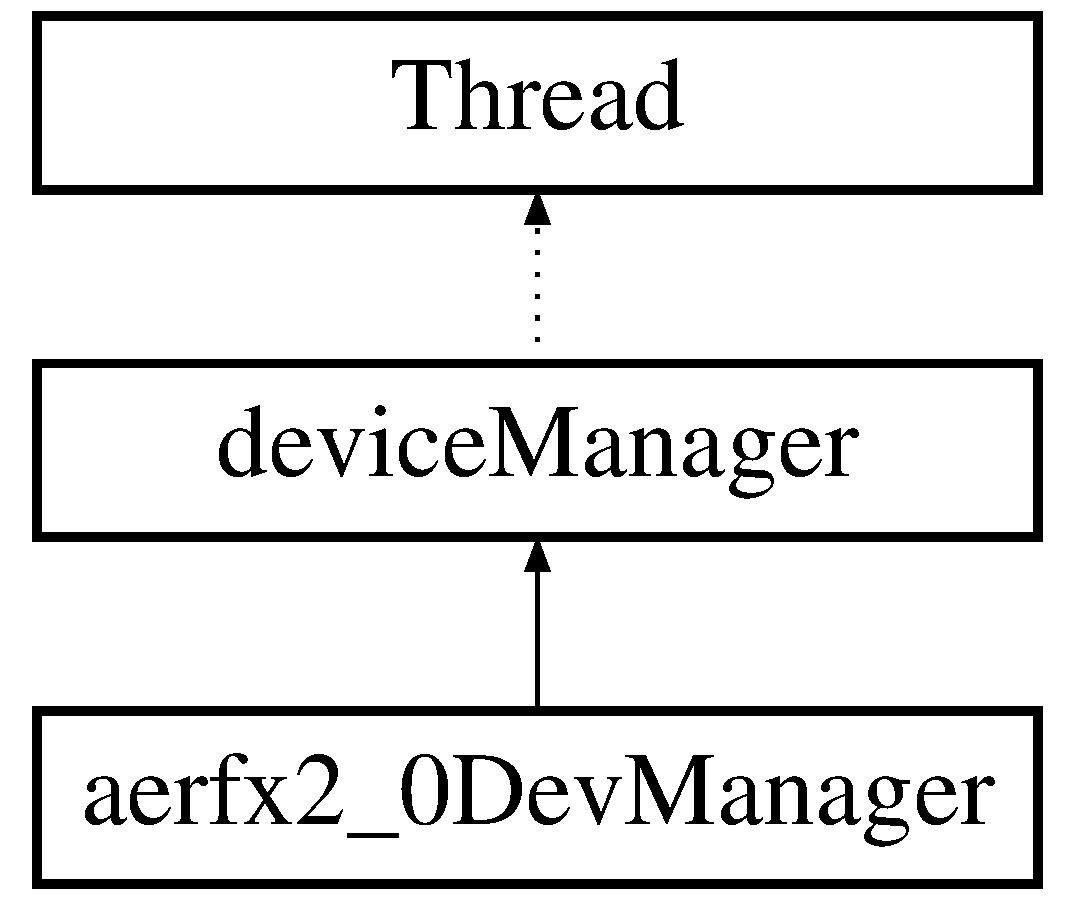
\includegraphics[height=3.000000cm]{classaerfx2__0DevManager}
\end{center}
\end{figure}
\subsection*{Public Member Functions}
\begin{DoxyCompactItemize}
\item 
\hypertarget{classaerfx2__0DevManager_a93dd53b43522a48a10d87bd1e86fed6c}{virtual bool {\bfseries open\-Device} ()}\label{classaerfx2__0DevManager_a93dd53b43522a48a10d87bd1e86fed6c}

\end{DoxyCompactItemize}
\subsection*{Additional Inherited Members}


The documentation for this class was generated from the following files\-:\begin{DoxyCompactItemize}
\item 
/home/aglover/workspace/projects/event\-Driven/src/grabbers/zynq\-Grabber/include/i\-Cub/device\-Manager.\-h\item 
/home/aglover/workspace/projects/event\-Driven/src/grabbers/zynq\-Grabber/src/device\-Manager.\-cpp\end{DoxyCompactItemize}

\hypertarget{classaexGrabberModule}{\section{aex\-Grabber\-Module Class Reference}
\label{classaexGrabberModule}\index{aex\-Grabber\-Module@{aex\-Grabber\-Module}}
}
Inheritance diagram for aex\-Grabber\-Module\-:\begin{figure}[H]
\begin{center}
\leavevmode
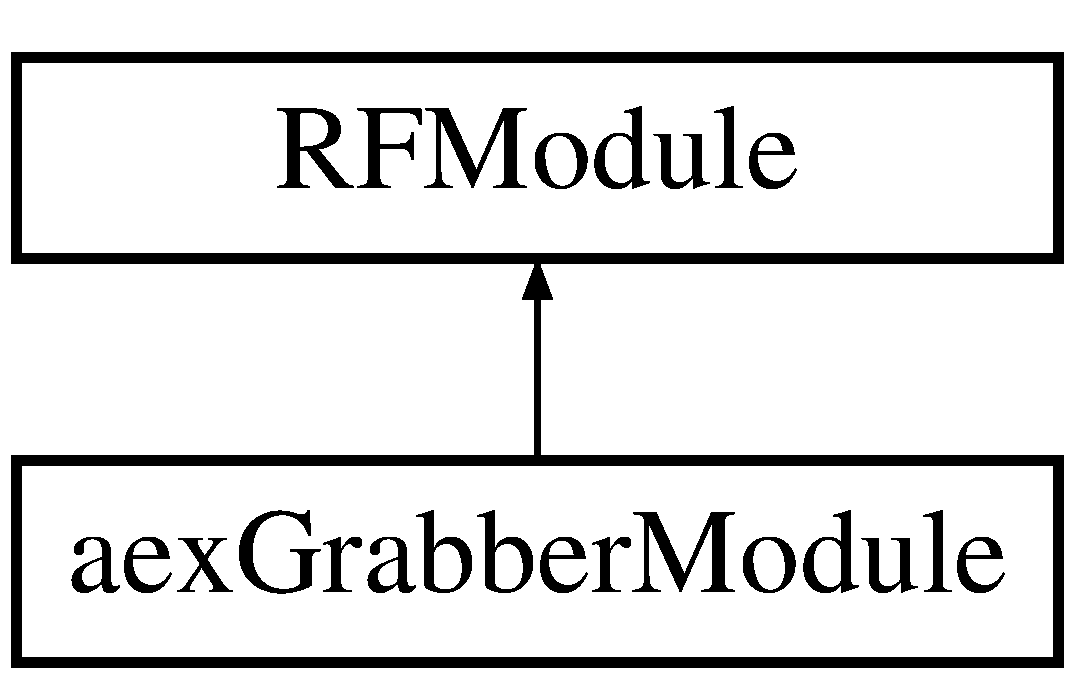
\includegraphics[height=2.000000cm]{classaexGrabberModule}
\end{center}
\end{figure}
\subsection*{Public Member Functions}
\begin{DoxyCompactItemize}
\item 
\hypertarget{classaexGrabberModule_a7654bd490ccdd31ffc5de4e5d85789f3}{bool {\bfseries configure} (yarp\-::os\-::\-Resource\-Finder \&rf)}\label{classaexGrabberModule_a7654bd490ccdd31ffc5de4e5d85789f3}

\item 
\hypertarget{classaexGrabberModule_a349f07e43758979d9f7e520dd25ba868}{bool {\bfseries interrupt\-Module} ()}\label{classaexGrabberModule_a349f07e43758979d9f7e520dd25ba868}

\item 
\hypertarget{classaexGrabberModule_ac032595742ec7bfdd3d6788436572aca}{bool {\bfseries close} ()}\label{classaexGrabberModule_ac032595742ec7bfdd3d6788436572aca}

\item 
\hypertarget{classaexGrabberModule_a18cadf0f324c5dbb7a8d9acfb767ffc0}{bool {\bfseries respond} (const yarp\-::os\-::\-Bottle \&command, yarp\-::os\-::\-Bottle \&reply)}\label{classaexGrabberModule_a18cadf0f324c5dbb7a8d9acfb767ffc0}

\item 
\hypertarget{classaexGrabberModule_a06d7548efce14fbb37945f5640ca029a}{double {\bfseries get\-Period} ()}\label{classaexGrabberModule_a06d7548efce14fbb37945f5640ca029a}

\item 
\hypertarget{classaexGrabberModule_ae08d72931d6f5283092228dab867d92e}{bool {\bfseries update\-Module} ()}\label{classaexGrabberModule_ae08d72931d6f5283092228dab867d92e}

\end{DoxyCompactItemize}


The documentation for this class was generated from the following files\-:\begin{DoxyCompactItemize}
\item 
/home/aglover/workspace/projects/event\-Driven/src/grabbers/aex\-Grabber/include/i\-Cub/aex\-Grabber\-Module.\-h\item 
/home/aglover/workspace/projects/event\-Driven/src/grabbers/aex\-Grabber/src/\hyperlink{aexGrabberModule_8cpp}{aex\-Grabber\-Module.\-cpp}\end{DoxyCompactItemize}

\hypertarget{structatom}{\section{atom Struct Reference}
\label{structatom}\index{atom@{atom}}
}
\subsection*{Public Attributes}
\begin{DoxyCompactItemize}
\item 
\hypertarget{structatom_a54c9c4d5af5fc3f2ca8f14f05917c197}{u32 {\bfseries data}}\label{structatom_a54c9c4d5af5fc3f2ca8f14f05917c197}

\end{DoxyCompactItemize}


The documentation for this struct was generated from the following file\-:\begin{DoxyCompactItemize}
\item 
/home/aglover/workspace/projects/event\-Driven/src/grabbers/aex\-Grabber/include/i\-Cub/device2yarp.\-h\end{DoxyCompactItemize}

\hypertarget{classemorph_1_1blobDraw}{\section{emorph\-:\-:blob\-Draw Class Reference}
\label{classemorph_1_1blobDraw}\index{emorph\-::blob\-Draw@{emorph\-::blob\-Draw}}
}
Inheritance diagram for emorph\-:\-:blob\-Draw\-:\begin{figure}[H]
\begin{center}
\leavevmode
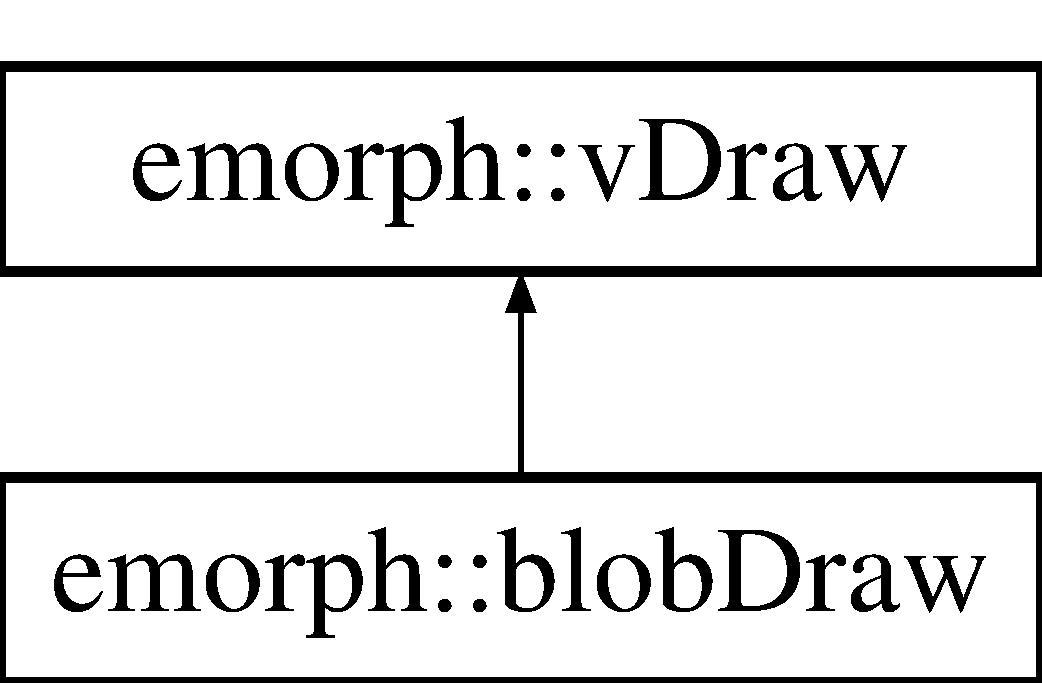
\includegraphics[height=2.000000cm]{classemorph_1_1blobDraw}
\end{center}
\end{figure}
\subsection*{Public Member Functions}
\begin{DoxyCompactItemize}
\item 
\hypertarget{classemorph_1_1blobDraw_af2be44e448d04221db47e9b21b03aeec}{virtual void \hyperlink{classemorph_1_1blobDraw_af2be44e448d04221db47e9b21b03aeec}{draw} (cv\-::\-Mat \&image, const \hyperlink{classemorph_1_1vQueue}{emorph\-::v\-Queue} \&e\-Set)}\label{classemorph_1_1blobDraw_af2be44e448d04221db47e9b21b03aeec}

\begin{DoxyCompactList}\small\item\em see \hyperlink{classemorph_1_1vDraw}{v\-Draw} \end{DoxyCompactList}\item 
\hypertarget{classemorph_1_1blobDraw_ad0970eb3689b4fb08aec786184ec2f92}{virtual std\-::string \hyperlink{classemorph_1_1blobDraw_ad0970eb3689b4fb08aec786184ec2f92}{get\-Tag} ()}\label{classemorph_1_1blobDraw_ad0970eb3689b4fb08aec786184ec2f92}

\begin{DoxyCompactList}\small\item\em see \hyperlink{classemorph_1_1vDraw}{v\-Draw} \end{DoxyCompactList}\end{DoxyCompactItemize}
\subsection*{Additional Inherited Members}


The documentation for this class was generated from the following files\-:\begin{DoxyCompactItemize}
\item 
/home/aglover/workspace/projects/event\-Driven/src/visualization/v\-Framer/include/i\-Cub/v\-Draw.\-h\item 
/home/aglover/workspace/projects/event\-Driven/src/visualization/v\-Framer/src/v\-Draw.\-cpp\end{DoxyCompactItemize}

\hypertarget{classBlobTracker}{\section{Blob\-Tracker Class Reference}
\label{classBlobTracker}\index{Blob\-Tracker@{Blob\-Tracker}}
}
\subsection*{Public Member Functions}
\begin{DoxyCompactItemize}
\item 
\hypertarget{classBlobTracker_ac3dbde755642d5e9cf179123823a8eec}{bool {\bfseries initialise\-Position} (double x, double y)}\label{classBlobTracker_ac3dbde755642d5e9cf179123823a8eec}

\item 
\hypertarget{classBlobTracker_a29990e53b163a720f284978b97a6d723}{bool {\bfseries initialise\-Shape} (double sig\-X, double sig\-Y2, double sig\-X\-Y, double alpha\-\_\-pos, double alpha\-\_\-shape, bool fix)}\label{classBlobTracker_a29990e53b163a720f284978b97a6d723}

\item 
\hypertarget{classBlobTracker_a873c6f0932845537163a5b80605ac599}{double {\bfseries dist2event} (int ev\-\_\-x, int ev\-\_\-y)}\label{classBlobTracker_a873c6f0932845537163a5b80605ac599}

\item 
\hypertarget{classBlobTracker_abfe11c1db8b5c9634ec9f5ba86f379d9}{double {\bfseries compute\-\_\-p} (int ev\-\_\-x, int ev\-\_\-y)}\label{classBlobTracker_abfe11c1db8b5c9634ec9f5ba86f379d9}

\item 
\hypertarget{classBlobTracker_ab84953899ecee068e63a8f1a89fe7dd8}{bool {\bfseries add\-Activity} (int x, int y, unsigned long int ts, double Tact, double Tevent)}\label{classBlobTracker_ab84953899ecee068e63a8f1a89fe7dd8}

\item 
\hypertarget{classBlobTracker_af410be534735ad33bafc259d70316a54}{bool {\bfseries decay\-Activity} (int dt, double tau, double Tinact, double Tfree)}\label{classBlobTracker_af410be534735ad33bafc259d70316a54}

\item 
\hypertarget{classBlobTracker_af7a07b561d9516ab480632667672e7ed}{void {\bfseries cluster\-Spiked} ()}\label{classBlobTracker_af7a07b561d9516ab480632667672e7ed}

\item 
\hypertarget{classBlobTracker_ad22b6a8aaf647e71b57fba25f9f419d1}{void {\bfseries is\-No\-Longer\-Free} ()}\label{classBlobTracker_ad22b6a8aaf647e71b57fba25f9f419d1}

\item 
\hypertarget{classBlobTracker_af0cd5a8da431251197c88560c919d89d}{bool {\bfseries is\-\_\-active} ()}\label{classBlobTracker_af0cd5a8da431251197c88560c919d89d}

\item 
\hypertarget{classBlobTracker_a8f18821eb105ce6e95d05e4cc4e3a3aa}{bool {\bfseries is\-\_\-on} ()}\label{classBlobTracker_a8f18821eb105ce6e95d05e4cc4e3a3aa}

\item 
\hypertarget{classBlobTracker_a21f9c5029c220f71e7442a8b068431b7}{bool {\bfseries is\-Free} ()}\label{classBlobTracker_a21f9c5029c220f71e7442a8b068431b7}

\item 
\hypertarget{classBlobTracker_ab42f73b98cb1885cdd162148ace8bf23}{double {\bfseries get\-\_\-sigx2} ()}\label{classBlobTracker_ab42f73b98cb1885cdd162148ace8bf23}

\item 
\hypertarget{classBlobTracker_a6cc4fcfc6ade9a856dc7ba502531adf5}{double {\bfseries get\-\_\-sigy2} ()}\label{classBlobTracker_a6cc4fcfc6ade9a856dc7ba502531adf5}

\item 
\hypertarget{classBlobTracker_aeb6aed3ccd9793682b005127fab2bffd}{double {\bfseries get\-\_\-sigxy} ()}\label{classBlobTracker_aeb6aed3ccd9793682b005127fab2bffd}

\item 
\hypertarget{classBlobTracker_aa20dbabdbbfabb44301d18bc59881488}{int {\bfseries get\-\_\-x} ()}\label{classBlobTracker_aa20dbabdbbfabb44301d18bc59881488}

\item 
\hypertarget{classBlobTracker_a2d78cea632f8f9fa4b325c575b9b49d9}{int {\bfseries get\-\_\-y} ()}\label{classBlobTracker_a2d78cea632f8f9fa4b325c575b9b49d9}

\item 
\hypertarget{classBlobTracker_a339a2cdbf0e3af39241abc7dac115f6c}{double {\bfseries get\-\_\-vx} ()}\label{classBlobTracker_a339a2cdbf0e3af39241abc7dac115f6c}

\item 
\hypertarget{classBlobTracker_a99050a07f515b524837a3977e9c53a9c}{double {\bfseries get\-\_\-vy} ()}\label{classBlobTracker_a99050a07f515b524837a3977e9c53a9c}

\item 
\hypertarget{classBlobTracker_a8b59d7b66e32c3c55486f7ef7446fbde}{double {\bfseries get\-\_\-act} ()}\label{classBlobTracker_a8b59d7b66e32c3c55486f7ef7446fbde}

\end{DoxyCompactItemize}
\subsection*{Protected Types}
\begin{DoxyCompactItemize}
\item 
enum {\bfseries State} \{ {\bfseries Active}, 
{\bfseries Inactive}, 
{\bfseries Free}
 \}
\end{DoxyCompactItemize}
\subsection*{Protected Attributes}
\begin{DoxyCompactItemize}
\item 
\hypertarget{classBlobTracker_ad96c96edcf8e9b2155aba3c39d128249}{State {\bfseries state\-\_\-}}\label{classBlobTracker_ad96c96edcf8e9b2155aba3c39d128249}

\item 
\hypertarget{classBlobTracker_a93b360b9499b9a77c7da2eb0b264d8af}{double {\bfseries cen\-\_\-x\-\_\-}}\label{classBlobTracker_a93b360b9499b9a77c7da2eb0b264d8af}

\item 
\hypertarget{classBlobTracker_ab5eaa89cfedfb25fc0881009cefdbea4}{double {\bfseries cen\-\_\-y\-\_\-}}\label{classBlobTracker_ab5eaa89cfedfb25fc0881009cefdbea4}

\item 
\hypertarget{classBlobTracker_a90039cb4599ff8cf137d0b0a9b89801e}{double {\bfseries sig\-\_\-x2\-\_\-}}\label{classBlobTracker_a90039cb4599ff8cf137d0b0a9b89801e}

\item 
\hypertarget{classBlobTracker_a8fa7fa36db3faed93d94b30bd50449e1}{double {\bfseries sig\-\_\-y2\-\_\-}}\label{classBlobTracker_a8fa7fa36db3faed93d94b30bd50449e1}

\item 
\hypertarget{classBlobTracker_af7c64be12d9aeee877adc6027e57dc31}{double {\bfseries sig\-\_\-xy\-\_\-}}\label{classBlobTracker_af7c64be12d9aeee877adc6027e57dc31}

\item 
\hypertarget{classBlobTracker_a37789b44e5e478a237580a3e168bd496}{double {\bfseries v\-Last\-X}}\label{classBlobTracker_a37789b44e5e478a237580a3e168bd496}

\item 
\hypertarget{classBlobTracker_ae836b9dd8d830ba8f6ccb6ea2f80e313}{double {\bfseries v\-Last\-Y}}\label{classBlobTracker_ae836b9dd8d830ba8f6ccb6ea2f80e313}

\item 
\hypertarget{classBlobTracker_a98a091e1f3a0e16a71ff6602079c9c23}{double {\bfseries vx\-\_\-}}\label{classBlobTracker_a98a091e1f3a0e16a71ff6602079c9c23}

\item 
\hypertarget{classBlobTracker_a5b41c1c66d14c8b794b314ba204a93bd}{double {\bfseries vy\-\_\-}}\label{classBlobTracker_a5b41c1c66d14c8b794b314ba204a93bd}

\item 
\hypertarget{classBlobTracker_ae10a65c546bfa9ed53d341a46080f53f}{double {\bfseries alpha\-\_\-pos\-\_\-}}\label{classBlobTracker_ae10a65c546bfa9ed53d341a46080f53f}

\item 
\hypertarget{classBlobTracker_a5183d2c99bd9dbc6f7170050e5830dea}{double {\bfseries alpha\-\_\-shape\-\_\-}}\label{classBlobTracker_a5183d2c99bd9dbc6f7170050e5830dea}

\item 
\hypertarget{classBlobTracker_a57841b67cf49324e2ff7b9698897e908}{bool {\bfseries fixed\-\_\-shape\-\_\-}}\label{classBlobTracker_a57841b67cf49324e2ff7b9698897e908}

\item 
\hypertarget{classBlobTracker_aaf83587414449f41fa7719f9939c48a8}{double {\bfseries activity\-\_\-}}\label{classBlobTracker_aaf83587414449f41fa7719f9939c48a8}

\item 
\hypertarget{classBlobTracker_a4084fae015313204286ce98259856467}{unsigned long int {\bfseries ts\-\_\-last\-\_\-update\-\_\-}}\label{classBlobTracker_a4084fae015313204286ce98259856467}

\end{DoxyCompactItemize}


The documentation for this class was generated from the following files\-:\begin{DoxyCompactItemize}
\item 
/home/aglover/workspace/projects/event\-Driven/src/processing/v\-Cluster/include/blob\-Tracker.\-h\item 
/home/aglover/workspace/projects/event\-Driven/src/processing/v\-Cluster/src/blob\-Tracker.\-cpp\end{DoxyCompactItemize}

\hypertarget{classemorph_1_1circleDraw}{\section{emorph\-:\-:circle\-Draw Class Reference}
\label{classemorph_1_1circleDraw}\index{emorph\-::circle\-Draw@{emorph\-::circle\-Draw}}
}
Inheritance diagram for emorph\-:\-:circle\-Draw\-:\begin{figure}[H]
\begin{center}
\leavevmode
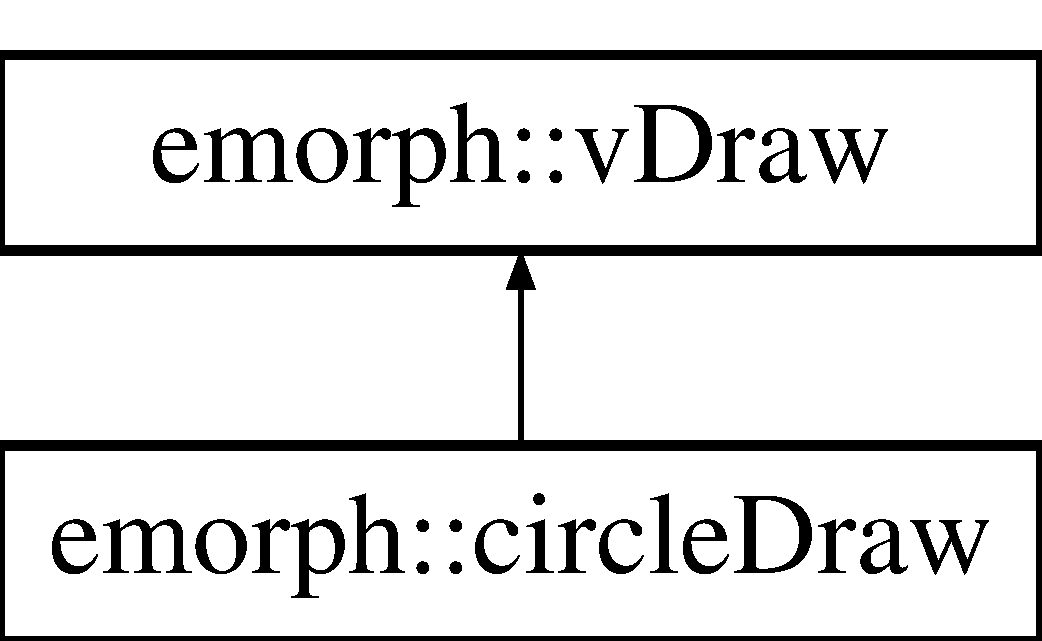
\includegraphics[height=2.000000cm]{classemorph_1_1circleDraw}
\end{center}
\end{figure}
\subsection*{Public Member Functions}
\begin{DoxyCompactItemize}
\item 
\hypertarget{classemorph_1_1circleDraw_a03dde28736c280049798d5f9619a8be5}{virtual void \hyperlink{classemorph_1_1circleDraw_a03dde28736c280049798d5f9619a8be5}{draw} (cv\-::\-Mat \&image, const \hyperlink{classemorph_1_1vQueue}{emorph\-::v\-Queue} \&e\-Set)}\label{classemorph_1_1circleDraw_a03dde28736c280049798d5f9619a8be5}

\begin{DoxyCompactList}\small\item\em see \hyperlink{classemorph_1_1vDraw}{v\-Draw} \end{DoxyCompactList}\item 
\hypertarget{classemorph_1_1circleDraw_ae725bd75bc70f72c14c1d01e0365080b}{virtual std\-::string \hyperlink{classemorph_1_1circleDraw_ae725bd75bc70f72c14c1d01e0365080b}{get\-Tag} ()}\label{classemorph_1_1circleDraw_ae725bd75bc70f72c14c1d01e0365080b}

\begin{DoxyCompactList}\small\item\em see \hyperlink{classemorph_1_1vDraw}{v\-Draw} \end{DoxyCompactList}\end{DoxyCompactItemize}
\subsection*{Additional Inherited Members}


The documentation for this class was generated from the following files\-:\begin{DoxyCompactItemize}
\item 
/home/aglover/workspace/projects/event\-Driven/src/visualization/v\-Framer/include/i\-Cub/v\-Draw.\-h\item 
/home/aglover/workspace/projects/event\-Driven/src/visualization/v\-Framer/src/v\-Draw.\-cpp\end{DoxyCompactItemize}

\hypertarget{classemorph_1_1clusterDraw}{\section{emorph\-:\-:cluster\-Draw Class Reference}
\label{classemorph_1_1clusterDraw}\index{emorph\-::cluster\-Draw@{emorph\-::cluster\-Draw}}
}


The cluster\-Drawer overlays the image with visualisation of event clusters.  




{\ttfamily \#include $<$v\-Draw.\-h$>$}

Inheritance diagram for emorph\-:\-:cluster\-Draw\-:\begin{figure}[H]
\begin{center}
\leavevmode
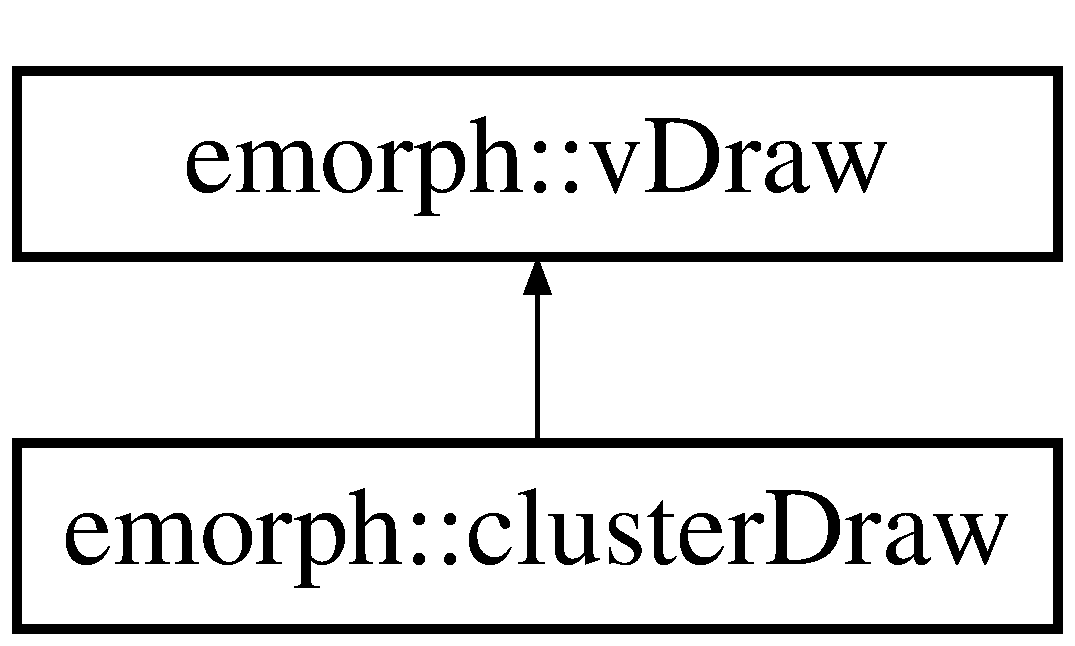
\includegraphics[height=2.000000cm]{classemorph_1_1clusterDraw}
\end{center}
\end{figure}
\subsection*{Public Member Functions}
\begin{DoxyCompactItemize}
\item 
\hypertarget{classemorph_1_1clusterDraw_a79e1d35439561ce08431da19a480e88c}{virtual void \hyperlink{classemorph_1_1clusterDraw_a79e1d35439561ce08431da19a480e88c}{draw} (cv\-::\-Mat \&image, const \hyperlink{classemorph_1_1vQueue}{emorph\-::v\-Queue} \&e\-Set)}\label{classemorph_1_1clusterDraw_a79e1d35439561ce08431da19a480e88c}

\begin{DoxyCompactList}\small\item\em see \hyperlink{classemorph_1_1vDraw}{v\-Draw} \end{DoxyCompactList}\item 
\hypertarget{classemorph_1_1clusterDraw_a2b6aff21bcfc2088f8b580ee8a0e74ba}{virtual std\-::string \hyperlink{classemorph_1_1clusterDraw_a2b6aff21bcfc2088f8b580ee8a0e74ba}{get\-Tag} ()}\label{classemorph_1_1clusterDraw_a2b6aff21bcfc2088f8b580ee8a0e74ba}

\begin{DoxyCompactList}\small\item\em see \hyperlink{classemorph_1_1vDraw}{v\-Draw} \end{DoxyCompactList}\end{DoxyCompactItemize}
\subsection*{Protected Attributes}
\begin{DoxyCompactItemize}
\item 
\hypertarget{classemorph_1_1clusterDraw_aa11ffa556c87a09201503826bce2317c}{std\-::map$<$ int, \\*
\hyperlink{classemorph_1_1ClusterEvent}{emorph\-::\-Cluster\-Event} $\ast$ $>$ {\bfseries persistance}}\label{classemorph_1_1clusterDraw_aa11ffa556c87a09201503826bce2317c}

\item 
\hypertarget{classemorph_1_1clusterDraw_a34d64c050eb0fe5a078c5903bb3c9779}{int {\bfseries stagnant\-Count}}\label{classemorph_1_1clusterDraw_a34d64c050eb0fe5a078c5903bb3c9779}

\end{DoxyCompactItemize}
\subsection*{Additional Inherited Members}


\subsection{Detailed Description}
The cluster\-Drawer overlays the image with visualisation of event clusters. 

The documentation for this class was generated from the following files\-:\begin{DoxyCompactItemize}
\item 
/home/aglover/workspace/projects/event\-Driven/src/visualization/v\-Framer/include/i\-Cub/v\-Draw.\-h\item 
/home/aglover/workspace/projects/event\-Driven/src/visualization/v\-Framer/src/v\-Draw.\-cpp\end{DoxyCompactItemize}

\hypertarget{classemorph_1_1ClusterEvent}{\section{emorph\-:\-:Cluster\-Event Class Reference}
\label{classemorph_1_1ClusterEvent}\index{emorph\-::\-Cluster\-Event@{emorph\-::\-Cluster\-Event}}
}
Inheritance diagram for emorph\-:\-:Cluster\-Event\-:\begin{figure}[H]
\begin{center}
\leavevmode
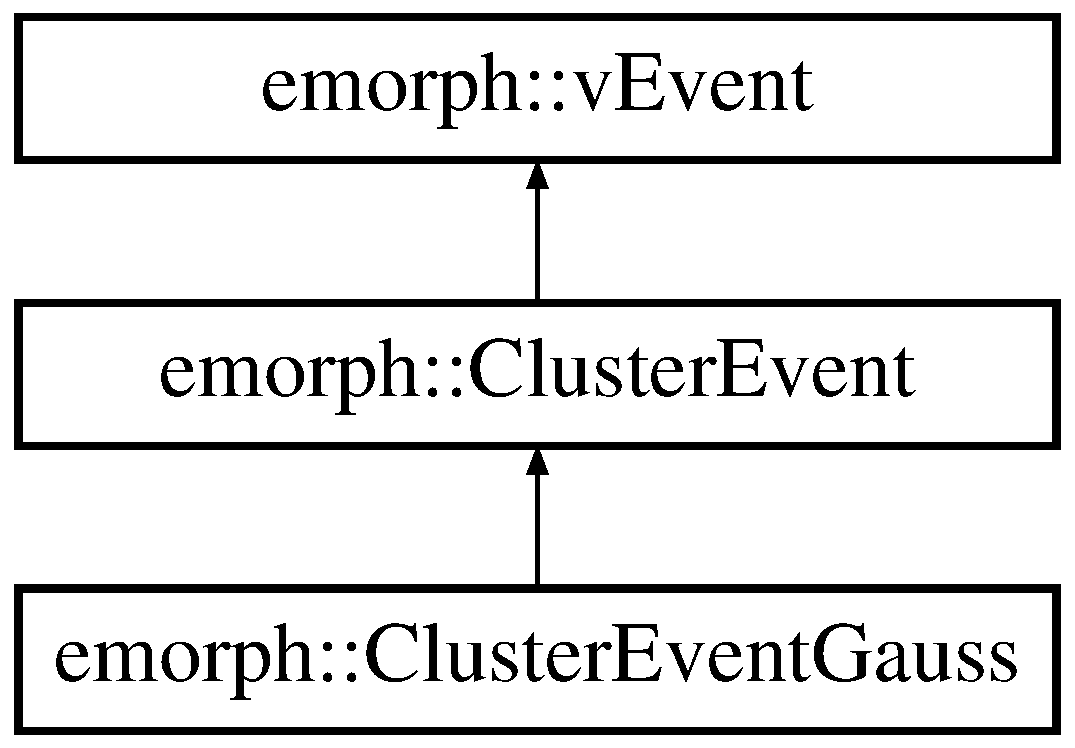
\includegraphics[height=3.000000cm]{classemorph_1_1ClusterEvent}
\end{center}
\end{figure}
\subsection*{Public Member Functions}
\begin{DoxyCompactItemize}
\item 
\hypertarget{classemorph_1_1ClusterEvent_a122c9c8d5c0fd44f011781585436347a}{virtual std\-::string {\bfseries get\-Type} () const }\label{classemorph_1_1ClusterEvent_a122c9c8d5c0fd44f011781585436347a}

\item 
\hypertarget{classemorph_1_1ClusterEvent_af2f6343d948ad071557d5d59f856d4a7}{int {\bfseries get\-Channel} () const }\label{classemorph_1_1ClusterEvent_af2f6343d948ad071557d5d59f856d4a7}

\item 
\hypertarget{classemorph_1_1ClusterEvent_ae8e282dd4aad4b3d6bc38105abd40eb7}{int {\bfseries get\-I\-D} () const }\label{classemorph_1_1ClusterEvent_ae8e282dd4aad4b3d6bc38105abd40eb7}

\item 
\hypertarget{classemorph_1_1ClusterEvent_a89a9ea0163e44f3f50bc15d23d63b3e6}{int {\bfseries get\-X\-Cog} () const }\label{classemorph_1_1ClusterEvent_a89a9ea0163e44f3f50bc15d23d63b3e6}

\item 
\hypertarget{classemorph_1_1ClusterEvent_aec7421372a0150f41b5a6d8bea678a9c}{int {\bfseries get\-Y\-Cog} () const }\label{classemorph_1_1ClusterEvent_aec7421372a0150f41b5a6d8bea678a9c}

\item 
\hypertarget{classemorph_1_1ClusterEvent_aef47e3ab7bfa024b0ea2e66db9c2f48c}{int {\bfseries get\-Polarity} () const }\label{classemorph_1_1ClusterEvent_aef47e3ab7bfa024b0ea2e66db9c2f48c}

\item 
\hypertarget{classemorph_1_1ClusterEvent_a874dd16064761c66c8cd1dcf04c4ee85}{void {\bfseries set\-Channel} (const int channel)}\label{classemorph_1_1ClusterEvent_a874dd16064761c66c8cd1dcf04c4ee85}

\item 
\hypertarget{classemorph_1_1ClusterEvent_a1a29ac36deec29ee952ba19e2067d163}{void {\bfseries set\-I\-D} (const int id)}\label{classemorph_1_1ClusterEvent_a1a29ac36deec29ee952ba19e2067d163}

\item 
\hypertarget{classemorph_1_1ClusterEvent_ab08f800c0e9e411b60b980d437328ac1}{void {\bfseries set\-X\-Cog} (const int x\-Cog)}\label{classemorph_1_1ClusterEvent_ab08f800c0e9e411b60b980d437328ac1}

\item 
\hypertarget{classemorph_1_1ClusterEvent_a4a316c8fa000fa9e84611abd95657614}{void {\bfseries set\-Y\-Cog} (const int y\-Cog)}\label{classemorph_1_1ClusterEvent_a4a316c8fa000fa9e84611abd95657614}

\item 
\hypertarget{classemorph_1_1ClusterEvent_a0fad6fc86fa3216bd25b915803d25ea2}{void {\bfseries set\-Polarity} (const int polarity)}\label{classemorph_1_1ClusterEvent_a0fad6fc86fa3216bd25b915803d25ea2}

\item 
\hypertarget{classemorph_1_1ClusterEvent_afce0907873d034a88b27844d84176ed9}{{\bfseries Cluster\-Event} (const \hyperlink{classemorph_1_1vEvent}{v\-Event} \&event)}\label{classemorph_1_1ClusterEvent_afce0907873d034a88b27844d84176ed9}

\item 
\hypertarget{classemorph_1_1ClusterEvent_ac58b4687be25820727281c5cff6ce02c}{\hyperlink{classemorph_1_1vEvent}{v\-Event} \& {\bfseries operator=} (const \hyperlink{classemorph_1_1vEvent}{v\-Event} \&event)}\label{classemorph_1_1ClusterEvent_ac58b4687be25820727281c5cff6ce02c}

\item 
\hypertarget{classemorph_1_1ClusterEvent_a98c5f0ef6f39f819b440dc8b08e9e625}{virtual \hyperlink{classemorph_1_1vEvent}{v\-Event} $\ast$ {\bfseries clone} ()}\label{classemorph_1_1ClusterEvent_a98c5f0ef6f39f819b440dc8b08e9e625}

\item 
\hypertarget{classemorph_1_1ClusterEvent_a0f73e4a939933c65d4f22b17986bf2f1}{bool {\bfseries operator==} (const \hyperlink{classemorph_1_1ClusterEvent}{Cluster\-Event} \&event)}\label{classemorph_1_1ClusterEvent_a0f73e4a939933c65d4f22b17986bf2f1}

\item 
\hypertarget{classemorph_1_1ClusterEvent_a97b2b246ca4520f05cc79ba276cd5f7d}{bool {\bfseries operator==} (const \hyperlink{classemorph_1_1vEvent}{v\-Event} \&event)}\label{classemorph_1_1ClusterEvent_a97b2b246ca4520f05cc79ba276cd5f7d}

\item 
\hypertarget{classemorph_1_1ClusterEvent_ae31cf2d26bc4e05db7efcd65d078e055}{virtual void {\bfseries encode} (yarp\-::os\-::\-Bottle \&b) const }\label{classemorph_1_1ClusterEvent_ae31cf2d26bc4e05db7efcd65d078e055}

\item 
\hypertarget{classemorph_1_1ClusterEvent_aebb09ecc01dc56514e83340b20be4cdb}{yarp\-::os\-::\-Property {\bfseries get\-Content} () const }\label{classemorph_1_1ClusterEvent_aebb09ecc01dc56514e83340b20be4cdb}

\item 
\hypertarget{classemorph_1_1ClusterEvent_a5b360ff84943c3f8306ad1d6698ef347}{virtual bool {\bfseries decode} (const yarp\-::os\-::\-Bottle \&packet, int \&pos)}\label{classemorph_1_1ClusterEvent_a5b360ff84943c3f8306ad1d6698ef347}

\item 
\hypertarget{classemorph_1_1ClusterEvent_a1e134a3e8f53ffe6521e00a0db66ce0e}{virtual int {\bfseries n\-Bytes\-Coded} () const }\label{classemorph_1_1ClusterEvent_a1e134a3e8f53ffe6521e00a0db66ce0e}

\end{DoxyCompactItemize}
\subsection*{Protected Attributes}
\begin{DoxyCompactItemize}
\item 
\hypertarget{classemorph_1_1ClusterEvent_a885cbc53c2b042e3b9a583ad4f09cbe9}{short int {\bfseries id}}\label{classemorph_1_1ClusterEvent_a885cbc53c2b042e3b9a583ad4f09cbe9}

\item 
\hypertarget{classemorph_1_1ClusterEvent_adae97efa4b50b75a2744cf062e5f0903}{unsigned char {\bfseries channel}}\label{classemorph_1_1ClusterEvent_adae97efa4b50b75a2744cf062e5f0903}

\item 
\hypertarget{classemorph_1_1ClusterEvent_aca2e96418697809fa32ae154b4fa02bb}{unsigned char {\bfseries x\-Cog}}\label{classemorph_1_1ClusterEvent_aca2e96418697809fa32ae154b4fa02bb}

\item 
\hypertarget{classemorph_1_1ClusterEvent_aba3d3d54d58bbb43b73d771a86dc64de}{unsigned char {\bfseries y\-Cog}}\label{classemorph_1_1ClusterEvent_aba3d3d54d58bbb43b73d771a86dc64de}

\item 
\hypertarget{classemorph_1_1ClusterEvent_a77f96e40db5aea2b5346d7c38f6d0aaa}{unsigned char {\bfseries polarity}}\label{classemorph_1_1ClusterEvent_a77f96e40db5aea2b5346d7c38f6d0aaa}

\end{DoxyCompactItemize}
\subsection*{Additional Inherited Members}


The documentation for this class was generated from the following files\-:\begin{DoxyCompactItemize}
\item 
/home/aglover/workspace/projects/event\-Driven/emorph\-\_\-lib/include/i\-Cub/emorph/v\-Codec.\-h\item 
/home/aglover/workspace/projects/event\-Driven/emorph\-\_\-lib/src/v\-Codec.\-cpp\end{DoxyCompactItemize}

\hypertarget{classemorph_1_1ClusterEventGauss}{\section{emorph\-:\-:Cluster\-Event\-Gauss Class Reference}
\label{classemorph_1_1ClusterEventGauss}\index{emorph\-::\-Cluster\-Event\-Gauss@{emorph\-::\-Cluster\-Event\-Gauss}}
}
Inheritance diagram for emorph\-:\-:Cluster\-Event\-Gauss\-:\begin{figure}[H]
\begin{center}
\leavevmode
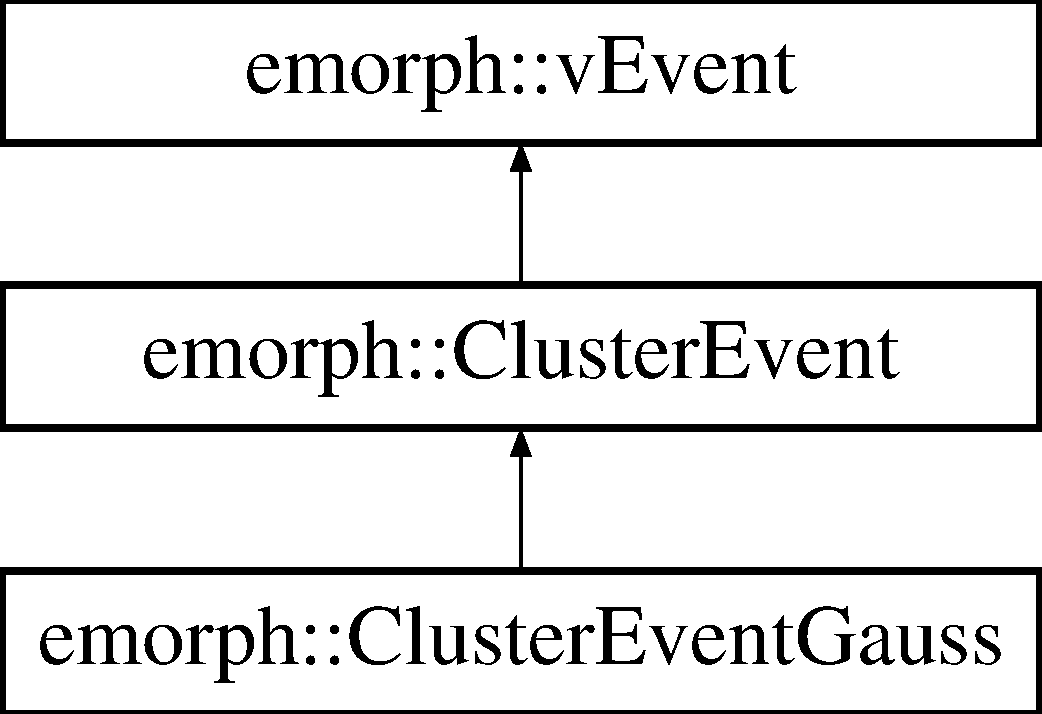
\includegraphics[height=3.000000cm]{classemorph_1_1ClusterEventGauss}
\end{center}
\end{figure}
\subsection*{Public Member Functions}
\begin{DoxyCompactItemize}
\item 
\hypertarget{classemorph_1_1ClusterEventGauss_ab1466fa3a9ed87b9a25d5750892a5537}{virtual std\-::string {\bfseries get\-Type} () const }\label{classemorph_1_1ClusterEventGauss_ab1466fa3a9ed87b9a25d5750892a5537}

\item 
\hypertarget{classemorph_1_1ClusterEventGauss_a1d18b3a9464bf75d9148f7ff519d989d}{int {\bfseries get\-Num\-A\-E} () const }\label{classemorph_1_1ClusterEventGauss_a1d18b3a9464bf75d9148f7ff519d989d}

\item 
\hypertarget{classemorph_1_1ClusterEventGauss_ae1b22b41f455304d09b910cf8c15a891}{int {\bfseries get\-X\-Sigma2} () const }\label{classemorph_1_1ClusterEventGauss_ae1b22b41f455304d09b910cf8c15a891}

\item 
\hypertarget{classemorph_1_1ClusterEventGauss_a1f039476dd020ce632de5d23ecef3622}{int {\bfseries get\-Y\-Sigma2} () const }\label{classemorph_1_1ClusterEventGauss_a1f039476dd020ce632de5d23ecef3622}

\item 
\hypertarget{classemorph_1_1ClusterEventGauss_abb3fe44f71a7231932eec634bab3d754}{int {\bfseries get\-X\-Y\-Sigma} () const }\label{classemorph_1_1ClusterEventGauss_abb3fe44f71a7231932eec634bab3d754}

\item 
\hypertarget{classemorph_1_1ClusterEventGauss_a65fb1212d1216de3d2fb6da9f9594bb2}{int {\bfseries get\-X\-Vel} () const }\label{classemorph_1_1ClusterEventGauss_a65fb1212d1216de3d2fb6da9f9594bb2}

\item 
\hypertarget{classemorph_1_1ClusterEventGauss_ab4cc6e9fc4e72b3eac1d9b2f7d344139}{int {\bfseries get\-Y\-Vel} () const }\label{classemorph_1_1ClusterEventGauss_ab4cc6e9fc4e72b3eac1d9b2f7d344139}

\item 
\hypertarget{classemorph_1_1ClusterEventGauss_a0f7704de0004680899c9a6236a9c7648}{void {\bfseries set\-Num\-A\-E} (const int num\-A\-E)}\label{classemorph_1_1ClusterEventGauss_a0f7704de0004680899c9a6236a9c7648}

\item 
\hypertarget{classemorph_1_1ClusterEventGauss_a4d72be4d66481a18e0f7774d32c129ce}{void {\bfseries set\-X\-Sigma2} (const int x\-Sigma2)}\label{classemorph_1_1ClusterEventGauss_a4d72be4d66481a18e0f7774d32c129ce}

\item 
\hypertarget{classemorph_1_1ClusterEventGauss_a46ee601dff2561697f571776f08a31df}{void {\bfseries set\-Y\-Sigma2} (const int y\-Sigma2)}\label{classemorph_1_1ClusterEventGauss_a46ee601dff2561697f571776f08a31df}

\item 
\hypertarget{classemorph_1_1ClusterEventGauss_aeb562a3c810130f2ed78beee92068d36}{void {\bfseries set\-X\-Y\-Sigma} (const int xy\-Sigma)}\label{classemorph_1_1ClusterEventGauss_aeb562a3c810130f2ed78beee92068d36}

\item 
\hypertarget{classemorph_1_1ClusterEventGauss_a42c68e79097d84b5923f4811a8202a55}{void {\bfseries set\-X\-Vel} (const int x\-Vel)}\label{classemorph_1_1ClusterEventGauss_a42c68e79097d84b5923f4811a8202a55}

\item 
\hypertarget{classemorph_1_1ClusterEventGauss_a791f87f8e52e5eb09d8f1f328ce03819}{void {\bfseries set\-Y\-Vel} (const int y\-Vel)}\label{classemorph_1_1ClusterEventGauss_a791f87f8e52e5eb09d8f1f328ce03819}

\item 
\hypertarget{classemorph_1_1ClusterEventGauss_a47fa9616a54175d33f88b91c60b6d7ef}{{\bfseries Cluster\-Event\-Gauss} (const \hyperlink{classemorph_1_1vEvent}{v\-Event} \&event)}\label{classemorph_1_1ClusterEventGauss_a47fa9616a54175d33f88b91c60b6d7ef}

\item 
\hypertarget{classemorph_1_1ClusterEventGauss_ad192df617898a2c9bade6e522eef17a7}{\hyperlink{classemorph_1_1vEvent}{v\-Event} \& {\bfseries operator=} (const \hyperlink{classemorph_1_1vEvent}{v\-Event} \&event)}\label{classemorph_1_1ClusterEventGauss_ad192df617898a2c9bade6e522eef17a7}

\item 
\hypertarget{classemorph_1_1ClusterEventGauss_acdad728b7929fb9b2f84bf229955bb06}{virtual \hyperlink{classemorph_1_1vEvent}{v\-Event} $\ast$ {\bfseries clone} ()}\label{classemorph_1_1ClusterEventGauss_acdad728b7929fb9b2f84bf229955bb06}

\item 
\hypertarget{classemorph_1_1ClusterEventGauss_a6a6044226e071e01f0ef6270f485d613}{bool {\bfseries operator==} (const \hyperlink{classemorph_1_1ClusterEventGauss}{Cluster\-Event\-Gauss} \&event)}\label{classemorph_1_1ClusterEventGauss_a6a6044226e071e01f0ef6270f485d613}

\item 
\hypertarget{classemorph_1_1ClusterEventGauss_acfc05cadf09c3e4f5331bd2bcf8616c9}{bool {\bfseries operator==} (const \hyperlink{classemorph_1_1vEvent}{v\-Event} \&event)}\label{classemorph_1_1ClusterEventGauss_acfc05cadf09c3e4f5331bd2bcf8616c9}

\item 
\hypertarget{classemorph_1_1ClusterEventGauss_abef5e6b58b3e7ae3200fd623e9110d75}{virtual void {\bfseries encode} (yarp\-::os\-::\-Bottle \&b) const }\label{classemorph_1_1ClusterEventGauss_abef5e6b58b3e7ae3200fd623e9110d75}

\item 
\hypertarget{classemorph_1_1ClusterEventGauss_a2a6a74f6706217b8f75b9562e8f2f320}{yarp\-::os\-::\-Property {\bfseries get\-Content} () const }\label{classemorph_1_1ClusterEventGauss_a2a6a74f6706217b8f75b9562e8f2f320}

\item 
\hypertarget{classemorph_1_1ClusterEventGauss_a0a95ac26ca256bfbd0599b938ef82b5b}{virtual bool {\bfseries decode} (const yarp\-::os\-::\-Bottle \&packet, int \&pos)}\label{classemorph_1_1ClusterEventGauss_a0a95ac26ca256bfbd0599b938ef82b5b}

\item 
\hypertarget{classemorph_1_1ClusterEventGauss_a8cbd43b80dca05d8c6ba6c219fe1f98e}{virtual int {\bfseries n\-Bytes\-Coded} () const }\label{classemorph_1_1ClusterEventGauss_a8cbd43b80dca05d8c6ba6c219fe1f98e}

\end{DoxyCompactItemize}
\subsection*{Protected Attributes}
\begin{DoxyCompactItemize}
\item 
\hypertarget{classemorph_1_1ClusterEventGauss_af3aae4ebf9ad1480bfa69f31510de0ec}{unsigned short int {\bfseries num\-A\-E}}\label{classemorph_1_1ClusterEventGauss_af3aae4ebf9ad1480bfa69f31510de0ec}

\item 
\hypertarget{classemorph_1_1ClusterEventGauss_ab6729a1ffaa8830616a9aca3acbd7f17}{short int {\bfseries xy\-Sigma}}\label{classemorph_1_1ClusterEventGauss_ab6729a1ffaa8830616a9aca3acbd7f17}

\item 
\hypertarget{classemorph_1_1ClusterEventGauss_a6b982b8cfc34739bf96af09ac6374579}{unsigned short int {\bfseries x\-Sigma2}}\label{classemorph_1_1ClusterEventGauss_a6b982b8cfc34739bf96af09ac6374579}

\item 
\hypertarget{classemorph_1_1ClusterEventGauss_a5984b8f2d259c355100414d6240cc5bf}{unsigned short int {\bfseries y\-Sigma2}}\label{classemorph_1_1ClusterEventGauss_a5984b8f2d259c355100414d6240cc5bf}

\item 
\hypertarget{classemorph_1_1ClusterEventGauss_af77be89b7e9efdcc8be716f59b5eae62}{short int {\bfseries x\-Vel}}\label{classemorph_1_1ClusterEventGauss_af77be89b7e9efdcc8be716f59b5eae62}

\item 
\hypertarget{classemorph_1_1ClusterEventGauss_aade9776936f4d390084d4c34c26ef77f}{short int {\bfseries y\-Vel}}\label{classemorph_1_1ClusterEventGauss_aade9776936f4d390084d4c34c26ef77f}

\end{DoxyCompactItemize}
\subsection*{Additional Inherited Members}


The documentation for this class was generated from the following files\-:\begin{DoxyCompactItemize}
\item 
/home/aglover/workspace/projects/event\-Driven/emorph\-\_\-lib/include/i\-Cub/emorph/v\-Codec.\-h\item 
/home/aglover/workspace/projects/event\-Driven/emorph\-\_\-lib/src/v\-Codec.\-cpp\end{DoxyCompactItemize}

\hypertarget{classemorph_1_1CollisionEvent}{\section{emorph\-:\-:Collision\-Event Class Reference}
\label{classemorph_1_1CollisionEvent}\index{emorph\-::\-Collision\-Event@{emorph\-::\-Collision\-Event}}
}
Inheritance diagram for emorph\-:\-:Collision\-Event\-:\begin{figure}[H]
\begin{center}
\leavevmode
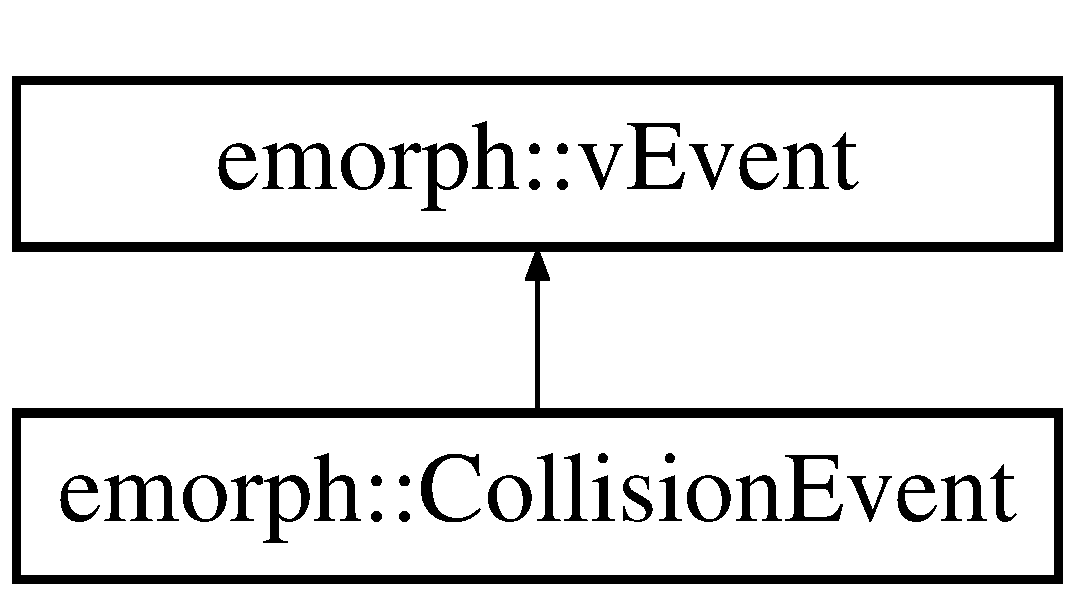
\includegraphics[height=2.000000cm]{classemorph_1_1CollisionEvent}
\end{center}
\end{figure}
\subsection*{Public Member Functions}
\begin{DoxyCompactItemize}
\item 
\hypertarget{classemorph_1_1CollisionEvent_a2da76f2bb1ce603a50221228b2465bf5}{virtual std\-::string {\bfseries get\-Type} () const }\label{classemorph_1_1CollisionEvent_a2da76f2bb1ce603a50221228b2465bf5}

\item 
\hypertarget{classemorph_1_1CollisionEvent_a167522df5c67b6156235e99ff636682a}{void {\bfseries set\-X} (unsigned char x)}\label{classemorph_1_1CollisionEvent_a167522df5c67b6156235e99ff636682a}

\item 
\hypertarget{classemorph_1_1CollisionEvent_a0ee83443e28c0acfc221851192386fa4}{void {\bfseries set\-Y} (unsigned char y)}\label{classemorph_1_1CollisionEvent_a0ee83443e28c0acfc221851192386fa4}

\item 
\hypertarget{classemorph_1_1CollisionEvent_a574b19f46b81c78ce52b14027a5b7a02}{void {\bfseries set\-Channel} (unsigned char channel)}\label{classemorph_1_1CollisionEvent_a574b19f46b81c78ce52b14027a5b7a02}

\item 
\hypertarget{classemorph_1_1CollisionEvent_a6b573077944ecf238c85c1f963bda3ba}{void {\bfseries set\-Clid1} (unsigned char clid1)}\label{classemorph_1_1CollisionEvent_a6b573077944ecf238c85c1f963bda3ba}

\item 
\hypertarget{classemorph_1_1CollisionEvent_a95f28c93a0e7766bae5c179ec86761de}{void {\bfseries set\-Clid2} (unsigned char clid2)}\label{classemorph_1_1CollisionEvent_a95f28c93a0e7766bae5c179ec86761de}

\item 
\hypertarget{classemorph_1_1CollisionEvent_a94096519704b6390649a9e58e74df3fd}{unsigned char {\bfseries get\-X} ()}\label{classemorph_1_1CollisionEvent_a94096519704b6390649a9e58e74df3fd}

\item 
\hypertarget{classemorph_1_1CollisionEvent_a5115fb53d33275f30f39655bdc5de100}{unsigned char {\bfseries get\-Y} ()}\label{classemorph_1_1CollisionEvent_a5115fb53d33275f30f39655bdc5de100}

\item 
\hypertarget{classemorph_1_1CollisionEvent_a7041563ffa86c57f5570b059d6e1b371}{virtual int {\bfseries get\-Channel} ()}\label{classemorph_1_1CollisionEvent_a7041563ffa86c57f5570b059d6e1b371}

\item 
\hypertarget{classemorph_1_1CollisionEvent_a4117e252c0590f2334eafa6b6e2f9e82}{unsigned char {\bfseries get\-Clid1} ()}\label{classemorph_1_1CollisionEvent_a4117e252c0590f2334eafa6b6e2f9e82}

\item 
\hypertarget{classemorph_1_1CollisionEvent_ae190c5d9acd1f99a0341f700e158b80c}{unsigned char {\bfseries get\-Clid2} ()}\label{classemorph_1_1CollisionEvent_ae190c5d9acd1f99a0341f700e158b80c}

\item 
\hypertarget{classemorph_1_1CollisionEvent_aa4876cbc9ede7c5c244d05bc604a68dc}{{\bfseries Collision\-Event} (const \hyperlink{classemorph_1_1vEvent}{v\-Event} \&event)}\label{classemorph_1_1CollisionEvent_aa4876cbc9ede7c5c244d05bc604a68dc}

\item 
\hypertarget{classemorph_1_1CollisionEvent_aaa148216ab002140d270f19619ba881a}{\hyperlink{classemorph_1_1vEvent}{v\-Event} \& {\bfseries operator=} (const \hyperlink{classemorph_1_1vEvent}{v\-Event} \&event)}\label{classemorph_1_1CollisionEvent_aaa148216ab002140d270f19619ba881a}

\item 
\hypertarget{classemorph_1_1CollisionEvent_ab6faba3e78605cff2e136e25a9276355}{virtual \hyperlink{classemorph_1_1vEvent}{v\-Event} $\ast$ {\bfseries clone} ()}\label{classemorph_1_1CollisionEvent_ab6faba3e78605cff2e136e25a9276355}

\item 
\hypertarget{classemorph_1_1CollisionEvent_a9d34222d2183428221aebca15fb6db3b}{bool {\bfseries operator==} (const \hyperlink{classemorph_1_1CollisionEvent}{Collision\-Event} \&event)}\label{classemorph_1_1CollisionEvent_a9d34222d2183428221aebca15fb6db3b}

\item 
\hypertarget{classemorph_1_1CollisionEvent_a12fd7776267aaa057d4370b6a3936669}{bool {\bfseries operator==} (const \hyperlink{classemorph_1_1vEvent}{v\-Event} \&event)}\label{classemorph_1_1CollisionEvent_a12fd7776267aaa057d4370b6a3936669}

\item 
\hypertarget{classemorph_1_1CollisionEvent_a6f55d79771ccfd4dc87da74e0419da6a}{virtual void {\bfseries encode} (yarp\-::os\-::\-Bottle \&b) const }\label{classemorph_1_1CollisionEvent_a6f55d79771ccfd4dc87da74e0419da6a}

\item 
\hypertarget{classemorph_1_1CollisionEvent_adb201a465b533d2fc0aef13584841553}{yarp\-::os\-::\-Property {\bfseries get\-Content} () const }\label{classemorph_1_1CollisionEvent_adb201a465b533d2fc0aef13584841553}

\item 
\hypertarget{classemorph_1_1CollisionEvent_acf7bde166ff6c125b8df85a25b027282}{virtual bool {\bfseries decode} (const yarp\-::os\-::\-Bottle \&packet, int \&pos)}\label{classemorph_1_1CollisionEvent_acf7bde166ff6c125b8df85a25b027282}

\item 
\hypertarget{classemorph_1_1CollisionEvent_a442efa9c52a54074ab843edc9b8bbb57}{virtual int {\bfseries n\-Bytes\-Coded} () const }\label{classemorph_1_1CollisionEvent_a442efa9c52a54074ab843edc9b8bbb57}

\end{DoxyCompactItemize}
\subsection*{Protected Attributes}
\begin{DoxyCompactItemize}
\item 
\hypertarget{classemorph_1_1CollisionEvent_a67f17bca7d5c16526a87cbb7a7962498}{unsigned char {\bfseries x}}\label{classemorph_1_1CollisionEvent_a67f17bca7d5c16526a87cbb7a7962498}

\item 
\hypertarget{classemorph_1_1CollisionEvent_aa586cf783684799338ab52ff4414dff6}{unsigned char {\bfseries y}}\label{classemorph_1_1CollisionEvent_aa586cf783684799338ab52ff4414dff6}

\item 
\hypertarget{classemorph_1_1CollisionEvent_a1d469ac4d1a0d4c403eea66ce10789d2}{char {\bfseries channel}}\label{classemorph_1_1CollisionEvent_a1d469ac4d1a0d4c403eea66ce10789d2}

\item 
\hypertarget{classemorph_1_1CollisionEvent_a35a3cbb65dfc24190c0bc7bd9d4dad89}{unsigned char {\bfseries clid1}}\label{classemorph_1_1CollisionEvent_a35a3cbb65dfc24190c0bc7bd9d4dad89}

\item 
\hypertarget{classemorph_1_1CollisionEvent_a4742ecacfb76e1f5be614d6c8c7a102b}{unsigned char {\bfseries clid2}}\label{classemorph_1_1CollisionEvent_a4742ecacfb76e1f5be614d6c8c7a102b}

\end{DoxyCompactItemize}
\subsection*{Additional Inherited Members}


The documentation for this class was generated from the following files\-:\begin{DoxyCompactItemize}
\item 
/home/aglover/workspace/projects/event\-Driven/emorph\-\_\-lib/include/i\-Cub/emorph/v\-Codec.\-h\item 
/home/aglover/workspace/projects/event\-Driven/emorph\-\_\-lib/src/v\-Codec.\-cpp\end{DoxyCompactItemize}

\hypertarget{classdevice2yarp}{\section{device2yarp Class Reference}
\label{classdevice2yarp}\index{device2yarp@{device2yarp}}
}
Inheritance diagram for device2yarp\-:\begin{figure}[H]
\begin{center}
\leavevmode
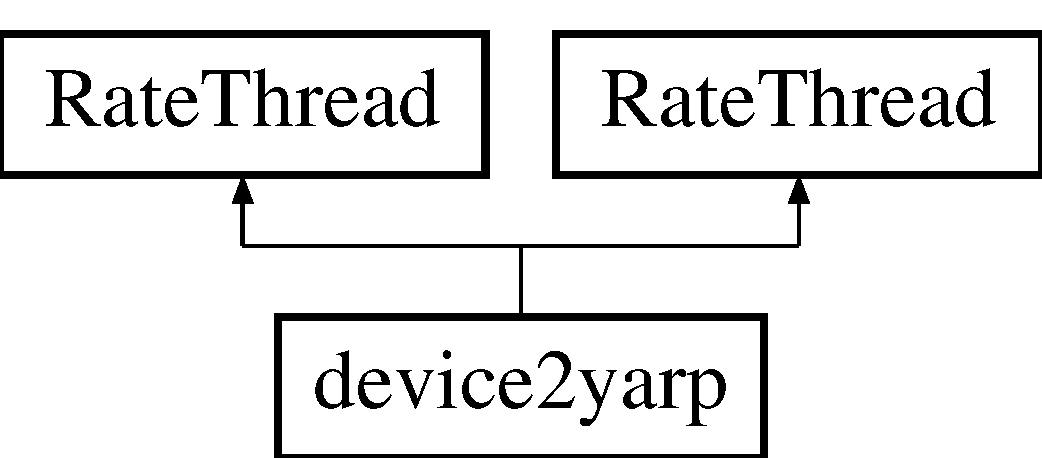
\includegraphics[height=2.000000cm]{classdevice2yarp}
\end{center}
\end{figure}
\subsection*{Public Member Functions}
\begin{DoxyCompactItemize}
\item 
\hypertarget{classdevice2yarp_a2871ae4aafa163197e3991486d3c8b18}{{\bfseries device2yarp} (std\-::string device\-Number, bool save, std\-::string filename)}\label{classdevice2yarp_a2871ae4aafa163197e3991486d3c8b18}

\item 
\hypertarget{classdevice2yarp_aa01eb91fc90a62cb29df3fdc8387cb54}{virtual void {\bfseries run} ()}\label{classdevice2yarp_aa01eb91fc90a62cb29df3fdc8387cb54}

\item 
\hypertarget{classdevice2yarp_ae429ee3f9ab68ceea96daf63553e7700}{virtual void {\bfseries thread\-Release} ()}\label{classdevice2yarp_ae429ee3f9ab68ceea96daf63553e7700}

\item 
void \hyperlink{classdevice2yarp_afbcd3cc36aeda39c389037ff480a0c3a}{prepare\-Biases} ()
\item 
void \hyperlink{classdevice2yarp_ab103ad6beed47415371ec71cc2ac30c3}{prepare\-Biases\-Right} ()
\item 
void \hyperlink{classdevice2yarp_aaaff6edb1a3d7830d6e87b14226e9207}{set\-Device\-Name} (std\-::string name)
\item 
void \hyperlink{classdevice2yarp_af60c47d12785c8bbc8ffb0a29f740a97}{close\-Device} ()
\item 
void \hyperlink{classdevice2yarp_a2ad1d6367e70bbc19d163b80a959843b}{prog\-Bias} (std\-::string name, int bits, int value, int camera=1)
\item 
void \hyperlink{classdevice2yarp_a148575c0588c481968e8e1c89aa1b2d8}{latch\-Commit} (int camera=1)
\item 
void \hyperlink{classdevice2yarp_ad5db8d09f97eb010e8037de3aafe4c0c}{latch\-Commit\-A\-Es} (int camera=1)
\item 
void \hyperlink{classdevice2yarp_a5227cd9f8f77fc3282abdb4f067c72db}{reset\-Pins} (int camera=1)
\item 
void \hyperlink{classdevice2yarp_acd91e6286807878481a293929579a358}{release\-Powerdown} (int camera=1)
\item 
void \hyperlink{classdevice2yarp_a468ec9658d04b2c89ea383a398245279}{set\-Powerdown} (int camera=1)
\item 
void \hyperlink{classdevice2yarp_a65726cde64ea739945753f5b51e84d8b}{prog\-Bit} (int bitvalue, int camera=1)
\item 
void \hyperlink{classdevice2yarp_a5291edc3d845bc6dd35c6d1a783ea80c}{prog\-Bit\-A\-Es} (int bitvalue, int camera=1)
\item 
void \hyperlink{classdevice2yarp_a39c03e4a4e0ac4b891947b872974f8af}{biasprogtx} (int time, int latch, int clock, int data, int powerdown=1, int camera=1)
\item 
void \hyperlink{classdevice2yarp_a19c60dd42e00da0e717da9fe17a5b2f5}{monitor} (int secs, int camera=1)
\item 
void \hyperlink{classdevice2yarp_a300aab882d64fa1a51b2058b530c8093}{sending\-Bias} ()
\item 
void \hyperlink{classdevice2yarp_a704565be367fa28840df912a97bdc25a}{set\-Only\-Left} ()
\item 
void \hyperlink{classdevice2yarp_a94653e9e8ce5ac4a60ae920f0ee41ee6}{set\-From\-Binary} (bool value)
\item 
void \hyperlink{classdevice2yarp_a1982c1021d9e51c789dfc5369dcb46bf}{set\-Binary\-File} (F\-I\-L\-E $\ast$f)
\item 
void \hyperlink{classdevice2yarp_a88ab89295bfefefbc9ac225dd5078dec}{set\-P\-R} (double value)
\item 
void \hyperlink{classdevice2yarp_a96f85845d4902b017e7d082cbc736735}{set\-F\-O\-L\-L} (double value)
\item 
void \hyperlink{classdevice2yarp_a813be66e7621e575682f44e92efa20ef}{set\-D\-I\-F\-F} (double value)
\item 
void \hyperlink{classdevice2yarp_ac072c8cf5341ae1bb187eacbaf8bc439}{set\-D\-I\-F\-F\-O\-N} (double value)
\item 
void \hyperlink{classdevice2yarp_a263fc557cd4333c9cff0e9e4a3f283cd}{set\-P\-U\-Y} (double value)
\item 
void \hyperlink{classdevice2yarp_a24d972c0905025758a9d25607feaccf3}{set\-R\-E\-F\-R} (double value)
\item 
void \hyperlink{classdevice2yarp_add886f7ed984d3b47788df4cd294f2bc}{set\-R\-E\-Q} (double value)
\item 
void \hyperlink{classdevice2yarp_a202830f7c13eaff007c2594cc5e1d1ba}{set\-D\-I\-F\-F\-O\-F\-F} (double value)
\item 
void \hyperlink{classdevice2yarp_a1e9703e924441f50217aa4ded2be6c57}{set\-P\-U\-X} (double value)
\item 
void \hyperlink{classdevice2yarp_aea2c1f8287d1f9e95ac1ff2dc5ed878b}{set\-R\-E\-Q\-P\-D} (double value)
\item 
void \hyperlink{classdevice2yarp_afaf4e9eba2aa0d2f08602b7a03c6e5bf}{set\-I\-N\-J\-G\-N\-D} (double value)
\item 
void \hyperlink{classdevice2yarp_a469e0006636382fb25380147e146114f}{set\-C\-A\-S} (double value)
\item 
void \hyperlink{classdevice2yarp_a223f809aba867489a6b95c3b1ff66b15}{set\-P\-R\-Right} (double value)
\item 
void \hyperlink{classdevice2yarp_a27c6f1f15ceed7423118303431c9b54c}{set\-F\-O\-L\-L\-Right} (double value)
\item 
void \hyperlink{classdevice2yarp_add9e9df708995e75461d4589aae966c2}{set\-D\-I\-F\-F\-Right} (double value)
\item 
void \hyperlink{classdevice2yarp_aba1778322dffc46348dd78f0b86e56b0}{set\-D\-I\-F\-F\-O\-N\-Right} (double value)
\item 
void \hyperlink{classdevice2yarp_a0e60d43576b2d8f9c26519d09a14a564}{set\-P\-U\-Y\-Right} (double value)
\item 
void \hyperlink{classdevice2yarp_a026af71fd22a53e87896a1b1e5fbe2d9}{set\-R\-E\-F\-R\-Right} (double value)
\item 
void \hyperlink{classdevice2yarp_acb5c45d2835c3ea311f81daf2f4545cd}{set\-R\-E\-Q\-Right} (double value)
\item 
void \hyperlink{classdevice2yarp_a5a62082f903ae997ee15f3616c332635}{set\-D\-I\-F\-F\-O\-F\-F\-Right} (double value)
\item 
void \hyperlink{classdevice2yarp_a86ac1223c0a74dacebc26597e1a16ae9}{set\-P\-U\-X\-Right} (double value)
\item 
void \hyperlink{classdevice2yarp_aaac082c96f859df902389e60be83c328}{set\-R\-E\-Q\-P\-D\-Right} (double value)
\item 
void \hyperlink{classdevice2yarp_afab1c11e9c891a5b2103afa5d6101374}{set\-I\-N\-J\-G\-N\-D\-Right} (double value)
\item 
void \hyperlink{classdevice2yarp_aaa3573b8c4bb7e0348c97b87ef8edcd2}{set\-C\-A\-S\-Right} (double value)
\item 
void \hyperlink{classdevice2yarp_a4ef67bab52a9bbee2c590960afffc2e3}{set\-Dump\-Event} (bool value)
\item 
bool \hyperlink{classdevice2yarp_ac53bd1cc581717e681ad3ea0962db697}{set\-Dump\-File} (std\-::string value)
\item 
void \hyperlink{classdevice2yarp_ad5c9adf0e41f78d38a1d1b9265011dfa}{set\-Sync\-Bit} ()
\item 
double \hyperlink{classdevice2yarp_a85742caba0c13dbec757e034419ac570}{get\-P\-R} ()
\item 
double \hyperlink{classdevice2yarp_a45256821729711ac676b98fd86a2934b}{get\-F\-O\-L\-L} ()
\item 
double \hyperlink{classdevice2yarp_ac49ff696fd4ca634fb00188c7f84d5e0}{get\-D\-I\-F\-F} ()
\item 
double \hyperlink{classdevice2yarp_ae82c9cacfc6df370b144f764e1ba2d71}{get\-D\-I\-F\-F\-O\-N} ()
\item 
double \hyperlink{classdevice2yarp_a35e0c7313c78f7d4cfe7403b20742be7}{get\-P\-U\-Y} ()
\item 
double \hyperlink{classdevice2yarp_a0cfbc83863780cb22777ea0df0dff4bb}{get\-R\-E\-F\-R} ()
\item 
double \hyperlink{classdevice2yarp_a02f8aaa21afea5a2c3cf690d4a7a810a}{get\-R\-E\-Q} ()
\item 
double \hyperlink{classdevice2yarp_aebb49f54bbbd1f89767ebc7473cf27f8}{get\-D\-I\-F\-F\-O\-F\-F} ()
\item 
double \hyperlink{classdevice2yarp_a17cabe5685326832b143a95bc079fce2}{get\-P\-U\-X} ()
\item 
double \hyperlink{classdevice2yarp_ad9668df280f370362a6be3d020766b53}{get\-R\-E\-Q\-P\-D} ()
\item 
double \hyperlink{classdevice2yarp_a71d866e65c1a1da500cde870fc9a4202}{get\-I\-N\-J\-G\-N\-D} ()
\item 
double \hyperlink{classdevice2yarp_a2695a28ec3a0864fd1f16bf58b757338}{get\-C\-A\-S} ()
\item 
\hypertarget{classdevice2yarp_a2edb15ab91293f60b5ba2426ae247e1e}{virtual void {\bfseries run} ()}\label{classdevice2yarp_a2edb15ab91293f60b5ba2426ae247e1e}

\item 
\hypertarget{classdevice2yarp_a684963ad891d4dc4e19c5128c88bfff0}{virtual void {\bfseries thread\-Release} ()}\label{classdevice2yarp_a684963ad891d4dc4e19c5128c88bfff0}

\item 
\hypertarget{classdevice2yarp_a900e8d97564445ea12e8d11448197f4a}{virtual bool {\bfseries thread\-Init} (std\-::string module\-Name=\char`\"{}\char`\"{})}\label{classdevice2yarp_a900e8d97564445ea12e8d11448197f4a}

\item 
\hypertarget{classdevice2yarp_ad969527a6d59bcfb1be6349a80defa13}{void {\bfseries attach\-Device\-Manager} (\hyperlink{classdeviceManager}{device\-Manager} $\ast$dev\-Manager)}\label{classdevice2yarp_ad969527a6d59bcfb1be6349a80defa13}

\end{DoxyCompactItemize}


\subsection{Member Function Documentation}
\hypertarget{classdevice2yarp_a39c03e4a4e0ac4b891947b872974f8af}{\index{device2yarp@{device2yarp}!biasprogtx@{biasprogtx}}
\index{biasprogtx@{biasprogtx}!device2yarp@{device2yarp}}
\subsubsection[{biasprogtx}]{\setlength{\rightskip}{0pt plus 5cm}void device2yarp\-::biasprogtx (
\begin{DoxyParamCaption}
\item[{int}]{time, }
\item[{int}]{latch, }
\item[{int}]{clock, }
\item[{int}]{data, }
\item[{int}]{powerdown = {\ttfamily 1}, }
\item[{int}]{camera = {\ttfamily 1}}
\end{DoxyParamCaption}
)}}\label{classdevice2yarp_a39c03e4a4e0ac4b891947b872974f8af}
function that send biases to F\-P\-G\-A.\-The F\-P\-G\-A then first waits for the sequencer time to expire as for every other A\-E, then the lowest four bits of the A\-E, R\-I\-G\-H\-T/\-L\-E\-F\-T in 0x\-F\-F0000\-R\-L would be interpreted as new values for the bias programming pins. 
\begin{DoxyParams}{Parameters}
{\em time} & sequence time to expire before programming data \\
\hline
{\em latch} & control of the latch pin \\
\hline
{\em clock} & control of the clock \\
\hline
{\em data} & data that is sent \\
\hline
{\em powerdown} & control of the powerdown \\
\hline
{\em camera} & defines which camera is going to be programmed (Left 1, Right 0) \\
\hline
\end{DoxyParams}
\hypertarget{classdevice2yarp_af60c47d12785c8bbc8ffb0a29f740a97}{\index{device2yarp@{device2yarp}!close\-Device@{close\-Device}}
\index{close\-Device@{close\-Device}!device2yarp@{device2yarp}}
\subsubsection[{close\-Device}]{\setlength{\rightskip}{0pt plus 5cm}void device2yarp\-::close\-Device (
\begin{DoxyParamCaption}
{}
\end{DoxyParamCaption}
)}}\label{classdevice2yarp_af60c47d12785c8bbc8ffb0a29f740a97}
function that correcly closes the device \hypertarget{classdevice2yarp_a2695a28ec3a0864fd1f16bf58b757338}{\index{device2yarp@{device2yarp}!get\-C\-A\-S@{get\-C\-A\-S}}
\index{get\-C\-A\-S@{get\-C\-A\-S}!device2yarp@{device2yarp}}
\subsubsection[{get\-C\-A\-S}]{\setlength{\rightskip}{0pt plus 5cm}double device2yarp\-::get\-C\-A\-S (
\begin{DoxyParamCaption}
{}
\end{DoxyParamCaption}
)\hspace{0.3cm}{\ttfamily [inline]}}}\label{classdevice2yarp_a2695a28ec3a0864fd1f16bf58b757338}
function that returns the bias for Left camera \begin{DoxyReturn}{Returns}
value of the bias 
\end{DoxyReturn}
\hypertarget{classdevice2yarp_ac49ff696fd4ca634fb00188c7f84d5e0}{\index{device2yarp@{device2yarp}!get\-D\-I\-F\-F@{get\-D\-I\-F\-F}}
\index{get\-D\-I\-F\-F@{get\-D\-I\-F\-F}!device2yarp@{device2yarp}}
\subsubsection[{get\-D\-I\-F\-F}]{\setlength{\rightskip}{0pt plus 5cm}double device2yarp\-::get\-D\-I\-F\-F (
\begin{DoxyParamCaption}
{}
\end{DoxyParamCaption}
)\hspace{0.3cm}{\ttfamily [inline]}}}\label{classdevice2yarp_ac49ff696fd4ca634fb00188c7f84d5e0}
function that returns the bias for Left camera \begin{DoxyReturn}{Returns}
value of the bias 
\end{DoxyReturn}
\hypertarget{classdevice2yarp_aebb49f54bbbd1f89767ebc7473cf27f8}{\index{device2yarp@{device2yarp}!get\-D\-I\-F\-F\-O\-F\-F@{get\-D\-I\-F\-F\-O\-F\-F}}
\index{get\-D\-I\-F\-F\-O\-F\-F@{get\-D\-I\-F\-F\-O\-F\-F}!device2yarp@{device2yarp}}
\subsubsection[{get\-D\-I\-F\-F\-O\-F\-F}]{\setlength{\rightskip}{0pt plus 5cm}double device2yarp\-::get\-D\-I\-F\-F\-O\-F\-F (
\begin{DoxyParamCaption}
{}
\end{DoxyParamCaption}
)\hspace{0.3cm}{\ttfamily [inline]}}}\label{classdevice2yarp_aebb49f54bbbd1f89767ebc7473cf27f8}
function that returns the bias for Left camera \begin{DoxyReturn}{Returns}
value of the bias 
\end{DoxyReturn}
\hypertarget{classdevice2yarp_ae82c9cacfc6df370b144f764e1ba2d71}{\index{device2yarp@{device2yarp}!get\-D\-I\-F\-F\-O\-N@{get\-D\-I\-F\-F\-O\-N}}
\index{get\-D\-I\-F\-F\-O\-N@{get\-D\-I\-F\-F\-O\-N}!device2yarp@{device2yarp}}
\subsubsection[{get\-D\-I\-F\-F\-O\-N}]{\setlength{\rightskip}{0pt plus 5cm}double device2yarp\-::get\-D\-I\-F\-F\-O\-N (
\begin{DoxyParamCaption}
{}
\end{DoxyParamCaption}
)\hspace{0.3cm}{\ttfamily [inline]}}}\label{classdevice2yarp_ae82c9cacfc6df370b144f764e1ba2d71}
function that returns the bias for Left camera \begin{DoxyReturn}{Returns}
value of the bias 
\end{DoxyReturn}
\hypertarget{classdevice2yarp_a45256821729711ac676b98fd86a2934b}{\index{device2yarp@{device2yarp}!get\-F\-O\-L\-L@{get\-F\-O\-L\-L}}
\index{get\-F\-O\-L\-L@{get\-F\-O\-L\-L}!device2yarp@{device2yarp}}
\subsubsection[{get\-F\-O\-L\-L}]{\setlength{\rightskip}{0pt plus 5cm}double device2yarp\-::get\-F\-O\-L\-L (
\begin{DoxyParamCaption}
{}
\end{DoxyParamCaption}
)\hspace{0.3cm}{\ttfamily [inline]}}}\label{classdevice2yarp_a45256821729711ac676b98fd86a2934b}
function that returns the bias for Left camera \begin{DoxyReturn}{Returns}
value of the bias 
\end{DoxyReturn}
\hypertarget{classdevice2yarp_a71d866e65c1a1da500cde870fc9a4202}{\index{device2yarp@{device2yarp}!get\-I\-N\-J\-G\-N\-D@{get\-I\-N\-J\-G\-N\-D}}
\index{get\-I\-N\-J\-G\-N\-D@{get\-I\-N\-J\-G\-N\-D}!device2yarp@{device2yarp}}
\subsubsection[{get\-I\-N\-J\-G\-N\-D}]{\setlength{\rightskip}{0pt plus 5cm}double device2yarp\-::get\-I\-N\-J\-G\-N\-D (
\begin{DoxyParamCaption}
{}
\end{DoxyParamCaption}
)\hspace{0.3cm}{\ttfamily [inline]}}}\label{classdevice2yarp_a71d866e65c1a1da500cde870fc9a4202}
function that returns the bias for Left camera \begin{DoxyReturn}{Returns}
value of the bias 
\end{DoxyReturn}
\hypertarget{classdevice2yarp_a85742caba0c13dbec757e034419ac570}{\index{device2yarp@{device2yarp}!get\-P\-R@{get\-P\-R}}
\index{get\-P\-R@{get\-P\-R}!device2yarp@{device2yarp}}
\subsubsection[{get\-P\-R}]{\setlength{\rightskip}{0pt plus 5cm}double device2yarp\-::get\-P\-R (
\begin{DoxyParamCaption}
{}
\end{DoxyParamCaption}
)\hspace{0.3cm}{\ttfamily [inline]}}}\label{classdevice2yarp_a85742caba0c13dbec757e034419ac570}
function that returns the bias for Left camera \begin{DoxyReturn}{Returns}
value of the bias 
\end{DoxyReturn}
\hypertarget{classdevice2yarp_a17cabe5685326832b143a95bc079fce2}{\index{device2yarp@{device2yarp}!get\-P\-U\-X@{get\-P\-U\-X}}
\index{get\-P\-U\-X@{get\-P\-U\-X}!device2yarp@{device2yarp}}
\subsubsection[{get\-P\-U\-X}]{\setlength{\rightskip}{0pt plus 5cm}double device2yarp\-::get\-P\-U\-X (
\begin{DoxyParamCaption}
{}
\end{DoxyParamCaption}
)\hspace{0.3cm}{\ttfamily [inline]}}}\label{classdevice2yarp_a17cabe5685326832b143a95bc079fce2}
function that returns the bias for Left camera \begin{DoxyReturn}{Returns}
value of the bias 
\end{DoxyReturn}
\hypertarget{classdevice2yarp_a35e0c7313c78f7d4cfe7403b20742be7}{\index{device2yarp@{device2yarp}!get\-P\-U\-Y@{get\-P\-U\-Y}}
\index{get\-P\-U\-Y@{get\-P\-U\-Y}!device2yarp@{device2yarp}}
\subsubsection[{get\-P\-U\-Y}]{\setlength{\rightskip}{0pt plus 5cm}double device2yarp\-::get\-P\-U\-Y (
\begin{DoxyParamCaption}
{}
\end{DoxyParamCaption}
)\hspace{0.3cm}{\ttfamily [inline]}}}\label{classdevice2yarp_a35e0c7313c78f7d4cfe7403b20742be7}
function that returns the bias for Left camera \begin{DoxyReturn}{Returns}
value of the bias 
\end{DoxyReturn}
\hypertarget{classdevice2yarp_a0cfbc83863780cb22777ea0df0dff4bb}{\index{device2yarp@{device2yarp}!get\-R\-E\-F\-R@{get\-R\-E\-F\-R}}
\index{get\-R\-E\-F\-R@{get\-R\-E\-F\-R}!device2yarp@{device2yarp}}
\subsubsection[{get\-R\-E\-F\-R}]{\setlength{\rightskip}{0pt plus 5cm}double device2yarp\-::get\-R\-E\-F\-R (
\begin{DoxyParamCaption}
{}
\end{DoxyParamCaption}
)\hspace{0.3cm}{\ttfamily [inline]}}}\label{classdevice2yarp_a0cfbc83863780cb22777ea0df0dff4bb}
function that returns the bias for Left camera \begin{DoxyReturn}{Returns}
value of the bias 
\end{DoxyReturn}
\hypertarget{classdevice2yarp_a02f8aaa21afea5a2c3cf690d4a7a810a}{\index{device2yarp@{device2yarp}!get\-R\-E\-Q@{get\-R\-E\-Q}}
\index{get\-R\-E\-Q@{get\-R\-E\-Q}!device2yarp@{device2yarp}}
\subsubsection[{get\-R\-E\-Q}]{\setlength{\rightskip}{0pt plus 5cm}double device2yarp\-::get\-R\-E\-Q (
\begin{DoxyParamCaption}
{}
\end{DoxyParamCaption}
)\hspace{0.3cm}{\ttfamily [inline]}}}\label{classdevice2yarp_a02f8aaa21afea5a2c3cf690d4a7a810a}
function that returns the bias for Left camera \begin{DoxyReturn}{Returns}
value of the bias 
\end{DoxyReturn}
\hypertarget{classdevice2yarp_ad9668df280f370362a6be3d020766b53}{\index{device2yarp@{device2yarp}!get\-R\-E\-Q\-P\-D@{get\-R\-E\-Q\-P\-D}}
\index{get\-R\-E\-Q\-P\-D@{get\-R\-E\-Q\-P\-D}!device2yarp@{device2yarp}}
\subsubsection[{get\-R\-E\-Q\-P\-D}]{\setlength{\rightskip}{0pt plus 5cm}double device2yarp\-::get\-R\-E\-Q\-P\-D (
\begin{DoxyParamCaption}
{}
\end{DoxyParamCaption}
)\hspace{0.3cm}{\ttfamily [inline]}}}\label{classdevice2yarp_ad9668df280f370362a6be3d020766b53}
function that returns the bias for Left camera \begin{DoxyReturn}{Returns}
value of the bias 
\end{DoxyReturn}
\hypertarget{classdevice2yarp_a148575c0588c481968e8e1c89aa1b2d8}{\index{device2yarp@{device2yarp}!latch\-Commit@{latch\-Commit}}
\index{latch\-Commit@{latch\-Commit}!device2yarp@{device2yarp}}
\subsubsection[{latch\-Commit}]{\setlength{\rightskip}{0pt plus 5cm}void device2yarp\-::latch\-Commit (
\begin{DoxyParamCaption}
\item[{int}]{camera = {\ttfamily 1}}
\end{DoxyParamCaption}
)}}\label{classdevice2yarp_a148575c0588c481968e8e1c89aa1b2d8}
function used to append to a list of bits necessary to send the latch commit  reference to the camera (left 1, right 0) \hypertarget{classdevice2yarp_ad5db8d09f97eb010e8037de3aafe4c0c}{\index{device2yarp@{device2yarp}!latch\-Commit\-A\-Es@{latch\-Commit\-A\-Es}}
\index{latch\-Commit\-A\-Es@{latch\-Commit\-A\-Es}!device2yarp@{device2yarp}}
\subsubsection[{latch\-Commit\-A\-Es}]{\setlength{\rightskip}{0pt plus 5cm}void device2yarp\-::latch\-Commit\-A\-Es (
\begin{DoxyParamCaption}
\item[{int}]{camera = {\ttfamily 1}}
\end{DoxyParamCaption}
)}}\label{classdevice2yarp_ad5db8d09f97eb010e8037de3aafe4c0c}
function used to append to a list of bits necessary to send the latch commit (version 2)  reference to the camera (left 1, right 0) \hypertarget{classdevice2yarp_a19c60dd42e00da0e717da9fe17a5b2f5}{\index{device2yarp@{device2yarp}!monitor@{monitor}}
\index{monitor@{monitor}!device2yarp@{device2yarp}}
\subsubsection[{monitor}]{\setlength{\rightskip}{0pt plus 5cm}void device2yarp\-::monitor (
\begin{DoxyParamCaption}
\item[{int}]{secs, }
\item[{int}]{camera = {\ttfamily 1}}
\end{DoxyParamCaption}
)}}\label{classdevice2yarp_a19c60dd42e00da0e717da9fe17a5b2f5}
function that monitors the output for seconds 
\begin{DoxyParams}{Parameters}
{\em secs} & number of seconds to wait  reference to the camera (left 1, right 0) \\
\hline
\end{DoxyParams}
\hypertarget{classdevice2yarp_afbcd3cc36aeda39c389037ff480a0c3a}{\index{device2yarp@{device2yarp}!prepare\-Biases@{prepare\-Biases}}
\index{prepare\-Biases@{prepare\-Biases}!device2yarp@{device2yarp}}
\subsubsection[{prepare\-Biases}]{\setlength{\rightskip}{0pt plus 5cm}void device2yarp\-::prepare\-Biases (
\begin{DoxyParamCaption}
{}
\end{DoxyParamCaption}
)}}\label{classdevice2yarp_afbcd3cc36aeda39c389037ff480a0c3a}
function that prepares biases either reading them from file or reading the default value \hypertarget{classdevice2yarp_ab103ad6beed47415371ec71cc2ac30c3}{\index{device2yarp@{device2yarp}!prepare\-Biases\-Right@{prepare\-Biases\-Right}}
\index{prepare\-Biases\-Right@{prepare\-Biases\-Right}!device2yarp@{device2yarp}}
\subsubsection[{prepare\-Biases\-Right}]{\setlength{\rightskip}{0pt plus 5cm}void device2yarp\-::prepare\-Biases\-Right (
\begin{DoxyParamCaption}
{}
\end{DoxyParamCaption}
)}}\label{classdevice2yarp_ab103ad6beed47415371ec71cc2ac30c3}
function that prepares biases either reading them from file or reading the default value \hypertarget{classdevice2yarp_a2ad1d6367e70bbc19d163b80a959843b}{\index{device2yarp@{device2yarp}!prog\-Bias@{prog\-Bias}}
\index{prog\-Bias@{prog\-Bias}!device2yarp@{device2yarp}}
\subsubsection[{prog\-Bias}]{\setlength{\rightskip}{0pt plus 5cm}void device2yarp\-::prog\-Bias (
\begin{DoxyParamCaption}
\item[{std\-::string}]{name, }
\item[{int}]{bits, }
\item[{int}]{value, }
\item[{int}]{camera = {\ttfamily 1}}
\end{DoxyParamCaption}
)}}\label{classdevice2yarp_a2ad1d6367e70bbc19d163b80a959843b}
function used to append to a list of commands every single bit necessary to program bias 
\begin{DoxyParams}{Parameters}
{\em name} & name of the bias to be set \\
\hline
{\em bits} & data of the programming \\
\hline
{\em value} & value of the programming  reference to the camera (left 1, right 0) \\
\hline
\end{DoxyParams}
\hypertarget{classdevice2yarp_a65726cde64ea739945753f5b51e84d8b}{\index{device2yarp@{device2yarp}!prog\-Bit@{prog\-Bit}}
\index{prog\-Bit@{prog\-Bit}!device2yarp@{device2yarp}}
\subsubsection[{prog\-Bit}]{\setlength{\rightskip}{0pt plus 5cm}void device2yarp\-::prog\-Bit (
\begin{DoxyParamCaption}
\item[{int}]{bitvalue, }
\item[{int}]{camera = {\ttfamily 1}}
\end{DoxyParamCaption}
)}}\label{classdevice2yarp_a65726cde64ea739945753f5b51e84d8b}
correct sequence of signals necessary to program a bit 
\begin{DoxyParams}{Parameters}
{\em bitvalue} & value of the bit to be programmed  reference to the camera (left 1, right 0) \\
\hline
\end{DoxyParams}
\hypertarget{classdevice2yarp_a5291edc3d845bc6dd35c6d1a783ea80c}{\index{device2yarp@{device2yarp}!prog\-Bit\-A\-Es@{prog\-Bit\-A\-Es}}
\index{prog\-Bit\-A\-Es@{prog\-Bit\-A\-Es}!device2yarp@{device2yarp}}
\subsubsection[{prog\-Bit\-A\-Es}]{\setlength{\rightskip}{0pt plus 5cm}void device2yarp\-::prog\-Bit\-A\-Es (
\begin{DoxyParamCaption}
\item[{int}]{bitvalue, }
\item[{int}]{camera = {\ttfamily 1}}
\end{DoxyParamCaption}
)}}\label{classdevice2yarp_a5291edc3d845bc6dd35c6d1a783ea80c}
correct sequence of signals necessary to program a bit (version 2) 
\begin{DoxyParams}{Parameters}
{\em bitvalue} & value of the bit to be programmed  reference to the camera (left 1, right 0) \\
\hline
\end{DoxyParams}
\hypertarget{classdevice2yarp_acd91e6286807878481a293929579a358}{\index{device2yarp@{device2yarp}!release\-Powerdown@{release\-Powerdown}}
\index{release\-Powerdown@{release\-Powerdown}!device2yarp@{device2yarp}}
\subsubsection[{release\-Powerdown}]{\setlength{\rightskip}{0pt plus 5cm}void device2yarp\-::release\-Powerdown (
\begin{DoxyParamCaption}
\item[{int}]{camera = {\ttfamily 1}}
\end{DoxyParamCaption}
)}}\label{classdevice2yarp_acd91e6286807878481a293929579a358}
function that sends the powerdown to the correct value after the biases have been programmed  reference to the camera (left 1, right 0) \hypertarget{classdevice2yarp_a5227cd9f8f77fc3282abdb4f067c72db}{\index{device2yarp@{device2yarp}!reset\-Pins@{reset\-Pins}}
\index{reset\-Pins@{reset\-Pins}!device2yarp@{device2yarp}}
\subsubsection[{reset\-Pins}]{\setlength{\rightskip}{0pt plus 5cm}void device2yarp\-::reset\-Pins (
\begin{DoxyParamCaption}
\item[{int}]{camera = {\ttfamily 1}}
\end{DoxyParamCaption}
)}}\label{classdevice2yarp_a5227cd9f8f77fc3282abdb4f067c72db}
function used to reset the device to default after a bias is sent  reference to the camera (left 1, right 0) \hypertarget{classdevice2yarp_a300aab882d64fa1a51b2058b530c8093}{\index{device2yarp@{device2yarp}!sending\-Bias@{sending\-Bias}}
\index{sending\-Bias@{sending\-Bias}!device2yarp@{device2yarp}}
\subsubsection[{sending\-Bias}]{\setlength{\rightskip}{0pt plus 5cm}void device2yarp\-::sending\-Bias (
\begin{DoxyParamCaption}
{}
\end{DoxyParamCaption}
)}}\label{classdevice2yarp_a300aab882d64fa1a51b2058b530c8093}
fuction that connects to the device and write the sequence of signals to the device F\-P\-G\-A no matter what camera has been set the biases go to the board \hypertarget{classdevice2yarp_a1982c1021d9e51c789dfc5369dcb46bf}{\index{device2yarp@{device2yarp}!set\-Binary\-File@{set\-Binary\-File}}
\index{set\-Binary\-File@{set\-Binary\-File}!device2yarp@{device2yarp}}
\subsubsection[{set\-Binary\-File}]{\setlength{\rightskip}{0pt plus 5cm}void device2yarp\-::set\-Binary\-File (
\begin{DoxyParamCaption}
\item[{F\-I\-L\-E $\ast$}]{f}
\end{DoxyParamCaption}
)\hspace{0.3cm}{\ttfamily [inline]}}}\label{classdevice2yarp_a1982c1021d9e51c789dfc5369dcb46bf}
function that sets the reference of the input binary file 
\begin{DoxyParams}{Parameters}
{\em f} & pointer to the F\-I\-L\-E of the binary \\
\hline
\end{DoxyParams}
\hypertarget{classdevice2yarp_a469e0006636382fb25380147e146114f}{\index{device2yarp@{device2yarp}!set\-C\-A\-S@{set\-C\-A\-S}}
\index{set\-C\-A\-S@{set\-C\-A\-S}!device2yarp@{device2yarp}}
\subsubsection[{set\-C\-A\-S}]{\setlength{\rightskip}{0pt plus 5cm}void device2yarp\-::set\-C\-A\-S (
\begin{DoxyParamCaption}
\item[{double}]{value}
\end{DoxyParamCaption}
)\hspace{0.3cm}{\ttfamily [inline]}}}\label{classdevice2yarp_a469e0006636382fb25380147e146114f}
function that sets the bias 
\begin{DoxyParams}{Parameters}
{\em value} & value of the bias \\
\hline
\end{DoxyParams}
\hypertarget{classdevice2yarp_aaa3573b8c4bb7e0348c97b87ef8edcd2}{\index{device2yarp@{device2yarp}!set\-C\-A\-S\-Right@{set\-C\-A\-S\-Right}}
\index{set\-C\-A\-S\-Right@{set\-C\-A\-S\-Right}!device2yarp@{device2yarp}}
\subsubsection[{set\-C\-A\-S\-Right}]{\setlength{\rightskip}{0pt plus 5cm}void device2yarp\-::set\-C\-A\-S\-Right (
\begin{DoxyParamCaption}
\item[{double}]{value}
\end{DoxyParamCaption}
)\hspace{0.3cm}{\ttfamily [inline]}}}\label{classdevice2yarp_aaa3573b8c4bb7e0348c97b87ef8edcd2}
function that sets the bias Right 
\begin{DoxyParams}{Parameters}
{\em value} & value of the bias \\
\hline
\end{DoxyParams}
\hypertarget{classdevice2yarp_aaaff6edb1a3d7830d6e87b14226e9207}{\index{device2yarp@{device2yarp}!set\-Device\-Name@{set\-Device\-Name}}
\index{set\-Device\-Name@{set\-Device\-Name}!device2yarp@{device2yarp}}
\subsubsection[{set\-Device\-Name}]{\setlength{\rightskip}{0pt plus 5cm}void device2yarp\-::set\-Device\-Name (
\begin{DoxyParamCaption}
\item[{std\-::string}]{name}
\end{DoxyParamCaption}
)}}\label{classdevice2yarp_aaaff6edb1a3d7830d6e87b14226e9207}
function used to set the name of the port device where biases are sent 
\begin{DoxyParams}{Parameters}
{\em name} & name of the port of the device \\
\hline
\end{DoxyParams}
\hypertarget{classdevice2yarp_a813be66e7621e575682f44e92efa20ef}{\index{device2yarp@{device2yarp}!set\-D\-I\-F\-F@{set\-D\-I\-F\-F}}
\index{set\-D\-I\-F\-F@{set\-D\-I\-F\-F}!device2yarp@{device2yarp}}
\subsubsection[{set\-D\-I\-F\-F}]{\setlength{\rightskip}{0pt plus 5cm}void device2yarp\-::set\-D\-I\-F\-F (
\begin{DoxyParamCaption}
\item[{double}]{value}
\end{DoxyParamCaption}
)\hspace{0.3cm}{\ttfamily [inline]}}}\label{classdevice2yarp_a813be66e7621e575682f44e92efa20ef}
function that sets the bias 
\begin{DoxyParams}{Parameters}
{\em value} & value of the bias \\
\hline
\end{DoxyParams}
\hypertarget{classdevice2yarp_a202830f7c13eaff007c2594cc5e1d1ba}{\index{device2yarp@{device2yarp}!set\-D\-I\-F\-F\-O\-F\-F@{set\-D\-I\-F\-F\-O\-F\-F}}
\index{set\-D\-I\-F\-F\-O\-F\-F@{set\-D\-I\-F\-F\-O\-F\-F}!device2yarp@{device2yarp}}
\subsubsection[{set\-D\-I\-F\-F\-O\-F\-F}]{\setlength{\rightskip}{0pt plus 5cm}void device2yarp\-::set\-D\-I\-F\-F\-O\-F\-F (
\begin{DoxyParamCaption}
\item[{double}]{value}
\end{DoxyParamCaption}
)\hspace{0.3cm}{\ttfamily [inline]}}}\label{classdevice2yarp_a202830f7c13eaff007c2594cc5e1d1ba}
function that sets the bias 
\begin{DoxyParams}{Parameters}
{\em value} & value of the bias \\
\hline
\end{DoxyParams}
\hypertarget{classdevice2yarp_a5a62082f903ae997ee15f3616c332635}{\index{device2yarp@{device2yarp}!set\-D\-I\-F\-F\-O\-F\-F\-Right@{set\-D\-I\-F\-F\-O\-F\-F\-Right}}
\index{set\-D\-I\-F\-F\-O\-F\-F\-Right@{set\-D\-I\-F\-F\-O\-F\-F\-Right}!device2yarp@{device2yarp}}
\subsubsection[{set\-D\-I\-F\-F\-O\-F\-F\-Right}]{\setlength{\rightskip}{0pt plus 5cm}void device2yarp\-::set\-D\-I\-F\-F\-O\-F\-F\-Right (
\begin{DoxyParamCaption}
\item[{double}]{value}
\end{DoxyParamCaption}
)\hspace{0.3cm}{\ttfamily [inline]}}}\label{classdevice2yarp_a5a62082f903ae997ee15f3616c332635}
function that sets the bias Right 
\begin{DoxyParams}{Parameters}
{\em value} & value of the bias \\
\hline
\end{DoxyParams}
\hypertarget{classdevice2yarp_ac072c8cf5341ae1bb187eacbaf8bc439}{\index{device2yarp@{device2yarp}!set\-D\-I\-F\-F\-O\-N@{set\-D\-I\-F\-F\-O\-N}}
\index{set\-D\-I\-F\-F\-O\-N@{set\-D\-I\-F\-F\-O\-N}!device2yarp@{device2yarp}}
\subsubsection[{set\-D\-I\-F\-F\-O\-N}]{\setlength{\rightskip}{0pt plus 5cm}void device2yarp\-::set\-D\-I\-F\-F\-O\-N (
\begin{DoxyParamCaption}
\item[{double}]{value}
\end{DoxyParamCaption}
)\hspace{0.3cm}{\ttfamily [inline]}}}\label{classdevice2yarp_ac072c8cf5341ae1bb187eacbaf8bc439}
function that sets the bias 
\begin{DoxyParams}{Parameters}
{\em value} & value of the bias \\
\hline
\end{DoxyParams}
\hypertarget{classdevice2yarp_aba1778322dffc46348dd78f0b86e56b0}{\index{device2yarp@{device2yarp}!set\-D\-I\-F\-F\-O\-N\-Right@{set\-D\-I\-F\-F\-O\-N\-Right}}
\index{set\-D\-I\-F\-F\-O\-N\-Right@{set\-D\-I\-F\-F\-O\-N\-Right}!device2yarp@{device2yarp}}
\subsubsection[{set\-D\-I\-F\-F\-O\-N\-Right}]{\setlength{\rightskip}{0pt plus 5cm}void device2yarp\-::set\-D\-I\-F\-F\-O\-N\-Right (
\begin{DoxyParamCaption}
\item[{double}]{value}
\end{DoxyParamCaption}
)\hspace{0.3cm}{\ttfamily [inline]}}}\label{classdevice2yarp_aba1778322dffc46348dd78f0b86e56b0}
function that sets the bias Right 
\begin{DoxyParams}{Parameters}
{\em value} & value of the bias \\
\hline
\end{DoxyParams}
\hypertarget{classdevice2yarp_add9e9df708995e75461d4589aae966c2}{\index{device2yarp@{device2yarp}!set\-D\-I\-F\-F\-Right@{set\-D\-I\-F\-F\-Right}}
\index{set\-D\-I\-F\-F\-Right@{set\-D\-I\-F\-F\-Right}!device2yarp@{device2yarp}}
\subsubsection[{set\-D\-I\-F\-F\-Right}]{\setlength{\rightskip}{0pt plus 5cm}void device2yarp\-::set\-D\-I\-F\-F\-Right (
\begin{DoxyParamCaption}
\item[{double}]{value}
\end{DoxyParamCaption}
)\hspace{0.3cm}{\ttfamily [inline]}}}\label{classdevice2yarp_add9e9df708995e75461d4589aae966c2}
function that sets the bias Right 
\begin{DoxyParams}{Parameters}
{\em value} & value of the bias \\
\hline
\end{DoxyParams}
\hypertarget{classdevice2yarp_a4ef67bab52a9bbee2c590960afffc2e3}{\index{device2yarp@{device2yarp}!set\-Dump\-Event@{set\-Dump\-Event}}
\index{set\-Dump\-Event@{set\-Dump\-Event}!device2yarp@{device2yarp}}
\subsubsection[{set\-Dump\-Event}]{\setlength{\rightskip}{0pt plus 5cm}void device2yarp\-::set\-Dump\-Event (
\begin{DoxyParamCaption}
\item[{bool}]{value}
\end{DoxyParamCaption}
)}}\label{classdevice2yarp_a4ef67bab52a9bbee2c590960afffc2e3}
indicates whether the event has to be saved in a file \hypertarget{classdevice2yarp_ac53bd1cc581717e681ad3ea0962db697}{\index{device2yarp@{device2yarp}!set\-Dump\-File@{set\-Dump\-File}}
\index{set\-Dump\-File@{set\-Dump\-File}!device2yarp@{device2yarp}}
\subsubsection[{set\-Dump\-File}]{\setlength{\rightskip}{0pt plus 5cm}bool device2yarp\-::set\-Dump\-File (
\begin{DoxyParamCaption}
\item[{std\-::string}]{value}
\end{DoxyParamCaption}
)}}\label{classdevice2yarp_ac53bd1cc581717e681ad3ea0962db697}
reference to the name of the file where events are dumped \hypertarget{classdevice2yarp_a96f85845d4902b017e7d082cbc736735}{\index{device2yarp@{device2yarp}!set\-F\-O\-L\-L@{set\-F\-O\-L\-L}}
\index{set\-F\-O\-L\-L@{set\-F\-O\-L\-L}!device2yarp@{device2yarp}}
\subsubsection[{set\-F\-O\-L\-L}]{\setlength{\rightskip}{0pt plus 5cm}void device2yarp\-::set\-F\-O\-L\-L (
\begin{DoxyParamCaption}
\item[{double}]{value}
\end{DoxyParamCaption}
)\hspace{0.3cm}{\ttfamily [inline]}}}\label{classdevice2yarp_a96f85845d4902b017e7d082cbc736735}
function that sets the bias 
\begin{DoxyParams}{Parameters}
{\em value} & value of the bias \\
\hline
\end{DoxyParams}
\hypertarget{classdevice2yarp_a27c6f1f15ceed7423118303431c9b54c}{\index{device2yarp@{device2yarp}!set\-F\-O\-L\-L\-Right@{set\-F\-O\-L\-L\-Right}}
\index{set\-F\-O\-L\-L\-Right@{set\-F\-O\-L\-L\-Right}!device2yarp@{device2yarp}}
\subsubsection[{set\-F\-O\-L\-L\-Right}]{\setlength{\rightskip}{0pt plus 5cm}void device2yarp\-::set\-F\-O\-L\-L\-Right (
\begin{DoxyParamCaption}
\item[{double}]{value}
\end{DoxyParamCaption}
)\hspace{0.3cm}{\ttfamily [inline]}}}\label{classdevice2yarp_a27c6f1f15ceed7423118303431c9b54c}
function that sets the bias Right 
\begin{DoxyParams}{Parameters}
{\em value} & value of the bias \\
\hline
\end{DoxyParams}
\hypertarget{classdevice2yarp_a94653e9e8ce5ac4a60ae920f0ee41ee6}{\index{device2yarp@{device2yarp}!set\-From\-Binary@{set\-From\-Binary}}
\index{set\-From\-Binary@{set\-From\-Binary}!device2yarp@{device2yarp}}
\subsubsection[{set\-From\-Binary}]{\setlength{\rightskip}{0pt plus 5cm}void device2yarp\-::set\-From\-Binary (
\begin{DoxyParamCaption}
\item[{bool}]{value}
\end{DoxyParamCaption}
)\hspace{0.3cm}{\ttfamily [inline]}}}\label{classdevice2yarp_a94653e9e8ce5ac4a60ae920f0ee41ee6}
set the flag that regulates whether the biases are read from binary or copied from default values \hypertarget{classdevice2yarp_afaf4e9eba2aa0d2f08602b7a03c6e5bf}{\index{device2yarp@{device2yarp}!set\-I\-N\-J\-G\-N\-D@{set\-I\-N\-J\-G\-N\-D}}
\index{set\-I\-N\-J\-G\-N\-D@{set\-I\-N\-J\-G\-N\-D}!device2yarp@{device2yarp}}
\subsubsection[{set\-I\-N\-J\-G\-N\-D}]{\setlength{\rightskip}{0pt plus 5cm}void device2yarp\-::set\-I\-N\-J\-G\-N\-D (
\begin{DoxyParamCaption}
\item[{double}]{value}
\end{DoxyParamCaption}
)\hspace{0.3cm}{\ttfamily [inline]}}}\label{classdevice2yarp_afaf4e9eba2aa0d2f08602b7a03c6e5bf}
function that sets the bias 
\begin{DoxyParams}{Parameters}
{\em value} & value of the bias \\
\hline
\end{DoxyParams}
\hypertarget{classdevice2yarp_afab1c11e9c891a5b2103afa5d6101374}{\index{device2yarp@{device2yarp}!set\-I\-N\-J\-G\-N\-D\-Right@{set\-I\-N\-J\-G\-N\-D\-Right}}
\index{set\-I\-N\-J\-G\-N\-D\-Right@{set\-I\-N\-J\-G\-N\-D\-Right}!device2yarp@{device2yarp}}
\subsubsection[{set\-I\-N\-J\-G\-N\-D\-Right}]{\setlength{\rightskip}{0pt plus 5cm}void device2yarp\-::set\-I\-N\-J\-G\-N\-D\-Right (
\begin{DoxyParamCaption}
\item[{double}]{value}
\end{DoxyParamCaption}
)\hspace{0.3cm}{\ttfamily [inline]}}}\label{classdevice2yarp_afab1c11e9c891a5b2103afa5d6101374}
function that sets the bias Right 
\begin{DoxyParams}{Parameters}
{\em value} & value of the bias \\
\hline
\end{DoxyParams}
\hypertarget{classdevice2yarp_a704565be367fa28840df912a97bdc25a}{\index{device2yarp@{device2yarp}!set\-Only\-Left@{set\-Only\-Left}}
\index{set\-Only\-Left@{set\-Only\-Left}!device2yarp@{device2yarp}}
\subsubsection[{set\-Only\-Left}]{\setlength{\rightskip}{0pt plus 5cm}void device2yarp\-::set\-Only\-Left (
\begin{DoxyParamCaption}
{}
\end{DoxyParamCaption}
)\hspace{0.3cm}{\ttfamily [inline]}}}\label{classdevice2yarp_a704565be367fa28840df912a97bdc25a}
function that switches only the left camera O\-N \hypertarget{classdevice2yarp_a468ec9658d04b2c89ea383a398245279}{\index{device2yarp@{device2yarp}!set\-Powerdown@{set\-Powerdown}}
\index{set\-Powerdown@{set\-Powerdown}!device2yarp@{device2yarp}}
\subsubsection[{set\-Powerdown}]{\setlength{\rightskip}{0pt plus 5cm}void device2yarp\-::set\-Powerdown (
\begin{DoxyParamCaption}
\item[{int}]{camera = {\ttfamily 1}}
\end{DoxyParamCaption}
)}}\label{classdevice2yarp_a468ec9658d04b2c89ea383a398245279}
function that sends the powerdown to the correct value before switching the device off  reference to the camera (left 1, right 0) \hypertarget{classdevice2yarp_a88ab89295bfefefbc9ac225dd5078dec}{\index{device2yarp@{device2yarp}!set\-P\-R@{set\-P\-R}}
\index{set\-P\-R@{set\-P\-R}!device2yarp@{device2yarp}}
\subsubsection[{set\-P\-R}]{\setlength{\rightskip}{0pt plus 5cm}void device2yarp\-::set\-P\-R (
\begin{DoxyParamCaption}
\item[{double}]{value}
\end{DoxyParamCaption}
)\hspace{0.3cm}{\ttfamily [inline]}}}\label{classdevice2yarp_a88ab89295bfefefbc9ac225dd5078dec}
function that sets the bias 
\begin{DoxyParams}{Parameters}
{\em value} & value of the bias \\
\hline
\end{DoxyParams}
\hypertarget{classdevice2yarp_a223f809aba867489a6b95c3b1ff66b15}{\index{device2yarp@{device2yarp}!set\-P\-R\-Right@{set\-P\-R\-Right}}
\index{set\-P\-R\-Right@{set\-P\-R\-Right}!device2yarp@{device2yarp}}
\subsubsection[{set\-P\-R\-Right}]{\setlength{\rightskip}{0pt plus 5cm}void device2yarp\-::set\-P\-R\-Right (
\begin{DoxyParamCaption}
\item[{double}]{value}
\end{DoxyParamCaption}
)\hspace{0.3cm}{\ttfamily [inline]}}}\label{classdevice2yarp_a223f809aba867489a6b95c3b1ff66b15}
function that sets the bias Right 
\begin{DoxyParams}{Parameters}
{\em value} & value of the bias \\
\hline
\end{DoxyParams}
\hypertarget{classdevice2yarp_a1e9703e924441f50217aa4ded2be6c57}{\index{device2yarp@{device2yarp}!set\-P\-U\-X@{set\-P\-U\-X}}
\index{set\-P\-U\-X@{set\-P\-U\-X}!device2yarp@{device2yarp}}
\subsubsection[{set\-P\-U\-X}]{\setlength{\rightskip}{0pt plus 5cm}void device2yarp\-::set\-P\-U\-X (
\begin{DoxyParamCaption}
\item[{double}]{value}
\end{DoxyParamCaption}
)\hspace{0.3cm}{\ttfamily [inline]}}}\label{classdevice2yarp_a1e9703e924441f50217aa4ded2be6c57}
function that sets the bias 
\begin{DoxyParams}{Parameters}
{\em value} & value of the bias \\
\hline
\end{DoxyParams}
\hypertarget{classdevice2yarp_a86ac1223c0a74dacebc26597e1a16ae9}{\index{device2yarp@{device2yarp}!set\-P\-U\-X\-Right@{set\-P\-U\-X\-Right}}
\index{set\-P\-U\-X\-Right@{set\-P\-U\-X\-Right}!device2yarp@{device2yarp}}
\subsubsection[{set\-P\-U\-X\-Right}]{\setlength{\rightskip}{0pt plus 5cm}void device2yarp\-::set\-P\-U\-X\-Right (
\begin{DoxyParamCaption}
\item[{double}]{value}
\end{DoxyParamCaption}
)\hspace{0.3cm}{\ttfamily [inline]}}}\label{classdevice2yarp_a86ac1223c0a74dacebc26597e1a16ae9}
function that sets the bias Right 
\begin{DoxyParams}{Parameters}
{\em value} & value of the bias \\
\hline
\end{DoxyParams}
\hypertarget{classdevice2yarp_a263fc557cd4333c9cff0e9e4a3f283cd}{\index{device2yarp@{device2yarp}!set\-P\-U\-Y@{set\-P\-U\-Y}}
\index{set\-P\-U\-Y@{set\-P\-U\-Y}!device2yarp@{device2yarp}}
\subsubsection[{set\-P\-U\-Y}]{\setlength{\rightskip}{0pt plus 5cm}void device2yarp\-::set\-P\-U\-Y (
\begin{DoxyParamCaption}
\item[{double}]{value}
\end{DoxyParamCaption}
)\hspace{0.3cm}{\ttfamily [inline]}}}\label{classdevice2yarp_a263fc557cd4333c9cff0e9e4a3f283cd}
function that sets the bias 
\begin{DoxyParams}{Parameters}
{\em value} & value of the bias \\
\hline
\end{DoxyParams}
\hypertarget{classdevice2yarp_a0e60d43576b2d8f9c26519d09a14a564}{\index{device2yarp@{device2yarp}!set\-P\-U\-Y\-Right@{set\-P\-U\-Y\-Right}}
\index{set\-P\-U\-Y\-Right@{set\-P\-U\-Y\-Right}!device2yarp@{device2yarp}}
\subsubsection[{set\-P\-U\-Y\-Right}]{\setlength{\rightskip}{0pt plus 5cm}void device2yarp\-::set\-P\-U\-Y\-Right (
\begin{DoxyParamCaption}
\item[{double}]{value}
\end{DoxyParamCaption}
)\hspace{0.3cm}{\ttfamily [inline]}}}\label{classdevice2yarp_a0e60d43576b2d8f9c26519d09a14a564}
function that sets the bias Right 
\begin{DoxyParams}{Parameters}
{\em value} & value of the bias \\
\hline
\end{DoxyParams}
\hypertarget{classdevice2yarp_a24d972c0905025758a9d25607feaccf3}{\index{device2yarp@{device2yarp}!set\-R\-E\-F\-R@{set\-R\-E\-F\-R}}
\index{set\-R\-E\-F\-R@{set\-R\-E\-F\-R}!device2yarp@{device2yarp}}
\subsubsection[{set\-R\-E\-F\-R}]{\setlength{\rightskip}{0pt plus 5cm}void device2yarp\-::set\-R\-E\-F\-R (
\begin{DoxyParamCaption}
\item[{double}]{value}
\end{DoxyParamCaption}
)\hspace{0.3cm}{\ttfamily [inline]}}}\label{classdevice2yarp_a24d972c0905025758a9d25607feaccf3}
function that sets the bias 
\begin{DoxyParams}{Parameters}
{\em value} & value of the bias \\
\hline
\end{DoxyParams}
\hypertarget{classdevice2yarp_a026af71fd22a53e87896a1b1e5fbe2d9}{\index{device2yarp@{device2yarp}!set\-R\-E\-F\-R\-Right@{set\-R\-E\-F\-R\-Right}}
\index{set\-R\-E\-F\-R\-Right@{set\-R\-E\-F\-R\-Right}!device2yarp@{device2yarp}}
\subsubsection[{set\-R\-E\-F\-R\-Right}]{\setlength{\rightskip}{0pt plus 5cm}void device2yarp\-::set\-R\-E\-F\-R\-Right (
\begin{DoxyParamCaption}
\item[{double}]{value}
\end{DoxyParamCaption}
)\hspace{0.3cm}{\ttfamily [inline]}}}\label{classdevice2yarp_a026af71fd22a53e87896a1b1e5fbe2d9}
function that sets the bias Right 
\begin{DoxyParams}{Parameters}
{\em value} & value of the bias \\
\hline
\end{DoxyParams}
\hypertarget{classdevice2yarp_add886f7ed984d3b47788df4cd294f2bc}{\index{device2yarp@{device2yarp}!set\-R\-E\-Q@{set\-R\-E\-Q}}
\index{set\-R\-E\-Q@{set\-R\-E\-Q}!device2yarp@{device2yarp}}
\subsubsection[{set\-R\-E\-Q}]{\setlength{\rightskip}{0pt plus 5cm}void device2yarp\-::set\-R\-E\-Q (
\begin{DoxyParamCaption}
\item[{double}]{value}
\end{DoxyParamCaption}
)\hspace{0.3cm}{\ttfamily [inline]}}}\label{classdevice2yarp_add886f7ed984d3b47788df4cd294f2bc}
function that sets the bias 
\begin{DoxyParams}{Parameters}
{\em value} & value of the bias \\
\hline
\end{DoxyParams}
\hypertarget{classdevice2yarp_aea2c1f8287d1f9e95ac1ff2dc5ed878b}{\index{device2yarp@{device2yarp}!set\-R\-E\-Q\-P\-D@{set\-R\-E\-Q\-P\-D}}
\index{set\-R\-E\-Q\-P\-D@{set\-R\-E\-Q\-P\-D}!device2yarp@{device2yarp}}
\subsubsection[{set\-R\-E\-Q\-P\-D}]{\setlength{\rightskip}{0pt plus 5cm}void device2yarp\-::set\-R\-E\-Q\-P\-D (
\begin{DoxyParamCaption}
\item[{double}]{value}
\end{DoxyParamCaption}
)\hspace{0.3cm}{\ttfamily [inline]}}}\label{classdevice2yarp_aea2c1f8287d1f9e95ac1ff2dc5ed878b}
function that sets the bias 
\begin{DoxyParams}{Parameters}
{\em value} & value of the bias \\
\hline
\end{DoxyParams}
\hypertarget{classdevice2yarp_aaac082c96f859df902389e60be83c328}{\index{device2yarp@{device2yarp}!set\-R\-E\-Q\-P\-D\-Right@{set\-R\-E\-Q\-P\-D\-Right}}
\index{set\-R\-E\-Q\-P\-D\-Right@{set\-R\-E\-Q\-P\-D\-Right}!device2yarp@{device2yarp}}
\subsubsection[{set\-R\-E\-Q\-P\-D\-Right}]{\setlength{\rightskip}{0pt plus 5cm}void device2yarp\-::set\-R\-E\-Q\-P\-D\-Right (
\begin{DoxyParamCaption}
\item[{double}]{value}
\end{DoxyParamCaption}
)\hspace{0.3cm}{\ttfamily [inline]}}}\label{classdevice2yarp_aaac082c96f859df902389e60be83c328}
function that sets the bias Right 
\begin{DoxyParams}{Parameters}
{\em value} & value of the bias \\
\hline
\end{DoxyParams}
\hypertarget{classdevice2yarp_acb5c45d2835c3ea311f81daf2f4545cd}{\index{device2yarp@{device2yarp}!set\-R\-E\-Q\-Right@{set\-R\-E\-Q\-Right}}
\index{set\-R\-E\-Q\-Right@{set\-R\-E\-Q\-Right}!device2yarp@{device2yarp}}
\subsubsection[{set\-R\-E\-Q\-Right}]{\setlength{\rightskip}{0pt plus 5cm}void device2yarp\-::set\-R\-E\-Q\-Right (
\begin{DoxyParamCaption}
\item[{double}]{value}
\end{DoxyParamCaption}
)\hspace{0.3cm}{\ttfamily [inline]}}}\label{classdevice2yarp_acb5c45d2835c3ea311f81daf2f4545cd}
function that sets the bias Right 
\begin{DoxyParams}{Parameters}
{\em value} & value of the bias \\
\hline
\end{DoxyParams}
\hypertarget{classdevice2yarp_ad5c9adf0e41f78d38a1d1b9265011dfa}{\index{device2yarp@{device2yarp}!set\-Sync\-Bit@{set\-Sync\-Bit}}
\index{set\-Sync\-Bit@{set\-Sync\-Bit}!device2yarp@{device2yarp}}
\subsubsection[{set\-Sync\-Bit}]{\setlength{\rightskip}{0pt plus 5cm}void device2yarp\-::set\-Sync\-Bit (
\begin{DoxyParamCaption}
{}
\end{DoxyParamCaption}
)}}\label{classdevice2yarp_ad5c9adf0e41f78d38a1d1b9265011dfa}
add a bit to the adress to synchronize several records 

The documentation for this class was generated from the following files\-:\begin{DoxyCompactItemize}
\item 
/home/aglover/workspace/projects/event\-Driven/src/grabbers/aex\-Grabber/include/i\-Cub/device2yarp.\-h\item 
/home/aglover/workspace/projects/event\-Driven/src/grabbers/aex\-Grabber/src/device2yarp.\-cpp\end{DoxyCompactItemize}

\hypertarget{classdeviceManager}{\section{device\-Manager Class Reference}
\label{classdeviceManager}\index{device\-Manager@{device\-Manager}}
}


The \hyperlink{classdeviceManager}{device\-Manager} class opens the device and implements a constant read.  




{\ttfamily \#include $<$device\-Manager.\-h$>$}

Inheritance diagram for device\-Manager\-:\begin{figure}[H]
\begin{center}
\leavevmode
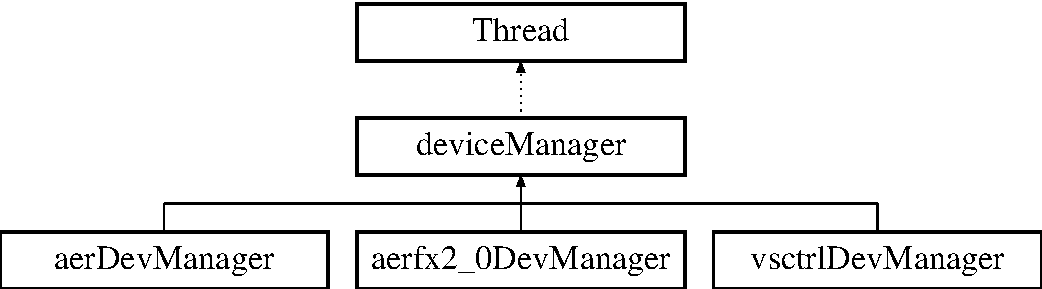
\includegraphics[height=3.000000cm]{classdeviceManager}
\end{center}
\end{figure}
\subsection*{Public Member Functions}
\begin{DoxyCompactItemize}
\item 
\hypertarget{classdeviceManager_ad3fd308a8add5e51c1c145896bc2daf9}{virtual bool {\bfseries open\-Device} ()}\label{classdeviceManager_ad3fd308a8add5e51c1c145896bc2daf9}

\item 
\hypertarget{classdeviceManager_ae643291e5d1732bfe72032ea62c5253b}{virtual void {\bfseries close\-Device} ()}\label{classdeviceManager_ae643291e5d1732bfe72032ea62c5253b}

\item 
\hypertarget{classdeviceManager_a368b612f7207d4777351fbb58ae92682}{int {\bfseries write\-Device} (std\-::vector$<$ unsigned int $>$ \&device\-Data)}\label{classdeviceManager_a368b612f7207d4777351fbb58ae92682}

\item 
\hypertarget{classdeviceManager_abb8987142dce5d83c05773576a643f50}{const std\-::vector$<$ char $>$ \& {\bfseries read\-Device} (int \&n\-Bytes\-Read)}\label{classdeviceManager_abb8987142dce5d83c05773576a643f50}

\item 
\hypertarget{classdeviceManager_a1cbcde6f497b8472b873e739f75e92e4}{{\bfseries device\-Manager} (bool buffered\-Read=false, unsigned int max\-Buffer\-Size=M\-A\-X\-\_\-\-B\-U\-F\-\_\-\-S\-I\-Z\-E)}\label{classdeviceManager_a1cbcde6f497b8472b873e739f75e92e4}

\item 
\hypertarget{classdeviceManager_a16183255591219aaf6986997a486ff6a}{const unsigned int {\bfseries get\-Buffer\-Size} ()}\label{classdeviceManager_a16183255591219aaf6986997a486ff6a}

\item 
\hypertarget{classdeviceManager_a5e0e8c642ce32a7e7a435a8cbc563576}{const std\-::string {\bfseries get\-Dev\-Type} ()}\label{classdeviceManager_a5e0e8c642ce32a7e7a435a8cbc563576}

\end{DoxyCompactItemize}
\subsection*{Protected Attributes}
\begin{DoxyCompactItemize}
\item 
\hypertarget{classdeviceManager_af9556035e202ee95a17f2ecf5b7101db}{bool {\bfseries buffered\-Read}}\label{classdeviceManager_af9556035e202ee95a17f2ecf5b7101db}

\item 
\hypertarget{classdeviceManager_a1918c9e6863e6465e5d34ca86edcbfb7}{int {\bfseries dev\-Desc}}\label{classdeviceManager_a1918c9e6863e6465e5d34ca86edcbfb7}

\item 
\hypertarget{classdeviceManager_a6065df91f833483f38887ca5c1fea141}{std\-::string {\bfseries device\-Name}}\label{classdeviceManager_a6065df91f833483f38887ca5c1fea141}

\end{DoxyCompactItemize}


\subsection{Detailed Description}
The \hyperlink{classdeviceManager}{device\-Manager} class opens the device and implements a constant read. 

The documentation for this class was generated from the following files\-:\begin{DoxyCompactItemize}
\item 
/home/aglover/workspace/projects/event\-Driven/src/grabbers/zynq\-Grabber/include/i\-Cub/device\-Manager.\-h\item 
/home/aglover/workspace/projects/event\-Driven/src/grabbers/zynq\-Grabber/src/device\-Manager.\-cpp\end{DoxyCompactItemize}

\hypertarget{classdPepperIO}{\section{d\-Pepper\-I\-O Class Reference}
\label{classdPepperIO}\index{d\-Pepper\-I\-O@{d\-Pepper\-I\-O}}
}
Inheritance diagram for d\-Pepper\-I\-O\-:\begin{figure}[H]
\begin{center}
\leavevmode
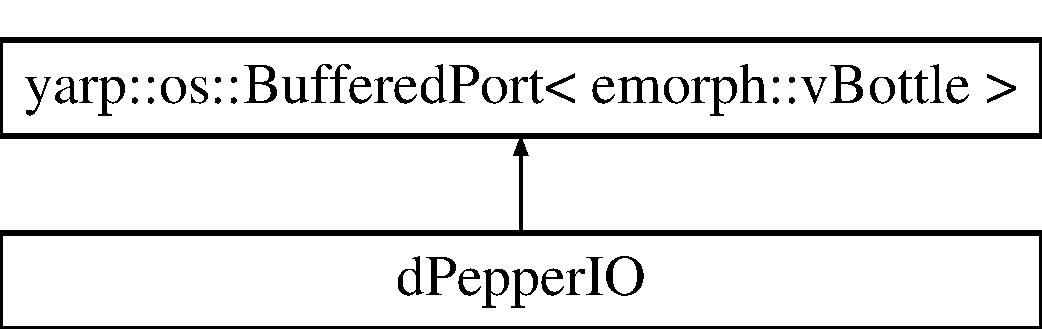
\includegraphics[height=2.000000cm]{classdPepperIO}
\end{center}
\end{figure}
\subsection*{Public Member Functions}
\begin{DoxyCompactItemize}
\item 
\hypertarget{classdPepperIO_ae015f55221ff1e2f670f50cc31289051}{bool {\bfseries open} (const std\-::string \&name)}\label{classdPepperIO_ae015f55221ff1e2f670f50cc31289051}

\item 
\hypertarget{classdPepperIO_a1df29cd021e0c84fa7740384ed2eaa28}{void {\bfseries close} ()}\label{classdPepperIO_a1df29cd021e0c84fa7740384ed2eaa28}

\item 
\hypertarget{classdPepperIO_a592854be686238b0389ebd95c994f118}{void {\bfseries interrupt} ()}\label{classdPepperIO_a592854be686238b0389ebd95c994f118}

\item 
\hypertarget{classdPepperIO_a5a6c8c66d20df7a8c95084eec8e02a11}{void {\bfseries on\-Read} (\hyperlink{classemorph_1_1vBottle}{emorph\-::v\-Bottle} \&bot)}\label{classdPepperIO_a5a6c8c66d20df7a8c95084eec8e02a11}

\item 
\hypertarget{classdPepperIO_a9318fc518ca2798fed718f134cbcb263}{void {\bfseries set\-Temporal\-Size} (double microseconds)}\label{classdPepperIO_a9318fc518ca2798fed718f134cbcb263}

\item 
\hypertarget{classdPepperIO_abcd23de652bc8eeb1e6c577b71304a16}{void {\bfseries set\-Spatial\-Size} (double pixelradius)}\label{classdPepperIO_abcd23de652bc8eeb1e6c577b71304a16}

\end{DoxyCompactItemize}


The documentation for this class was generated from the following files\-:\begin{DoxyCompactItemize}
\item 
/home/aglover/workspace/projects/event\-Driven/src/processing/v\-Pepper/include/d\-Pepper.\-h\item 
/home/aglover/workspace/projects/event\-Driven/src/processing/v\-Pepper/src/d\-Pepper.\-cpp\end{DoxyCompactItemize}

\hypertarget{classdPepperModule}{\section{d\-Pepper\-Module Class Reference}
\label{classdPepperModule}\index{d\-Pepper\-Module@{d\-Pepper\-Module}}
}
Inheritance diagram for d\-Pepper\-Module\-:\begin{figure}[H]
\begin{center}
\leavevmode
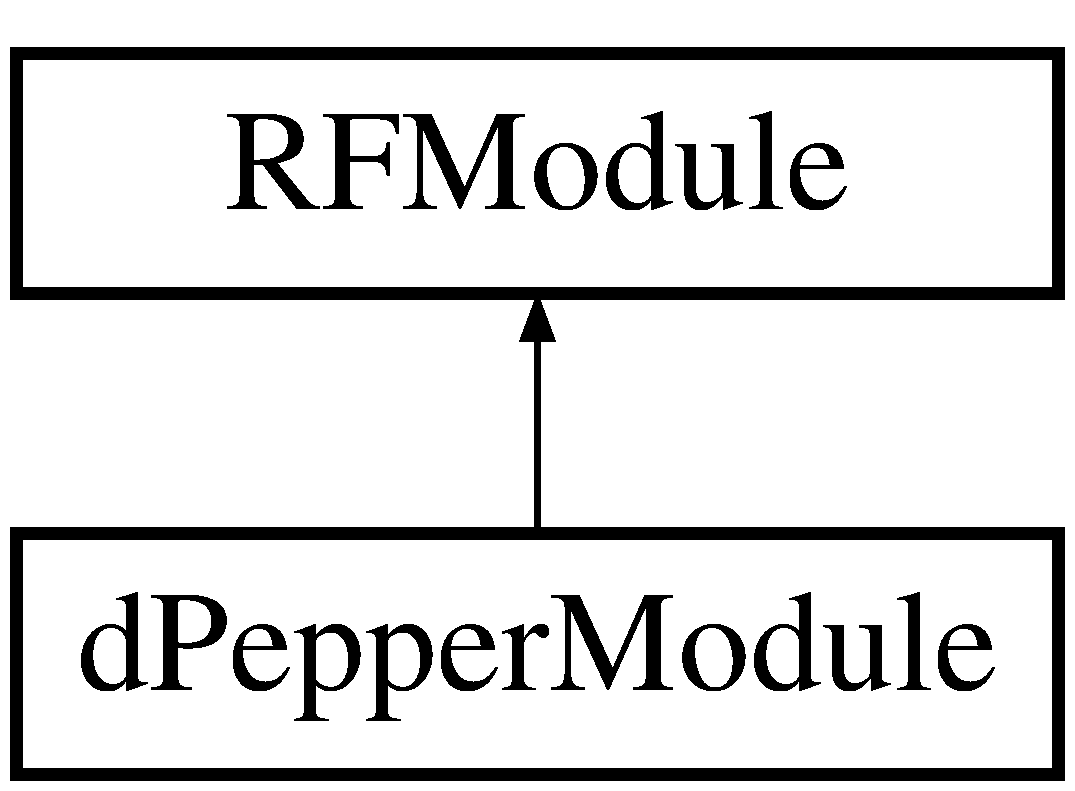
\includegraphics[height=2.000000cm]{classdPepperModule}
\end{center}
\end{figure}
\subsection*{Public Member Functions}
\begin{DoxyCompactItemize}
\item 
\hypertarget{classdPepperModule_a11343b0bb91bfbc6e4f0f7252ec735e0}{virtual bool {\bfseries configure} (yarp\-::os\-::\-Resource\-Finder \&rf)}\label{classdPepperModule_a11343b0bb91bfbc6e4f0f7252ec735e0}

\item 
\hypertarget{classdPepperModule_a7db49020f01515fbf8b3b8e43637f5d0}{virtual bool {\bfseries interrupt\-Module} ()}\label{classdPepperModule_a7db49020f01515fbf8b3b8e43637f5d0}

\item 
\hypertarget{classdPepperModule_a0f53fec8e6d6c2b6619d874bf21d25a9}{virtual bool {\bfseries close} ()}\label{classdPepperModule_a0f53fec8e6d6c2b6619d874bf21d25a9}

\item 
\hypertarget{classdPepperModule_a893991e035a6f52815d3fa73425a5532}{virtual double {\bfseries get\-Period} ()}\label{classdPepperModule_a893991e035a6f52815d3fa73425a5532}

\item 
\hypertarget{classdPepperModule_accac55827cea616f7d27102491f58f8e}{virtual bool {\bfseries update\-Module} ()}\label{classdPepperModule_accac55827cea616f7d27102491f58f8e}

\end{DoxyCompactItemize}


The documentation for this class was generated from the following files\-:\begin{DoxyCompactItemize}
\item 
/home/aglover/workspace/projects/event\-Driven/src/processing/v\-Pepper/include/d\-Pepper.\-h\item 
/home/aglover/workspace/projects/event\-Driven/src/processing/v\-Pepper/src/d\-Pepper.\-cpp\end{DoxyCompactItemize}

\hypertarget{classeventBottle}{\section{event\-Bottle Class Reference}
\label{classeventBottle}\index{event\-Bottle@{event\-Bottle}}
}


{\ttfamily \#include $<$event\-Bottle.\-h$>$}

Inheritance diagram for event\-Bottle\-:\begin{figure}[H]
\begin{center}
\leavevmode
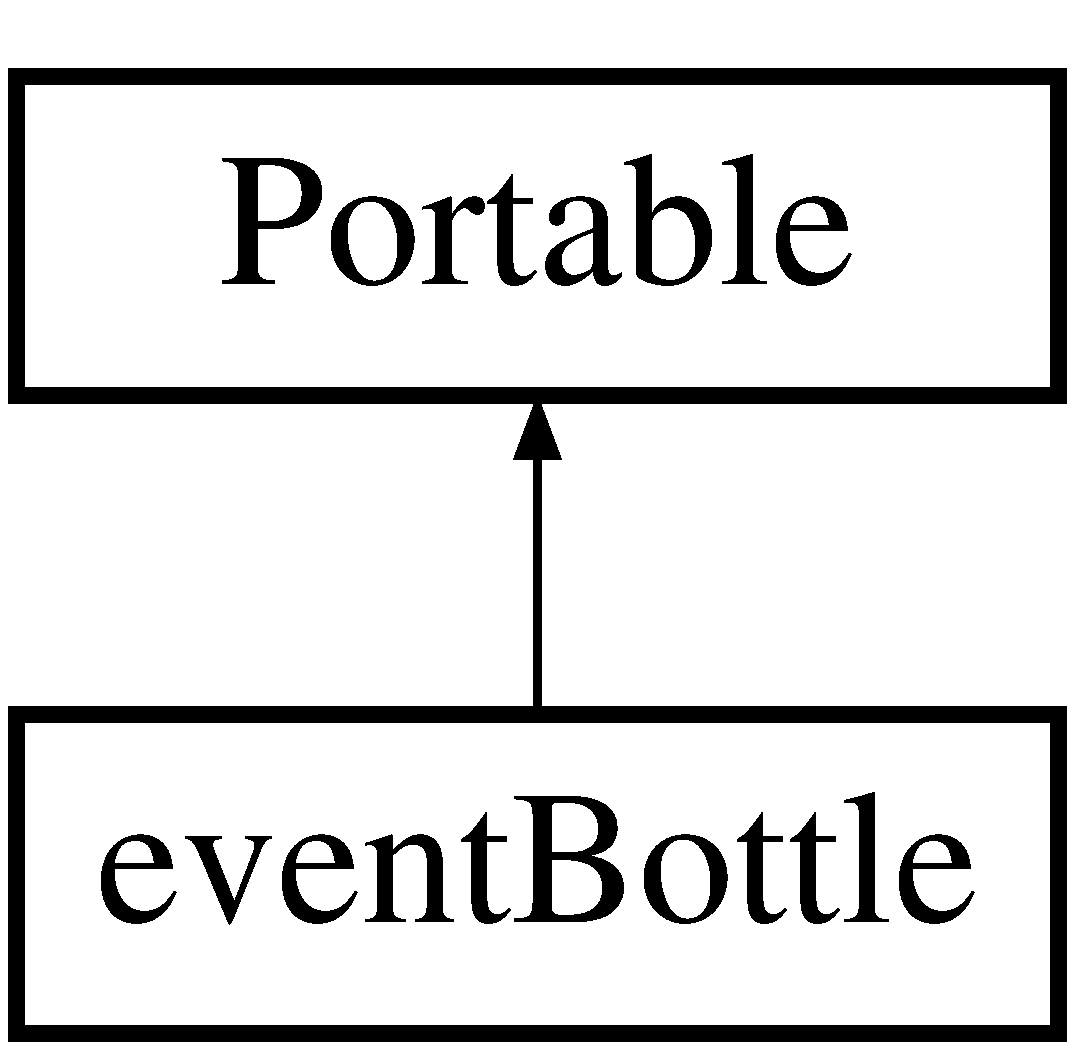
\includegraphics[height=2.000000cm]{classeventBottle}
\end{center}
\end{figure}
\subsection*{Public Member Functions}
\begin{DoxyCompactItemize}
\item 
\hyperlink{classeventBottle_aa1fbb7e85119920debfccc223f2843f1}{event\-Bottle} ()
\item 
\hyperlink{classeventBottle_a44740910c0137e62aa3b4c3860109497}{event\-Bottle} (char $\ast$c, int i)
\begin{DoxyCompactList}\small\item\em constructor \end{DoxyCompactList}\item 
\hyperlink{classeventBottle_a29410be24e171cf5d73ee073712b062e}{event\-Bottle} (yarp\-::os\-::\-Bottle $\ast$b)
\begin{DoxyCompactList}\small\item\em constructor \end{DoxyCompactList}\item 
\hyperlink{classeventBottle_a2c1c9f1259b33b74f8e0b9111df47a39}{$\sim$event\-Bottle} ()
\item 
\hypertarget{classeventBottle_aa238f06090b0fb1e25592f8a188401d9}{void {\bfseries operator=} (\hyperlink{classeventBottle}{event\-Bottle} \&)}\label{classeventBottle_aa238f06090b0fb1e25592f8a188401d9}

\item 
\hypertarget{classeventBottle_a7cf605ab90defeb9da312a91eb55ac46}{\hyperlink{classeventBottle_a7cf605ab90defeb9da312a91eb55ac46}{event\-Bottle} (const \hyperlink{classeventBottle}{event\-Bottle} \&)}\label{classeventBottle_a7cf605ab90defeb9da312a91eb55ac46}

\begin{DoxyCompactList}\small\item\em copy constructor \end{DoxyCompactList}\item 
\hypertarget{classeventBottle_a524fd9080ab98e87f89e548c83c695fa}{virtual bool {\bfseries write} (yarp\-::os\-::\-Connection\-Writer \&)}\label{classeventBottle_a524fd9080ab98e87f89e548c83c695fa}

\item 
\hypertarget{classeventBottle_a2601d1ced98aea595bec4917c680fe71}{virtual bool {\bfseries read} (yarp\-::os\-::\-Connection\-Reader \&)}\label{classeventBottle_a2601d1ced98aea595bec4917c680fe71}

\item 
void \hyperlink{classeventBottle_a75ea08df0fd8ce6cf8331678ef587413}{set\-\_\-data} (char $\ast$c, int i)
\begin{DoxyCompactList}\small\item\em function for setting the data afterward \end{DoxyCompactList}\item 
void \hyperlink{classeventBottle_ade587dd59d1a5f1a84de281b9aa119f5}{set\-\_\-data} (yarp\-::os\-::\-Bottle $\ast$b)
\begin{DoxyCompactList}\small\item\em function for setting the data afterward \end{DoxyCompactList}\item 
\hypertarget{classeventBottle_a59afc1ae08a0392ecd34fddff82319da}{yarp\-::os\-::\-Bottle $\ast$ {\bfseries get\-\_\-packet} ()}\label{classeventBottle_a59afc1ae08a0392ecd34fddff82319da}

\item 
\hypertarget{classeventBottle_a81a5715c8f7f59af32e792c77695dbac}{int {\bfseries get\-\_\-size\-Of\-Packet} ()}\label{classeventBottle_a81a5715c8f7f59af32e792c77695dbac}

\item 
\hypertarget{classeventBottle_ac0a84996be2cf4da895423d1b4d4632d}{int {\bfseries get\-\_\-bytes\-Of\-Packet} ()}\label{classeventBottle_ac0a84996be2cf4da895423d1b4d4632d}

\item 
\hypertarget{classeventBottle_ad80009e5ff12f9fc2611818ea3c12d42}{int {\bfseries get\-\_\-size\-Of\-Bottle} ()}\label{classeventBottle_ad80009e5ff12f9fc2611818ea3c12d42}

\end{DoxyCompactItemize}


\subsection{Detailed Description}
portable class for the bottle of events 

\subsection{Constructor \& Destructor Documentation}
\hypertarget{classeventBottle_aa1fbb7e85119920debfccc223f2843f1}{\index{event\-Bottle@{event\-Bottle}!event\-Bottle@{event\-Bottle}}
\index{event\-Bottle@{event\-Bottle}!eventBottle@{event\-Bottle}}
\subsubsection[{event\-Bottle}]{\setlength{\rightskip}{0pt plus 5cm}event\-Bottle\-::event\-Bottle (
\begin{DoxyParamCaption}
{}
\end{DoxyParamCaption}
)}}\label{classeventBottle_aa1fbb7e85119920debfccc223f2843f1}
default constructor \hypertarget{classeventBottle_a44740910c0137e62aa3b4c3860109497}{\index{event\-Bottle@{event\-Bottle}!event\-Bottle@{event\-Bottle}}
\index{event\-Bottle@{event\-Bottle}!eventBottle@{event\-Bottle}}
\subsubsection[{event\-Bottle}]{\setlength{\rightskip}{0pt plus 5cm}event\-Bottle\-::event\-Bottle (
\begin{DoxyParamCaption}
\item[{char $\ast$}]{c, }
\item[{int}]{i}
\end{DoxyParamCaption}
)}}\label{classeventBottle_a44740910c0137e62aa3b4c3860109497}


constructor 


\begin{DoxyParams}{Parameters}
{\em c} & pointer to the char buffer \\
\hline
{\em i} & number of bytes \\
\hline
\end{DoxyParams}
\hypertarget{classeventBottle_a29410be24e171cf5d73ee073712b062e}{\index{event\-Bottle@{event\-Bottle}!event\-Bottle@{event\-Bottle}}
\index{event\-Bottle@{event\-Bottle}!eventBottle@{event\-Bottle}}
\subsubsection[{event\-Bottle}]{\setlength{\rightskip}{0pt plus 5cm}event\-Bottle\-::event\-Bottle (
\begin{DoxyParamCaption}
\item[{yarp\-::os\-::\-Bottle $\ast$}]{b}
\end{DoxyParamCaption}
)}}\label{classeventBottle_a29410be24e171cf5d73ee073712b062e}


constructor 


\begin{DoxyParams}{Parameters}
{\em b} & bottle that constructs the class\\
\hline
\end{DoxyParams}
constructor from a bottle \hypertarget{classeventBottle_a2c1c9f1259b33b74f8e0b9111df47a39}{\index{event\-Bottle@{event\-Bottle}!$\sim$event\-Bottle@{$\sim$event\-Bottle}}
\index{$\sim$event\-Bottle@{$\sim$event\-Bottle}!eventBottle@{event\-Bottle}}
\subsubsection[{$\sim$event\-Bottle}]{\setlength{\rightskip}{0pt plus 5cm}event\-Bottle\-::$\sim$event\-Bottle (
\begin{DoxyParamCaption}
{}
\end{DoxyParamCaption}
)}}\label{classeventBottle_a2c1c9f1259b33b74f8e0b9111df47a39}
destructor 

\subsection{Member Function Documentation}
\hypertarget{classeventBottle_a75ea08df0fd8ce6cf8331678ef587413}{\index{event\-Bottle@{event\-Bottle}!set\-\_\-data@{set\-\_\-data}}
\index{set\-\_\-data@{set\-\_\-data}!eventBottle@{event\-Bottle}}
\subsubsection[{set\-\_\-data}]{\setlength{\rightskip}{0pt plus 5cm}void event\-Bottle\-::set\-\_\-data (
\begin{DoxyParamCaption}
\item[{char $\ast$}]{c, }
\item[{int}]{i}
\end{DoxyParamCaption}
)}}\label{classeventBottle_a75ea08df0fd8ce6cf8331678ef587413}


function for setting the data afterward 


\begin{DoxyParams}{Parameters}
{\em c} & pointer to the char buffer of events \\
\hline
{\em i} & number of bytes in the buffer \\
\hline
\end{DoxyParams}
\hypertarget{classeventBottle_ade587dd59d1a5f1a84de281b9aa119f5}{\index{event\-Bottle@{event\-Bottle}!set\-\_\-data@{set\-\_\-data}}
\index{set\-\_\-data@{set\-\_\-data}!eventBottle@{event\-Bottle}}
\subsubsection[{set\-\_\-data}]{\setlength{\rightskip}{0pt plus 5cm}void event\-Bottle\-::set\-\_\-data (
\begin{DoxyParamCaption}
\item[{yarp\-::os\-::\-Bottle $\ast$}]{b}
\end{DoxyParamCaption}
)}}\label{classeventBottle_ade587dd59d1a5f1a84de281b9aa119f5}


function for setting the data afterward 


\begin{DoxyParams}{Parameters}
{\em b} & bottle pointer \\
\hline
\end{DoxyParams}


The documentation for this class was generated from the following files\-:\begin{DoxyCompactItemize}
\item 
/home/aglover/workspace/projects/event\-Driven/emorph\-\_\-lib/include/i\-Cub/emorph/event\-Bottle.\-h\item 
/home/aglover/workspace/projects/event\-Driven/emorph\-\_\-lib/src/event\-Bottle.\-cpp\end{DoxyCompactItemize}

\hypertarget{classEventBottleManager}{\section{Event\-Bottle\-Manager Class Reference}
\label{classEventBottleManager}\index{Event\-Bottle\-Manager@{Event\-Bottle\-Manager}}
}
Inheritance diagram for Event\-Bottle\-Manager\-:\begin{figure}[H]
\begin{center}
\leavevmode
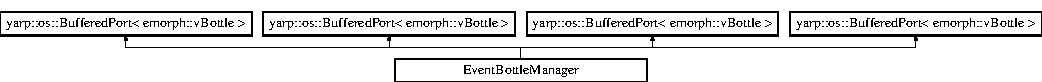
\includegraphics[height=1.106719cm]{classEventBottleManager}
\end{center}
\end{figure}
\subsection*{Public Member Functions}
\begin{DoxyCompactItemize}
\item 
\hypertarget{classEventBottleManager_a41ce7bd0a716ab0a88c1ad505b02d20b}{bool {\bfseries open} (const std\-::string \&name)}\label{classEventBottleManager_a41ce7bd0a716ab0a88c1ad505b02d20b}

\item 
\hypertarget{classEventBottleManager_a9571d64d4640ef5a38f03a286d27425e}{void {\bfseries on\-Read} (\hyperlink{classemorph_1_1vBottle}{emorph\-::v\-Bottle} \&bot)}\label{classEventBottleManager_a9571d64d4640ef5a38f03a286d27425e}

\item 
\hypertarget{classEventBottleManager_af15b5cfdc457500423111c22dee264d2}{unsigned long int {\bfseries get\-Time} ()}\label{classEventBottleManager_af15b5cfdc457500423111c22dee264d2}

\item 
\hypertarget{classEventBottleManager_a0b4fd036f14e713194d079467021ba3b}{unsigned long int {\bfseries pop\-Count} ()}\label{classEventBottleManager_a0b4fd036f14e713194d079467021ba3b}

\item 
\hypertarget{classEventBottleManager_a41ce7bd0a716ab0a88c1ad505b02d20b}{bool {\bfseries open} (const std\-::string \&name)}\label{classEventBottleManager_a41ce7bd0a716ab0a88c1ad505b02d20b}

\item 
\hypertarget{classEventBottleManager_aa155dc6f20728e9f7ff13abf720ea6b8}{void {\bfseries close} ()}\label{classEventBottleManager_aa155dc6f20728e9f7ff13abf720ea6b8}

\item 
\hypertarget{classEventBottleManager_a15152f9daa40714334c2da3871f959a9}{void {\bfseries interrupt} ()}\label{classEventBottleManager_a15152f9daa40714334c2da3871f959a9}

\item 
\hypertarget{classEventBottleManager_a9571d64d4640ef5a38f03a286d27425e}{void {\bfseries on\-Read} (\hyperlink{classemorph_1_1vBottle}{emorph\-::v\-Bottle} \&bot)}\label{classEventBottleManager_a9571d64d4640ef5a38f03a286d27425e}

\item 
\hypertarget{classEventBottleManager_a451485cebdadbbad730d176894d9f0b1}{void {\bfseries set\-All\-Parameters} (double alpha\-\_\-shape, double alpha\-\_\-pos, double Tact, double Tinact, double Tfree, double Tevent, double Sig\-X, double Sig\-Y, double Sig\-X\-Y, bool Fixedshape, int Regrate, double Maxdist, double decay\-\_\-tau, double cluster\-Limit)}\label{classEventBottleManager_a451485cebdadbbad730d176894d9f0b1}

\item 
\hypertarget{classEventBottleManager_a82d3237530dcc455f3ceae4e1db4f6df}{bool {\bfseries open} (std\-::string module\-Name)}\label{classEventBottleManager_a82d3237530dcc455f3ceae4e1db4f6df}

\item 
\hypertarget{classEventBottleManager_af4d71177a30fdd8fc40485b91abdae10}{bool {\bfseries init} ()}\label{classEventBottleManager_af4d71177a30fdd8fc40485b91abdae10}

\item 
\hypertarget{classEventBottleManager_aa155dc6f20728e9f7ff13abf720ea6b8}{void {\bfseries close} ()}\label{classEventBottleManager_aa155dc6f20728e9f7ff13abf720ea6b8}

\item 
\hypertarget{classEventBottleManager_a9571d64d4640ef5a38f03a286d27425e}{void {\bfseries on\-Read} (\hyperlink{classemorph_1_1vBottle}{emorph\-::v\-Bottle} \&bot)}\label{classEventBottleManager_a9571d64d4640ef5a38f03a286d27425e}

\item 
\hypertarget{classEventBottleManager_a15152f9daa40714334c2da3871f959a9}{void {\bfseries interrupt} ()}\label{classEventBottleManager_a15152f9daa40714334c2da3871f959a9}

\item 
\hypertarget{classEventBottleManager_a756fda9127e0fc1f8b3781f905f6d28a}{void {\bfseries set\-Sensor\-Size} (int sensor\-Height, int sensor\-Width)}\label{classEventBottleManager_a756fda9127e0fc1f8b3781f905f6d28a}

\item 
\hypertarget{classEventBottleManager_abf9943ffed44f78430eb1f49e469beb5}{bool {\bfseries set\-To\-Truncate} (bool truncate)}\label{classEventBottleManager_abf9943ffed44f78430eb1f49e469beb5}

\item 
\hypertarget{classEventBottleManager_ab22a4a1446b8eb35a377fcd7552c63ea}{bool {\bfseries set\-Cam\-Params} (const yarp\-::os\-::\-Bottle \&left, const yarp\-::os\-::\-Bottle \&right)}\label{classEventBottleManager_ab22a4a1446b8eb35a377fcd7552c63ea}

\item 
\hypertarget{classEventBottleManager_a41ce7bd0a716ab0a88c1ad505b02d20b}{bool {\bfseries open} (const std\-::string \&name)}\label{classEventBottleManager_a41ce7bd0a716ab0a88c1ad505b02d20b}

\item 
\hypertarget{classEventBottleManager_aa155dc6f20728e9f7ff13abf720ea6b8}{void {\bfseries close} ()}\label{classEventBottleManager_aa155dc6f20728e9f7ff13abf720ea6b8}

\item 
\hypertarget{classEventBottleManager_a15152f9daa40714334c2da3871f959a9}{void {\bfseries interrupt} ()}\label{classEventBottleManager_a15152f9daa40714334c2da3871f959a9}

\item 
\hypertarget{classEventBottleManager_a9571d64d4640ef5a38f03a286d27425e}{void {\bfseries on\-Read} (\hyperlink{classemorph_1_1vBottle}{emorph\-::v\-Bottle} \&bot)}\label{classEventBottleManager_a9571d64d4640ef5a38f03a286d27425e}

\end{DoxyCompactItemize}


The documentation for this class was generated from the following files\-:\begin{DoxyCompactItemize}
\item 
/home/aglover/workspace/projects/event\-Driven/src/movement/autosaccade/include/auto\-Saccade.\-h\item 
/home/aglover/workspace/projects/event\-Driven/src/processing/template/include/v\-Template.\-h\item 
/home/aglover/workspace/projects/event\-Driven/src/processing/v\-Cluster/include/event\-Clustering.\-h\item 
/home/aglover/workspace/projects/event\-Driven/src/processing/v\-Undistort\-Cam/include/v\-Undistort\-Cam.\-h\item 
/home/aglover/workspace/projects/event\-Driven/src/movement/autosaccade/src/auto\-Saccade.\-cpp\item 
/home/aglover/workspace/projects/event\-Driven/src/processing/template/src/v\-Template.\-cpp\item 
/home/aglover/workspace/projects/event\-Driven/src/processing/v\-Cluster/src/event\-Clustering.\-cpp\item 
/home/aglover/workspace/projects/event\-Driven/src/processing/v\-Undistort\-Cam/src/v\-Undistort\-Cam.\-cpp\end{DoxyCompactItemize}

\hypertarget{classemorph_1_1ebuffer_1_1eventBuffer}{\section{emorph\-:\-:ebuffer\-:\-:event\-Buffer Class Reference}
\label{classemorph_1_1ebuffer_1_1eventBuffer}\index{emorph\-::ebuffer\-::event\-Buffer@{emorph\-::ebuffer\-::event\-Buffer}}
}
Inheritance diagram for emorph\-:\-:ebuffer\-:\-:event\-Buffer\-:\begin{figure}[H]
\begin{center}
\leavevmode
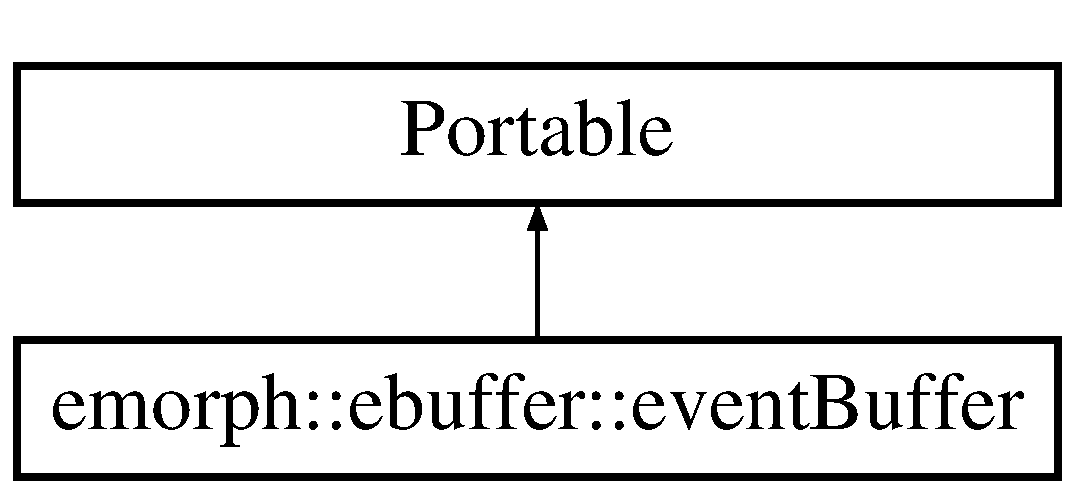
\includegraphics[height=2.000000cm]{classemorph_1_1ebuffer_1_1eventBuffer}
\end{center}
\end{figure}
\subsection*{Public Member Functions}
\begin{DoxyCompactItemize}
\item 
\hypertarget{classemorph_1_1ebuffer_1_1eventBuffer_a9e13c98fa7c63efec7258906e904ed16}{{\bfseries event\-Buffer} (char $\ast$, int)}\label{classemorph_1_1ebuffer_1_1eventBuffer_a9e13c98fa7c63efec7258906e904ed16}

\item 
\hypertarget{classemorph_1_1ebuffer_1_1eventBuffer_a00dfcb30ed67ac86ac014c9902fcf317}{void {\bfseries operator=} (const \hyperlink{classemorph_1_1ebuffer_1_1eventBuffer}{event\-Buffer} \&)}\label{classemorph_1_1ebuffer_1_1eventBuffer_a00dfcb30ed67ac86ac014c9902fcf317}

\item 
\hypertarget{classemorph_1_1ebuffer_1_1eventBuffer_abd14b10547d4ed68cad1c401c8f36299}{{\bfseries event\-Buffer} (const \hyperlink{classemorph_1_1ebuffer_1_1eventBuffer}{event\-Buffer} \&)}\label{classemorph_1_1ebuffer_1_1eventBuffer_abd14b10547d4ed68cad1c401c8f36299}

\item 
\hypertarget{classemorph_1_1ebuffer_1_1eventBuffer_ab57bd7441586fc6cf97e0a8e281939ce}{virtual bool {\bfseries write} (yarp\-::os\-::\-Connection\-Writer \&)}\label{classemorph_1_1ebuffer_1_1eventBuffer_ab57bd7441586fc6cf97e0a8e281939ce}

\item 
\hypertarget{classemorph_1_1ebuffer_1_1eventBuffer_aed15424c857c10d248f968dab733e810}{virtual bool {\bfseries read} (yarp\-::os\-::\-Connection\-Reader \&)}\label{classemorph_1_1ebuffer_1_1eventBuffer_aed15424c857c10d248f968dab733e810}

\item 
\hypertarget{classemorph_1_1ebuffer_1_1eventBuffer_ac08b4f00bdf56c1ffc223a19d97ab868}{void {\bfseries set\-\_\-data} (char $\ast$, int)}\label{classemorph_1_1ebuffer_1_1eventBuffer_ac08b4f00bdf56c1ffc223a19d97ab868}

\item 
\hypertarget{classemorph_1_1ebuffer_1_1eventBuffer_a882d4c01a10332da6ccfede46f875057}{char $\ast$ {\bfseries get\-\_\-packet} ()}\label{classemorph_1_1ebuffer_1_1eventBuffer_a882d4c01a10332da6ccfede46f875057}

\item 
\hypertarget{classemorph_1_1ebuffer_1_1eventBuffer_a7fe698e32c183bc5787369728cc59469}{int {\bfseries get\-\_\-size\-Of\-Packet} ()}\label{classemorph_1_1ebuffer_1_1eventBuffer_a7fe698e32c183bc5787369728cc59469}

\end{DoxyCompactItemize}


The documentation for this class was generated from the following files\-:\begin{DoxyCompactItemize}
\item 
/home/aglover/workspace/projects/event\-Driven/emorph\-\_\-lib/include/i\-Cub/emorph/event\-Buffer.\-h\item 
/home/aglover/workspace/projects/event\-Driven/emorph\-\_\-lib/src/event\-Buffer.\-cpp\end{DoxyCompactItemize}

\hypertarget{classEventClustering}{\section{Event\-Clustering Class Reference}
\label{classEventClustering}\index{Event\-Clustering@{Event\-Clustering}}
}
Inheritance diagram for Event\-Clustering\-:\begin{figure}[H]
\begin{center}
\leavevmode
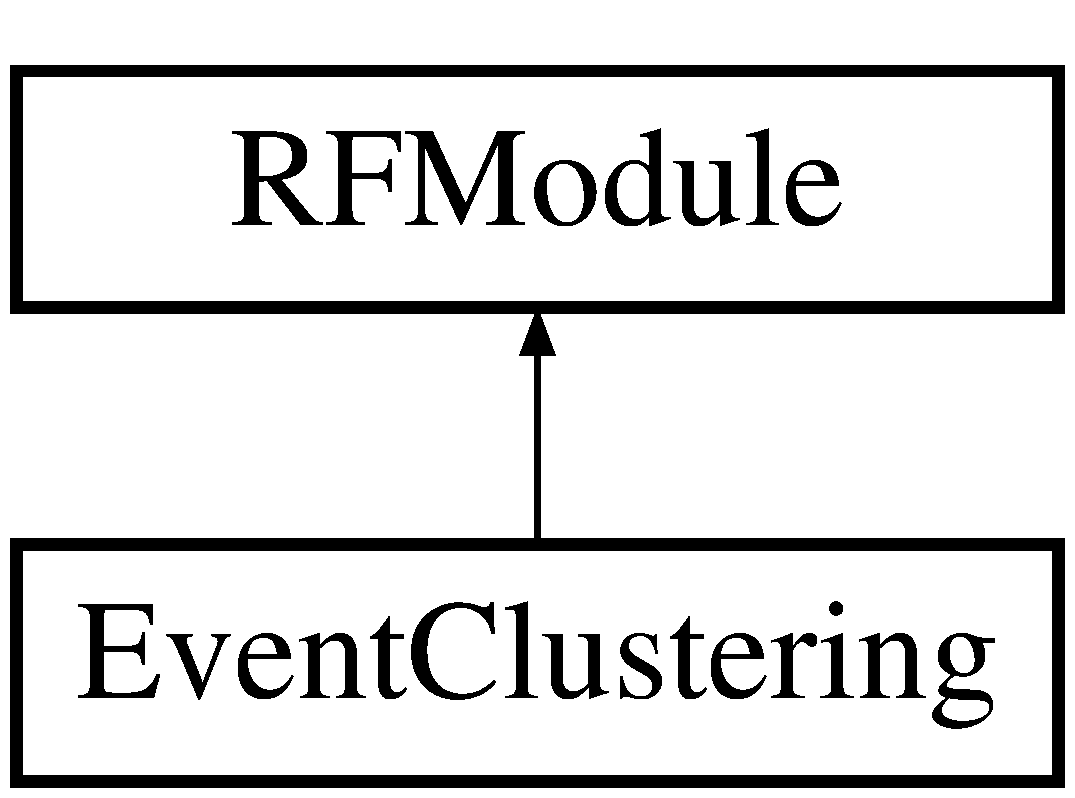
\includegraphics[height=2.000000cm]{classEventClustering}
\end{center}
\end{figure}
\subsection*{Public Member Functions}
\begin{DoxyCompactItemize}
\item 
\hypertarget{classEventClustering_a9111f5db3d21a2a80bef0ac5a6996d06}{bool {\bfseries configure} (yarp\-::os\-::\-Resource\-Finder \&rf)}\label{classEventClustering_a9111f5db3d21a2a80bef0ac5a6996d06}

\item 
\hypertarget{classEventClustering_adb2bb1f480ac61629327d5170dd64398}{bool {\bfseries interrupt\-Module} ()}\label{classEventClustering_adb2bb1f480ac61629327d5170dd64398}

\item 
\hypertarget{classEventClustering_af27e70c40cdfddab01c1fffed35620a3}{bool {\bfseries close} ()}\label{classEventClustering_af27e70c40cdfddab01c1fffed35620a3}

\item 
\hypertarget{classEventClustering_afe356ead5fe50d67b2007e3f99f7818f}{double {\bfseries get\-Period} ()}\label{classEventClustering_afe356ead5fe50d67b2007e3f99f7818f}

\item 
\hypertarget{classEventClustering_a25159637f1dc8c9cd27cde191b7296d2}{bool {\bfseries update\-Module} ()}\label{classEventClustering_a25159637f1dc8c9cd27cde191b7296d2}

\end{DoxyCompactItemize}


The documentation for this class was generated from the following files\-:\begin{DoxyCompactItemize}
\item 
/home/aglover/workspace/projects/event\-Driven/src/processing/v\-Cluster/include/event\-Clustering.\-h\item 
/home/aglover/workspace/projects/event\-Driven/src/processing/v\-Cluster/src/event\-Clustering.\-cpp\end{DoxyCompactItemize}

\hypertarget{classemorph_1_1eventProcessor}{\section{emorph\-:\-:event\-Processor Class Reference}
\label{classemorph_1_1eventProcessor}\index{emorph\-::event\-Processor@{emorph\-::event\-Processor}}
}
\subsection*{Public Member Functions}
\begin{DoxyCompactItemize}
\item 
\hypertarget{classemorph_1_1eventProcessor_a333c21041a0998eb2739900a0eb75752}{\hyperlink{classemorph_1_1vEvent}{emorph\-::v\-Event} \& {\bfseries my\-Func} (\hyperlink{classemorph_1_1vEvent}{emorph\-::v\-Event} \&event)}\label{classemorph_1_1eventProcessor_a333c21041a0998eb2739900a0eb75752}

\end{DoxyCompactItemize}


The documentation for this class was generated from the following files\-:\begin{DoxyCompactItemize}
\item 
/home/aglover/workspace/projects/event\-Driven/src/processing/template/include/v\-Template\-Process.\-h\item 
/home/aglover/workspace/projects/event\-Driven/src/processing/template/src/v\-Template\-Process.\-cpp\end{DoxyCompactItemize}

\hypertarget{classeventStatisticsDumper}{\section{event\-Statistics\-Dumper Class Reference}
\label{classeventStatisticsDumper}\index{event\-Statistics\-Dumper@{event\-Statistics\-Dumper}}
}
Inheritance diagram for event\-Statistics\-Dumper\-:\begin{figure}[H]
\begin{center}
\leavevmode
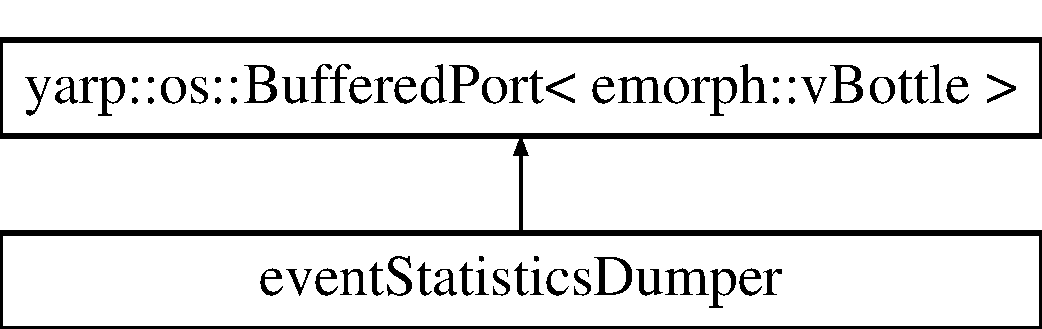
\includegraphics[height=2.000000cm]{classeventStatisticsDumper}
\end{center}
\end{figure}
\subsection*{Public Member Functions}
\begin{DoxyCompactItemize}
\item 
\hypertarget{classeventStatisticsDumper_ae19ee350a1d131d0c54e0f7ac2437397}{bool {\bfseries open} (std\-::string module\-Name=\char`\"{}E\-S\-D\char`\"{})}\label{classeventStatisticsDumper_ae19ee350a1d131d0c54e0f7ac2437397}

\item 
\hypertarget{classeventStatisticsDumper_a5373c7abee32f595308f59c3d2c02c01}{void {\bfseries on\-Read} (\hyperlink{classemorph_1_1vBottle}{emorph\-::v\-Bottle} \&bot)}\label{classeventStatisticsDumper_a5373c7abee32f595308f59c3d2c02c01}

\item 
\hypertarget{classeventStatisticsDumper_aea5b77b83db3a9955e8fd8322d91dea1}{void {\bfseries close} ()}\label{classeventStatisticsDumper_aea5b77b83db3a9955e8fd8322d91dea1}

\item 
\hypertarget{classeventStatisticsDumper_a48c32b38d277f6b735c78cfbad6bcb64}{void {\bfseries set\-Directory} (std\-::string dir)}\label{classeventStatisticsDumper_a48c32b38d277f6b735c78cfbad6bcb64}

\item 
\hypertarget{classeventStatisticsDumper_af593efeee949a19d018aea33cbc5281a}{int {\bfseries get\-Bottle\-Count} ()}\label{classeventStatisticsDumper_af593efeee949a19d018aea33cbc5281a}

\end{DoxyCompactItemize}


The documentation for this class was generated from the following files\-:\begin{DoxyCompactItemize}
\item 
/home/aglover/workspace/projects/event\-Driven/src/processing/v\-Analysis/include/event\-Analysis.\-h\item 
/home/aglover/workspace/projects/event\-Driven/src/processing/v\-Analysis/src/event\-Analysis.\-cpp\end{DoxyCompactItemize}

\hypertarget{classeventStatisticsModule}{\section{event\-Statistics\-Module Class Reference}
\label{classeventStatisticsModule}\index{event\-Statistics\-Module@{event\-Statistics\-Module}}
}
Inheritance diagram for event\-Statistics\-Module\-:\begin{figure}[H]
\begin{center}
\leavevmode
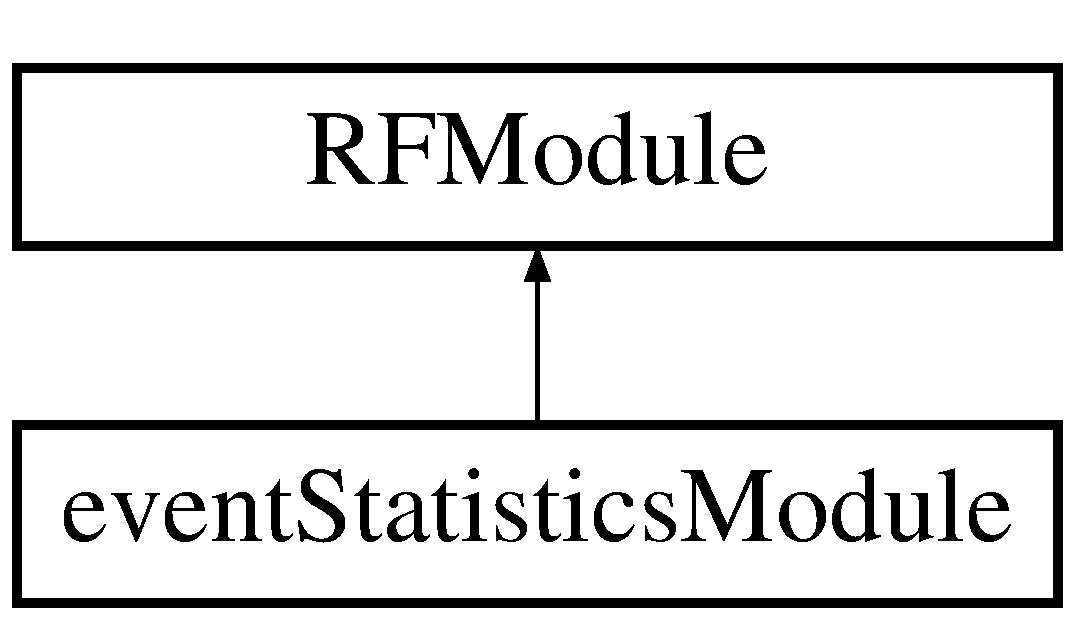
\includegraphics[height=2.000000cm]{classeventStatisticsModule}
\end{center}
\end{figure}
\subsection*{Public Member Functions}
\begin{DoxyCompactItemize}
\item 
\hypertarget{classeventStatisticsModule_a1ca7b5499ca668297430d3976ce3b1d1}{bool {\bfseries configure} (yarp\-::os\-::\-Resource\-Finder \&rf)}\label{classeventStatisticsModule_a1ca7b5499ca668297430d3976ce3b1d1}

\item 
\hypertarget{classeventStatisticsModule_ab11f4b9fdd8ec0d8f3aa0bcb415fef9c}{bool {\bfseries close} ()}\label{classeventStatisticsModule_ab11f4b9fdd8ec0d8f3aa0bcb415fef9c}

\item 
\hypertarget{classeventStatisticsModule_a7e1825323f24dd316be0f7cb7eac80d2}{double {\bfseries get\-Period} ()}\label{classeventStatisticsModule_a7e1825323f24dd316be0f7cb7eac80d2}

\item 
\hypertarget{classeventStatisticsModule_a08194f3ae070dc20ef93a403644ab5a6}{bool {\bfseries update\-Module} ()}\label{classeventStatisticsModule_a08194f3ae070dc20ef93a403644ab5a6}

\end{DoxyCompactItemize}


The documentation for this class was generated from the following files\-:\begin{DoxyCompactItemize}
\item 
/home/aglover/workspace/projects/event\-Driven/src/processing/v\-Analysis/include/event\-Analysis.\-h\item 
/home/aglover/workspace/projects/event\-Driven/src/processing/v\-Analysis/src/event\-Analysis.\-cpp\end{DoxyCompactItemize}

\hypertarget{classemorph_1_1fflowDraw}{\section{emorph\-:\-:fflow\-Draw Class Reference}
\label{classemorph_1_1fflowDraw}\index{emorph\-::fflow\-Draw@{emorph\-::fflow\-Draw}}
}
Inheritance diagram for emorph\-:\-:fflow\-Draw\-:\begin{figure}[H]
\begin{center}
\leavevmode
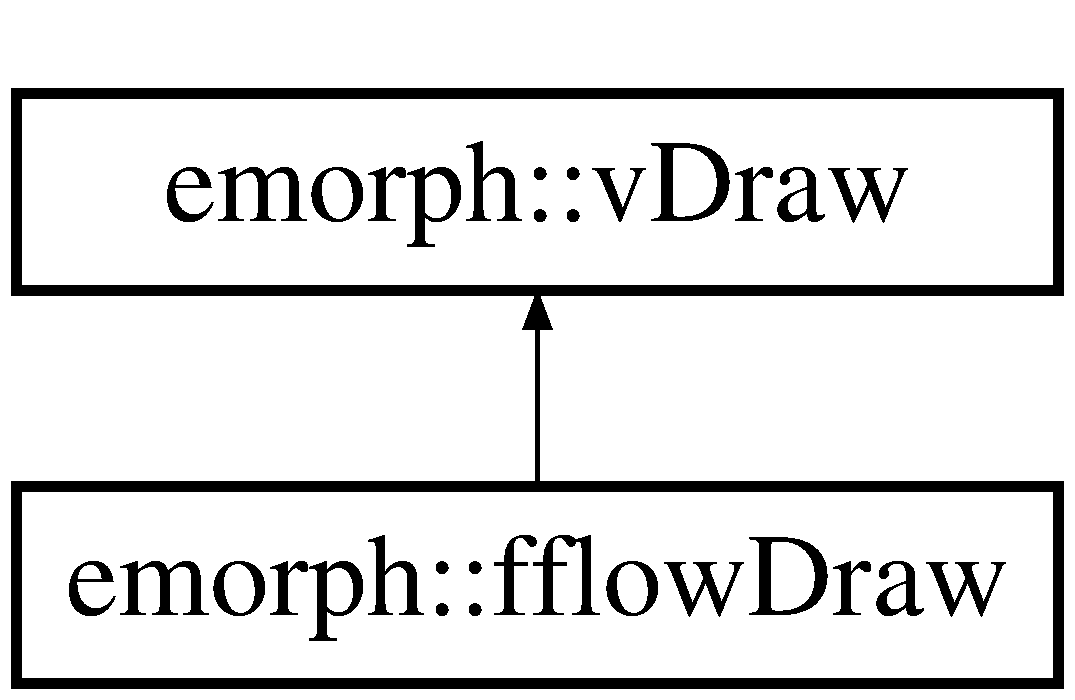
\includegraphics[height=2.000000cm]{classemorph_1_1fflowDraw}
\end{center}
\end{figure}
\subsection*{Public Member Functions}
\begin{DoxyCompactItemize}
\item 
\hypertarget{classemorph_1_1fflowDraw_ae2214e69d31fb9fdcab0e5ba9c8b6f99}{virtual void \hyperlink{classemorph_1_1fflowDraw_ae2214e69d31fb9fdcab0e5ba9c8b6f99}{draw} (cv\-::\-Mat \&image, const \hyperlink{classemorph_1_1vQueue}{emorph\-::v\-Queue} \&e\-Set)}\label{classemorph_1_1fflowDraw_ae2214e69d31fb9fdcab0e5ba9c8b6f99}

\begin{DoxyCompactList}\small\item\em see \hyperlink{classemorph_1_1vDraw}{v\-Draw} \end{DoxyCompactList}\item 
\hypertarget{classemorph_1_1fflowDraw_a742dbd851c4c3a9aca679505571f951d}{virtual std\-::string \hyperlink{classemorph_1_1fflowDraw_a742dbd851c4c3a9aca679505571f951d}{get\-Tag} ()}\label{classemorph_1_1fflowDraw_a742dbd851c4c3a9aca679505571f951d}

\begin{DoxyCompactList}\small\item\em see \hyperlink{classemorph_1_1vDraw}{v\-Draw} \end{DoxyCompactList}\end{DoxyCompactItemize}
\subsection*{Additional Inherited Members}


The documentation for this class was generated from the following files\-:\begin{DoxyCompactItemize}
\item 
/home/aglover/workspace/projects/event\-Driven/src/visualization/v\-Framer/include/i\-Cub/v\-Draw.\-h\item 
/home/aglover/workspace/projects/event\-Driven/src/visualization/v\-Framer/src/v\-Draw.\-cpp\end{DoxyCompactItemize}

\hypertarget{classemorph_1_1fixedDraw}{\section{emorph\-:\-:fixed\-Draw Class Reference}
\label{classemorph_1_1fixedDraw}\index{emorph\-::fixed\-Draw@{emorph\-::fixed\-Draw}}
}
Inheritance diagram for emorph\-:\-:fixed\-Draw\-:\begin{figure}[H]
\begin{center}
\leavevmode
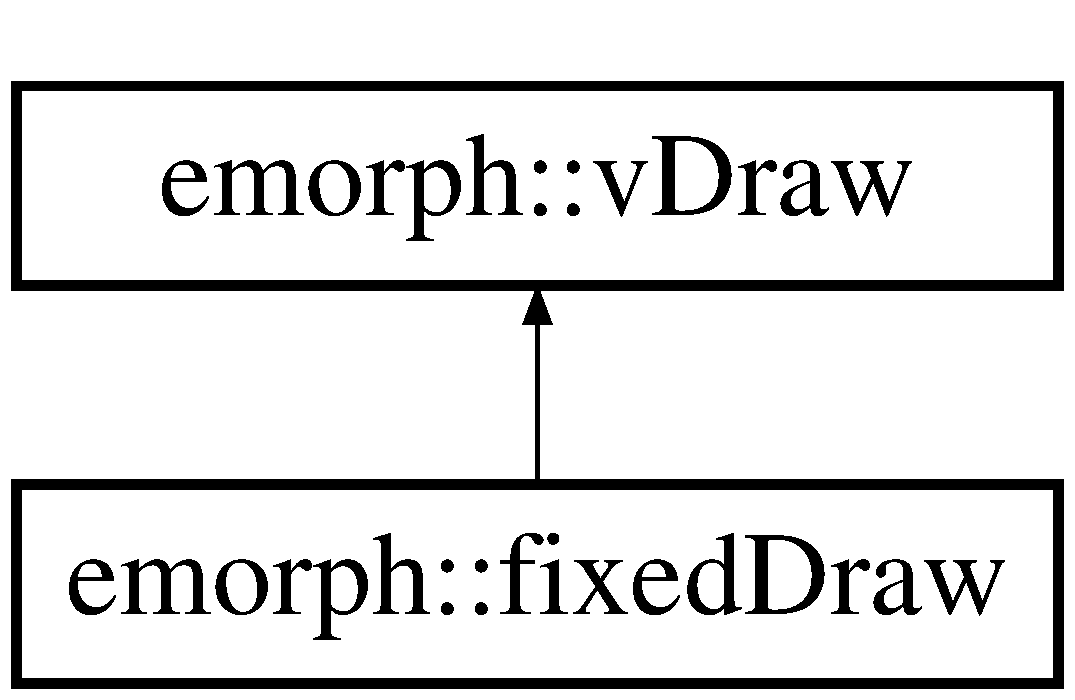
\includegraphics[height=2.000000cm]{classemorph_1_1fixedDraw}
\end{center}
\end{figure}
\subsection*{Public Member Functions}
\begin{DoxyCompactItemize}
\item 
\hypertarget{classemorph_1_1fixedDraw_a6023c32885fc396258fd111a0ed277c6}{virtual void \hyperlink{classemorph_1_1fixedDraw_a6023c32885fc396258fd111a0ed277c6}{draw} (cv\-::\-Mat \&image, const \hyperlink{classemorph_1_1vQueue}{emorph\-::v\-Queue} \&e\-Set)}\label{classemorph_1_1fixedDraw_a6023c32885fc396258fd111a0ed277c6}

\begin{DoxyCompactList}\small\item\em see \hyperlink{classemorph_1_1vDraw}{v\-Draw} \end{DoxyCompactList}\item 
\hypertarget{classemorph_1_1fixedDraw_a3b703843af2824a63c27aacb713d7f50}{virtual std\-::string \hyperlink{classemorph_1_1fixedDraw_a3b703843af2824a63c27aacb713d7f50}{get\-Tag} ()}\label{classemorph_1_1fixedDraw_a3b703843af2824a63c27aacb713d7f50}

\begin{DoxyCompactList}\small\item\em see \hyperlink{classemorph_1_1vDraw}{v\-Draw} \end{DoxyCompactList}\end{DoxyCompactItemize}
\subsection*{Additional Inherited Members}


The documentation for this class was generated from the following files\-:\begin{DoxyCompactItemize}
\item 
/home/aglover/workspace/projects/event\-Driven/src/visualization/v\-Framer/include/i\-Cub/v\-Draw.\-h\item 
/home/aglover/workspace/projects/event\-Driven/src/visualization/v\-Framer/src/v\-Draw.\-cpp\end{DoxyCompactItemize}

\hypertarget{classemorph_1_1flowDraw}{\section{emorph\-:\-:flow\-Draw Class Reference}
\label{classemorph_1_1flowDraw}\index{emorph\-::flow\-Draw@{emorph\-::flow\-Draw}}
}
Inheritance diagram for emorph\-:\-:flow\-Draw\-:\begin{figure}[H]
\begin{center}
\leavevmode
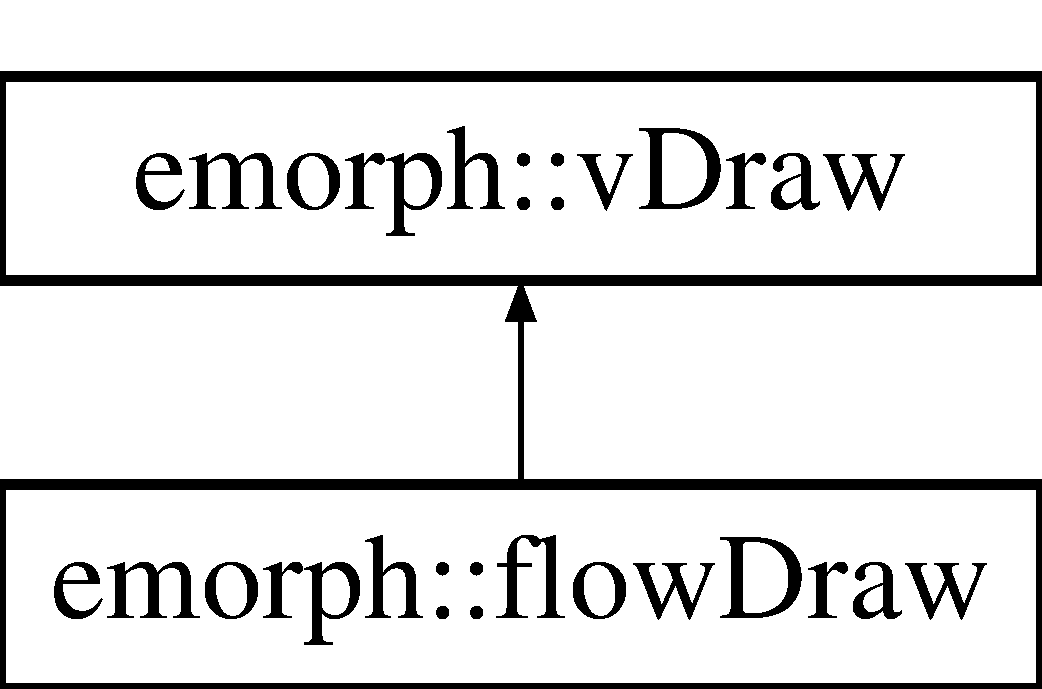
\includegraphics[height=2.000000cm]{classemorph_1_1flowDraw}
\end{center}
\end{figure}
\subsection*{Public Member Functions}
\begin{DoxyCompactItemize}
\item 
\hypertarget{classemorph_1_1flowDraw_a28eeaf6490d8e4f5b334200562d2c31b}{virtual void \hyperlink{classemorph_1_1flowDraw_a28eeaf6490d8e4f5b334200562d2c31b}{draw} (cv\-::\-Mat \&image, const \hyperlink{classemorph_1_1vQueue}{emorph\-::v\-Queue} \&e\-Set)}\label{classemorph_1_1flowDraw_a28eeaf6490d8e4f5b334200562d2c31b}

\begin{DoxyCompactList}\small\item\em see \hyperlink{classemorph_1_1vDraw}{v\-Draw} \end{DoxyCompactList}\item 
\hypertarget{classemorph_1_1flowDraw_a3ba90985c688de6ac753b575e7a322f0}{virtual std\-::string \hyperlink{classemorph_1_1flowDraw_a3ba90985c688de6ac753b575e7a322f0}{get\-Tag} ()}\label{classemorph_1_1flowDraw_a3ba90985c688de6ac753b575e7a322f0}

\begin{DoxyCompactList}\small\item\em see \hyperlink{classemorph_1_1vDraw}{v\-Draw} \end{DoxyCompactList}\end{DoxyCompactItemize}
\subsection*{Additional Inherited Members}


The documentation for this class was generated from the following files\-:\begin{DoxyCompactItemize}
\item 
/home/aglover/workspace/projects/event\-Driven/src/visualization/v\-Framer/include/i\-Cub/v\-Draw.\-h\item 
/home/aglover/workspace/projects/event\-Driven/src/visualization/v\-Framer/src/v\-Draw.\-cpp\end{DoxyCompactItemize}

\hypertarget{classemorph_1_1FlowEvent}{\section{emorph\-:\-:Flow\-Event Class Reference}
\label{classemorph_1_1FlowEvent}\index{emorph\-::\-Flow\-Event@{emorph\-::\-Flow\-Event}}
}
Inheritance diagram for emorph\-:\-:Flow\-Event\-:\begin{figure}[H]
\begin{center}
\leavevmode
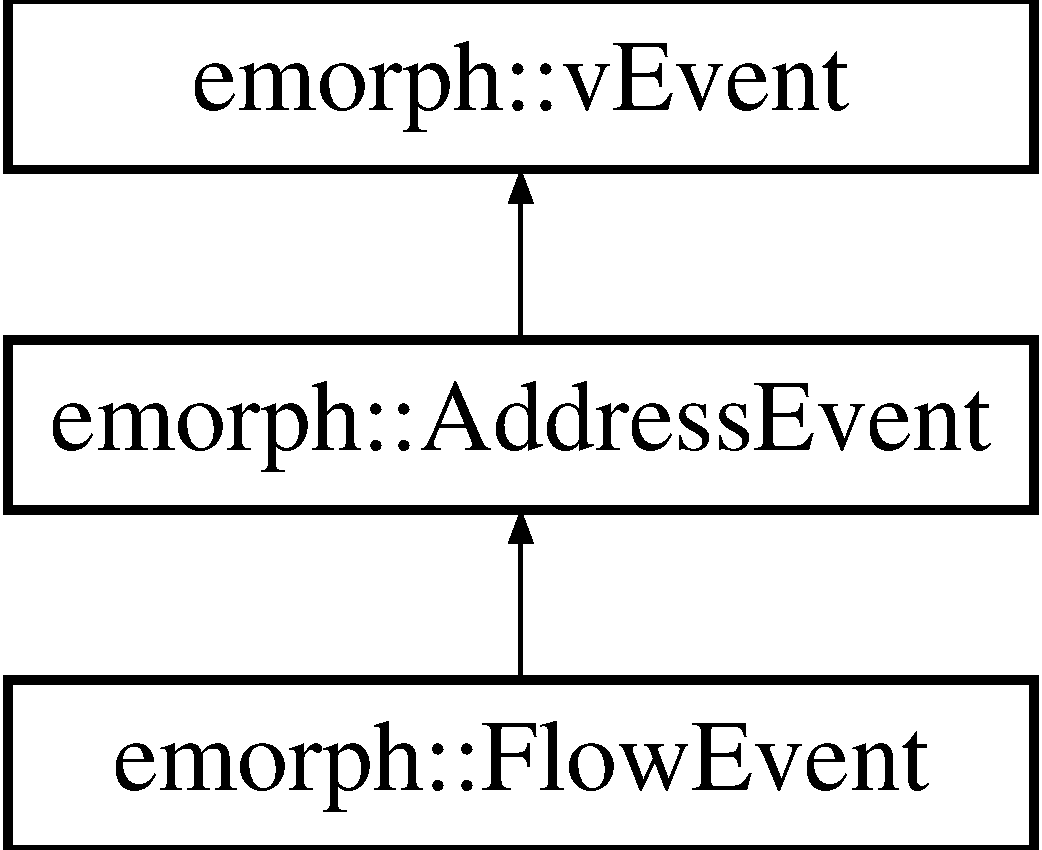
\includegraphics[height=3.000000cm]{classemorph_1_1FlowEvent}
\end{center}
\end{figure}
\subsection*{Public Member Functions}
\begin{DoxyCompactItemize}
\item 
\hypertarget{classemorph_1_1FlowEvent_a263969834e5951fbd45a6cde694acc9d}{virtual std\-::string {\bfseries get\-Type} () const }\label{classemorph_1_1FlowEvent_a263969834e5951fbd45a6cde694acc9d}

\item 
\hypertarget{classemorph_1_1FlowEvent_a200264a57db531501059c85924180bec}{float {\bfseries get\-Vx} () const }\label{classemorph_1_1FlowEvent_a200264a57db531501059c85924180bec}

\item 
\hypertarget{classemorph_1_1FlowEvent_ac8f2dec01073ad7028707f6f24c37453}{float {\bfseries get\-Vy} () const }\label{classemorph_1_1FlowEvent_ac8f2dec01073ad7028707f6f24c37453}

\item 
\hypertarget{classemorph_1_1FlowEvent_acdc608f912f6dacb7d562a57274515a6}{int {\bfseries get\-Death} () const }\label{classemorph_1_1FlowEvent_acdc608f912f6dacb7d562a57274515a6}

\item 
\hypertarget{classemorph_1_1FlowEvent_ad8a37138f5ca4f7939afee340547022a}{void {\bfseries set\-Vx} (float vx)}\label{classemorph_1_1FlowEvent_ad8a37138f5ca4f7939afee340547022a}

\item 
\hypertarget{classemorph_1_1FlowEvent_a818fba434fe4ddbe25e982c4f28c0d87}{void {\bfseries set\-Vy} (float vy)}\label{classemorph_1_1FlowEvent_a818fba434fe4ddbe25e982c4f28c0d87}

\item 
\hypertarget{classemorph_1_1FlowEvent_a3f3fe8eb008bfe643193522d787339ec}{void {\bfseries set\-Death} ()}\label{classemorph_1_1FlowEvent_a3f3fe8eb008bfe643193522d787339ec}

\item 
\hypertarget{classemorph_1_1FlowEvent_acc206219709976fbdfe2792acd0514e8}{{\bfseries Flow\-Event} (const \hyperlink{classemorph_1_1vEvent}{v\-Event} \&event)}\label{classemorph_1_1FlowEvent_acc206219709976fbdfe2792acd0514e8}

\item 
\hypertarget{classemorph_1_1FlowEvent_a8039f858a37816ea202be33201a8e716}{\hyperlink{classemorph_1_1vEvent}{v\-Event} \& {\bfseries operator=} (const \hyperlink{classemorph_1_1vEvent}{v\-Event} \&event)}\label{classemorph_1_1FlowEvent_a8039f858a37816ea202be33201a8e716}

\item 
\hypertarget{classemorph_1_1FlowEvent_abd75e287bbb7706e003fe9c04eaefad7}{virtual \hyperlink{classemorph_1_1vEvent}{v\-Event} $\ast$ {\bfseries clone} ()}\label{classemorph_1_1FlowEvent_abd75e287bbb7706e003fe9c04eaefad7}

\item 
\hypertarget{classemorph_1_1FlowEvent_ab4a83c61991e5524563b3d01f9bc96c5}{bool {\bfseries operator==} (const \hyperlink{classemorph_1_1FlowEvent}{Flow\-Event} \&event)}\label{classemorph_1_1FlowEvent_ab4a83c61991e5524563b3d01f9bc96c5}

\item 
\hypertarget{classemorph_1_1FlowEvent_a16f5cf617614d24c79682179e9e79a58}{bool {\bfseries operator==} (const \hyperlink{classemorph_1_1vEvent}{v\-Event} \&event)}\label{classemorph_1_1FlowEvent_a16f5cf617614d24c79682179e9e79a58}

\item 
\hypertarget{classemorph_1_1FlowEvent_aa7006b5c0b0b94323c7d35244ba060e1}{virtual void {\bfseries encode} (yarp\-::os\-::\-Bottle \&b) const }\label{classemorph_1_1FlowEvent_aa7006b5c0b0b94323c7d35244ba060e1}

\item 
\hypertarget{classemorph_1_1FlowEvent_a77ba93883a630f0a3cb84821df184d1b}{yarp\-::os\-::\-Property {\bfseries get\-Content} () const }\label{classemorph_1_1FlowEvent_a77ba93883a630f0a3cb84821df184d1b}

\item 
\hypertarget{classemorph_1_1FlowEvent_ad416511478fe847398540a483355d863}{virtual bool {\bfseries decode} (const yarp\-::os\-::\-Bottle \&packet, int \&pos)}\label{classemorph_1_1FlowEvent_ad416511478fe847398540a483355d863}

\item 
\hypertarget{classemorph_1_1FlowEvent_ae0fd9eb8662a0db29d3b202073c7c4ea}{virtual int {\bfseries n\-Bytes\-Coded} () const }\label{classemorph_1_1FlowEvent_ae0fd9eb8662a0db29d3b202073c7c4ea}

\end{DoxyCompactItemize}
\subsection*{Protected Attributes}
\begin{DoxyCompactItemize}
\item 
\hypertarget{classemorph_1_1FlowEvent_aa4d42211253a4bce0338abac18942cf4}{float {\bfseries vx}}\label{classemorph_1_1FlowEvent_aa4d42211253a4bce0338abac18942cf4}

\item 
\hypertarget{classemorph_1_1FlowEvent_aad6c4691417beaeff3c64800adc236a3}{float {\bfseries vy}}\label{classemorph_1_1FlowEvent_aad6c4691417beaeff3c64800adc236a3}

\item 
\hypertarget{classemorph_1_1FlowEvent_a772a1742ab4e71afa6bb7fb93c6b6776}{int {\bfseries death}}\label{classemorph_1_1FlowEvent_a772a1742ab4e71afa6bb7fb93c6b6776}

\end{DoxyCompactItemize}
\subsection*{Additional Inherited Members}


The documentation for this class was generated from the following files\-:\begin{DoxyCompactItemize}
\item 
/home/aglover/workspace/projects/event\-Driven/emorph\-\_\-lib/include/i\-Cub/emorph/v\-Codec.\-h\item 
/home/aglover/workspace/projects/event\-Driven/emorph\-\_\-lib/src/v\-Codec.\-cpp\end{DoxyCompactItemize}

\hypertarget{structfpgaStatus}{\section{fpga\-Status Struct Reference}
\label{structfpgaStatus}\index{fpga\-Status@{fpga\-Status}}
}
\subsection*{Public Attributes}
\begin{DoxyCompactItemize}
\item 
\hypertarget{structfpgaStatus_a9cafcfd4e38fa240b31b47611bac3083}{bool {\bfseries crc\-Err}}\label{structfpgaStatus_a9cafcfd4e38fa240b31b47611bac3083}

\item 
\hypertarget{structfpgaStatus_aef80b6cd223b1195b317a70e7f57b58c}{bool {\bfseries bias\-Done}}\label{structfpgaStatus_aef80b6cd223b1195b317a70e7f57b58c}

\item 
\hypertarget{structfpgaStatus_ab37e07a6f39e462634df9d560c0abe45}{bool {\bfseries i2c\-Timeout}}\label{structfpgaStatus_ab37e07a6f39e462634df9d560c0abe45}

\item 
\hypertarget{structfpgaStatus_a01141df5867a1c152efd241a5341cfb7}{bool {\bfseries aps\-Fifo\-Full}}\label{structfpgaStatus_a01141df5867a1c152efd241a5341cfb7}

\item 
\hypertarget{structfpgaStatus_a432c220a53f8a0639cb2b0ef1284ef14}{bool {\bfseries td\-Fifo\-Full}}\label{structfpgaStatus_a432c220a53f8a0639cb2b0ef1284ef14}

\end{DoxyCompactItemize}


The documentation for this struct was generated from the following file\-:\begin{DoxyCompactItemize}
\item 
/home/aglover/workspace/projects/event\-Driven/src/grabbers/zynq\-Grabber/include/i\-Cub/vs\-Ctrl.\-h\end{DoxyCompactItemize}

\hypertarget{classemorph_1_1integralDraw}{\section{emorph\-:\-:integral\-Draw Class Reference}
\label{classemorph_1_1integralDraw}\index{emorph\-::integral\-Draw@{emorph\-::integral\-Draw}}
}
Inheritance diagram for emorph\-:\-:integral\-Draw\-:\begin{figure}[H]
\begin{center}
\leavevmode
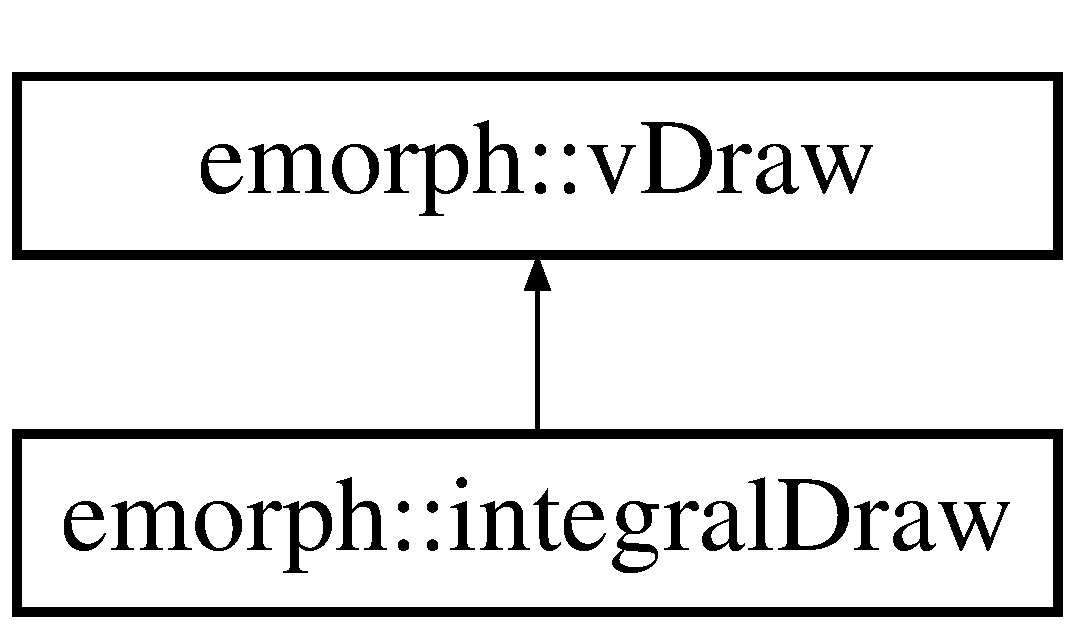
\includegraphics[height=2.000000cm]{classemorph_1_1integralDraw}
\end{center}
\end{figure}
\subsection*{Public Member Functions}
\begin{DoxyCompactItemize}
\item 
\hypertarget{classemorph_1_1integralDraw_a18b3d64b6b81b43c66df4c67955429ff}{virtual void \hyperlink{classemorph_1_1integralDraw_a18b3d64b6b81b43c66df4c67955429ff}{draw} (cv\-::\-Mat \&image, const \hyperlink{classemorph_1_1vQueue}{emorph\-::v\-Queue} \&e\-Set)}\label{classemorph_1_1integralDraw_a18b3d64b6b81b43c66df4c67955429ff}

\begin{DoxyCompactList}\small\item\em see \hyperlink{classemorph_1_1vDraw}{v\-Draw} \end{DoxyCompactList}\item 
\hypertarget{classemorph_1_1integralDraw_a3383c3587a1d99fb3a2352ae4e02371d}{virtual std\-::string \hyperlink{classemorph_1_1integralDraw_a3383c3587a1d99fb3a2352ae4e02371d}{get\-Tag} ()}\label{classemorph_1_1integralDraw_a3383c3587a1d99fb3a2352ae4e02371d}

\begin{DoxyCompactList}\small\item\em see \hyperlink{classemorph_1_1vDraw}{v\-Draw} \end{DoxyCompactList}\end{DoxyCompactItemize}
\subsection*{Additional Inherited Members}


The documentation for this class was generated from the following files\-:\begin{DoxyCompactItemize}
\item 
/home/aglover/workspace/projects/event\-Driven/src/visualization/v\-Framer/include/i\-Cub/v\-Draw.\-h\item 
/home/aglover/workspace/projects/event\-Driven/src/visualization/v\-Framer/src/v\-Draw.\-cpp\end{DoxyCompactItemize}

\hypertarget{classemorph_1_1isoDraw}{\section{emorph\-:\-:iso\-Draw Class Reference}
\label{classemorph_1_1isoDraw}\index{emorph\-::iso\-Draw@{emorph\-::iso\-Draw}}
}
Inheritance diagram for emorph\-:\-:iso\-Draw\-:\begin{figure}[H]
\begin{center}
\leavevmode
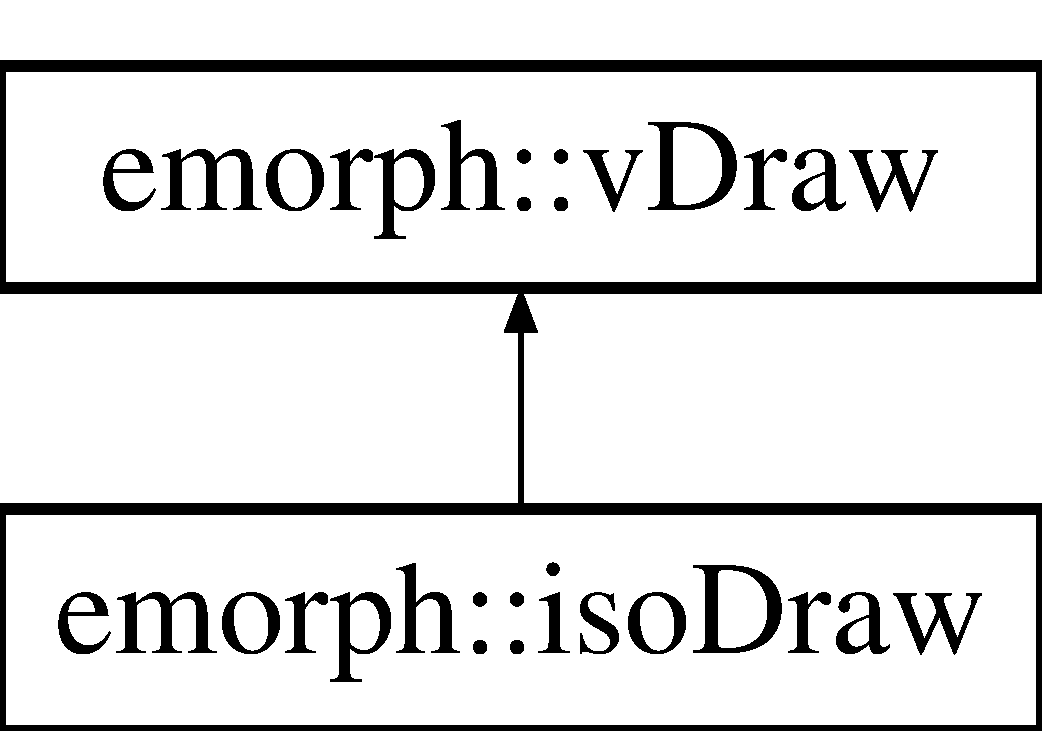
\includegraphics[height=2.000000cm]{classemorph_1_1isoDraw}
\end{center}
\end{figure}
\subsection*{Public Member Functions}
\begin{DoxyCompactItemize}
\item 
\hypertarget{classemorph_1_1isoDraw_aa30dd2dbb7d8f9f087f48582b6772d69}{virtual void \hyperlink{classemorph_1_1isoDraw_aa30dd2dbb7d8f9f087f48582b6772d69}{draw} (cv\-::\-Mat \&image, const \hyperlink{classemorph_1_1vQueue}{emorph\-::v\-Queue} \&e\-Set)}\label{classemorph_1_1isoDraw_aa30dd2dbb7d8f9f087f48582b6772d69}

\begin{DoxyCompactList}\small\item\em see \hyperlink{classemorph_1_1vDraw}{v\-Draw} \end{DoxyCompactList}\item 
\hypertarget{classemorph_1_1isoDraw_a9c62708bc4446b0e55cddb9f47e31d89}{virtual std\-::string \hyperlink{classemorph_1_1isoDraw_a9c62708bc4446b0e55cddb9f47e31d89}{get\-Tag} ()}\label{classemorph_1_1isoDraw_a9c62708bc4446b0e55cddb9f47e31d89}

\begin{DoxyCompactList}\small\item\em see \hyperlink{classemorph_1_1vDraw}{v\-Draw} \end{DoxyCompactList}\end{DoxyCompactItemize}
\subsection*{Additional Inherited Members}


The documentation for this class was generated from the following files\-:\begin{DoxyCompactItemize}
\item 
/home/aglover/workspace/projects/event\-Driven/src/visualization/v\-Framer/include/i\-Cub/v\-Draw.\-h\item 
/home/aglover/workspace/projects/event\-Driven/src/visualization/v\-Framer/src/v\-Draw.\-cpp\end{DoxyCompactItemize}

\hypertarget{classemorph_1_1lifeDraw}{\section{emorph\-:\-:life\-Draw Class Reference}
\label{classemorph_1_1lifeDraw}\index{emorph\-::life\-Draw@{emorph\-::life\-Draw}}
}
Inheritance diagram for emorph\-:\-:life\-Draw\-:\begin{figure}[H]
\begin{center}
\leavevmode
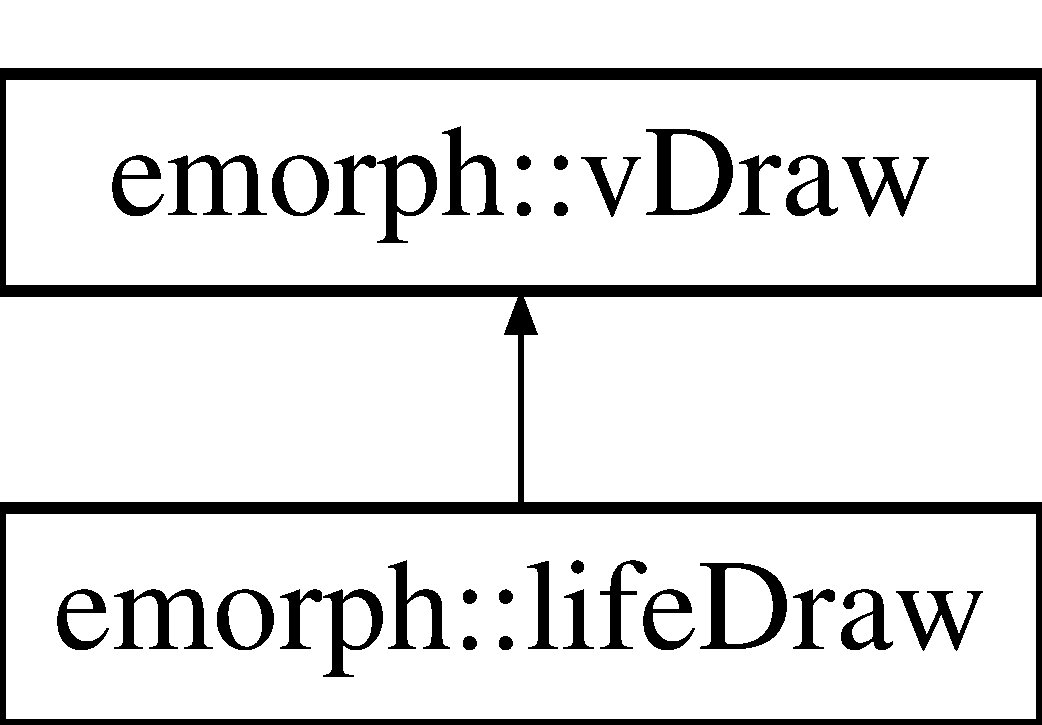
\includegraphics[height=2.000000cm]{classemorph_1_1lifeDraw}
\end{center}
\end{figure}
\subsection*{Public Member Functions}
\begin{DoxyCompactItemize}
\item 
\hypertarget{classemorph_1_1lifeDraw_a2323f8371720151079ab6304d1672853}{virtual void \hyperlink{classemorph_1_1lifeDraw_a2323f8371720151079ab6304d1672853}{draw} (cv\-::\-Mat \&image, const \hyperlink{classemorph_1_1vQueue}{emorph\-::v\-Queue} \&e\-Set)}\label{classemorph_1_1lifeDraw_a2323f8371720151079ab6304d1672853}

\begin{DoxyCompactList}\small\item\em see \hyperlink{classemorph_1_1vDraw}{v\-Draw} \end{DoxyCompactList}\item 
\hypertarget{classemorph_1_1lifeDraw_a11b718fa894541473ea67e0d98331d7a}{virtual std\-::string \hyperlink{classemorph_1_1lifeDraw_a11b718fa894541473ea67e0d98331d7a}{get\-Tag} ()}\label{classemorph_1_1lifeDraw_a11b718fa894541473ea67e0d98331d7a}

\begin{DoxyCompactList}\small\item\em see \hyperlink{classemorph_1_1vDraw}{v\-Draw} \end{DoxyCompactList}\end{DoxyCompactItemize}
\subsection*{Additional Inherited Members}


The documentation for this class was generated from the following files\-:\begin{DoxyCompactItemize}
\item 
/home/aglover/workspace/projects/event\-Driven/src/visualization/v\-Framer/include/i\-Cub/v\-Draw.\-h\item 
/home/aglover/workspace/projects/event\-Driven/src/visualization/v\-Framer/src/v\-Draw.\-cpp\end{DoxyCompactItemize}

\hypertarget{classsaccadeModule}{\section{saccade\-Module Class Reference}
\label{classsaccadeModule}\index{saccade\-Module@{saccade\-Module}}
}
Inheritance diagram for saccade\-Module\-:\begin{figure}[H]
\begin{center}
\leavevmode
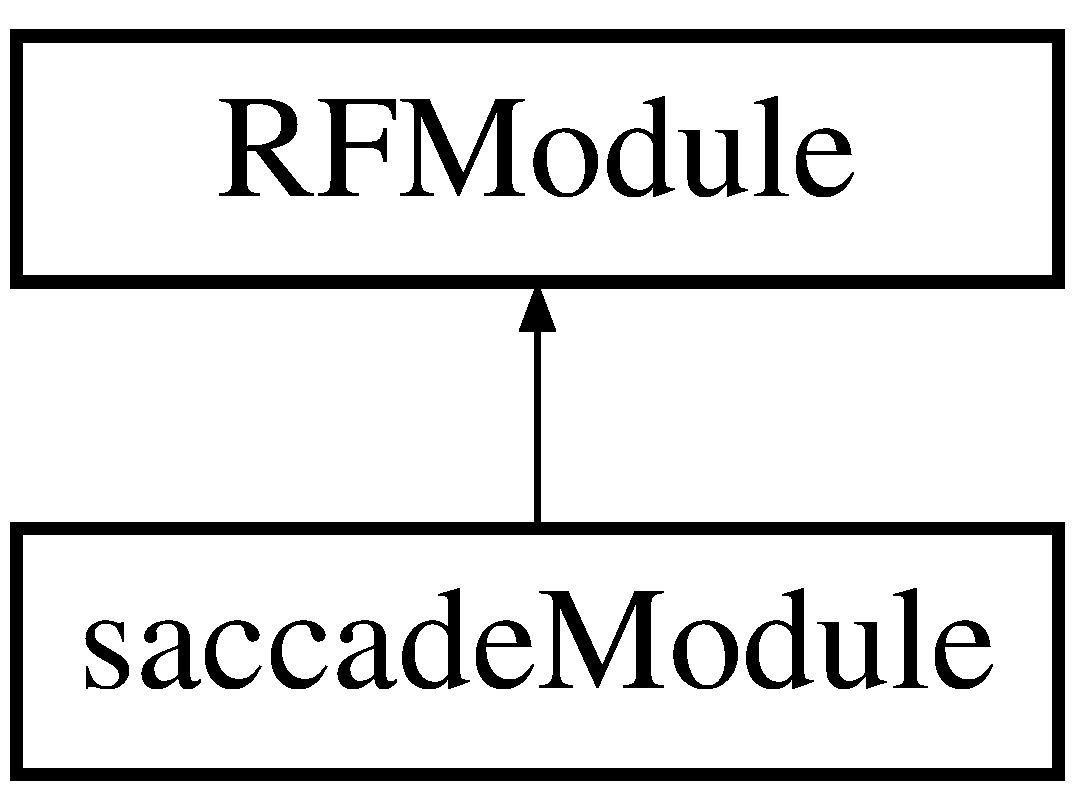
\includegraphics[height=2.000000cm]{classsaccadeModule}
\end{center}
\end{figure}
\subsection*{Public Member Functions}
\begin{DoxyCompactItemize}
\item 
\hypertarget{classsaccadeModule_aad1f5d8c2f33c4c9dadb8e015de9cafc}{virtual bool {\bfseries configure} (yarp\-::os\-::\-Resource\-Finder \&rf)}\label{classsaccadeModule_aad1f5d8c2f33c4c9dadb8e015de9cafc}

\item 
\hypertarget{classsaccadeModule_ac249486e8d00cdb52ec316c5665032ee}{virtual bool {\bfseries interrupt\-Module} ()}\label{classsaccadeModule_ac249486e8d00cdb52ec316c5665032ee}

\item 
\hypertarget{classsaccadeModule_a510ff21af86c5ccf330cf334e63d0f4f}{virtual bool {\bfseries close} ()}\label{classsaccadeModule_a510ff21af86c5ccf330cf334e63d0f4f}

\item 
\hypertarget{classsaccadeModule_a4392d2dc4f60014da07b12772f216430}{virtual bool {\bfseries respond} (const yarp\-::os\-::\-Bottle \&command, yarp\-::os\-::\-Bottle \&reply)}\label{classsaccadeModule_a4392d2dc4f60014da07b12772f216430}

\item 
\hypertarget{classsaccadeModule_a8e603e09181d0cf26b020e6808b9a120}{virtual double {\bfseries get\-Period} ()}\label{classsaccadeModule_a8e603e09181d0cf26b020e6808b9a120}

\item 
\hypertarget{classsaccadeModule_abb6ee7b679476de9ff75d78b75709e9d}{virtual bool {\bfseries update\-Module} ()}\label{classsaccadeModule_abb6ee7b679476de9ff75d78b75709e9d}

\end{DoxyCompactItemize}


The documentation for this class was generated from the following files\-:\begin{DoxyCompactItemize}
\item 
/home/aglover/workspace/projects/event\-Driven/src/movement/autosaccade/include/auto\-Saccade.\-h\item 
/home/aglover/workspace/projects/event\-Driven/src/movement/autosaccade/src/auto\-Saccade.\-cpp\end{DoxyCompactItemize}

\hypertarget{classsendingBuffer}{\section{sending\-Buffer Class Reference}
\label{classsendingBuffer}\index{sending\-Buffer@{sending\-Buffer}}
}
Inheritance diagram for sending\-Buffer\-:\begin{figure}[H]
\begin{center}
\leavevmode
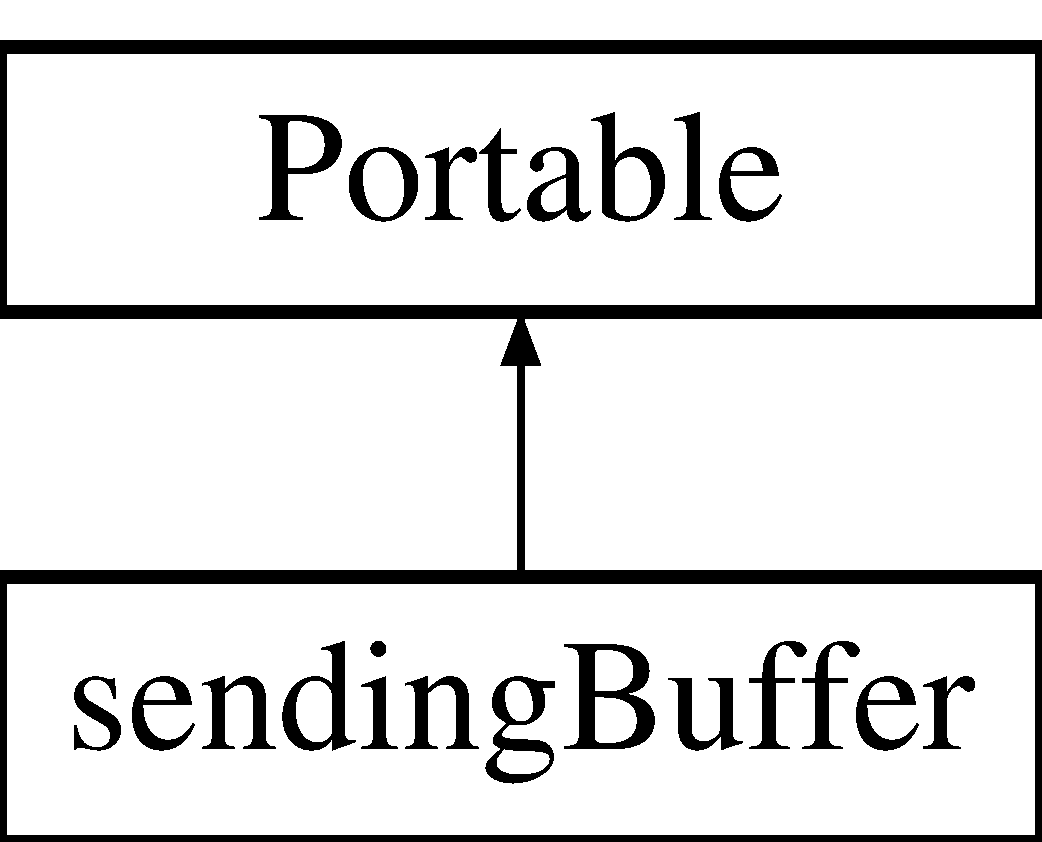
\includegraphics[height=2.000000cm]{classsendingBuffer}
\end{center}
\end{figure}
\subsection*{Public Member Functions}
\begin{DoxyCompactItemize}
\item 
\hypertarget{classsendingBuffer_ab4c1d25d2e85e15f48e06873097deaa2}{{\bfseries sending\-Buffer} (char $\ast$, int)}\label{classsendingBuffer_ab4c1d25d2e85e15f48e06873097deaa2}

\item 
\hypertarget{classsendingBuffer_a40b2e61a078ebe6ea507afd73728f82c}{virtual bool {\bfseries write} (yarp\-::os\-::\-Connection\-Writer \&)}\label{classsendingBuffer_a40b2e61a078ebe6ea507afd73728f82c}

\item 
\hypertarget{classsendingBuffer_ad148ea47f1ef7d56e522909c212ae552}{virtual bool {\bfseries read} (yarp\-::os\-::\-Connection\-Reader \&)}\label{classsendingBuffer_ad148ea47f1ef7d56e522909c212ae552}

\item 
\hypertarget{classsendingBuffer_adf6ced8e177d52765bc8504af4aa0a45}{void {\bfseries set\-\_\-data} (char $\ast$, int)}\label{classsendingBuffer_adf6ced8e177d52765bc8504af4aa0a45}

\item 
\hypertarget{classsendingBuffer_a81ead3fede32e415e1073f31d9bc2f43}{char $\ast$ {\bfseries get\-\_\-packet} ()}\label{classsendingBuffer_a81ead3fede32e415e1073f31d9bc2f43}

\item 
\hypertarget{classsendingBuffer_a76aaef5c8f64d644c04536a9dbb75de6}{int {\bfseries get\-\_\-size\-Of\-Packet} ()}\label{classsendingBuffer_a76aaef5c8f64d644c04536a9dbb75de6}

\end{DoxyCompactItemize}


The documentation for this class was generated from the following files\-:\begin{DoxyCompactItemize}
\item 
/home/aglover/workspace/projects/event\-Driven/src/grabbers/aex\-Grabber/include/i\-Cub/\hyperlink{sending__buffer_8h}{sending\-\_\-buffer.\-h}\item 
/home/aglover/workspace/projects/event\-Driven/src/grabbers/aex\-Grabber/src/sending\-\_\-buffer.\-cpp\end{DoxyCompactItemize}

\hypertarget{structsp2neu__gen__reg}{\section{sp2neu\-\_\-gen\-\_\-reg Struct Reference}
\label{structsp2neu__gen__reg}\index{sp2neu\-\_\-gen\-\_\-reg@{sp2neu\-\_\-gen\-\_\-reg}}
}
\subsection*{Public Attributes}
\begin{DoxyCompactItemize}
\item 
\hypertarget{structsp2neu__gen__reg_a71609646027307154b82fd9323b0a63d}{unsigned int {\bfseries offset}}\label{structsp2neu__gen__reg_a71609646027307154b82fd9323b0a63d}

\item 
\hypertarget{structsp2neu__gen__reg_a3d4d172baa1021c180290c7fa6015ef0}{char {\bfseries rw}}\label{structsp2neu__gen__reg_a3d4d172baa1021c180290c7fa6015ef0}

\item 
\hypertarget{structsp2neu__gen__reg_aabd7dd2a0d1fe28ddfbcf805d3d55d40}{unsigned int {\bfseries data}}\label{structsp2neu__gen__reg_aabd7dd2a0d1fe28ddfbcf805d3d55d40}

\end{DoxyCompactItemize}


The documentation for this struct was generated from the following file\-:\begin{DoxyCompactItemize}
\item 
/home/aglover/workspace/projects/event\-Driven/src/grabbers/zynq\-Grabber/include/i\-Cub/vs\-Ctrl.\-h\end{DoxyCompactItemize}

\hypertarget{classemorph_1_1surfDraw}{\section{emorph\-:\-:surf\-Draw Class Reference}
\label{classemorph_1_1surfDraw}\index{emorph\-::surf\-Draw@{emorph\-::surf\-Draw}}
}
Inheritance diagram for emorph\-:\-:surf\-Draw\-:\begin{figure}[H]
\begin{center}
\leavevmode
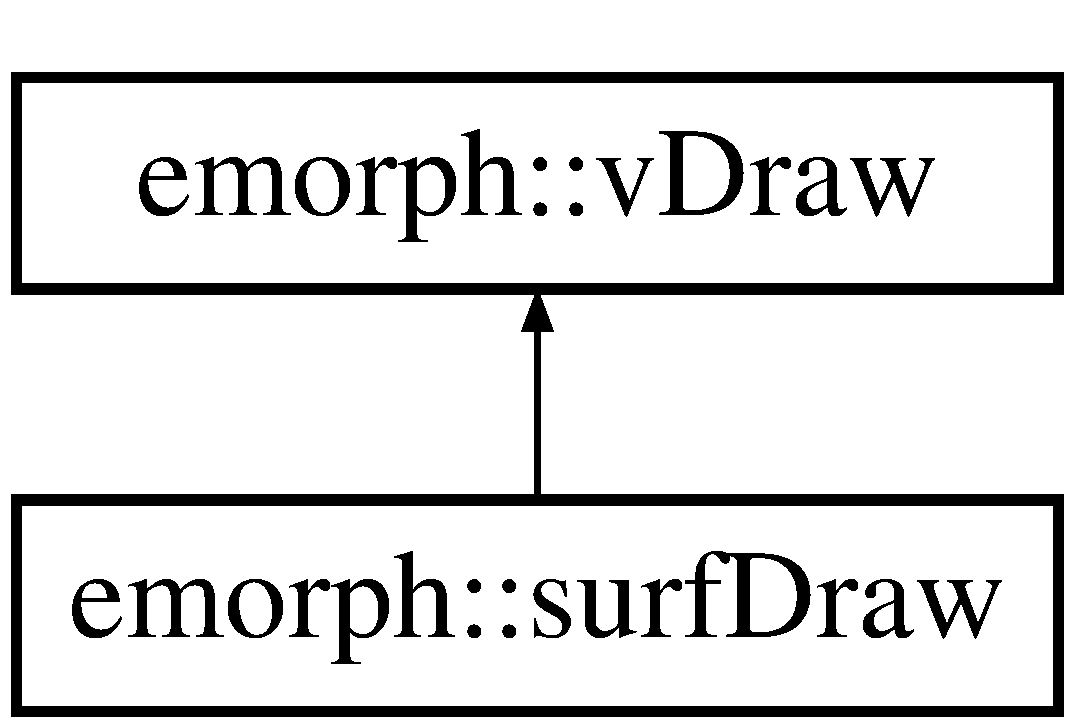
\includegraphics[height=2.000000cm]{classemorph_1_1surfDraw}
\end{center}
\end{figure}
\subsection*{Public Member Functions}
\begin{DoxyCompactItemize}
\item 
\hypertarget{classemorph_1_1surfDraw_a3b448daead5d0bbc9e61fdc0022c0c8b}{virtual void \hyperlink{classemorph_1_1surfDraw_a3b448daead5d0bbc9e61fdc0022c0c8b}{draw} (cv\-::\-Mat \&image, const \hyperlink{classemorph_1_1vQueue}{emorph\-::v\-Queue} \&e\-Set)}\label{classemorph_1_1surfDraw_a3b448daead5d0bbc9e61fdc0022c0c8b}

\begin{DoxyCompactList}\small\item\em see \hyperlink{classemorph_1_1vDraw}{v\-Draw} \end{DoxyCompactList}\item 
\hypertarget{classemorph_1_1surfDraw_aa65dc027fd2d96a01218230525f270e2}{virtual std\-::string \hyperlink{classemorph_1_1surfDraw_aa65dc027fd2d96a01218230525f270e2}{get\-Tag} ()}\label{classemorph_1_1surfDraw_aa65dc027fd2d96a01218230525f270e2}

\begin{DoxyCompactList}\small\item\em see \hyperlink{classemorph_1_1vDraw}{v\-Draw} \end{DoxyCompactList}\end{DoxyCompactItemize}
\subsection*{Static Public Attributes}
\begin{DoxyCompactItemize}
\item 
\hypertarget{classemorph_1_1surfDraw_a05f4f4b2a0840868f1a88dfe3e50ee8e}{static const int {\bfseries gradient} = 100000}\label{classemorph_1_1surfDraw_a05f4f4b2a0840868f1a88dfe3e50ee8e}

\end{DoxyCompactItemize}
\subsection*{Additional Inherited Members}


The documentation for this class was generated from the following files\-:\begin{DoxyCompactItemize}
\item 
/home/aglover/workspace/projects/event\-Driven/src/visualization/v\-Framer/include/i\-Cub/v\-Draw.\-h\item 
/home/aglover/workspace/projects/event\-Driven/src/visualization/v\-Framer/src/v\-Draw.\-cpp\end{DoxyCompactItemize}

\hypertarget{classTrackerPool}{\section{Tracker\-Pool Class Reference}
\label{classTrackerPool}\index{Tracker\-Pool@{Tracker\-Pool}}
}
\subsection*{Public Member Functions}
\begin{DoxyCompactItemize}
\item 
\hypertarget{classTrackerPool_aba64099a18fc9b97eeb5b60f92ca849c}{void {\bfseries set\-Initial\-Params} (double sig\-\_\-x, double sig\-\_\-y, double sig\-\_\-xy, double alpha\-\_\-pos, double alpha\-\_\-shape, bool fixed\-\_\-shape)}\label{classTrackerPool_aba64099a18fc9b97eeb5b60f92ca849c}

\item 
\hypertarget{classTrackerPool_aacfd7b8d8f8d47cf609e6e4ed64bbc1a}{void {\bfseries set\-Decay\-Params} (double decay\-\_\-tau, double Tact, double Tinact, double Tfree, double Tevent, int rate)}\label{classTrackerPool_aacfd7b8d8f8d47cf609e6e4ed64bbc1a}

\item 
\hypertarget{classTrackerPool_a2ae5849c22bc24b688bd5ddf153e9e33}{void {\bfseries set\-Comparison\-Params} (double max\-\_\-dist)}\label{classTrackerPool_a2ae5849c22bc24b688bd5ddf153e9e33}

\item 
\hypertarget{classTrackerPool_a947f58bef9d46a290cb3ea6ec99d5fb8}{void {\bfseries set\-Cluster\-Limit} (int limit)}\label{classTrackerPool_a947f58bef9d46a290cb3ea6ec99d5fb8}

\item 
\hypertarget{classTrackerPool_af54f9236f7d525dde5a14fdee98f92c4}{int {\bfseries update} (\hyperlink{classemorph_1_1AddressEvent}{emorph\-::\-Address\-Event} \&event, std\-::vector$<$ \hyperlink{classemorph_1_1ClusterEventGauss}{emorph\-::\-Cluster\-Event\-Gauss} $>$ \&cl\-Evts)}\label{classTrackerPool_af54f9236f7d525dde5a14fdee98f92c4}

\end{DoxyCompactItemize}
\subsection*{Protected Member Functions}
\begin{DoxyCompactItemize}
\item 
\hypertarget{classTrackerPool_afc17f68023420c6d43ac4b67afa3b14d}{int {\bfseries get\-New\-Tracker} ()}\label{classTrackerPool_afc17f68023420c6d43ac4b67afa3b14d}

\item 
\hypertarget{classTrackerPool_a598259d38408ff2067da4235eab68f9d}{\hyperlink{classemorph_1_1ClusterEventGauss}{emorph\-::\-Cluster\-Event\-Gauss} {\bfseries make\-Event} (int i, int ts)}\label{classTrackerPool_a598259d38408ff2067da4235eab68f9d}

\end{DoxyCompactItemize}
\subsection*{Protected Attributes}
\begin{DoxyCompactItemize}
\item 
\hypertarget{classTrackerPool_a8a8bdb245a4e706de8f9263cc31537cd}{std\-::vector$<$ \hyperlink{classBlobTracker}{Blob\-Tracker} $>$ {\bfseries trackers\-\_\-}}\label{classTrackerPool_a8a8bdb245a4e706de8f9263cc31537cd}

\item 
\hypertarget{classTrackerPool_af542ddb16630e451065d5e3258cd19de}{int {\bfseries nb\-\_\-ev\-\_\-regulate\-\_\-}}\label{classTrackerPool_af542ddb16630e451065d5e3258cd19de}

\item 
\hypertarget{classTrackerPool_a5aed0a9c9621c9fde35034a8b5f58085}{int {\bfseries count\-\_\-}}\label{classTrackerPool_a5aed0a9c9621c9fde35034a8b5f58085}

\item 
\hypertarget{classTrackerPool_ac8ecd306ab6f0562ca2d6231ff367093}{unsigned long int {\bfseries ts\-\_\-last\-\_\-reg\-\_\-}}\label{classTrackerPool_ac8ecd306ab6f0562ca2d6231ff367093}

\item 
\hypertarget{classTrackerPool_abe7439ab3a403e77b56def1ae14ef1c3}{double {\bfseries decay\-\_\-tau}}\label{classTrackerPool_abe7439ab3a403e77b56def1ae14ef1c3}

\item 
\hypertarget{classTrackerPool_aaf7de0a0903e66d7ae07cc11cb6ea072}{double {\bfseries Tact}}\label{classTrackerPool_aaf7de0a0903e66d7ae07cc11cb6ea072}

\item 
\hypertarget{classTrackerPool_a75d2a1d3867ac839d3c24aa26241950e}{double {\bfseries Tinact}}\label{classTrackerPool_a75d2a1d3867ac839d3c24aa26241950e}

\item 
\hypertarget{classTrackerPool_ac75f2360d9bb76e0a6c79b31129c58c5}{double {\bfseries Tfree}}\label{classTrackerPool_ac75f2360d9bb76e0a6c79b31129c58c5}

\item 
\hypertarget{classTrackerPool_a3798b118a9592e75d59ad0d0e5fe438b}{double {\bfseries Tevent}}\label{classTrackerPool_a3798b118a9592e75d59ad0d0e5fe438b}

\item 
\hypertarget{classTrackerPool_ad57d26c00d4329747f59df1b7b24ea3b}{double {\bfseries max\-\_\-dist}}\label{classTrackerPool_ad57d26c00d4329747f59df1b7b24ea3b}

\item 
\hypertarget{classTrackerPool_af83ad39640f58a747253b85046083140}{bool {\bfseries fixed\-\_\-shape\-\_\-}}\label{classTrackerPool_af83ad39640f58a747253b85046083140}

\item 
\hypertarget{classTrackerPool_a6a92ea09387253159839324143b6206a}{double {\bfseries sig\-\_\-x2\-\_\-}}\label{classTrackerPool_a6a92ea09387253159839324143b6206a}

\item 
\hypertarget{classTrackerPool_a3181cb8343949ab80181c9028ae114fa}{double {\bfseries sig\-\_\-y2\-\_\-}}\label{classTrackerPool_a3181cb8343949ab80181c9028ae114fa}

\item 
\hypertarget{classTrackerPool_a9018c85457b2616efe8f718f1602b32a}{double {\bfseries sig\-\_\-xy\-\_\-}}\label{classTrackerPool_a9018c85457b2616efe8f718f1602b32a}

\item 
\hypertarget{classTrackerPool_ad67aaae3b2c777330ccb4abb9bf60884}{double {\bfseries alpha\-\_\-pos}}\label{classTrackerPool_ad67aaae3b2c777330ccb4abb9bf60884}

\item 
\hypertarget{classTrackerPool_ad134dda445a2b5eea2d2101a6e5c2132}{double {\bfseries alpha\-\_\-shape}}\label{classTrackerPool_ad134dda445a2b5eea2d2101a6e5c2132}

\item 
\hypertarget{classTrackerPool_a6c9e6cdff31c0ab40c19f54d30d315cc}{double {\bfseries cluster\-Limit}}\label{classTrackerPool_a6c9e6cdff31c0ab40c19f54d30d315cc}

\item 
\hypertarget{classTrackerPool_a81cc371a7b834bdff0dbaa3601a21d14}{\hyperlink{classemorph_1_1vtsHelper}{emorph\-::vts\-Helper} {\bfseries unwrap}}\label{classTrackerPool_a81cc371a7b834bdff0dbaa3601a21d14}

\end{DoxyCompactItemize}


The documentation for this class was generated from the following files\-:\begin{DoxyCompactItemize}
\item 
/home/aglover/workspace/projects/event\-Driven/src/processing/v\-Cluster/include/tracker\-Pool.\-h\item 
/home/aglover/workspace/projects/event\-Driven/src/processing/v\-Cluster/src/tracker\-Pool.\-cpp\end{DoxyCompactItemize}

\hypertarget{classemorph_1_1vBottle}{\section{emorph\-:\-:v\-Bottle Class Reference}
\label{classemorph_1_1vBottle}\index{emorph\-::v\-Bottle@{emorph\-::v\-Bottle}}
}
Inheritance diagram for emorph\-:\-:v\-Bottle\-:\begin{figure}[H]
\begin{center}
\leavevmode
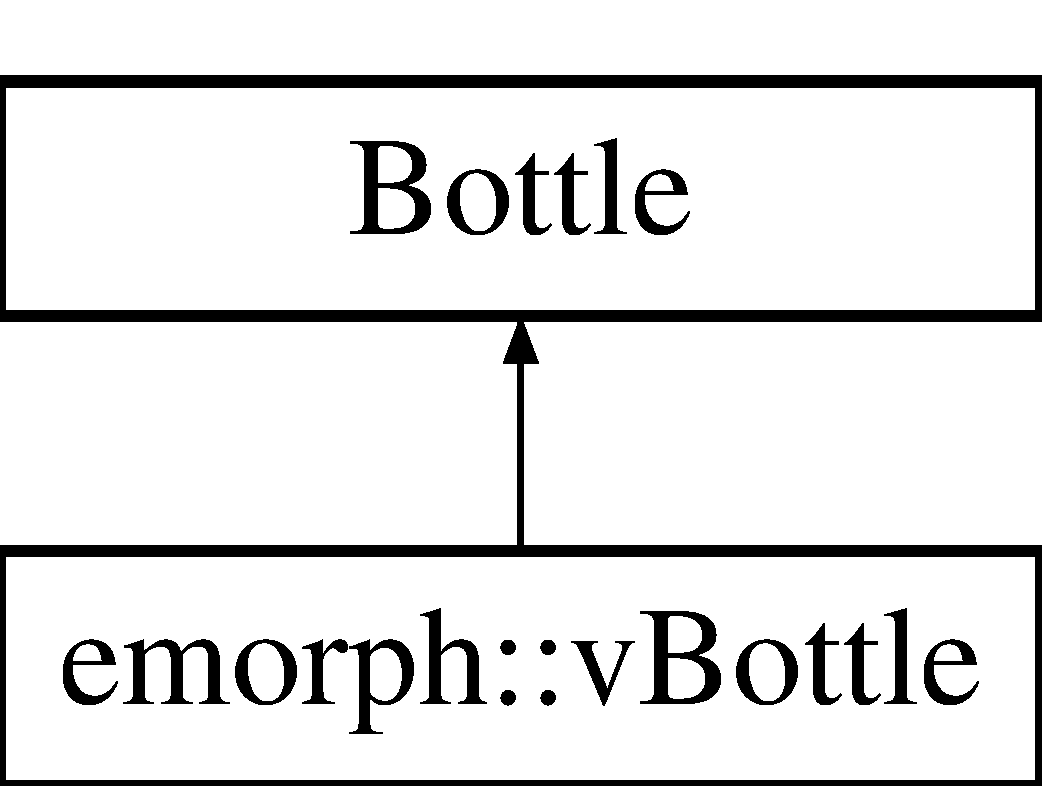
\includegraphics[height=2.000000cm]{classemorph_1_1vBottle}
\end{center}
\end{figure}
\subsection*{Public Member Functions}
\begin{DoxyCompactItemize}
\item 
\hypertarget{classemorph_1_1vBottle_ae4fd194765da088246c407b6c09e336e}{void {\bfseries add\-Event} (\hyperlink{classemorph_1_1vEvent}{emorph\-::v\-Event} \&e)}\label{classemorph_1_1vBottle_ae4fd194765da088246c407b6c09e336e}

\item 
\hypertarget{classemorph_1_1vBottle_a94d820ff09717296c38dd8e4ea3e7a15}{void {\bfseries append} (\hyperlink{classemorph_1_1vBottle}{v\-Bottle} \&eb)}\label{classemorph_1_1vBottle_a94d820ff09717296c38dd8e4ea3e7a15}

\item 
\hypertarget{classemorph_1_1vBottle_a51d19e24f9087a4123f5ef7650ac777a}{{\footnotesize template$<$class T $>$ }\\\hyperlink{classemorph_1_1vQueue}{v\-Queue} {\bfseries get} ()}\label{classemorph_1_1vBottle_a51d19e24f9087a4123f5ef7650ac777a}

\item 
\hypertarget{classemorph_1_1vBottle_af8006479b9ef748f0ff6e441284a46c7}{{\footnotesize template$<$class T $>$ }\\void {\bfseries addtoendof} (\hyperlink{classemorph_1_1vQueue}{v\-Queue} \&q)}\label{classemorph_1_1vBottle_af8006479b9ef748f0ff6e441284a46c7}

\item 
\hypertarget{classemorph_1_1vBottle_a450019145cdb646901e4f5ac46a9f72e}{{\footnotesize template$<$class T $>$ }\\\hyperlink{classemorph_1_1vQueue}{v\-Queue} {\bfseries get\-Sorted} ()}\label{classemorph_1_1vBottle_a450019145cdb646901e4f5ac46a9f72e}

\item 
\hypertarget{classemorph_1_1vBottle_a1820eeaa7576d0f7bcf0de6420d40435}{\hyperlink{classemorph_1_1vQueue}{v\-Queue} {\bfseries get\-All} ()}\label{classemorph_1_1vBottle_a1820eeaa7576d0f7bcf0de6420d40435}

\item 
\hypertarget{classemorph_1_1vBottle_af4df9387ad493ec4451e1f5c2232ce0b}{\hyperlink{classemorph_1_1vQueue}{v\-Queue} {\bfseries get\-All\-Sorted} ()}\label{classemorph_1_1vBottle_af4df9387ad493ec4451e1f5c2232ce0b}

\end{DoxyCompactItemize}


The documentation for this class was generated from the following files\-:\begin{DoxyCompactItemize}
\item 
/home/aglover/workspace/projects/event\-Driven/emorph\-\_\-lib/include/i\-Cub/emorph/v\-Bottle.\-h\item 
/home/aglover/workspace/projects/event\-Driven/emorph\-\_\-lib/src/v\-Bottle.\-cpp\end{DoxyCompactItemize}

\hypertarget{classemorph_1_1vBottleMimic}{\section{emorph\-:\-:v\-Bottle\-Mimic Class Reference}
\label{classemorph_1_1vBottleMimic}\index{emorph\-::v\-Bottle\-Mimic@{emorph\-::v\-Bottle\-Mimic}}
}
Inheritance diagram for emorph\-:\-:v\-Bottle\-Mimic\-:\begin{figure}[H]
\begin{center}
\leavevmode
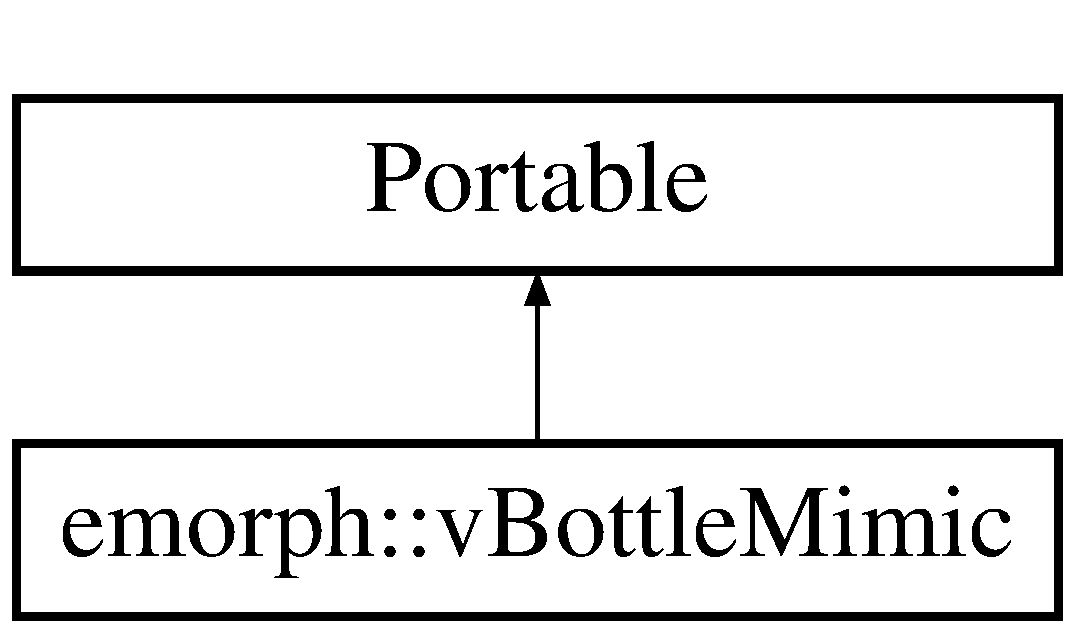
\includegraphics[height=2.000000cm]{classemorph_1_1vBottleMimic}
\end{center}
\end{figure}
\subsection*{Public Member Functions}
\begin{DoxyCompactItemize}
\item 
\hypertarget{classemorph_1_1vBottleMimic_ace7355fd2d178bbd899694ba81e3222b}{void {\bfseries setdata} (const char $\ast$datablock, unsigned int datalength)}\label{classemorph_1_1vBottleMimic_ace7355fd2d178bbd899694ba81e3222b}

\item 
\hypertarget{classemorph_1_1vBottleMimic_ae97dabc0425bae4aaaa1679100e36885}{virtual bool {\bfseries read} (yarp\-::os\-::\-Connection\-Reader \&connection)}\label{classemorph_1_1vBottleMimic_ae97dabc0425bae4aaaa1679100e36885}

\item 
\hypertarget{classemorph_1_1vBottleMimic_af930ab7e4e14992dd2182b4c46e2a5d1}{virtual bool {\bfseries write} (yarp\-::os\-::\-Connection\-Writer \&connection)}\label{classemorph_1_1vBottleMimic_af930ab7e4e14992dd2182b4c46e2a5d1}

\end{DoxyCompactItemize}


The documentation for this class was generated from the following file\-:\begin{DoxyCompactItemize}
\item 
/home/aglover/workspace/projects/event\-Driven/emorph\-\_\-lib/include/i\-Cub/emorph/v\-Bottle.\-h\end{DoxyCompactItemize}

\hypertarget{classvCircleModule}{\section{v\-Circle\-Module Class Reference}
\label{classvCircleModule}\index{v\-Circle\-Module@{v\-Circle\-Module}}
}
Inheritance diagram for v\-Circle\-Module\-:\begin{figure}[H]
\begin{center}
\leavevmode
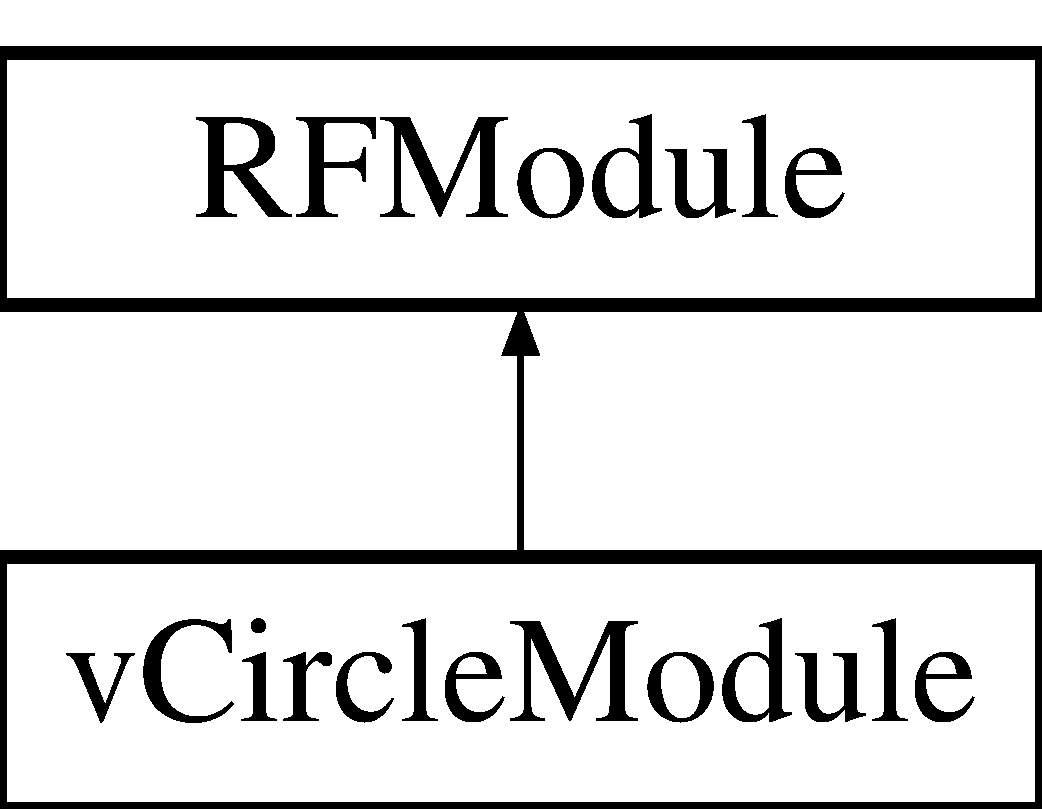
\includegraphics[height=2.000000cm]{classvCircleModule}
\end{center}
\end{figure}
\subsection*{Public Member Functions}
\begin{DoxyCompactItemize}
\item 
\hypertarget{classvCircleModule_a4b1534c8acd2a20a874b1e3fb2f2bbbf}{virtual bool {\bfseries configure} (yarp\-::os\-::\-Resource\-Finder \&rf)}\label{classvCircleModule_a4b1534c8acd2a20a874b1e3fb2f2bbbf}

\item 
\hypertarget{classvCircleModule_a48b6db38d3e64e47df8dc276844d7bd2}{virtual bool {\bfseries interrupt\-Module} ()}\label{classvCircleModule_a48b6db38d3e64e47df8dc276844d7bd2}

\item 
\hypertarget{classvCircleModule_a7d2220bd00b1e7081ec104a4c208f8d7}{virtual bool {\bfseries close} ()}\label{classvCircleModule_a7d2220bd00b1e7081ec104a4c208f8d7}

\item 
\hypertarget{classvCircleModule_abf28f9b5e2f01acf56bf825f1fcc2e01}{virtual double {\bfseries get\-Period} ()}\label{classvCircleModule_abf28f9b5e2f01acf56bf825f1fcc2e01}

\item 
\hypertarget{classvCircleModule_a176830c8a500b828c3f50d87b5e2d671}{virtual bool {\bfseries update\-Module} ()}\label{classvCircleModule_a176830c8a500b828c3f50d87b5e2d671}

\end{DoxyCompactItemize}


The documentation for this class was generated from the following files\-:\begin{DoxyCompactItemize}
\item 
/home/aglover/workspace/projects/event\-Driven/src/processing/v\-Circle/include/v\-Circle\-Module.\-h\item 
/home/aglover/workspace/projects/event\-Driven/src/processing/v\-Circle/src/v\-Circle\-Module.\-cpp\end{DoxyCompactItemize}

\hypertarget{classvCircleMultiSize}{\section{v\-Circle\-Multi\-Size Class Reference}
\label{classvCircleMultiSize}\index{v\-Circle\-Multi\-Size@{v\-Circle\-Multi\-Size}}
}
\subsection*{Public Member Functions}
\begin{DoxyCompactItemize}
\item 
\hypertarget{classvCircleMultiSize_a366696892bbe5b156211e15c863eff26}{{\bfseries v\-Circle\-Multi\-Size} (std\-::string q\-Type=\char`\"{}Fixed\char`\"{}, int q\-Length=2000, int r\-Low=8, int r\-High=38, bool directed=true, bool parallel=false, int height=128, int width=128)}\label{classvCircleMultiSize_a366696892bbe5b156211e15c863eff26}

\item 
\hypertarget{classvCircleMultiSize_aae2be51a17ecc1dad90d75a1f60a50ee}{void {\bfseries add\-Queue} (\hyperlink{classemorph_1_1vQueue}{emorph\-::v\-Queue} \&additions)}\label{classvCircleMultiSize_aae2be51a17ecc1dad90d75a1f60a50ee}

\item 
\hypertarget{classvCircleMultiSize_a661f425152259951f87167bdcd53caaf}{double {\bfseries get\-Obs} (int \&x, int \&y, int \&r)}\label{classvCircleMultiSize_a661f425152259951f87167bdcd53caaf}

\item 
\hypertarget{classvCircleMultiSize_a1dc2c81da6abc8aaaaedf0d169ad9671}{yarp\-::sig\-::\-Image\-Of\\*
$<$ yarp\-::sig\-::\-Pixel\-Bgr $>$ {\bfseries make\-Debug\-Image} ()}\label{classvCircleMultiSize_a1dc2c81da6abc8aaaaedf0d169ad9671}

\end{DoxyCompactItemize}


The documentation for this class was generated from the following files\-:\begin{DoxyCompactItemize}
\item 
/home/aglover/workspace/projects/event\-Driven/src/processing/v\-Circle/include/v\-Circle\-Observer.\-h\item 
/home/aglover/workspace/projects/event\-Driven/src/processing/v\-Circle/src/v\-Circle\-Observer.\-cpp\end{DoxyCompactItemize}

\hypertarget{classvCircleReader}{\section{v\-Circle\-Reader Class Reference}
\label{classvCircleReader}\index{v\-Circle\-Reader@{v\-Circle\-Reader}}
}


{\ttfamily \#include $<$v\-Circle\-Module.\-h$>$}

Inheritance diagram for v\-Circle\-Reader\-:\begin{figure}[H]
\begin{center}
\leavevmode
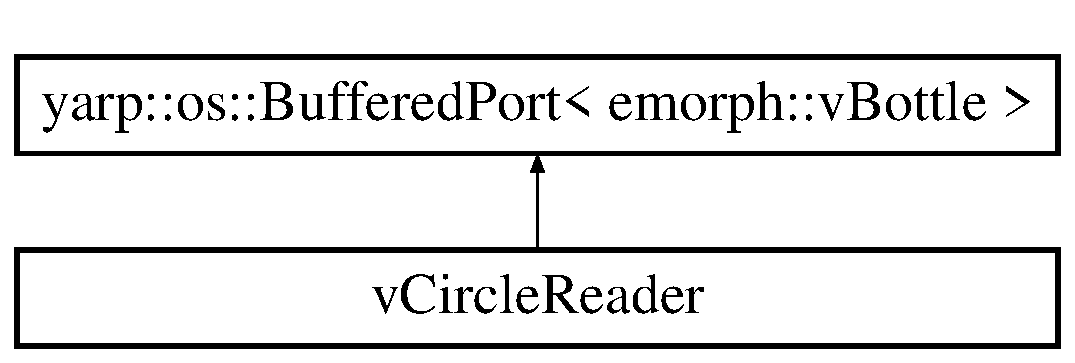
\includegraphics[height=2.000000cm]{classvCircleReader}
\end{center}
\end{figure}
\subsection*{Public Member Functions}
\begin{DoxyCompactItemize}
\item 
\hypertarget{classvCircleReader_aeea09b1b0a4f6ca43362430e2b7c13f3}{bool {\bfseries open} (const std\-::string \&name, bool strictness=false)}\label{classvCircleReader_aeea09b1b0a4f6ca43362430e2b7c13f3}

\item 
\hypertarget{classvCircleReader_a963ecb3d9e66c9a6d0dd3deb0107d333}{void {\bfseries close} ()}\label{classvCircleReader_a963ecb3d9e66c9a6d0dd3deb0107d333}

\item 
\hypertarget{classvCircleReader_adb1e49808d1ff24b38e68ad3c706d87a}{void {\bfseries interrupt} ()}\label{classvCircleReader_adb1e49808d1ff24b38e68ad3c706d87a}

\item 
\hypertarget{classvCircleReader_a413308d9f280c2e5040e0b10fc9ccd5b}{void {\bfseries on\-Read} (\hyperlink{classemorph_1_1vBottle}{emorph\-::v\-Bottle} \&in\-Bot)}\label{classvCircleReader_a413308d9f280c2e5040e0b10fc9ccd5b}

\item 
\hypertarget{classvCircleReader_a13856006b160d12edb43f0130f5a0987}{bool {\bfseries set\-Data\-Writer} (std\-::string datafilename)}\label{classvCircleReader_a13856006b160d12edb43f0130f5a0987}

\end{DoxyCompactItemize}
\subsection*{Public Attributes}
\begin{DoxyCompactItemize}
\item 
\hypertarget{classvCircleReader_a7b0ae9557cbe36e72339cc7479d99833}{\hyperlink{classvCircleTracker}{v\-Circle\-Tracker} {\bfseries circle\-Tracker}}\label{classvCircleReader_a7b0ae9557cbe36e72339cc7479d99833}

\item 
\hypertarget{classvCircleReader_a8aff6c9feaa9806894f739e7c62b8c69}{\hyperlink{classvCircleMultiSize}{v\-Circle\-Multi\-Size} $\ast$ {\bfseries c\-Observer}}\label{classvCircleReader_a8aff6c9feaa9806894f739e7c62b8c69}

\item 
\hypertarget{classvCircleReader_abb1da4c345eb519b695927d12f2f1ec8}{double {\bfseries inlier\-Threshold}}\label{classvCircleReader_abb1da4c345eb519b695927d12f2f1ec8}

\item 
\hypertarget{classvCircleReader_a2a026b4c43ab7e721b6089b4118767a4}{bool {\bfseries hough}}\label{classvCircleReader_a2a026b4c43ab7e721b6089b4118767a4}

\item 
\hypertarget{classvCircleReader_a0bcf9e8b5c28b2ea048ab75c4213023e}{double {\bfseries timecounter}}\label{classvCircleReader_a0bcf9e8b5c28b2ea048ab75c4213023e}

\end{DoxyCompactItemize}


\subsection{Detailed Description}
This module uses the Hough transform at several radii to detect circles in the event-\/driven data stream.\hypertarget{group__aexGrabber_parameters_sec}{}\subsection{Parameters}\label{group__aexGrabber_parameters_sec}

\begin{DoxyItemize}
\item {\ttfamily name} {\ttfamily v\-Circle} \par
 set the root string for port naming e.\-g. /v\-Circle/v\-Bottle\-:i
\item {\ttfamily strict} {\ttfamily true} $\vert$ false \par
 set port writing strictness of this module
\item {\ttfamily hough\-Type} {\ttfamily directed} $\vert$ full \par
 set the Hough transform method\-: full (standard) or directed
\item {\ttfamily q\-Type} {\ttfamily Fixed} $\vert$ Lifetime \par
 set the v\-Queue method using a fixed size or using the event-\/lifetime
\item {\ttfamily inlier\-Threshold} {\ttfamily 25} \par
 set the threshold on positive circle detection
\end{DoxyItemize}\hypertarget{group__aexGrabber_portsa_sec}{}\subsection{Ports Accessed}\label{group__aexGrabber_portsa_sec}
\hypertarget{group__aexGrabber_portsc_sec}{}\subsection{Ports Created}\label{group__aexGrabber_portsc_sec}
{\bfseries  Input ports }


\begin{DoxyItemize}
\item {\ttfamily /v\-Circle/v\-Bottle}\-:i \par
 input port for v\-Bottles containing Address\-Events or Flow\-Events
\end{DoxyItemize}

{\bfseries  Output ports }


\begin{DoxyItemize}
\item {\ttfamily /v\-Circle/v\-Bottle}\-:o \par
 appends the input bottle with circle detection events
\item {\ttfamily /v\-Circle/debug}\-:o \par
 a yarp image visualising the hough space (slows down detection rate)
\end{DoxyItemize}\hypertarget{group__aexGrabber_example_sec}{}\subsection{Example Instantiation of the Module}\label{group__aexGrabber_example_sec}
{\ttfamily aex\-Grabber --name v\-Circle --strict true --hough\-Type directed -- q\-Type Fixed --inlier\-Threshold 25 }

\begin{DoxyAuthor}{Author}
Arren Glover 
\end{DoxyAuthor}


The documentation for this class was generated from the following file\-:\begin{DoxyCompactItemize}
\item 
/home/aglover/workspace/projects/event\-Driven/src/processing/v\-Circle/include/v\-Circle\-Module.\-h\end{DoxyCompactItemize}

\hypertarget{classvCircleThread}{\section{v\-Circle\-Thread Class Reference}
\label{classvCircleThread}\index{v\-Circle\-Thread@{v\-Circle\-Thread}}
}


The \hyperlink{classvCircleThread}{v\-Circle\-Thread} class performs a circular Hough transform.  




{\ttfamily \#include $<$v\-Circle\-Observer.\-h$>$}

Inheritance diagram for v\-Circle\-Thread\-:\begin{figure}[H]
\begin{center}
\leavevmode
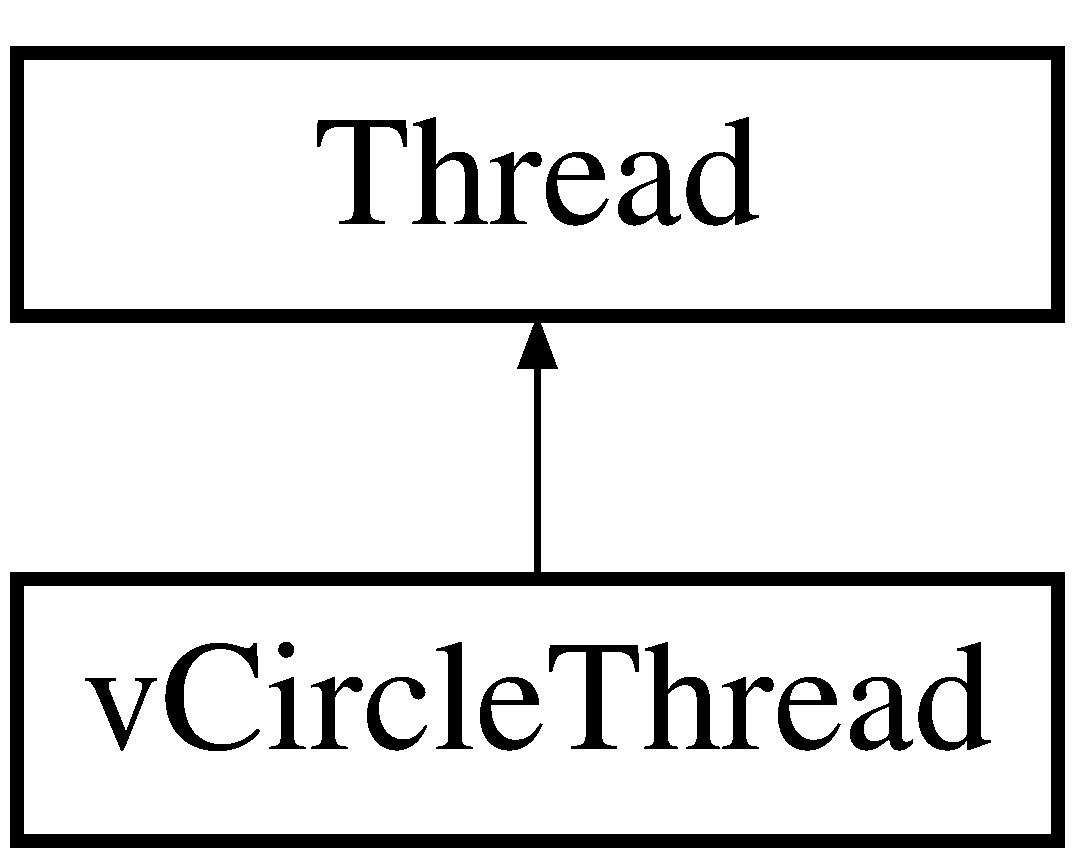
\includegraphics[height=2.000000cm]{classvCircleThread}
\end{center}
\end{figure}
\subsection*{Public Member Functions}
\begin{DoxyCompactItemize}
\item 
\hyperlink{classvCircleThread_ab1202e2b0cebcad0ddbe6033e3742d4e}{v\-Circle\-Thread} (int R, bool directed, bool parallel=false, int height=128, int width=128)
\begin{DoxyCompactList}\small\item\em \hyperlink{classvCircleThread}{v\-Circle\-Thread} constructor \end{DoxyCompactList}\item 
double \hyperlink{classvCircleThread_a692a1066ee63c2716998fcb3a7aa513d}{get\-Score} ()
\begin{DoxyCompactList}\small\item\em get\-Score get the maximum strength in Hough space \end{DoxyCompactList}\item 
int \hyperlink{classvCircleThread_a0feac9f937bfeecc2dc0b015f9e8161c}{get\-X} ()
\begin{DoxyCompactList}\small\item\em get\-X get the maximum strength location \end{DoxyCompactList}\item 
int \hyperlink{classvCircleThread_a4f39898c53c3178b84b28c8cc33ec352}{get\-Y} ()
\begin{DoxyCompactList}\small\item\em get\-Y get the maximum strength location \end{DoxyCompactList}\item 
int \hyperlink{classvCircleThread_a024aa1ad0a7855fad146425c80feadb0}{get\-R} ()
\begin{DoxyCompactList}\small\item\em get\-R return the radius of the circle to be detected \end{DoxyCompactList}\item 
void \hyperlink{classvCircleThread_a97d976b1db541ddaf19f4688212cb05b}{process} (\hyperlink{classemorph_1_1vQueue}{emorph\-::v\-Queue} \&adds, \hyperlink{classemorph_1_1vQueue}{emorph\-::v\-Queue} \&subs)
\begin{DoxyCompactList}\small\item\em process update the Hough transform (threaded or non-\/threaded) \end{DoxyCompactList}\item 
\hypertarget{classvCircleThread_a0d32749f12d2d93ff0d9ccdf37422ccf}{void \hyperlink{classvCircleThread_a0d32749f12d2d93ff0d9ccdf37422ccf}{waitfordone} ()}\label{classvCircleThread_a0d32749f12d2d93ff0d9ccdf37422ccf}

\begin{DoxyCompactList}\small\item\em waitfordone wait for computation to finish if threaded \end{DoxyCompactList}\item 
yarp\-::sig\-::\-Image\-Of\\*
$<$ yarp\-::sig\-::\-Pixel\-Bgr $>$ \hyperlink{classvCircleThread_a4849d1320c36b9ef7efafda71bc612c9}{make\-Debug\-Image} ()
\begin{DoxyCompactList}\small\item\em make\-Debug\-Image create an image visualising the Hough space \end{DoxyCompactList}\end{DoxyCompactItemize}


\subsection{Detailed Description}
The \hyperlink{classvCircleThread}{v\-Circle\-Thread} class performs a circular Hough transform. 

The class gives the maximal location and strength of a circular shape of a single given radius. The class can use the directed transform and can be threaded for use on multi-\/core systems. 

\subsection{Constructor \& Destructor Documentation}
\hypertarget{classvCircleThread_ab1202e2b0cebcad0ddbe6033e3742d4e}{\index{v\-Circle\-Thread@{v\-Circle\-Thread}!v\-Circle\-Thread@{v\-Circle\-Thread}}
\index{v\-Circle\-Thread@{v\-Circle\-Thread}!vCircleThread@{v\-Circle\-Thread}}
\subsubsection[{v\-Circle\-Thread}]{\setlength{\rightskip}{0pt plus 5cm}v\-Circle\-Thread\-::v\-Circle\-Thread (
\begin{DoxyParamCaption}
\item[{int}]{R, }
\item[{bool}]{directed, }
\item[{bool}]{parallel = {\ttfamily false}, }
\item[{int}]{height = {\ttfamily 128}, }
\item[{int}]{width = {\ttfamily 128}}
\end{DoxyParamCaption}
)}}\label{classvCircleThread_ab1202e2b0cebcad0ddbe6033e3742d4e}


\hyperlink{classvCircleThread}{v\-Circle\-Thread} constructor 


\begin{DoxyParams}{Parameters}
{\em R} & circle radius \\
\hline
{\em directed} & use directed Hough transform \\
\hline
{\em parallel} & use a separate thread for computation \\
\hline
{\em height} & sensor height \\
\hline
{\em width} & sensor width \\
\hline
\end{DoxyParams}


\subsection{Member Function Documentation}
\hypertarget{classvCircleThread_a024aa1ad0a7855fad146425c80feadb0}{\index{v\-Circle\-Thread@{v\-Circle\-Thread}!get\-R@{get\-R}}
\index{get\-R@{get\-R}!vCircleThread@{v\-Circle\-Thread}}
\subsubsection[{get\-R}]{\setlength{\rightskip}{0pt plus 5cm}int v\-Circle\-Thread\-::get\-R (
\begin{DoxyParamCaption}
{}
\end{DoxyParamCaption}
)\hspace{0.3cm}{\ttfamily [inline]}}}\label{classvCircleThread_a024aa1ad0a7855fad146425c80feadb0}


get\-R return the radius of the circle to be detected 

\begin{DoxyReturn}{Returns}
the radius R 
\end{DoxyReturn}
\hypertarget{classvCircleThread_a692a1066ee63c2716998fcb3a7aa513d}{\index{v\-Circle\-Thread@{v\-Circle\-Thread}!get\-Score@{get\-Score}}
\index{get\-Score@{get\-Score}!vCircleThread@{v\-Circle\-Thread}}
\subsubsection[{get\-Score}]{\setlength{\rightskip}{0pt plus 5cm}double v\-Circle\-Thread\-::get\-Score (
\begin{DoxyParamCaption}
{}
\end{DoxyParamCaption}
)\hspace{0.3cm}{\ttfamily [inline]}}}\label{classvCircleThread_a692a1066ee63c2716998fcb3a7aa513d}


get\-Score get the maximum strength in Hough space 

\begin{DoxyReturn}{Returns}
the maximum strength in Hough space 
\end{DoxyReturn}
\hypertarget{classvCircleThread_a0feac9f937bfeecc2dc0b015f9e8161c}{\index{v\-Circle\-Thread@{v\-Circle\-Thread}!get\-X@{get\-X}}
\index{get\-X@{get\-X}!vCircleThread@{v\-Circle\-Thread}}
\subsubsection[{get\-X}]{\setlength{\rightskip}{0pt plus 5cm}int v\-Circle\-Thread\-::get\-X (
\begin{DoxyParamCaption}
{}
\end{DoxyParamCaption}
)\hspace{0.3cm}{\ttfamily [inline]}}}\label{classvCircleThread_a0feac9f937bfeecc2dc0b015f9e8161c}


get\-X get the maximum strength location 

\begin{DoxyReturn}{Returns}
maximum strength location along x axis 
\end{DoxyReturn}
\hypertarget{classvCircleThread_a4f39898c53c3178b84b28c8cc33ec352}{\index{v\-Circle\-Thread@{v\-Circle\-Thread}!get\-Y@{get\-Y}}
\index{get\-Y@{get\-Y}!vCircleThread@{v\-Circle\-Thread}}
\subsubsection[{get\-Y}]{\setlength{\rightskip}{0pt plus 5cm}int v\-Circle\-Thread\-::get\-Y (
\begin{DoxyParamCaption}
{}
\end{DoxyParamCaption}
)\hspace{0.3cm}{\ttfamily [inline]}}}\label{classvCircleThread_a4f39898c53c3178b84b28c8cc33ec352}


get\-Y get the maximum strength location 

\begin{DoxyReturn}{Returns}
maximum strength location along y axis 
\end{DoxyReturn}
\hypertarget{classvCircleThread_a4849d1320c36b9ef7efafda71bc612c9}{\index{v\-Circle\-Thread@{v\-Circle\-Thread}!make\-Debug\-Image@{make\-Debug\-Image}}
\index{make\-Debug\-Image@{make\-Debug\-Image}!vCircleThread@{v\-Circle\-Thread}}
\subsubsection[{make\-Debug\-Image}]{\setlength{\rightskip}{0pt plus 5cm}yarp\-::sig\-::\-Image\-Of$<$ yarp\-::sig\-::\-Pixel\-Bgr $>$ v\-Circle\-Thread\-::make\-Debug\-Image (
\begin{DoxyParamCaption}
{}
\end{DoxyParamCaption}
)}}\label{classvCircleThread_a4849d1320c36b9ef7efafda71bc612c9}


make\-Debug\-Image create an image visualising the Hough space 

\begin{DoxyReturn}{Returns}
a B\-G\-R yarp image 
\end{DoxyReturn}
\hypertarget{classvCircleThread_a97d976b1db541ddaf19f4688212cb05b}{\index{v\-Circle\-Thread@{v\-Circle\-Thread}!process@{process}}
\index{process@{process}!vCircleThread@{v\-Circle\-Thread}}
\subsubsection[{process}]{\setlength{\rightskip}{0pt plus 5cm}void v\-Circle\-Thread\-::process (
\begin{DoxyParamCaption}
\item[{{\bf emorph\-::v\-Queue} \&}]{adds, }
\item[{{\bf emorph\-::v\-Queue} \&}]{subs}
\end{DoxyParamCaption}
)}}\label{classvCircleThread_a97d976b1db541ddaf19f4688212cb05b}


process update the Hough transform (threaded or non-\/threaded) 


\begin{DoxyParams}{Parameters}
{\em adds} & list of events to add \\
\hline
{\em subs} & list of events to remove \\
\hline
\end{DoxyParams}


The documentation for this class was generated from the following files\-:\begin{DoxyCompactItemize}
\item 
/home/aglover/workspace/projects/event\-Driven/src/processing/v\-Circle/include/v\-Circle\-Observer.\-h\item 
/home/aglover/workspace/projects/event\-Driven/src/processing/v\-Circle/src/v\-Circle\-Observer.\-cpp\end{DoxyCompactItemize}

\hypertarget{classvCircleTracker}{\section{v\-Circle\-Tracker Class Reference}
\label{classvCircleTracker}\index{v\-Circle\-Tracker@{v\-Circle\-Tracker}}
}
\subsection*{Public Member Functions}
\begin{DoxyCompactItemize}
\item 
\hypertarget{classvCircleTracker_af2b25d915f5c517b64514409fb993703}{void {\bfseries init} (double sv\-Pos, double sv\-Siz, double zv\-Pos, double zv\-Siz)}\label{classvCircleTracker_af2b25d915f5c517b64514409fb993703}

\item 
\hypertarget{classvCircleTracker_aab8929299dc8caf0393d4c1565a05995}{bool {\bfseries start\-Tracking} (double xz, double yz, double rz)}\label{classvCircleTracker_aab8929299dc8caf0393d4c1565a05995}

\item 
\hypertarget{classvCircleTracker_ae56bc313864551e5f8b09dedebec0d79}{double {\bfseries predict} (double dt)}\label{classvCircleTracker_ae56bc313864551e5f8b09dedebec0d79}

\item 
\hypertarget{classvCircleTracker_ad84e5c23fec79d12f1f5007176d4fe4f}{bool {\bfseries correct} (double xz, double yz, double rz)}\label{classvCircleTracker_ad84e5c23fec79d12f1f5007176d4fe4f}

\item 
\hypertarget{classvCircleTracker_a41cfcda05d1e9e46bf98636c045cc326}{bool {\bfseries get\-State} (double \&x, double \&y, double \&r)}\label{classvCircleTracker_a41cfcda05d1e9e46bf98636c045cc326}

\item 
\hypertarget{classvCircleTracker_ad1d7602e56934c432c46aaeb639a5015}{double {\bfseries Pzgd} (double xz, double yz, double rz)}\label{classvCircleTracker_ad1d7602e56934c432c46aaeb639a5015}

\item 
\hypertarget{classvCircleTracker_a99d43513683806249f7bdc36a8879b4f}{bool {\bfseries is\-Active} ()}\label{classvCircleTracker_a99d43513683806249f7bdc36a8879b4f}

\end{DoxyCompactItemize}


The documentation for this class was generated from the following files\-:\begin{DoxyCompactItemize}
\item 
/home/aglover/workspace/projects/event\-Driven/src/processing/v\-Circle/include/v\-Circle\-Observer.\-h\item 
/home/aglover/workspace/projects/event\-Driven/src/processing/v\-Circle/src/v\-Circle\-Observer.\-cpp\end{DoxyCompactItemize}

\hypertarget{classemorph_1_1vDraw}{\section{emorph\-:\-:v\-Draw Class Reference}
\label{classemorph_1_1vDraw}\index{emorph\-::v\-Draw@{emorph\-::v\-Draw}}
}


The \hyperlink{classemorph_1_1vDraw}{v\-Draw} class is the base class from which all v\-Drawers should inherit. It contains the draw and get\-Tag functions which must be overloaded, and the sensor size for reference.  




{\ttfamily \#include $<$v\-Draw.\-h$>$}

Inheritance diagram for emorph\-:\-:v\-Draw\-:\begin{figure}[H]
\begin{center}
\leavevmode
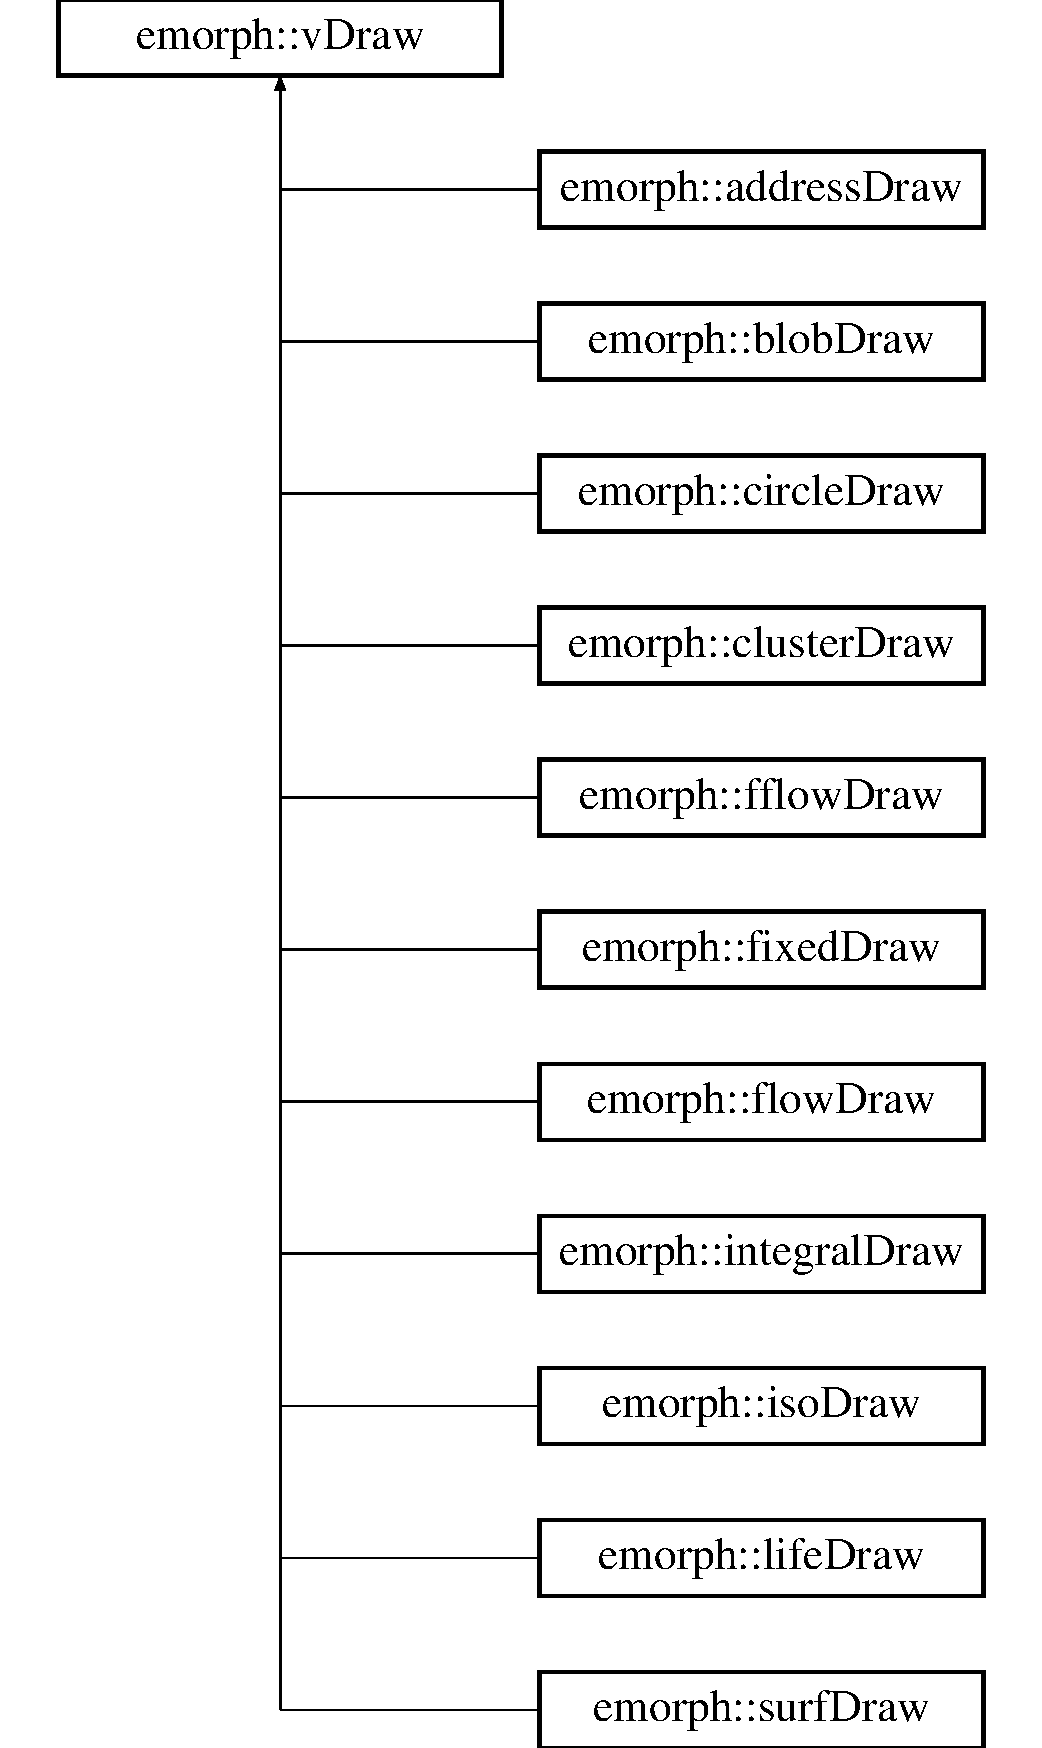
\includegraphics[height=12.000000cm]{classemorph_1_1vDraw}
\end{center}
\end{figure}
\subsection*{Public Member Functions}
\begin{DoxyCompactItemize}
\item 
void \hyperlink{classemorph_1_1vDraw_a2f3fcaac36593cb22d7972a27e0f88fa}{set\-Limits} (int Xlimit, int Ylimit)
\begin{DoxyCompactList}\small\item\em set\-Limits sets the maximum possible values of the position of events that could be drawn (mostly governed by the sensor size). \end{DoxyCompactList}\item 
virtual void \hyperlink{classemorph_1_1vDraw_af10374185b2bd6f6e099325ec5815847}{draw} (cv\-::\-Mat \&canvas, const \hyperlink{classemorph_1_1vQueue}{emorph\-::v\-Queue} \&e\-Set)=0
\begin{DoxyCompactList}\small\item\em draw takes an image and overlays the new visualisation textures \end{DoxyCompactList}\item 
virtual std\-::string \hyperlink{classemorph_1_1vDraw_a3d238b29b58fb63ae3f7d258a199bb68}{get\-Tag} ()=0
\begin{DoxyCompactList}\small\item\em get\-Tag returns the unique code for this drawing method. The arguments given on the command line must match this code exactly \end{DoxyCompactList}\end{DoxyCompactItemize}
\subsection*{Protected Member Functions}
\begin{DoxyCompactItemize}
\item 
\hypertarget{classemorph_1_1vDraw_a2cadf813b464b80ec399a2a80e81451e}{int {\bfseries check\-Stagnancy} (const \hyperlink{classemorph_1_1vQueue}{emorph\-::v\-Queue} \&e\-Set)}\label{classemorph_1_1vDraw_a2cadf813b464b80ec399a2a80e81451e}

\end{DoxyCompactItemize}
\subsection*{Protected Attributes}
\begin{DoxyCompactItemize}
\item 
\hypertarget{classemorph_1_1vDraw_a78bd4c31cc63ee1defafde0827168437}{int {\bfseries Xlimit}}\label{classemorph_1_1vDraw_a78bd4c31cc63ee1defafde0827168437}

\item 
\hypertarget{classemorph_1_1vDraw_a1852c9380bf148cead8a3f0a4c8c593d}{int {\bfseries Ylimit}}\label{classemorph_1_1vDraw_a1852c9380bf148cead8a3f0a4c8c593d}

\item 
\hypertarget{classemorph_1_1vDraw_a1e3b347cd2f7f36026c3dc0b938da6aa}{int {\bfseries stagnant\-Count}}\label{classemorph_1_1vDraw_a1e3b347cd2f7f36026c3dc0b938da6aa}

\item 
\hypertarget{classemorph_1_1vDraw_aed9cc2dfe52cb25e2aa4ff3ffb1cb27a}{int {\bfseries p\-T\-S}}\label{classemorph_1_1vDraw_aed9cc2dfe52cb25e2aa4ff3ffb1cb27a}

\item 
\hypertarget{classemorph_1_1vDraw_a78d59852d20e5ebf88c8152501095f9b}{int {\bfseries clear\-Threshold}}\label{classemorph_1_1vDraw_a78d59852d20e5ebf88c8152501095f9b}

\end{DoxyCompactItemize}


\subsection{Detailed Description}
The \hyperlink{classemorph_1_1vDraw}{v\-Draw} class is the base class from which all v\-Drawers should inherit. It contains the draw and get\-Tag functions which must be overloaded, and the sensor size for reference. 

\subsection{Member Function Documentation}
\hypertarget{classemorph_1_1vDraw_af10374185b2bd6f6e099325ec5815847}{\index{emorph\-::v\-Draw@{emorph\-::v\-Draw}!draw@{draw}}
\index{draw@{draw}!emorph::vDraw@{emorph\-::v\-Draw}}
\subsubsection[{draw}]{\setlength{\rightskip}{0pt plus 5cm}virtual void emorph\-::v\-Draw\-::draw (
\begin{DoxyParamCaption}
\item[{cv\-::\-Mat \&}]{canvas, }
\item[{const {\bf emorph\-::v\-Queue} \&}]{e\-Set}
\end{DoxyParamCaption}
)\hspace{0.3cm}{\ttfamily [pure virtual]}}}\label{classemorph_1_1vDraw_af10374185b2bd6f6e099325ec5815847}


draw takes an image and overlays the new visualisation textures 


\begin{DoxyParams}{Parameters}
{\em canvas} & is the image which may or may not yet exist \\
\hline
{\em e\-Set} & is the set of events which could possibly be drawn \\
\hline
\end{DoxyParams}


Implemented in \hyperlink{classemorph_1_1isoDraw_aa30dd2dbb7d8f9f087f48582b6772d69}{emorph\-::iso\-Draw}, \hyperlink{classemorph_1_1fflowDraw_ae2214e69d31fb9fdcab0e5ba9c8b6f99}{emorph\-::fflow\-Draw}, \hyperlink{classemorph_1_1fixedDraw_a6023c32885fc396258fd111a0ed277c6}{emorph\-::fixed\-Draw}, \hyperlink{classemorph_1_1surfDraw_a3b448daead5d0bbc9e61fdc0022c0c8b}{emorph\-::surf\-Draw}, \hyperlink{classemorph_1_1circleDraw_a03dde28736c280049798d5f9619a8be5}{emorph\-::circle\-Draw}, \hyperlink{classemorph_1_1blobDraw_af2be44e448d04221db47e9b21b03aeec}{emorph\-::blob\-Draw}, \hyperlink{classemorph_1_1clusterDraw_a79e1d35439561ce08431da19a480e88c}{emorph\-::cluster\-Draw}, \hyperlink{classemorph_1_1flowDraw_a28eeaf6490d8e4f5b334200562d2c31b}{emorph\-::flow\-Draw}, \hyperlink{classemorph_1_1integralDraw_a18b3d64b6b81b43c66df4c67955429ff}{emorph\-::integral\-Draw}, \hyperlink{classemorph_1_1lifeDraw_a2323f8371720151079ab6304d1672853}{emorph\-::life\-Draw}, and \hyperlink{classemorph_1_1addressDraw_a31228f7f61455afb4b7b1536e601c854}{emorph\-::address\-Draw}.

\hypertarget{classemorph_1_1vDraw_a3d238b29b58fb63ae3f7d258a199bb68}{\index{emorph\-::v\-Draw@{emorph\-::v\-Draw}!get\-Tag@{get\-Tag}}
\index{get\-Tag@{get\-Tag}!emorph::vDraw@{emorph\-::v\-Draw}}
\subsubsection[{get\-Tag}]{\setlength{\rightskip}{0pt plus 5cm}virtual std\-::string emorph\-::v\-Draw\-::get\-Tag (
\begin{DoxyParamCaption}
{}
\end{DoxyParamCaption}
)\hspace{0.3cm}{\ttfamily [pure virtual]}}}\label{classemorph_1_1vDraw_a3d238b29b58fb63ae3f7d258a199bb68}


get\-Tag returns the unique code for this drawing method. The arguments given on the command line must match this code exactly 

\begin{DoxyReturn}{Returns}
the tag code 
\end{DoxyReturn}


Implemented in \hyperlink{classemorph_1_1isoDraw_a9c62708bc4446b0e55cddb9f47e31d89}{emorph\-::iso\-Draw}, \hyperlink{classemorph_1_1fflowDraw_a742dbd851c4c3a9aca679505571f951d}{emorph\-::fflow\-Draw}, \hyperlink{classemorph_1_1fixedDraw_a3b703843af2824a63c27aacb713d7f50}{emorph\-::fixed\-Draw}, \hyperlink{classemorph_1_1surfDraw_aa65dc027fd2d96a01218230525f270e2}{emorph\-::surf\-Draw}, \hyperlink{classemorph_1_1circleDraw_ae725bd75bc70f72c14c1d01e0365080b}{emorph\-::circle\-Draw}, \hyperlink{classemorph_1_1blobDraw_ad0970eb3689b4fb08aec786184ec2f92}{emorph\-::blob\-Draw}, \hyperlink{classemorph_1_1clusterDraw_a2b6aff21bcfc2088f8b580ee8a0e74ba}{emorph\-::cluster\-Draw}, \hyperlink{classemorph_1_1flowDraw_a3ba90985c688de6ac753b575e7a322f0}{emorph\-::flow\-Draw}, \hyperlink{classemorph_1_1integralDraw_a3383c3587a1d99fb3a2352ae4e02371d}{emorph\-::integral\-Draw}, \hyperlink{classemorph_1_1lifeDraw_a11b718fa894541473ea67e0d98331d7a}{emorph\-::life\-Draw}, and \hyperlink{classemorph_1_1addressDraw_a82a6050de6d2950cb6598b0f64cada24}{emorph\-::address\-Draw}.

\hypertarget{classemorph_1_1vDraw_a2f3fcaac36593cb22d7972a27e0f88fa}{\index{emorph\-::v\-Draw@{emorph\-::v\-Draw}!set\-Limits@{set\-Limits}}
\index{set\-Limits@{set\-Limits}!emorph::vDraw@{emorph\-::v\-Draw}}
\subsubsection[{set\-Limits}]{\setlength{\rightskip}{0pt plus 5cm}void emorph\-::v\-Draw\-::set\-Limits (
\begin{DoxyParamCaption}
\item[{int}]{Xlimit, }
\item[{int}]{Ylimit}
\end{DoxyParamCaption}
)\hspace{0.3cm}{\ttfamily [inline]}}}\label{classemorph_1_1vDraw_a2f3fcaac36593cb22d7972a27e0f88fa}


set\-Limits sets the maximum possible values of the position of events that could be drawn (mostly governed by the sensor size). 


\begin{DoxyParams}{Parameters}
{\em Xlimit} & is the maximum x value (width) \\
\hline
{\em Ylimit} & is the maximium y value (height) \\
\hline
\end{DoxyParams}


The documentation for this class was generated from the following file\-:\begin{DoxyCompactItemize}
\item 
/home/aglover/workspace/projects/event\-Driven/src/visualization/v\-Framer/include/i\-Cub/v\-Draw.\-h\end{DoxyCompactItemize}

\hypertarget{classemorph_1_1vEvent}{\section{emorph\-:\-:v\-Event Class Reference}
\label{classemorph_1_1vEvent}\index{emorph\-::v\-Event@{emorph\-::v\-Event}}
}
Inheritance diagram for emorph\-:\-:v\-Event\-:\begin{figure}[H]
\begin{center}
\leavevmode
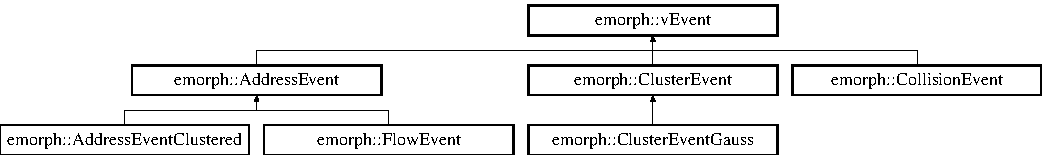
\includegraphics[height=2.089552cm]{classemorph_1_1vEvent}
\end{center}
\end{figure}
\subsection*{Public Member Functions}
\begin{DoxyCompactItemize}
\item 
\hypertarget{classemorph_1_1vEvent_ac5c3b0192528acbf4e68805e461fd734}{\hyperlink{classemorph_1_1vEvent_ac5c3b0192528acbf4e68805e461fd734}{v\-Event} ()}\label{classemorph_1_1vEvent_ac5c3b0192528acbf4e68805e461fd734}

\begin{DoxyCompactList}\small\item\em blank constructor required at base level \end{DoxyCompactList}\item 
\hypertarget{classemorph_1_1vEvent_af2f61582ba903b46ec530d8a9df49453}{\hyperlink{classemorph_1_1vEvent_af2f61582ba903b46ec530d8a9df49453}{v\-Event} (const \hyperlink{classemorph_1_1vEvent}{v\-Event} \&event)}\label{classemorph_1_1vEvent_af2f61582ba903b46ec530d8a9df49453}

\begin{DoxyCompactList}\small\item\em copy constructor \end{DoxyCompactList}\item 
\hypertarget{classemorph_1_1vEvent_a827ccbd7bf7ddd10923dfaf2aac1a0b4}{void {\bfseries referto} ()}\label{classemorph_1_1vEvent_a827ccbd7bf7ddd10923dfaf2aac1a0b4}

\item 
\hypertarget{classemorph_1_1vEvent_abda4cc0ab6fd16abd9f5da13145ab967}{void {\bfseries destroy} ()}\label{classemorph_1_1vEvent_abda4cc0ab6fd16abd9f5da13145ab967}

\item 
\hypertarget{classemorph_1_1vEvent_ae99765d28e2628d92fe4985d5a4e7951}{virtual std\-::string {\bfseries get\-Type} () const }\label{classemorph_1_1vEvent_ae99765d28e2628d92fe4985d5a4e7951}

\item 
\hypertarget{classemorph_1_1vEvent_ab17df1991d168aa8aa43eddd57dc6e04}{void {\bfseries set\-Stamp} (const long int stamp)}\label{classemorph_1_1vEvent_ab17df1991d168aa8aa43eddd57dc6e04}

\item 
\hypertarget{classemorph_1_1vEvent_a2fe87097119e68760bd4bfe9511e1c54}{int {\bfseries get\-Stamp} () const }\label{classemorph_1_1vEvent_a2fe87097119e68760bd4bfe9511e1c54}

\item 
\hypertarget{classemorph_1_1vEvent_a8cb587b03ff0432d8665ff8a2c2d517c}{virtual int {\bfseries get\-Channel} () const }\label{classemorph_1_1vEvent_a8cb587b03ff0432d8665ff8a2c2d517c}

\item 
\hypertarget{classemorph_1_1vEvent_a694ba5711b4bbf8bfd8743b60006d53f}{virtual int {\bfseries get\-Polarity} () const }\label{classemorph_1_1vEvent_a694ba5711b4bbf8bfd8743b60006d53f}

\item 
\hypertarget{classemorph_1_1vEvent_a9e5dea4caa64e1dedece71339be427ac}{virtual \hyperlink{classemorph_1_1vEvent}{v\-Event} \& {\bfseries operator=} (const \hyperlink{classemorph_1_1vEvent}{v\-Event} \&event)}\label{classemorph_1_1vEvent_a9e5dea4caa64e1dedece71339be427ac}

\item 
\hypertarget{classemorph_1_1vEvent_a48e0878410a8da3449220fe7f337a159}{virtual bool {\bfseries operator==} (const \hyperlink{classemorph_1_1vEvent}{v\-Event} \&event)}\label{classemorph_1_1vEvent_a48e0878410a8da3449220fe7f337a159}

\item 
\hypertarget{classemorph_1_1vEvent_af2901f070adea52495d9b0414ed90e95}{virtual bool {\bfseries operator$<$} (const \hyperlink{classemorph_1_1vEvent}{v\-Event} \&event) const }\label{classemorph_1_1vEvent_af2901f070adea52495d9b0414ed90e95}

\item 
\hypertarget{classemorph_1_1vEvent_a8a55fc59b331f93cb95829dee21ef3dc}{virtual bool {\bfseries operator$>$} (const \hyperlink{classemorph_1_1vEvent}{v\-Event} \&event) const }\label{classemorph_1_1vEvent_a8a55fc59b331f93cb95829dee21ef3dc}

\item 
\hypertarget{classemorph_1_1vEvent_a73d24674b7e5ece51cda67f4e10bd312}{virtual \hyperlink{classemorph_1_1vEvent}{v\-Event} $\ast$ {\bfseries clone} ()}\label{classemorph_1_1vEvent_a73d24674b7e5ece51cda67f4e10bd312}

\item 
\hypertarget{classemorph_1_1vEvent_ae2eb881db166370eac07f9e4bcd22cdf}{virtual void {\bfseries encode} (yarp\-::os\-::\-Bottle \&b) const }\label{classemorph_1_1vEvent_ae2eb881db166370eac07f9e4bcd22cdf}

\item 
\hypertarget{classemorph_1_1vEvent_a75b5c46b819fc8693749e4eb0ab3e91f}{virtual bool {\bfseries decode} (const yarp\-::os\-::\-Bottle \&packet, int \&pos)}\label{classemorph_1_1vEvent_a75b5c46b819fc8693749e4eb0ab3e91f}

\item 
\hypertarget{classemorph_1_1vEvent_a54209948752ced6d6ed0c6a5612dd42b}{virtual yarp\-::os\-::\-Property {\bfseries get\-Content} () const }\label{classemorph_1_1vEvent_a54209948752ced6d6ed0c6a5612dd42b}

\item 
\hypertarget{classemorph_1_1vEvent_a851e06124d640e2f43ef99049a587607}{virtual int {\bfseries n\-Bytes\-Coded} () const }\label{classemorph_1_1vEvent_a851e06124d640e2f43ef99049a587607}

\item 
\hypertarget{classemorph_1_1vEvent_a7a4ea1e06c31602ae08d85e974b24aba}{{\footnotesize template$<$class T $>$ }\\T $\ast$ {\bfseries get\-As} ()}\label{classemorph_1_1vEvent_a7a4ea1e06c31602ae08d85e974b24aba}

\item 
\hypertarget{classemorph_1_1vEvent_affe99b3696590fd050d8912d88006d43}{{\footnotesize template$<$class T $>$ }\\T $\ast$ {\bfseries get\-Unsafe} ()}\label{classemorph_1_1vEvent_affe99b3696590fd050d8912d88006d43}

\end{DoxyCompactItemize}
\subsection*{Public Attributes}
\begin{DoxyCompactItemize}
\item 
\hypertarget{classemorph_1_1vEvent_ac92466be7aee7e911a4fd2d578bfe90b}{int {\bfseries refcount}}\label{classemorph_1_1vEvent_ac92466be7aee7e911a4fd2d578bfe90b}

\end{DoxyCompactItemize}
\subsection*{Protected Attributes}
\begin{DoxyCompactItemize}
\item 
\hypertarget{classemorph_1_1vEvent_aba25704ab1a865d995734bba01813778}{int {\bfseries stamp}}\label{classemorph_1_1vEvent_aba25704ab1a865d995734bba01813778}

\end{DoxyCompactItemize}
\subsection*{Static Protected Attributes}
\begin{DoxyCompactItemize}
\item 
\hypertarget{classemorph_1_1vEvent_aee7f41632af3f665d74a90d89a16dfbc}{static const unsigned int {\bfseries max\-\_\-stamp} = 16777215}\label{classemorph_1_1vEvent_aee7f41632af3f665d74a90d89a16dfbc}

\end{DoxyCompactItemize}


The documentation for this class was generated from the following files\-:\begin{DoxyCompactItemize}
\item 
/home/aglover/workspace/projects/event\-Driven/emorph\-\_\-lib/include/i\-Cub/emorph/v\-Codec.\-h\item 
/home/aglover/workspace/projects/event\-Driven/emorph\-\_\-lib/src/v\-Codec.\-cpp\end{DoxyCompactItemize}

\hypertarget{classvFlowManager}{\section{v\-Flow\-Manager Class Reference}
\label{classvFlowManager}\index{v\-Flow\-Manager@{v\-Flow\-Manager}}
}


The \hyperlink{classvFlowManager}{v\-Flow\-Manager} class performs event-\/based optical flow.  




{\ttfamily \#include $<$v\-Flow.\-h$>$}

Inheritance diagram for v\-Flow\-Manager\-:\begin{figure}[H]
\begin{center}
\leavevmode
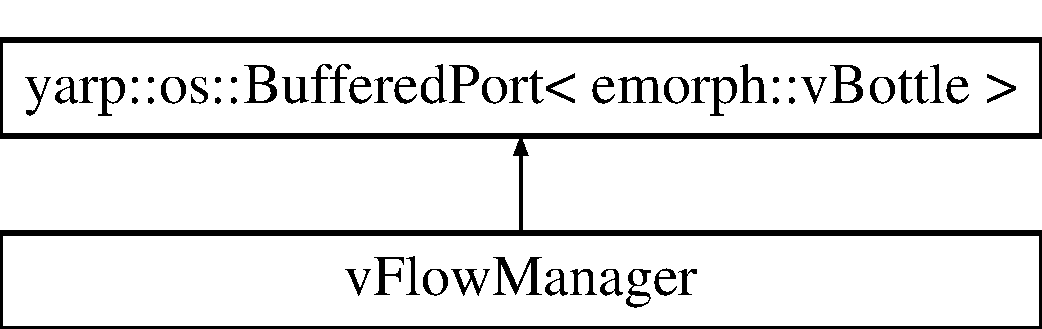
\includegraphics[height=2.000000cm]{classvFlowManager}
\end{center}
\end{figure}
\subsection*{Public Member Functions}
\begin{DoxyCompactItemize}
\item 
\hypertarget{classvFlowManager_a9d28c98ce6f6c0591a89f5055153e295}{{\bfseries v\-Flow\-Manager} (int height, int width, int filter\-Size, int min\-Evts\-On\-Plane)}\label{classvFlowManager_a9d28c98ce6f6c0591a89f5055153e295}

\item 
bool \hyperlink{classvFlowManager_a2c299db37662565d5b0c59679b790a4b}{open} (std\-::string module\-Name, bool strictness=false)
\begin{DoxyCompactList}\small\item\em open the port and start callback \end{DoxyCompactList}\item 
\hypertarget{classvFlowManager_abcf434ef8391ec6741c0754bc4a88ab8}{void {\bfseries close} ()}\label{classvFlowManager_abcf434ef8391ec6741c0754bc4a88ab8}

\item 
\hypertarget{classvFlowManager_a10d85ce69f60a672adba81aff4a046d8}{void {\bfseries interrupt} ()}\label{classvFlowManager_a10d85ce69f60a672adba81aff4a046d8}

\item 
\hypertarget{classvFlowManager_a67113d949355705533cc65aca8a15b40}{void {\bfseries on\-Read} (\hyperlink{classemorph_1_1vBottle}{emorph\-::v\-Bottle} \&in\-Bottle)}\label{classvFlowManager_a67113d949355705533cc65aca8a15b40}

\end{DoxyCompactItemize}


\subsection{Detailed Description}
The \hyperlink{classvFlowManager}{v\-Flow\-Manager} class performs event-\/based optical flow. 

\subsection{Member Function Documentation}
\hypertarget{classvFlowManager_a2c299db37662565d5b0c59679b790a4b}{\index{v\-Flow\-Manager@{v\-Flow\-Manager}!open@{open}}
\index{open@{open}!vFlowManager@{v\-Flow\-Manager}}
\subsubsection[{open}]{\setlength{\rightskip}{0pt plus 5cm}bool v\-Flow\-Manager\-::open (
\begin{DoxyParamCaption}
\item[{std\-::string}]{module\-Name, }
\item[{bool}]{strictness = {\ttfamily false}}
\end{DoxyParamCaption}
)}}\label{classvFlowManager_a2c299db37662565d5b0c59679b790a4b}


open the port and start callback 


\begin{DoxyParams}{Parameters}
{\em module\-Name} & defines port names (default v\-Flow) \\
\hline
{\em strictness} & read and write strcitly such that events are not lost \\
\hline
\end{DoxyParams}
\begin{DoxyReturn}{Returns}
true on successful open 
\end{DoxyReturn}


The documentation for this class was generated from the following files\-:\begin{DoxyCompactItemize}
\item 
/home/aglover/workspace/projects/event\-Driven/src/processing/v\-Flow/include/\hyperlink{vFlow_8h}{v\-Flow.\-h}\item 
/home/aglover/workspace/projects/event\-Driven/src/processing/v\-Flow/src/v\-Flow.\-cpp\end{DoxyCompactItemize}

\hypertarget{classvFlowModule}{\section{v\-Flow\-Module Class Reference}
\label{classvFlowModule}\index{v\-Flow\-Module@{v\-Flow\-Module}}
}
Inheritance diagram for v\-Flow\-Module\-:\begin{figure}[H]
\begin{center}
\leavevmode
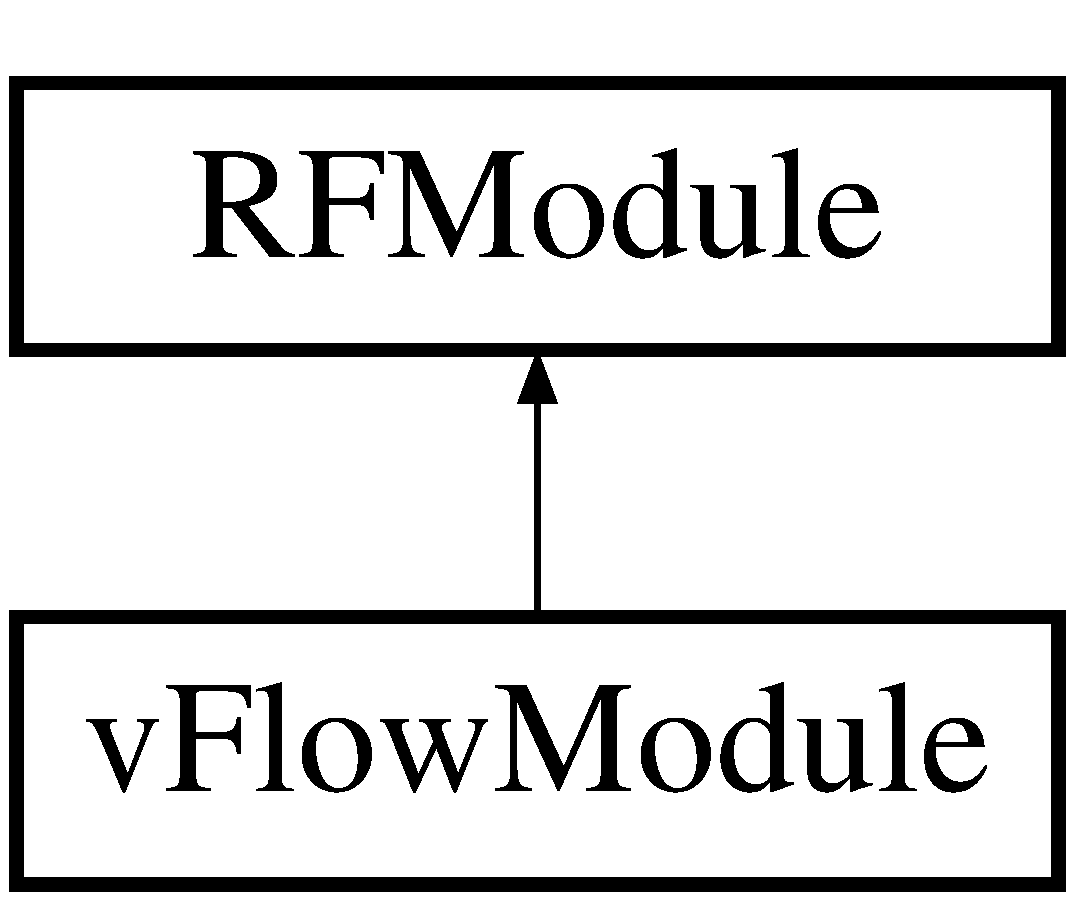
\includegraphics[height=2.000000cm]{classvFlowModule}
\end{center}
\end{figure}
\subsection*{Public Member Functions}
\begin{DoxyCompactItemize}
\item 
\hypertarget{classvFlowModule_a5cf91bc0de9e311b1946c6ec044fd947}{virtual bool {\bfseries configure} (yarp\-::os\-::\-Resource\-Finder \&rf)}\label{classvFlowModule_a5cf91bc0de9e311b1946c6ec044fd947}

\item 
\hypertarget{classvFlowModule_a49a90a2d595d99bf290423dd930eefe2}{virtual bool {\bfseries interrupt\-Module} ()}\label{classvFlowModule_a49a90a2d595d99bf290423dd930eefe2}

\item 
\hypertarget{classvFlowModule_a63a3da2ac7ba9631753ea244d8bc4358}{virtual bool {\bfseries close} ()}\label{classvFlowModule_a63a3da2ac7ba9631753ea244d8bc4358}

\item 
\hypertarget{classvFlowModule_a880de21f5c85d684f7c0999d0a84e26b}{virtual bool {\bfseries update\-Module} ()}\label{classvFlowModule_a880de21f5c85d684f7c0999d0a84e26b}

\item 
\hypertarget{classvFlowModule_a8f6f74c4a7888e162c2dff8a34a84323}{virtual double {\bfseries get\-Period} ()}\label{classvFlowModule_a8f6f74c4a7888e162c2dff8a34a84323}

\end{DoxyCompactItemize}


The documentation for this class was generated from the following files\-:\begin{DoxyCompactItemize}
\item 
/home/aglover/workspace/projects/event\-Driven/src/processing/v\-Flow/include/\hyperlink{vFlow_8h}{v\-Flow.\-h}\item 
/home/aglover/workspace/projects/event\-Driven/src/processing/v\-Flow/src/v\-Flow.\-cpp\end{DoxyCompactItemize}

\hypertarget{classemorph_1_1vFramerModule}{\section{emorph\-:\-:v\-Framer\-Module Class Reference}
\label{classemorph_1_1vFramerModule}\index{emorph\-::v\-Framer\-Module@{emorph\-::v\-Framer\-Module}}
}


The \hyperlink{classemorph_1_1vFramerModule}{v\-Framer\-Module} class runs the event reading and channel splitting, the drawing modules, and the yarp image output buffers. Images are created at a rate equal to the rate of this thread.  




{\ttfamily \#include $<$v\-Framer.\-h$>$}

Inheritance diagram for emorph\-:\-:v\-Framer\-Module\-:\begin{figure}[H]
\begin{center}
\leavevmode
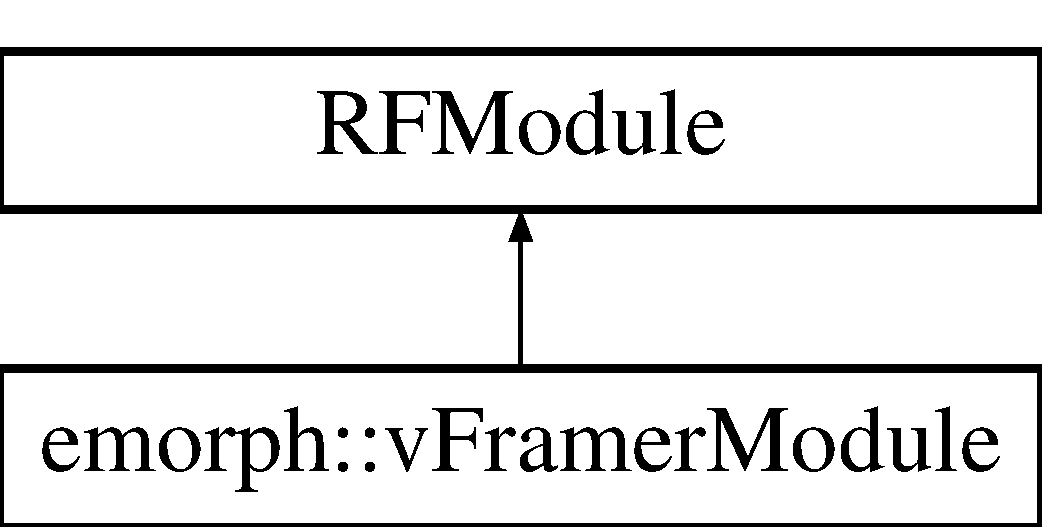
\includegraphics[height=2.000000cm]{classemorph_1_1vFramerModule}
\end{center}
\end{figure}
\subsection*{Public Member Functions}
\begin{DoxyCompactItemize}
\item 
\hypertarget{classemorph_1_1vFramerModule_a0774b49c29a6bf00c3a269573c1e8bb0}{virtual bool {\bfseries configure} (yarp\-::os\-::\-Resource\-Finder \&rf)}\label{classemorph_1_1vFramerModule_a0774b49c29a6bf00c3a269573c1e8bb0}

\item 
\hypertarget{classemorph_1_1vFramerModule_a9718c0d118f0603c131e9033298fa303}{virtual bool {\bfseries interrupt\-Module} ()}\label{classemorph_1_1vFramerModule_a9718c0d118f0603c131e9033298fa303}

\item 
\hypertarget{classemorph_1_1vFramerModule_a6e106a5b6b4bd41fbf3d68ea9a8069b1}{virtual bool {\bfseries close} ()}\label{classemorph_1_1vFramerModule_a6e106a5b6b4bd41fbf3d68ea9a8069b1}

\item 
\hypertarget{classemorph_1_1vFramerModule_a143d9b10c0450a1e1fdd2be472f3c651}{virtual bool {\bfseries respond} (const yarp\-::os\-::\-Bottle \&command, yarp\-::os\-::\-Bottle \&reply)}\label{classemorph_1_1vFramerModule_a143d9b10c0450a1e1fdd2be472f3c651}

\item 
\hypertarget{classemorph_1_1vFramerModule_aa6d5d465684f59f9eada49e8b8abae59}{virtual bool {\bfseries update\-Module} ()}\label{classemorph_1_1vFramerModule_aa6d5d465684f59f9eada49e8b8abae59}

\item 
\hypertarget{classemorph_1_1vFramerModule_a91b423c2b14eb2ad9f4bb5e25dbfd01b}{virtual double {\bfseries get\-Period} ()}\label{classemorph_1_1vFramerModule_a91b423c2b14eb2ad9f4bb5e25dbfd01b}

\end{DoxyCompactItemize}


\subsection{Detailed Description}
The \hyperlink{classemorph_1_1vFramerModule}{v\-Framer\-Module} class runs the event reading and channel splitting, the drawing modules, and the yarp image output buffers. Images are created at a rate equal to the rate of this thread. 

The documentation for this class was generated from the following files\-:\begin{DoxyCompactItemize}
\item 
/home/aglover/workspace/projects/event\-Driven/src/visualization/v\-Framer/include/i\-Cub/v\-Framer.\-h\item 
/home/aglover/workspace/projects/event\-Driven/src/visualization/v\-Framer/src/v\-Framer.\-cpp\end{DoxyCompactItemize}

\hypertarget{classemorph_1_1vQueue}{\section{emorph\-:\-:v\-Queue Class Reference}
\label{classemorph_1_1vQueue}\index{emorph\-::v\-Queue@{emorph\-::v\-Queue}}
}
Inheritance diagram for emorph\-:\-:v\-Queue\-:\begin{figure}[H]
\begin{center}
\leavevmode
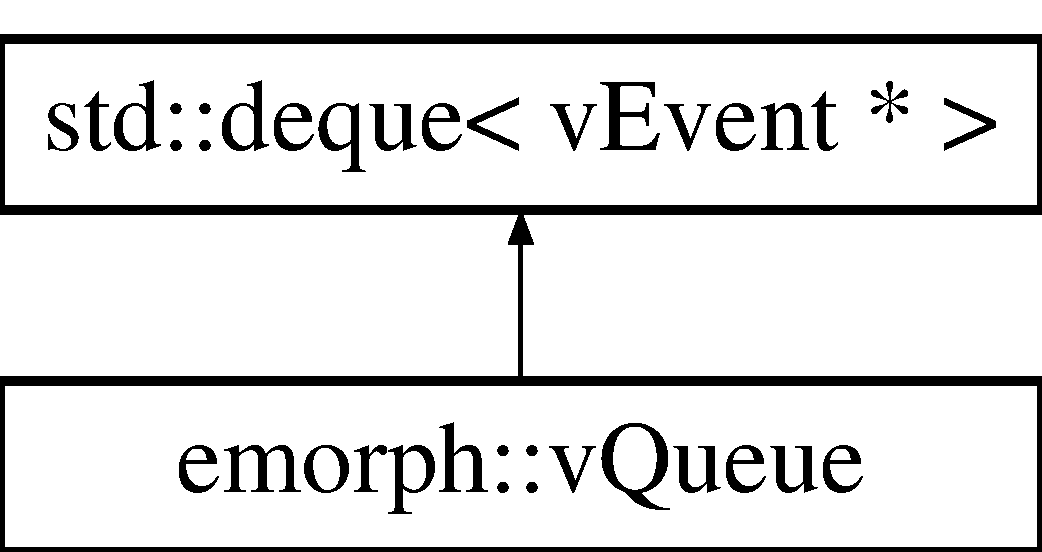
\includegraphics[height=2.000000cm]{classemorph_1_1vQueue}
\end{center}
\end{figure}
\subsection*{Public Member Functions}
\begin{DoxyCompactItemize}
\item 
\hypertarget{classemorph_1_1vQueue_a8fc30b31447daf707b487c59c3474422}{virtual void {\bfseries clear} ()}\label{classemorph_1_1vQueue_a8fc30b31447daf707b487c59c3474422}

\item 
\hypertarget{classemorph_1_1vQueue_ab712a257395e442920ac0ca155080821}{{\bfseries v\-Queue} (const \hyperlink{classemorph_1_1vQueue}{v\-Queue} \&)}\label{classemorph_1_1vQueue_ab712a257395e442920ac0ca155080821}

\item 
\hypertarget{classemorph_1_1vQueue_acdd95854b75e08d82acc830de06c2377}{\hyperlink{classemorph_1_1vQueue}{v\-Queue} \& {\bfseries operator=} (const \hyperlink{classemorph_1_1vQueue}{v\-Queue} \&)}\label{classemorph_1_1vQueue_acdd95854b75e08d82acc830de06c2377}

\item 
\hypertarget{classemorph_1_1vQueue_a81fb5370e1ea9351a61225e86427651c}{virtual void {\bfseries push\-\_\-back} (const value\-\_\-type \&\-\_\-\-\_\-x)}\label{classemorph_1_1vQueue_a81fb5370e1ea9351a61225e86427651c}

\item 
\hypertarget{classemorph_1_1vQueue_a1d288086d56b6e03f39ce85210430ff0}{virtual void {\bfseries push\-\_\-front} (const value\-\_\-type \&\-\_\-\-\_\-x)}\label{classemorph_1_1vQueue_a1d288086d56b6e03f39ce85210430ff0}

\item 
\hypertarget{classemorph_1_1vQueue_a269240a67fd853ad94ebc11a0aac1f59}{virtual void {\bfseries pop\-\_\-back} ()}\label{classemorph_1_1vQueue_a269240a67fd853ad94ebc11a0aac1f59}

\item 
\hypertarget{classemorph_1_1vQueue_a4d66963ef50b8b518955ac2f744cf47f}{virtual void {\bfseries pop\-\_\-front} ()}\label{classemorph_1_1vQueue_a4d66963ef50b8b518955ac2f744cf47f}

\item 
\hypertarget{classemorph_1_1vQueue_ab79af1dcb8978f327e72ba5832dad67f}{virtual iterator {\bfseries erase} (iterator \-\_\-\-\_\-first, iterator \-\_\-\-\_\-last)}\label{classemorph_1_1vQueue_ab79af1dcb8978f327e72ba5832dad67f}

\item 
\hypertarget{classemorph_1_1vQueue_ac8f2ae2f4c240a774ebfc31bea860817}{virtual iterator {\bfseries erase} (iterator \-\_\-\-\_\-position)}\label{classemorph_1_1vQueue_ac8f2ae2f4c240a774ebfc31bea860817}

\item 
\hypertarget{classemorph_1_1vQueue_abe1401ff2ff49bf3aa53c50ee9444c3e}{void {\bfseries sort} ()}\label{classemorph_1_1vQueue_abe1401ff2ff49bf3aa53c50ee9444c3e}

\item 
\hypertarget{classemorph_1_1vQueue_a995f8d91ead68c307b7d1ab706e03f2b}{void {\bfseries wrap\-Sort} ()}\label{classemorph_1_1vQueue_a995f8d91ead68c307b7d1ab706e03f2b}

\end{DoxyCompactItemize}


The documentation for this class was generated from the following files\-:\begin{DoxyCompactItemize}
\item 
/home/aglover/workspace/projects/event\-Driven/emorph\-\_\-lib/include/i\-Cub/emorph/v\-Queue.\-h\item 
/home/aglover/workspace/projects/event\-Driven/emorph\-\_\-lib/src/v\-Queue.\-cpp\end{DoxyCompactItemize}

\hypertarget{classemorph_1_1vReadAndSplit}{\section{emorph\-:\-:v\-Read\-And\-Split Class Reference}
\label{classemorph_1_1vReadAndSplit}\index{emorph\-::v\-Read\-And\-Split@{emorph\-::v\-Read\-And\-Split}}
}


The \hyperlink{classemorph_1_1vReadAndSplit}{v\-Read\-And\-Split} class splits events into different v\-Windows based on the channel parameter. At any point in time a snapshot of all windows can be performed, after which the resulting v\-Queues can be accessed.  




{\ttfamily \#include $<$v\-Framer.\-h$>$}

Inheritance diagram for emorph\-:\-:v\-Read\-And\-Split\-:\begin{figure}[H]
\begin{center}
\leavevmode
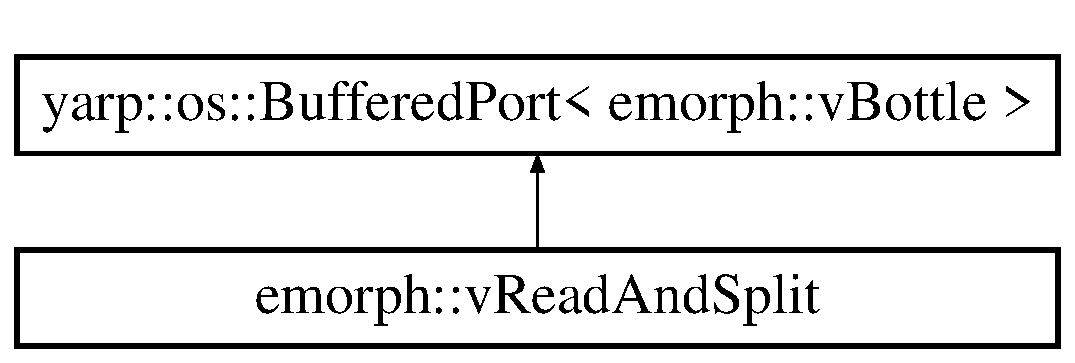
\includegraphics[height=2.000000cm]{classemorph_1_1vReadAndSplit}
\end{center}
\end{figure}
\subsection*{Public Member Functions}
\begin{DoxyCompactItemize}
\item 
\hypertarget{classemorph_1_1vReadAndSplit_a58ed7a0a18a7c11a5d997c8deec0bd3d}{\hyperlink{classemorph_1_1vReadAndSplit_a58ed7a0a18a7c11a5d997c8deec0bd3d}{v\-Read\-And\-Split} ()}\label{classemorph_1_1vReadAndSplit_a58ed7a0a18a7c11a5d997c8deec0bd3d}

\begin{DoxyCompactList}\small\item\em \hyperlink{classemorph_1_1vReadAndSplit}{v\-Read\-And\-Split} constructor with default windowsize parameter \end{DoxyCompactList}\item 
void \hyperlink{classemorph_1_1vReadAndSplit_ab59e77834ba842a6508b174c48b5cda2}{set\-Window\-Size} (int windowsize)
\begin{DoxyCompactList}\small\item\em set\-Window\-Size sets the length of time events are stored \end{DoxyCompactList}\item 
\hypertarget{classemorph_1_1vReadAndSplit_a39e2a1c330b7b2bde69544183219a0fa}{void \hyperlink{classemorph_1_1vReadAndSplit_a39e2a1c330b7b2bde69544183219a0fa}{snapshot\-All\-Windows} ()}\label{classemorph_1_1vReadAndSplit_a39e2a1c330b7b2bde69544183219a0fa}

\begin{DoxyCompactList}\small\item\em snapshot\-All\-Windows freeze the current list of events for each channel \end{DoxyCompactList}\item 
const \hyperlink{classemorph_1_1vQueue}{emorph\-::v\-Queue} \& \hyperlink{classemorph_1_1vReadAndSplit_a47fa3402c835dfb703090cce063d472f}{get\-Snap} (const int channel)
\begin{DoxyCompactList}\small\item\em get\-Snap get a list of snapshotted events \end{DoxyCompactList}\item 
virtual void \hyperlink{classemorph_1_1vReadAndSplit_a1d8534ca9c14f84159546d9d2fb6fd75}{on\-Read} (\hyperlink{classemorph_1_1vBottle}{emorph\-::v\-Bottle} \&incoming)
\begin{DoxyCompactList}\small\item\em on\-Read splitting is performed as an asynchronous on\-Read function \end{DoxyCompactList}\item 
\hypertarget{classemorph_1_1vReadAndSplit_a1896b51ae1e8c9d13d875d37c2319b97}{virtual bool {\bfseries open} (const std\-::string port\-Name)}\label{classemorph_1_1vReadAndSplit_a1896b51ae1e8c9d13d875d37c2319b97}

\end{DoxyCompactItemize}


\subsection{Detailed Description}
The \hyperlink{classemorph_1_1vReadAndSplit}{v\-Read\-And\-Split} class splits events into different v\-Windows based on the channel parameter. At any point in time a snapshot of all windows can be performed, after which the resulting v\-Queues can be accessed. 

\subsection{Member Function Documentation}
\hypertarget{classemorph_1_1vReadAndSplit_a47fa3402c835dfb703090cce063d472f}{\index{emorph\-::v\-Read\-And\-Split@{emorph\-::v\-Read\-And\-Split}!get\-Snap@{get\-Snap}}
\index{get\-Snap@{get\-Snap}!emorph::vReadAndSplit@{emorph\-::v\-Read\-And\-Split}}
\subsubsection[{get\-Snap}]{\setlength{\rightskip}{0pt plus 5cm}const {\bf emorph\-::v\-Queue} \& emorph\-::v\-Read\-And\-Split\-::get\-Snap (
\begin{DoxyParamCaption}
\item[{const int}]{channel}
\end{DoxyParamCaption}
)}}\label{classemorph_1_1vReadAndSplit_a47fa3402c835dfb703090cce063d472f}


get\-Snap get a list of snapshotted events 


\begin{DoxyParams}{Parameters}
{\em channel} & the channel value to access \\
\hline
\end{DoxyParams}
\begin{DoxyReturn}{Returns}
the list of events in a \hyperlink{classemorph_1_1vQueue}{v\-Queue} 
\end{DoxyReturn}
\hypertarget{classemorph_1_1vReadAndSplit_a1d8534ca9c14f84159546d9d2fb6fd75}{\index{emorph\-::v\-Read\-And\-Split@{emorph\-::v\-Read\-And\-Split}!on\-Read@{on\-Read}}
\index{on\-Read@{on\-Read}!emorph::vReadAndSplit@{emorph\-::v\-Read\-And\-Split}}
\subsubsection[{on\-Read}]{\setlength{\rightskip}{0pt plus 5cm}void emorph\-::v\-Read\-And\-Split\-::on\-Read (
\begin{DoxyParamCaption}
\item[{{\bf emorph\-::v\-Bottle} \&}]{incoming}
\end{DoxyParamCaption}
)\hspace{0.3cm}{\ttfamily [virtual]}}}\label{classemorph_1_1vReadAndSplit_a1d8534ca9c14f84159546d9d2fb6fd75}


on\-Read splitting is performed as an asynchronous on\-Read function 


\begin{DoxyParams}{Parameters}
{\em incoming} & the \hyperlink{classemorph_1_1vBottle}{v\-Bottle} with events of all channels \\
\hline
\end{DoxyParams}
\hypertarget{classemorph_1_1vReadAndSplit_ab59e77834ba842a6508b174c48b5cda2}{\index{emorph\-::v\-Read\-And\-Split@{emorph\-::v\-Read\-And\-Split}!set\-Window\-Size@{set\-Window\-Size}}
\index{set\-Window\-Size@{set\-Window\-Size}!emorph::vReadAndSplit@{emorph\-::v\-Read\-And\-Split}}
\subsubsection[{set\-Window\-Size}]{\setlength{\rightskip}{0pt plus 5cm}void emorph\-::v\-Read\-And\-Split\-::set\-Window\-Size (
\begin{DoxyParamCaption}
\item[{int}]{windowsize}
\end{DoxyParamCaption}
)}}\label{classemorph_1_1vReadAndSplit_ab59e77834ba842a6508b174c48b5cda2}


set\-Window\-Size sets the length of time events are stored 


\begin{DoxyParams}{Parameters}
{\em windowsize} & (in us) \\
\hline
\end{DoxyParams}


The documentation for this class was generated from the following files\-:\begin{DoxyCompactItemize}
\item 
/home/aglover/workspace/projects/event\-Driven/src/visualization/v\-Framer/include/i\-Cub/v\-Framer.\-h\item 
/home/aglover/workspace/projects/event\-Driven/src/visualization/v\-Framer/src/v\-Framer.\-cpp\end{DoxyCompactItemize}

\hypertarget{unionvsctrl__ioctl__arg__t}{\section{vsctrl\-\_\-ioctl\-\_\-arg\-\_\-t Union Reference}
\label{unionvsctrl__ioctl__arg__t}\index{vsctrl\-\_\-ioctl\-\_\-arg\-\_\-t@{vsctrl\-\_\-ioctl\-\_\-arg\-\_\-t}}
}
\subsection*{Public Attributes}
\begin{DoxyCompactItemize}
\item 
\hypertarget{unionvsctrl__ioctl__arg__t_a964ccf1f18660451105f3f4d11f3b350}{\begin{tabbing}
xx\=xx\=xx\=xx\=xx\=xx\=xx\=xx\=xx\=\kill
struct \{\\
\hypertarget{structvsctrl__ioctl__arg__t_1_1@0_acca01b2b83df159bd627baedbcae7088}{\>uint8\_t {\bfseries addr}\\
\hypertarget{structvsctrl__ioctl__arg__t_1_1@0_a830f110327c3019b4605d9fdf431ba2b}{\>char {\bfseries rw}\\
\hypertarget{structvsctrl__ioctl__arg__t_1_1@0_a32e4d0eda06a0f39312403cb4a38a522}{\>uint32\_t {\bfseries data}\\
\} {\bfseries regs}}\label{unionvsctrl__ioctl__arg__t_a964ccf1f18660451105f3f4d11f3b350}
\\

\end{tabbing}\item 
\hypertarget{unionvsctrl__ioctl__arg__t_a216ca18ed652e07b53e2b62ab1f15c62}{\begin{tabbing}
xx\=xx\=xx\=xx\=xx\=xx\=xx\=xx\=xx\=\kill
struct \{\\
\hypertarget{structvsctrl__ioctl__arg__t_1_1@1_a65ff1a40830e9dfc9a1aa152b7ff7921}{\>uint32\_t {\bfseries prescaler\_value}\\
\hypertarget{structvsctrl__ioctl__arg__t_1_1@1_ac8836d90d5ceb208f0ec55b2ad5e5711}{\>uint8\_t {\bfseries setup\_hold\_time}\\
\hypertarget{structvsctrl__ioctl__arg__t_1_1@1_aaa1204f9bca9864852e0f939b37e2fac}{\>uint8\_t {\bfseries clock\_active\_time}\\
\hypertarget{structvsctrl__ioctl__arg__t_1_1@1_ac47478b97045c4b2901fddd773ef5861}{\>uint8\_t {\bfseries latch\_setup\_time}\\
\hypertarget{structvsctrl__ioctl__arg__t_1_1@1_a480b1ee0443a490f859746d18b448529}{\>uint8\_t {\bfseries latch\_active\_time}\\
\} {\bfseries bg\_timings}}\label{unionvsctrl__ioctl__arg__t_a216ca18ed652e07b53e2b62ab1f15c62}
\\

\end{tabbing}\item 
\hypertarget{unionvsctrl__ioctl__arg__t_a302e104780b085e72586c05f97652b5b}{\begin{tabbing}
xx\=xx\=xx\=xx\=xx\=xx\=xx\=xx\=xx\=\kill
struct \{\\
\hypertarget{structvsctrl__ioctl__arg__t_1_1@2_a9b4556e367c71fdd0130626b6c90c3cf}{\>uint8\_t {\bfseries cfg\_ack\_rel\_delay}\\
\hypertarget{structvsctrl__ioctl__arg__t_1_1@2_ad972e5559226c75f81949d232b096f9c}{\>uint8\_t {\bfseries cfg\_sample\_delay}\\
\hypertarget{structvsctrl__ioctl__arg__t_1_1@2_a6450c2d5594802360403e8e497e06de2}{\>uint8\_t {\bfseries cfg\_ack\_set\_delay}\\
\} {\bfseries aer\_timings}}\label{unionvsctrl__ioctl__arg__t_a302e104780b085e72586c05f97652b5b}
\\

\end{tabbing}\end{DoxyCompactItemize}


The documentation for this union was generated from the following file\-:\begin{DoxyCompactItemize}
\item 
/home/aglover/workspace/projects/event\-Driven/src/grabbers/zynq\-Grabber/include/i\-Cub/vs\-Ctrl.\-h\end{DoxyCompactItemize}

\hypertarget{classvsctrlDevManager}{\section{vsctrl\-Dev\-Manager Class Reference}
\label{classvsctrlDevManager}\index{vsctrl\-Dev\-Manager@{vsctrl\-Dev\-Manager}}
}
Inheritance diagram for vsctrl\-Dev\-Manager\-:\begin{figure}[H]
\begin{center}
\leavevmode
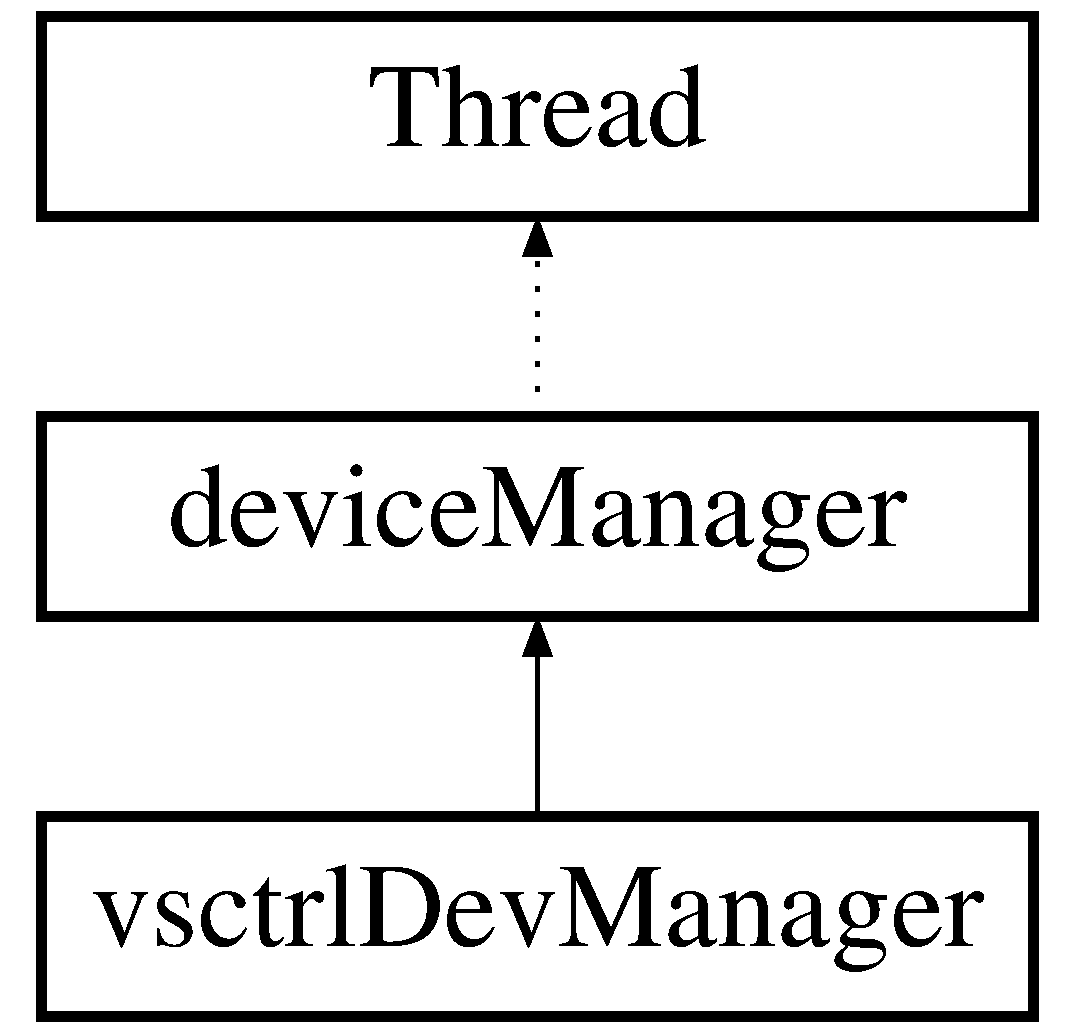
\includegraphics[height=3.000000cm]{classvsctrlDevManager}
\end{center}
\end{figure}
\subsection*{Public Member Functions}
\begin{DoxyCompactItemize}
\item 
\hypertarget{classvsctrlDevManager_a089d585fca4be21726d0708977abc7e4}{void {\bfseries print\-Biases} ()}\label{classvsctrlDevManager_a089d585fca4be21726d0708977abc7e4}

\item 
\hypertarget{classvsctrlDevManager_a4942068d2a90273bf333b9c5bd4bca1c}{unsigned int {\bfseries get\-Bias} (std\-::string bias\-Name)}\label{classvsctrlDevManager_a4942068d2a90273bf333b9c5bd4bca1c}

\item 
\hypertarget{classvsctrlDevManager_aee610b6b7e574e4763b15e1993e9ef4b}{virtual bool {\bfseries open\-Device} ()}\label{classvsctrlDevManager_aee610b6b7e574e4763b15e1993e9ef4b}

\item 
\hypertarget{classvsctrlDevManager_a5ca1d208ff16147546fd918af0a18cda}{virtual void {\bfseries close\-Device} ()}\label{classvsctrlDevManager_a5ca1d208ff16147546fd918af0a18cda}

\item 
\hypertarget{classvsctrlDevManager_ab54ace30b1bd3398fc951e82745f38aa}{{\bfseries vsctrl\-Dev\-Manager} (std\-::string channel, std\-::string chip)}\label{classvsctrlDevManager_ab54ace30b1bd3398fc951e82745f38aa}

\item 
\hypertarget{classvsctrlDevManager_a9db8592ea35fc47134c0a7d3e261462d}{int {\bfseries chip\-Reset} ()}\label{classvsctrlDevManager_a9db8592ea35fc47134c0a7d3e261462d}

\item 
\hypertarget{classvsctrlDevManager_aaffe2de0b0b855eaf69aa8d26ca8adfb}{int {\bfseries chip\-Power\-Down} ()}\label{classvsctrlDevManager_aaffe2de0b0b855eaf69aa8d26ca8adfb}

\item 
\hypertarget{classvsctrlDevManager_a26ee4e76e8691abcf9bf01fb1943aa5e}{int {\bfseries chip\-Power\-Up} ()}\label{classvsctrlDevManager_a26ee4e76e8691abcf9bf01fb1943aa5e}

\item 
\hypertarget{classvsctrlDevManager_aa9d0e1ebe2852643821a903769c72a88}{int {\bfseries get\-Fpga\-Status} ()}\label{classvsctrlDevManager_aa9d0e1ebe2852643821a903769c72a88}

\item 
\hypertarget{classvsctrlDevManager_a34310dcff72b9c9f4f2a80fb7ab25a0a}{int {\bfseries clear\-Fpga\-Status} (std\-::string clr)}\label{classvsctrlDevManager_a34310dcff72b9c9f4f2a80fb7ab25a0a}

\item 
\hypertarget{classvsctrlDevManager_a55353e0f83e3b3020ea151ddd8e7f14f}{int {\bfseries get\-Fpga\-Rel} ()}\label{classvsctrlDevManager_a55353e0f83e3b3020ea151ddd8e7f14f}

\item 
\hypertarget{classvsctrlDevManager_a1718274a8e09640d01a6e1c30b81dea3}{int {\bfseries get\-Fpga\-Info} ()}\label{classvsctrlDevManager_a1718274a8e09640d01a6e1c30b81dea3}

\item 
\hypertarget{classvsctrlDevManager_a09e8586d71ef063d025a37a1a6977310}{int {\bfseries write\-Aer\-Timings} (uint8\-\_\-t ack\-\_\-rel, uint8\-\_\-t sample, uint8\-\_\-t ack\-\_\-set)}\label{classvsctrlDevManager_a09e8586d71ef063d025a37a1a6977310}

\item 
\hypertarget{classvsctrlDevManager_aed1443c969692cd042d87997a59a2479}{int {\bfseries write\-Bg\-Timings} (uint8\-\_\-t prescaler, uint8\-\_\-t hold, uint8\-\_\-t ck\-\_\-active, uint8\-\_\-t latch\-\_\-setup, uint8\-\_\-t latch\-\_\-active)}\label{classvsctrlDevManager_aed1443c969692cd042d87997a59a2479}

\item 
\hypertarget{classvsctrlDevManager_a821576ea67f67432d584c19abd20005c}{int {\bfseries get\-Bg\-Timings} ()}\label{classvsctrlDevManager_a821576ea67f67432d584c19abd20005c}

\item 
\hypertarget{classvsctrlDevManager_aa898c4407bfe7e1f53ea04c45ca2ebd5}{int {\bfseries get\-Aer\-Timings} ()}\label{classvsctrlDevManager_aa898c4407bfe7e1f53ea04c45ca2ebd5}

\item 
\hypertarget{classvsctrlDevManager_a3c77d4aec1d1a05c4295a97372af4149}{int {\bfseries init\-Device} ()}\label{classvsctrlDevManager_a3c77d4aec1d1a05c4295a97372af4149}

\item 
\hypertarget{classvsctrlDevManager_aef5104292baec220c7a70ffdc7e2c016}{int {\bfseries write\-G\-P\-O\-Register} (uint32\-\_\-t data)}\label{classvsctrlDevManager_aef5104292baec220c7a70ffdc7e2c016}

\item 
\hypertarget{classvsctrlDevManager_a9e71984e46f46b72e43e08329cdbca94}{int {\bfseries read\-G\-P\-O\-Register} ()}\label{classvsctrlDevManager_a9e71984e46f46b72e43e08329cdbca94}

\item 
\hypertarget{classvsctrlDevManager_a559222224b7f13e14f0a80ba327bbb27}{bool {\bfseries program\-Biases} ()}\label{classvsctrlDevManager_a559222224b7f13e14f0a80ba327bbb27}

\item 
\hypertarget{classvsctrlDevManager_a086729caaeb04be43699fe5292c44e25}{bool {\bfseries set\-Bias} (std\-::string bias\-Name, unsigned int bias\-Value)}\label{classvsctrlDevManager_a086729caaeb04be43699fe5292c44e25}

\item 
\hypertarget{classvsctrlDevManager_a558be9af52147baee357e9c1a28b2268}{bool {\bfseries set\-Bias} (yarp\-::os\-::\-Bottle bias)}\label{classvsctrlDevManager_a558be9af52147baee357e9c1a28b2268}

\end{DoxyCompactItemize}
\subsection*{Additional Inherited Members}


The documentation for this class was generated from the following files\-:\begin{DoxyCompactItemize}
\item 
/home/aglover/workspace/projects/event\-Driven/src/grabbers/zynq\-Grabber/include/i\-Cub/device\-Manager.\-h\item 
/home/aglover/workspace/projects/event\-Driven/src/grabbers/zynq\-Grabber/src/device\-Manager.\-cpp\end{DoxyCompactItemize}

\hypertarget{classemorph_1_1vSurface}{\section{emorph\-:\-:v\-Surface Class Reference}
\label{classemorph_1_1vSurface}\index{emorph\-::v\-Surface@{emorph\-::v\-Surface}}
}


The \hyperlink{classemorph_1_1vWindow}{v\-Window} class holds a list of events for a period of time as specified. Event expiry is checked each time new events are added and expired events are removed. At any point in time a copy of the current list of events can be requested.  




{\ttfamily \#include $<$v\-Surface.\-h$>$}

\subsection*{Public Member Functions}
\begin{DoxyCompactItemize}
\item 
\hyperlink{classemorph_1_1vSurface_a7cd409f3b050a8cfbf9293284741eb6f}{v\-Surface} (int width=128, int height=128)
\begin{DoxyCompactList}\small\item\em \hyperlink{classemorph_1_1vWindow}{v\-Window} constructor \end{DoxyCompactList}\item 
\hypertarget{classemorph_1_1vSurface_a16d06483fa8a093bc1676c97deb9a074}{{\bfseries v\-Surface} (const \hyperlink{classemorph_1_1vSurface}{v\-Surface} \&)}\label{classemorph_1_1vSurface_a16d06483fa8a093bc1676c97deb9a074}

\item 
\hypertarget{classemorph_1_1vSurface_ad5f34493d533520c6913f9b938bc1f62}{\hyperlink{classemorph_1_1vSurface}{v\-Surface} {\bfseries operator=} (const \hyperlink{classemorph_1_1vSurface}{v\-Surface} \&)}\label{classemorph_1_1vSurface_ad5f34493d533520c6913f9b938bc1f62}

\item 
\hyperlink{classemorph_1_1vEvent}{v\-Event} $\ast$ \hyperlink{classemorph_1_1vSurface_aeb801c9d1a4b5c801b389a7f9ef9b82d}{add\-Event} (\hyperlink{classemorph_1_1AddressEvent}{emorph\-::\-Address\-Event} \&event)
\begin{DoxyCompactList}\small\item\em add\-Event adds an event to the window. Also checks for expired events. \end{DoxyCompactList}\item 
\hyperlink{classemorph_1_1vEvent}{v\-Event} $\ast$ \hyperlink{classemorph_1_1vSurface_ad348c7b75c0cb7530af3835021ef101e}{get\-Most\-Recent} ()
\begin{DoxyCompactList}\small\item\em get\-Most\-Recent \end{DoxyCompactList}\item 
\hypertarget{classemorph_1_1vSurface_a51d798ee57bbd56df9644b9dacd7e4b7}{void {\bfseries clear} ()}\label{classemorph_1_1vSurface_a51d798ee57bbd56df9644b9dacd7e4b7}

\item 
\hypertarget{classemorph_1_1vSurface_af7b1bfed295daca8e16ec4f563470b54}{const \hyperlink{classemorph_1_1vQueue}{v\-Queue} \& {\bfseries get\-S\-U\-R\-F} (int d)}\label{classemorph_1_1vSurface_af7b1bfed295daca8e16ec4f563470b54}

\item 
\hypertarget{classemorph_1_1vSurface_ae0095a43c5848a2fa8602aa5f9ad2040}{const \hyperlink{classemorph_1_1vQueue}{v\-Queue} \& {\bfseries get\-S\-U\-R\-F} (int x, int y, int d)}\label{classemorph_1_1vSurface_ae0095a43c5848a2fa8602aa5f9ad2040}

\item 
\hypertarget{classemorph_1_1vSurface_ad4b09e955e93cad783cd1fa137cfcb73}{const \hyperlink{classemorph_1_1vQueue}{v\-Queue} \& {\bfseries get\-S\-U\-R\-F} (int xl, int xh, int yl, int yh)}\label{classemorph_1_1vSurface_ad4b09e955e93cad783cd1fa137cfcb73}

\end{DoxyCompactItemize}


\subsection{Detailed Description}
The \hyperlink{classemorph_1_1vWindow}{v\-Window} class holds a list of events for a period of time as specified. Event expiry is checked each time new events are added and expired events are removed. At any point in time a copy of the current list of events can be requested. 

\subsection{Constructor \& Destructor Documentation}
\hypertarget{classemorph_1_1vSurface_a7cd409f3b050a8cfbf9293284741eb6f}{\index{emorph\-::v\-Surface@{emorph\-::v\-Surface}!v\-Surface@{v\-Surface}}
\index{v\-Surface@{v\-Surface}!emorph::vSurface@{emorph\-::v\-Surface}}
\subsubsection[{v\-Surface}]{\setlength{\rightskip}{0pt plus 5cm}emorph\-::v\-Surface\-::v\-Surface (
\begin{DoxyParamCaption}
\item[{int}]{width = {\ttfamily 128}, }
\item[{int}]{height = {\ttfamily 128}}
\end{DoxyParamCaption}
)}}\label{classemorph_1_1vSurface_a7cd409f3b050a8cfbf9293284741eb6f}


\hyperlink{classemorph_1_1vWindow}{v\-Window} constructor 


\begin{DoxyParams}{Parameters}
{\em window\-Size} & optional time to store events (in us) \\
\hline
\end{DoxyParams}


\subsection{Member Function Documentation}
\hypertarget{classemorph_1_1vSurface_aeb801c9d1a4b5c801b389a7f9ef9b82d}{\index{emorph\-::v\-Surface@{emorph\-::v\-Surface}!add\-Event@{add\-Event}}
\index{add\-Event@{add\-Event}!emorph::vSurface@{emorph\-::v\-Surface}}
\subsubsection[{add\-Event}]{\setlength{\rightskip}{0pt plus 5cm}{\bf v\-Event} $\ast$ emorph\-::v\-Surface\-::add\-Event (
\begin{DoxyParamCaption}
\item[{{\bf emorph\-::\-Address\-Event} \&}]{event}
\end{DoxyParamCaption}
)}}\label{classemorph_1_1vSurface_aeb801c9d1a4b5c801b389a7f9ef9b82d}


add\-Event adds an event to the window. Also checks for expired events. 


\begin{DoxyParams}{Parameters}
{\em event} & the event to add \\
\hline
\end{DoxyParams}
\hypertarget{classemorph_1_1vSurface_ad348c7b75c0cb7530af3835021ef101e}{\index{emorph\-::v\-Surface@{emorph\-::v\-Surface}!get\-Most\-Recent@{get\-Most\-Recent}}
\index{get\-Most\-Recent@{get\-Most\-Recent}!emorph::vSurface@{emorph\-::v\-Surface}}
\subsubsection[{get\-Most\-Recent}]{\setlength{\rightskip}{0pt plus 5cm}{\bf v\-Event} $\ast$ emorph\-::v\-Surface\-::get\-Most\-Recent (
\begin{DoxyParamCaption}
{}
\end{DoxyParamCaption}
)}}\label{classemorph_1_1vSurface_ad348c7b75c0cb7530af3835021ef101e}


get\-Most\-Recent 

\begin{DoxyReturn}{Returns}

\end{DoxyReturn}


The documentation for this class was generated from the following files\-:\begin{DoxyCompactItemize}
\item 
/home/aglover/workspace/projects/event\-Driven/emorph\-\_\-lib/include/i\-Cub/emorph/v\-Surface.\-h\item 
/home/aglover/workspace/projects/event\-Driven/emorph\-\_\-lib/src/v\-Surface.\-cpp\end{DoxyCompactItemize}

\hypertarget{classvTemplateModule}{\section{v\-Template\-Module Class Reference}
\label{classvTemplateModule}\index{v\-Template\-Module@{v\-Template\-Module}}
}
Inheritance diagram for v\-Template\-Module\-:\begin{figure}[H]
\begin{center}
\leavevmode
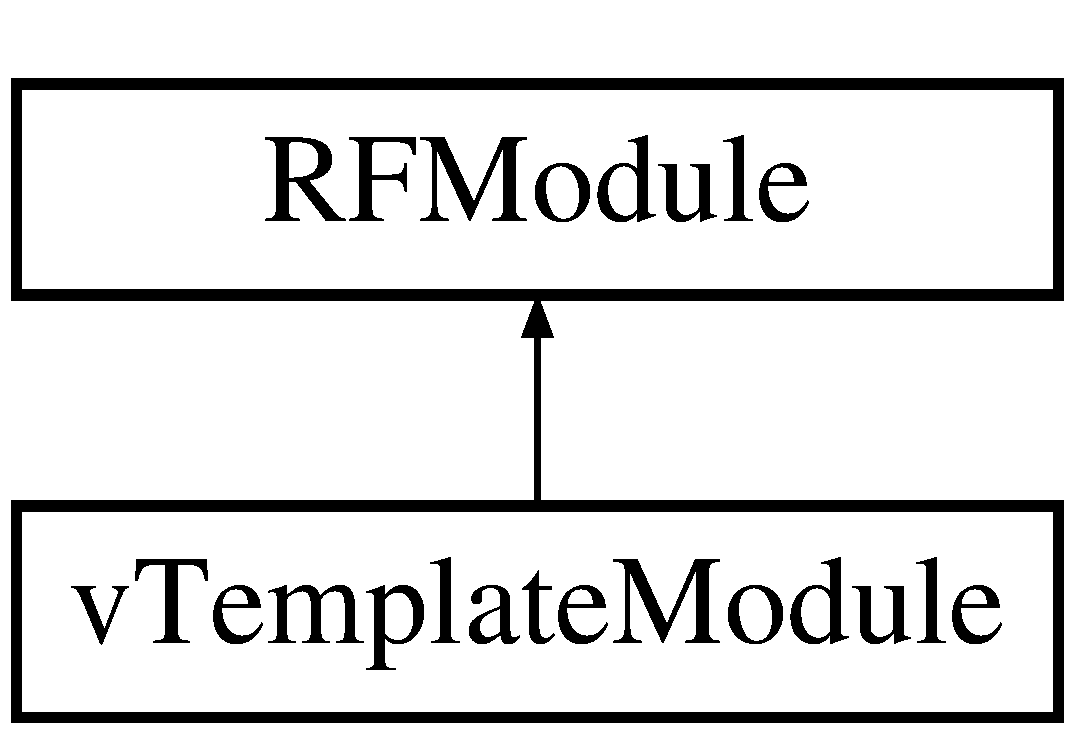
\includegraphics[height=2.000000cm]{classvTemplateModule}
\end{center}
\end{figure}
\subsection*{Public Member Functions}
\begin{DoxyCompactItemize}
\item 
\hypertarget{classvTemplateModule_ac673213dfbb34f1719a8a17b5549f3ab}{virtual bool {\bfseries configure} (yarp\-::os\-::\-Resource\-Finder \&rf)}\label{classvTemplateModule_ac673213dfbb34f1719a8a17b5549f3ab}

\item 
\hypertarget{classvTemplateModule_a4104e88622abbd133df02af82988a167}{virtual bool {\bfseries interrupt\-Module} ()}\label{classvTemplateModule_a4104e88622abbd133df02af82988a167}

\item 
\hypertarget{classvTemplateModule_ac94b9d709bf56efac2a9f82f393843dc}{virtual bool {\bfseries close} ()}\label{classvTemplateModule_ac94b9d709bf56efac2a9f82f393843dc}

\item 
\hypertarget{classvTemplateModule_aa2e6141f31e4cea8f94f0b5a1b08a934}{virtual bool {\bfseries respond} (const yarp\-::os\-::\-Bottle \&command, yarp\-::os\-::\-Bottle \&reply)}\label{classvTemplateModule_aa2e6141f31e4cea8f94f0b5a1b08a934}

\item 
\hypertarget{classvTemplateModule_a691e4424b5de4ee43e249421a24a87cb}{virtual double {\bfseries get\-Period} ()}\label{classvTemplateModule_a691e4424b5de4ee43e249421a24a87cb}

\item 
\hypertarget{classvTemplateModule_abd78b6b36cc849bbc34d6a3033cc4654}{virtual bool {\bfseries update\-Module} ()}\label{classvTemplateModule_abd78b6b36cc849bbc34d6a3033cc4654}

\end{DoxyCompactItemize}


The documentation for this class was generated from the following files\-:\begin{DoxyCompactItemize}
\item 
/home/aglover/workspace/projects/event\-Driven/src/processing/template/include/v\-Template.\-h\item 
/home/aglover/workspace/projects/event\-Driven/src/processing/template/src/v\-Template.\-cpp\end{DoxyCompactItemize}

\hypertarget{classvTrackToRobotManager}{\section{v\-Track\-To\-Robot\-Manager Class Reference}
\label{classvTrackToRobotManager}\index{v\-Track\-To\-Robot\-Manager@{v\-Track\-To\-Robot\-Manager}}
}
Inheritance diagram for v\-Track\-To\-Robot\-Manager\-:\begin{figure}[H]
\begin{center}
\leavevmode
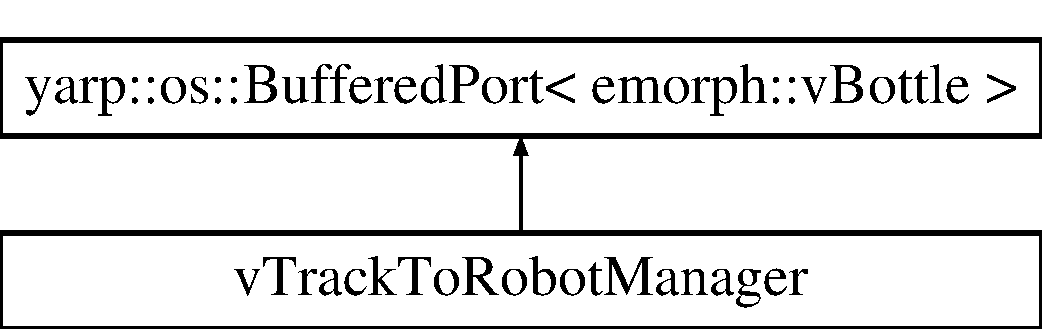
\includegraphics[height=2.000000cm]{classvTrackToRobotManager}
\end{center}
\end{figure}
\subsection*{Public Member Functions}
\begin{DoxyCompactItemize}
\item 
\hypertarget{classvTrackToRobotManager_ae3a3a2b0145f05c001169efa52c9a101}{bool {\bfseries set\-Method} (std\-::string methodname)}\label{classvTrackToRobotManager_ae3a3a2b0145f05c001169efa52c9a101}

\item 
\hypertarget{classvTrackToRobotManager_acd829a9e8130d24812666a2738926468}{bool {\bfseries open} (const std\-::string \&name)}\label{classvTrackToRobotManager_acd829a9e8130d24812666a2738926468}

\item 
\hypertarget{classvTrackToRobotManager_a96a625860ae11797ed9506f53b9f70f2}{void {\bfseries on\-Read} (\hyperlink{classemorph_1_1vBottle}{emorph\-::v\-Bottle} \&bot)}\label{classvTrackToRobotManager_a96a625860ae11797ed9506f53b9f70f2}

\item 
\hypertarget{classvTrackToRobotManager_a3d413d0808aeef12be32541cd2e892ed}{void {\bfseries interrupt} ()}\label{classvTrackToRobotManager_a3d413d0808aeef12be32541cd2e892ed}

\item 
\hypertarget{classvTrackToRobotManager_a2d43766cdec75aa97d064276c17ee81c}{void {\bfseries close} ()}\label{classvTrackToRobotManager_a2d43766cdec75aa97d064276c17ee81c}

\end{DoxyCompactItemize}


The documentation for this class was generated from the following files\-:\begin{DoxyCompactItemize}
\item 
/home/aglover/workspace/projects/event\-Driven/src/movement/v\-Track\-To\-Robot/include/v\-Track\-To\-Robot.\-h\item 
/home/aglover/workspace/projects/event\-Driven/src/movement/v\-Track\-To\-Robot/src/v\-Track\-To\-Robot.\-cpp\end{DoxyCompactItemize}

\hypertarget{classvTrackToRobotModule}{\section{v\-Track\-To\-Robot\-Module Class Reference}
\label{classvTrackToRobotModule}\index{v\-Track\-To\-Robot\-Module@{v\-Track\-To\-Robot\-Module}}
}
Inheritance diagram for v\-Track\-To\-Robot\-Module\-:\begin{figure}[H]
\begin{center}
\leavevmode
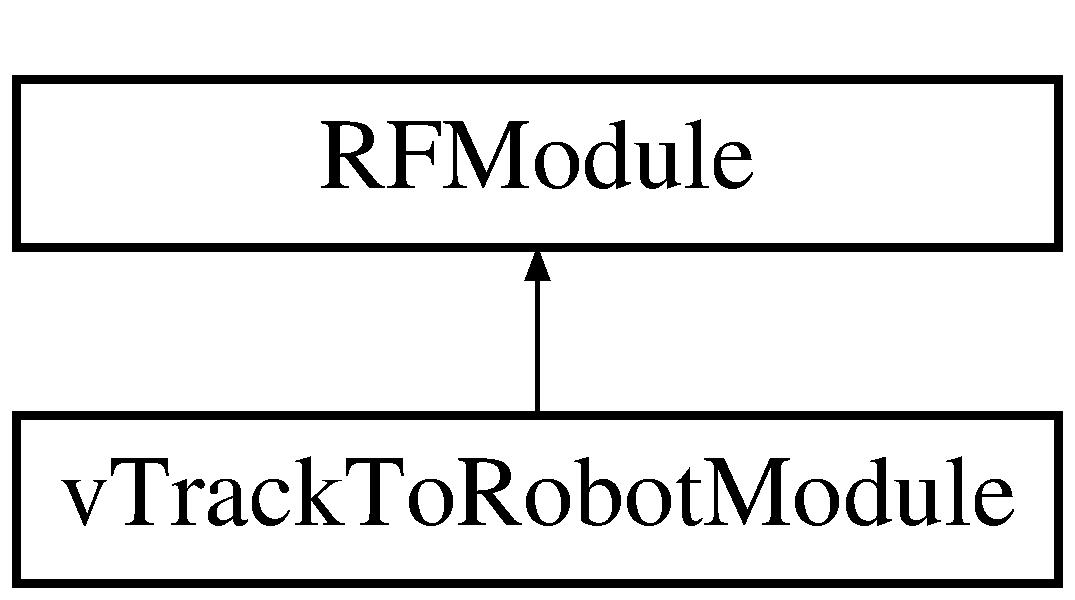
\includegraphics[height=2.000000cm]{classvTrackToRobotModule}
\end{center}
\end{figure}
\subsection*{Public Member Functions}
\begin{DoxyCompactItemize}
\item 
\hypertarget{classvTrackToRobotModule_ac724b3b5b9a538f211b062d2adf0118d}{virtual bool {\bfseries configure} (yarp\-::os\-::\-Resource\-Finder \&rf)}\label{classvTrackToRobotModule_ac724b3b5b9a538f211b062d2adf0118d}

\item 
\hypertarget{classvTrackToRobotModule_ae91ddadef668498e269699c848d388b1}{virtual bool {\bfseries interrupt\-Module} ()}\label{classvTrackToRobotModule_ae91ddadef668498e269699c848d388b1}

\item 
\hypertarget{classvTrackToRobotModule_a82d1ba0a15150dd2763b61cd80a33b1c}{virtual bool {\bfseries close} ()}\label{classvTrackToRobotModule_a82d1ba0a15150dd2763b61cd80a33b1c}

\item 
\hypertarget{classvTrackToRobotModule_adb673c97a3c36730d5d7a36da24a32e7}{virtual double {\bfseries get\-Period} ()}\label{classvTrackToRobotModule_adb673c97a3c36730d5d7a36da24a32e7}

\item 
\hypertarget{classvTrackToRobotModule_ada6ea3de8172c79d5f3a63b79db0c220}{virtual bool {\bfseries update\-Module} ()}\label{classvTrackToRobotModule_ada6ea3de8172c79d5f3a63b79db0c220}

\end{DoxyCompactItemize}


The documentation for this class was generated from the following files\-:\begin{DoxyCompactItemize}
\item 
/home/aglover/workspace/projects/event\-Driven/src/movement/v\-Track\-To\-Robot/include/v\-Track\-To\-Robot.\-h\item 
/home/aglover/workspace/projects/event\-Driven/src/movement/v\-Track\-To\-Robot/src/v\-Track\-To\-Robot.\-cpp\end{DoxyCompactItemize}

\hypertarget{classemorph_1_1vtsHelper}{\section{emorph\-:\-:vts\-Helper Class Reference}
\label{classemorph_1_1vtsHelper}\index{emorph\-::vts\-Helper@{emorph\-::vts\-Helper}}
}
\subsection*{Public Member Functions}
\begin{DoxyCompactItemize}
\item 
\hypertarget{classemorph_1_1vtsHelper_afc51549e5a47ec249359360980964361}{unsigned long int {\bfseries operator()} (int timestamp)}\label{classemorph_1_1vtsHelper_afc51549e5a47ec249359360980964361}

\end{DoxyCompactItemize}
\subsection*{Static Public Member Functions}
\begin{DoxyCompactItemize}
\item 
\hypertarget{classemorph_1_1vtsHelper_a272802b997c7957e35bca9171dd9b67f}{static long int {\bfseries max\-Stamp} ()}\label{classemorph_1_1vtsHelper_a272802b997c7957e35bca9171dd9b67f}

\item 
\hypertarget{classemorph_1_1vtsHelper_afff75520a8c7147c9d96b988ffd1c457}{static double {\bfseries tstosecs} ()}\label{classemorph_1_1vtsHelper_afff75520a8c7147c9d96b988ffd1c457}

\end{DoxyCompactItemize}


The documentation for this class was generated from the following file\-:\begin{DoxyCompactItemize}
\item 
/home/aglover/workspace/projects/event\-Driven/emorph\-\_\-lib/include/i\-Cub/emorph/vts\-Helper.\-h\end{DoxyCompactItemize}

\hypertarget{classvUndistortModule}{\section{v\-Undistort\-Module Class Reference}
\label{classvUndistortModule}\index{v\-Undistort\-Module@{v\-Undistort\-Module}}
}
Inheritance diagram for v\-Undistort\-Module\-:\begin{figure}[H]
\begin{center}
\leavevmode
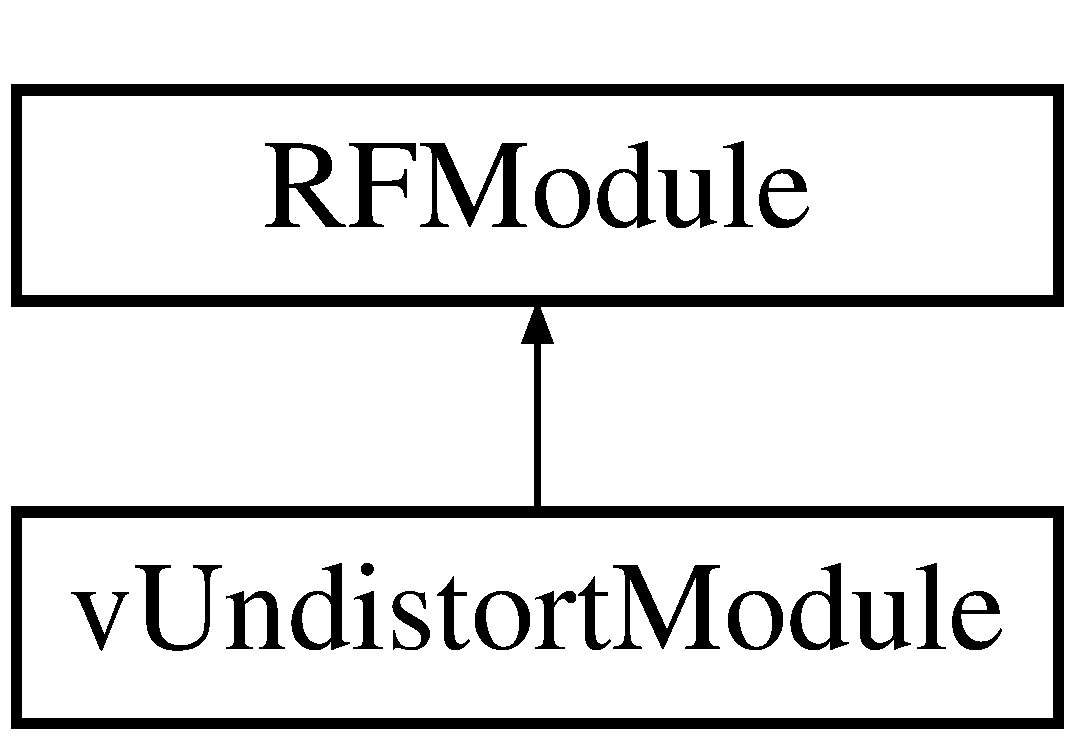
\includegraphics[height=2.000000cm]{classvUndistortModule}
\end{center}
\end{figure}
\subsection*{Public Member Functions}
\begin{DoxyCompactItemize}
\item 
\hypertarget{classvUndistortModule_a9f4fce79ccdc9e9b3b2269c4d94beb22}{virtual bool {\bfseries configure} (yarp\-::os\-::\-Resource\-Finder \&rf)}\label{classvUndistortModule_a9f4fce79ccdc9e9b3b2269c4d94beb22}

\item 
\hypertarget{classvUndistortModule_ab552bfdeddb57cb1cb332169761571d8}{virtual bool {\bfseries interrupt\-Module} ()}\label{classvUndistortModule_ab552bfdeddb57cb1cb332169761571d8}

\item 
\hypertarget{classvUndistortModule_a03d2de14720d332b0bbafe5b200f3ce0}{virtual bool {\bfseries close} ()}\label{classvUndistortModule_a03d2de14720d332b0bbafe5b200f3ce0}

\item 
\hypertarget{classvUndistortModule_a11c58860f7bcd6783d8265b55b8a4fe9}{virtual bool {\bfseries respond} (const yarp\-::os\-::\-Bottle \&command, yarp\-::os\-::\-Bottle \&reply)}\label{classvUndistortModule_a11c58860f7bcd6783d8265b55b8a4fe9}

\item 
\hypertarget{classvUndistortModule_a8ec64be6e169a66a5c68aedb3f8618f0}{virtual double {\bfseries get\-Period} ()}\label{classvUndistortModule_a8ec64be6e169a66a5c68aedb3f8618f0}

\item 
\hypertarget{classvUndistortModule_a68a6946ee4bb8197ec555cf3d2f3b657}{virtual bool {\bfseries update\-Module} ()}\label{classvUndistortModule_a68a6946ee4bb8197ec555cf3d2f3b657}

\end{DoxyCompactItemize}


The documentation for this class was generated from the following files\-:\begin{DoxyCompactItemize}
\item 
/home/aglover/workspace/projects/event\-Driven/src/processing/v\-Undistort\-Cam/include/v\-Undistort\-Cam.\-h\item 
/home/aglover/workspace/projects/event\-Driven/src/processing/v\-Undistort\-Cam/src/v\-Undistort\-Cam.\-cpp\end{DoxyCompactItemize}

\hypertarget{classemorph_1_1vWindow}{\section{emorph\-:\-:v\-Window Class Reference}
\label{classemorph_1_1vWindow}\index{emorph\-::v\-Window@{emorph\-::v\-Window}}
}


The \hyperlink{classemorph_1_1vWindow}{v\-Window} class holds a list of events for a period of time as specified. Event expiry is checked each time new events are added and expired events are removed. At any point in time a copy of the current list of events can be requested.  




{\ttfamily \#include $<$v\-Window.\-h$>$}

\subsection*{Public Member Functions}
\begin{DoxyCompactItemize}
\item 
\hyperlink{classemorph_1_1vWindow_ae7e0ebcfb7ca683596a967246d609650}{v\-Window} (int width=128, int height=128, int duration=20000)
\begin{DoxyCompactList}\small\item\em \hyperlink{classemorph_1_1vWindow}{v\-Window} constructor \end{DoxyCompactList}\item 
\hypertarget{classemorph_1_1vWindow_a6f79791c8d68c07c73d0e8239be1e51e}{{\bfseries v\-Window} (const \hyperlink{classemorph_1_1vWindow}{v\-Window} \&)}\label{classemorph_1_1vWindow_a6f79791c8d68c07c73d0e8239be1e51e}

\item 
\hypertarget{classemorph_1_1vWindow_ae1cc66633b2fe2e8af91669a26e679d8}{\hyperlink{classemorph_1_1vWindow}{v\-Window} {\bfseries operator=} (const \hyperlink{classemorph_1_1vWindow}{v\-Window} \&)}\label{classemorph_1_1vWindow_ae1cc66633b2fe2e8af91669a26e679d8}

\item 
void \hyperlink{classemorph_1_1vWindow_aedf610895d1ed7d606e5ab403436f200}{set\-Temporal\-Window\-Size} (int duration)
\begin{DoxyCompactList}\small\item\em set\-Window\-Size sets the length of time to store events \end{DoxyCompactList}\item 
void \hyperlink{classemorph_1_1vWindow_ab64b89bf88b7f5460bcea85a0fe31e1c}{add\-Event} (\hyperlink{classemorph_1_1vEvent}{emorph\-::v\-Event} \&event)
\begin{DoxyCompactList}\small\item\em add\-Event adds an event to the window. Also checks for expired events. \end{DoxyCompactList}\item 
\hyperlink{classemorph_1_1vEvent}{v\-Event} $\ast$ \hyperlink{classemorph_1_1vWindow_a20c61b89d6ef1acad4e6c6d7bac89a5b}{get\-Most\-Recent} ()
\begin{DoxyCompactList}\small\item\em get\-Most\-Recent \end{DoxyCompactList}\item 
const \hyperlink{classemorph_1_1vQueue}{v\-Queue} \& \hyperlink{classemorph_1_1vWindow_a0866119cfd77cba8e5b62e0d7a4af195}{get\-T\-W} ()
\begin{DoxyCompactList}\small\item\em get\-Window \end{DoxyCompactList}\item 
\hypertarget{classemorph_1_1vWindow_a3b68c6c2fb8b1b5988b52f8703dff171}{void {\bfseries copy\-T\-W\-T\-O} (\hyperlink{classemorph_1_1vQueue}{v\-Queue} \&that)}\label{classemorph_1_1vWindow_a3b68c6c2fb8b1b5988b52f8703dff171}

\item 
const \hyperlink{classemorph_1_1vQueue}{v\-Queue} \& \hyperlink{classemorph_1_1vWindow_a49b43ccdd801608a72f962a2db9b9fc6}{get\-S\-T\-W} (int x, int y, int d)
\begin{DoxyCompactList}\small\item\em get\-Spatial\-Window returns Address\-Events within a spatial window \end{DoxyCompactList}\item 
const \hyperlink{classemorph_1_1vQueue}{v\-Queue} \& \hyperlink{classemorph_1_1vWindow_aa6691b1453a5abff9d16001b314ee3ae}{get\-S\-T\-W} (int xl, int xh, int yl, int yh)
\begin{DoxyCompactList}\small\item\em get\-Spatial\-Window returns Address\-Events within a spatial window \end{DoxyCompactList}\item 
\hypertarget{classemorph_1_1vWindow_a4ad3e6a65dea8ad0cf52b03ef41fe8fb}{const \hyperlink{classemorph_1_1vQueue}{v\-Queue} \& {\bfseries get\-S\-M\-A\-R\-T\-S\-T\-W} (int d)}\label{classemorph_1_1vWindow_a4ad3e6a65dea8ad0cf52b03ef41fe8fb}

\item 
\hypertarget{classemorph_1_1vWindow_ad03a49288c115cfec54462d356606033}{const \hyperlink{classemorph_1_1vQueue}{v\-Queue} \& {\bfseries get\-S\-U\-R\-F} (int pol)}\label{classemorph_1_1vWindow_ad03a49288c115cfec54462d356606033}

\item 
\hypertarget{classemorph_1_1vWindow_a7c4dd7d2f436537552b9d0c42c1263b3}{const \hyperlink{classemorph_1_1vQueue}{v\-Queue} \& {\bfseries get\-S\-M\-A\-R\-T\-S\-U\-R\-F} (int d)}\label{classemorph_1_1vWindow_a7c4dd7d2f436537552b9d0c42c1263b3}

\item 
\hypertarget{classemorph_1_1vWindow_a97de6f3768adfe0fe87c9d538effe944}{const \hyperlink{classemorph_1_1vQueue}{v\-Queue} \& {\bfseries get\-S\-U\-R\-F} (int x, int y, int d, int pol)}\label{classemorph_1_1vWindow_a97de6f3768adfe0fe87c9d538effe944}

\item 
\hypertarget{classemorph_1_1vWindow_ae73175dc01dfe590770deedc14057f28}{const \hyperlink{classemorph_1_1vQueue}{v\-Queue} \& {\bfseries get\-S\-U\-R\-F} (int xl, int xh, int yl, int yh, int pol)}\label{classemorph_1_1vWindow_ae73175dc01dfe590770deedc14057f28}

\end{DoxyCompactItemize}


\subsection{Detailed Description}
The \hyperlink{classemorph_1_1vWindow}{v\-Window} class holds a list of events for a period of time as specified. Event expiry is checked each time new events are added and expired events are removed. At any point in time a copy of the current list of events can be requested. 

\subsection{Constructor \& Destructor Documentation}
\hypertarget{classemorph_1_1vWindow_ae7e0ebcfb7ca683596a967246d609650}{\index{emorph\-::v\-Window@{emorph\-::v\-Window}!v\-Window@{v\-Window}}
\index{v\-Window@{v\-Window}!emorph::vWindow@{emorph\-::v\-Window}}
\subsubsection[{v\-Window}]{\setlength{\rightskip}{0pt plus 5cm}emorph\-::v\-Window\-::v\-Window (
\begin{DoxyParamCaption}
\item[{int}]{width = {\ttfamily 128}, }
\item[{int}]{height = {\ttfamily 128}, }
\item[{int}]{duration = {\ttfamily 20000}}
\end{DoxyParamCaption}
)}}\label{classemorph_1_1vWindow_ae7e0ebcfb7ca683596a967246d609650}


\hyperlink{classemorph_1_1vWindow}{v\-Window} constructor 


\begin{DoxyParams}{Parameters}
{\em window\-Size} & optional time to store events (in us) \\
\hline
\end{DoxyParams}


\subsection{Member Function Documentation}
\hypertarget{classemorph_1_1vWindow_ab64b89bf88b7f5460bcea85a0fe31e1c}{\index{emorph\-::v\-Window@{emorph\-::v\-Window}!add\-Event@{add\-Event}}
\index{add\-Event@{add\-Event}!emorph::vWindow@{emorph\-::v\-Window}}
\subsubsection[{add\-Event}]{\setlength{\rightskip}{0pt plus 5cm}void emorph\-::v\-Window\-::add\-Event (
\begin{DoxyParamCaption}
\item[{{\bf emorph\-::v\-Event} \&}]{event}
\end{DoxyParamCaption}
)}}\label{classemorph_1_1vWindow_ab64b89bf88b7f5460bcea85a0fe31e1c}


add\-Event adds an event to the window. Also checks for expired events. 


\begin{DoxyParams}{Parameters}
{\em event} & the event to add \\
\hline
\end{DoxyParams}
\hypertarget{classemorph_1_1vWindow_a20c61b89d6ef1acad4e6c6d7bac89a5b}{\index{emorph\-::v\-Window@{emorph\-::v\-Window}!get\-Most\-Recent@{get\-Most\-Recent}}
\index{get\-Most\-Recent@{get\-Most\-Recent}!emorph::vWindow@{emorph\-::v\-Window}}
\subsubsection[{get\-Most\-Recent}]{\setlength{\rightskip}{0pt plus 5cm}{\bf v\-Event} $\ast$ emorph\-::v\-Window\-::get\-Most\-Recent (
\begin{DoxyParamCaption}
{}
\end{DoxyParamCaption}
)}}\label{classemorph_1_1vWindow_a20c61b89d6ef1acad4e6c6d7bac89a5b}


get\-Most\-Recent 

\begin{DoxyReturn}{Returns}

\end{DoxyReturn}
\hypertarget{classemorph_1_1vWindow_a49b43ccdd801608a72f962a2db9b9fc6}{\index{emorph\-::v\-Window@{emorph\-::v\-Window}!get\-S\-T\-W@{get\-S\-T\-W}}
\index{get\-S\-T\-W@{get\-S\-T\-W}!emorph::vWindow@{emorph\-::v\-Window}}
\subsubsection[{get\-S\-T\-W}]{\setlength{\rightskip}{0pt plus 5cm}const {\bf v\-Queue} \& emorph\-::v\-Window\-::get\-S\-T\-W (
\begin{DoxyParamCaption}
\item[{int}]{x, }
\item[{int}]{y, }
\item[{int}]{d}
\end{DoxyParamCaption}
)}}\label{classemorph_1_1vWindow_a49b43ccdd801608a72f962a2db9b9fc6}


get\-Spatial\-Window returns Address\-Events within a spatial window 


\begin{DoxyParams}{Parameters}
{\em x} & x centre \\
\hline
{\em y} & y centre \\
\hline
{\em d} & distance of the half-\/length of a square window \\
\hline
\end{DoxyParams}
\begin{DoxyReturn}{Returns}
a \hyperlink{classemorph_1_1vQueue}{v\-Queue} containing a copy of the events 
\end{DoxyReturn}
\hypertarget{classemorph_1_1vWindow_aa6691b1453a5abff9d16001b314ee3ae}{\index{emorph\-::v\-Window@{emorph\-::v\-Window}!get\-S\-T\-W@{get\-S\-T\-W}}
\index{get\-S\-T\-W@{get\-S\-T\-W}!emorph::vWindow@{emorph\-::v\-Window}}
\subsubsection[{get\-S\-T\-W}]{\setlength{\rightskip}{0pt plus 5cm}const {\bf v\-Queue} \& emorph\-::v\-Window\-::get\-S\-T\-W (
\begin{DoxyParamCaption}
\item[{int}]{xl, }
\item[{int}]{xh, }
\item[{int}]{yl, }
\item[{int}]{yh}
\end{DoxyParamCaption}
)}}\label{classemorph_1_1vWindow_aa6691b1453a5abff9d16001b314ee3ae}


get\-Spatial\-Window returns Address\-Events within a spatial window 


\begin{DoxyParams}{Parameters}
{\em xl} & lower x value of window \\
\hline
{\em xh} & upper x value of window \\
\hline
{\em yl} & lower y value of window \\
\hline
{\em yh} & upper y value of window \\
\hline
\end{DoxyParams}
\begin{DoxyReturn}{Returns}
a \hyperlink{classemorph_1_1vQueue}{v\-Queue} containing a copy of the events 
\end{DoxyReturn}
\hypertarget{classemorph_1_1vWindow_a0866119cfd77cba8e5b62e0d7a4af195}{\index{emorph\-::v\-Window@{emorph\-::v\-Window}!get\-T\-W@{get\-T\-W}}
\index{get\-T\-W@{get\-T\-W}!emorph::vWindow@{emorph\-::v\-Window}}
\subsubsection[{get\-T\-W}]{\setlength{\rightskip}{0pt plus 5cm}const {\bf v\-Queue} \& emorph\-::v\-Window\-::get\-T\-W (
\begin{DoxyParamCaption}
{}
\end{DoxyParamCaption}
)}}\label{classemorph_1_1vWindow_a0866119cfd77cba8e5b62e0d7a4af195}


get\-Window 

\begin{DoxyReturn}{Returns}

\end{DoxyReturn}
\hypertarget{classemorph_1_1vWindow_aedf610895d1ed7d606e5ab403436f200}{\index{emorph\-::v\-Window@{emorph\-::v\-Window}!set\-Temporal\-Window\-Size@{set\-Temporal\-Window\-Size}}
\index{set\-Temporal\-Window\-Size@{set\-Temporal\-Window\-Size}!emorph::vWindow@{emorph\-::v\-Window}}
\subsubsection[{set\-Temporal\-Window\-Size}]{\setlength{\rightskip}{0pt plus 5cm}void emorph\-::v\-Window\-::set\-Temporal\-Window\-Size (
\begin{DoxyParamCaption}
\item[{int}]{duration}
\end{DoxyParamCaption}
)\hspace{0.3cm}{\ttfamily [inline]}}}\label{classemorph_1_1vWindow_aedf610895d1ed7d606e5ab403436f200}


set\-Window\-Size sets the length of time to store events 


\begin{DoxyParams}{Parameters}
{\em window\-Size} & the time period (in us) \\
\hline
\end{DoxyParams}


The documentation for this class was generated from the following files\-:\begin{DoxyCompactItemize}
\item 
/home/aglover/workspace/projects/event\-Driven/emorph\-\_\-lib/include/i\-Cub/emorph/v\-Window.\-h\item 
/home/aglover/workspace/projects/event\-Driven/emorph\-\_\-lib/src/v\-Window.\-cpp\end{DoxyCompactItemize}

\hypertarget{classyarp2device}{\section{yarp2device Class Reference}
\label{classyarp2device}\index{yarp2device@{yarp2device}}
}
Inheritance diagram for yarp2device\-:\begin{figure}[H]
\begin{center}
\leavevmode
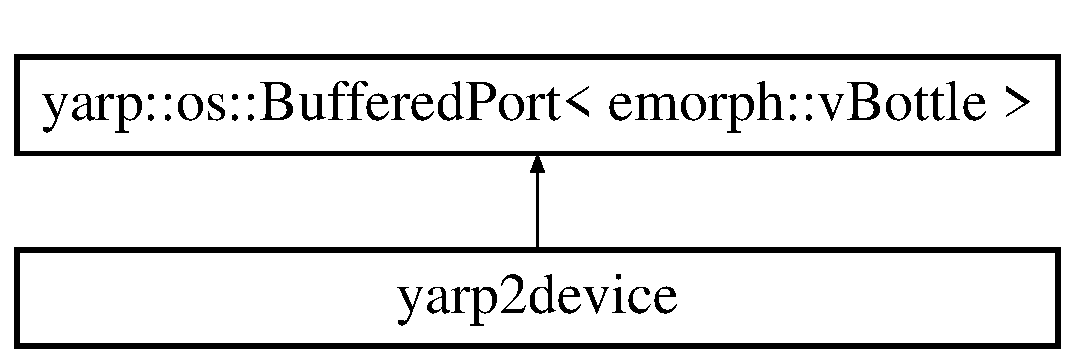
\includegraphics[height=2.000000cm]{classyarp2device}
\end{center}
\end{figure}
\subsection*{Public Member Functions}
\begin{DoxyCompactItemize}
\item 
\hypertarget{classyarp2device_a664050547336bee12457bb4c346727a6}{virtual bool {\bfseries open} (std\-::string module\-Name)}\label{classyarp2device_a664050547336bee12457bb4c346727a6}

\item 
\hypertarget{classyarp2device_a56b9560746d5dec6168f62426b302598}{bool {\bfseries init} ()}\label{classyarp2device_a56b9560746d5dec6168f62426b302598}

\item 
\hypertarget{classyarp2device_a4031dba4c05576ca4f444fe496fd1f42}{void {\bfseries close} ()}\label{classyarp2device_a4031dba4c05576ca4f444fe496fd1f42}

\item 
\hypertarget{classyarp2device_a0c5a6e14866a7cb8002bfa87fd293059}{void {\bfseries on\-Read} (\hyperlink{classemorph_1_1vBottle}{emorph\-::v\-Bottle} \&bot)}\label{classyarp2device_a0c5a6e14866a7cb8002bfa87fd293059}

\item 
\hypertarget{classyarp2device_ad2c4ae1fdb9839805c806d0084fdd20a}{void {\bfseries interrupt} ()}\label{classyarp2device_ad2c4ae1fdb9839805c806d0084fdd20a}

\item 
\hypertarget{classyarp2device_ab7e89f9acbec43013529e014162ce902}{void {\bfseries attach\-Device\-Manager} (\hyperlink{classdeviceManager}{device\-Manager} $\ast$dev\-Manager)}\label{classyarp2device_ab7e89f9acbec43013529e014162ce902}

\end{DoxyCompactItemize}


The documentation for this class was generated from the following files\-:\begin{DoxyCompactItemize}
\item 
/home/aglover/workspace/projects/event\-Driven/src/grabbers/zynq\-Grabber/include/i\-Cub/yarp2device.\-h\item 
/home/aglover/workspace/projects/event\-Driven/src/grabbers/zynq\-Grabber/src/yarp2device.\-cpp\end{DoxyCompactItemize}

\hypertarget{classzynqGrabberModule}{\section{zynq\-Grabber\-Module Class Reference}
\label{classzynqGrabberModule}\index{zynq\-Grabber\-Module@{zynq\-Grabber\-Module}}
}
Inheritance diagram for zynq\-Grabber\-Module\-:\begin{figure}[H]
\begin{center}
\leavevmode
\includegraphics[height=2.000000cm]{classzynqGrabberModule}
\end{center}
\end{figure}
\subsection*{Public Member Functions}
\begin{DoxyCompactItemize}
\item 
\hypertarget{classzynqGrabberModule_a2733856709df020d264750ce5afbe552}{bool {\bfseries configure} (yarp\-::os\-::\-Resource\-Finder \&rf)}\label{classzynqGrabberModule_a2733856709df020d264750ce5afbe552}

\item 
\hypertarget{classzynqGrabberModule_aa33152e027843920826ea02f323df8dd}{bool {\bfseries interrupt\-Module} ()}\label{classzynqGrabberModule_aa33152e027843920826ea02f323df8dd}

\item 
\hypertarget{classzynqGrabberModule_ae687b7063d3974a71a27a4cae8104480}{bool {\bfseries close} ()}\label{classzynqGrabberModule_ae687b7063d3974a71a27a4cae8104480}

\item 
\hypertarget{classzynqGrabberModule_afb439f66ef1786b6b503597dd6e74f33}{bool {\bfseries respond} (const yarp\-::os\-::\-Bottle \&command, yarp\-::os\-::\-Bottle \&reply)}\label{classzynqGrabberModule_afb439f66ef1786b6b503597dd6e74f33}

\item 
\hypertarget{classzynqGrabberModule_a584429a662fd6eb0b11d77294c1b40a5}{double {\bfseries get\-Period} ()}\label{classzynqGrabberModule_a584429a662fd6eb0b11d77294c1b40a5}

\item 
\hypertarget{classzynqGrabberModule_a53679eefbe74aa164fde84f9381450bc}{bool {\bfseries update\-Module} ()}\label{classzynqGrabberModule_a53679eefbe74aa164fde84f9381450bc}

\end{DoxyCompactItemize}


The documentation for this class was generated from the following files\-:\begin{DoxyCompactItemize}
\item 
/home/aglover/workspace/projects/event\-Driven/src/grabbers/zynq\-Grabber/include/i\-Cub/zynq\-Grabber\-Module.\-h\item 
/home/aglover/workspace/projects/event\-Driven/src/grabbers/zynq\-Grabber/src/\hyperlink{zynqGrabberModule_8cpp}{zynq\-Grabber\-Module.\-cpp}\end{DoxyCompactItemize}

\chapter{File Documentation}
\hypertarget{config_8h}{\section{/home/aglover/workspace/projects/event\-Driven/src/grabbers/aex\-Grabber/include/i\-Cub/config.h File Reference}
\label{config_8h}\index{/home/aglover/workspace/projects/event\-Driven/src/grabbers/aex\-Grabber/include/i\-Cub/config.\-h@{/home/aglover/workspace/projects/event\-Driven/src/grabbers/aex\-Grabber/include/i\-Cub/config.\-h}}
}


Simple header file for configuration. Intentionally separated for estetic purposes.  


\subsection*{Macros}
\begin{DoxyCompactItemize}
\item 
\hypertarget{config_8h_ad49b36abd5473a87913e4964cc1564c9}{\#define {\bfseries S\-I\-Z\-E\-\_\-\-O\-F\-\_\-\-E\-V\-E\-N\-T}~2048}\label{config_8h_ad49b36abd5473a87913e4964cc1564c9}

\item 
\hypertarget{config_8h_a458727ba44329288f712b89a0b52199a}{\#define {\bfseries S\-I\-Z\-E\-\_\-\-O\-F\-\_\-\-D\-A\-T\-A}~16384}\label{config_8h_a458727ba44329288f712b89a0b52199a}

\item 
\hypertarget{config_8h_a5da43425fff36347c69fc3c090e42c6c}{\#define {\bfseries S\-L\-O\-W}}\label{config_8h_a5da43425fff36347c69fc3c090e42c6c}

\end{DoxyCompactItemize}


\subsection{Detailed Description}
Simple header file for configuration. Intentionally separated for estetic purposes. 
\hypertarget{sending__buffer_8h}{\section{/home/aglover/workspace/projects/event\-Driven/src/grabbers/aex\-Grabber/include/i\-Cub/sending\-\_\-buffer.h File Reference}
\label{sending__buffer_8h}\index{/home/aglover/workspace/projects/event\-Driven/src/grabbers/aex\-Grabber/include/i\-Cub/sending\-\_\-buffer.\-h@{/home/aglover/workspace/projects/event\-Driven/src/grabbers/aex\-Grabber/include/i\-Cub/sending\-\_\-buffer.\-h}}
}


Sends the buffer (readings of cameras) on a Y\-A\-R\-P port.  


{\ttfamily \#include $<$yarp/os/\-Portable.\-h$>$}\\*
{\ttfamily \#include $<$yarp/os/\-Connection\-Writer.\-h$>$}\\*
{\ttfamily \#include $<$cstring$>$}\\*
{\ttfamily \#include \char`\"{}config.\-h\char`\"{}}\\*
\subsection*{Classes}
\begin{DoxyCompactItemize}
\item 
class \hyperlink{classsendingBuffer}{sending\-Buffer}
\end{DoxyCompactItemize}


\subsection{Detailed Description}
Sends the buffer (readings of cameras) on a Y\-A\-R\-P port. Sends information on a Y\-A\-R\-P port (see header \hyperlink{sending__buffer_8h}{sending\-\_\-buffer.\-h})
\hypertarget{aexGrabberModule_8cpp}{\section{/home/aglover/workspace/projects/event\-Driven/src/grabbers/aex\-Grabber/src/aex\-Grabber\-Module.cpp File Reference}
\label{aexGrabberModule_8cpp}\index{/home/aglover/workspace/projects/event\-Driven/src/grabbers/aex\-Grabber/src/aex\-Grabber\-Module.\-cpp@{/home/aglover/workspace/projects/event\-Driven/src/grabbers/aex\-Grabber/src/aex\-Grabber\-Module.\-cpp}}
}


Implementation of the \hyperlink{classaexGrabberModule}{aex\-Grabber\-Module} (see header file).  


{\ttfamily \#include $<$i\-Cub/aex\-Grabber\-Module.\-h$>$}\\*


\subsection{Detailed Description}
Implementation of the \hyperlink{classaexGrabberModule}{aex\-Grabber\-Module} (see header file). 
\hypertarget{zynqGrabberModule_8cpp}{\section{/home/aglover/workspace/projects/event\-Driven/src/grabbers/zynq\-Grabber/src/zynq\-Grabber\-Module.cpp File Reference}
\label{zynqGrabberModule_8cpp}\index{/home/aglover/workspace/projects/event\-Driven/src/grabbers/zynq\-Grabber/src/zynq\-Grabber\-Module.\-cpp@{/home/aglover/workspace/projects/event\-Driven/src/grabbers/zynq\-Grabber/src/zynq\-Grabber\-Module.\-cpp}}
}


Implementation of the \hyperlink{classzynqGrabberModule}{zynq\-Grabber\-Module} (see header file).  


{\ttfamily \#include $<$i\-Cub/zynq\-Grabber\-Module.\-h$>$}\\*


\subsection{Detailed Description}
Implementation of the \hyperlink{classzynqGrabberModule}{zynq\-Grabber\-Module} (see header file). 
\hypertarget{vFlow_8h}{\section{/home/aglover/workspace/projects/event\-Driven/src/processing/v\-Flow/include/v\-Flow.h File Reference}
\label{vFlow_8h}\index{/home/aglover/workspace/projects/event\-Driven/src/processing/v\-Flow/include/v\-Flow.\-h@{/home/aglover/workspace/projects/event\-Driven/src/processing/v\-Flow/include/v\-Flow.\-h}}
}
{\ttfamily \#include $<$string$>$}\\*
{\ttfamily \#include $<$yarp/os/all.\-h$>$}\\*
{\ttfamily \#include $<$yarp/sig/all.\-h$>$}\\*
{\ttfamily \#include $<$yarp/math/\-Math.\-h$>$}\\*
{\ttfamily \#include $<$yarp/math/\-S\-V\-D.\-h$>$}\\*
{\ttfamily \#include $<$i\-Cub/emorph/all.\-h$>$}\\*
\subsection*{Classes}
\begin{DoxyCompactItemize}
\item 
class \hyperlink{classvFlowManager}{v\-Flow\-Manager}
\begin{DoxyCompactList}\small\item\em The \hyperlink{classvFlowManager}{v\-Flow\-Manager} class performs event-\/based optical flow. \end{DoxyCompactList}\item 
class \hyperlink{classvFlowModule}{v\-Flow\-Module}
\end{DoxyCompactItemize}


\subsection{Detailed Description}
\hypertarget{vFlow_8h_class}{}\subsection{Class}\label{vFlow_8h_class}
emorph\-::v\-Flow\-Manager 
%--- End generated contents ---

% Index
\newpage
\phantomsection
\addcontentsline{toc}{chapter}{Index}
\printindex

\end{document}
